\documentclass[twoside]{book}

% Packages required by doxygen
\usepackage{fixltx2e}
\usepackage{calc}
\usepackage{doxygen}
\usepackage[export]{adjustbox} % also loads graphicx
\usepackage{graphicx}
\usepackage[utf8]{inputenc}
\usepackage{makeidx}
\usepackage{multicol}
\usepackage{multirow}
\PassOptionsToPackage{warn}{textcomp}
\usepackage{textcomp}
\usepackage[nointegrals]{wasysym}
\usepackage[table]{xcolor}

% NLS support packages
\usepackage[french]{babel}

% Font selection
\usepackage[T1]{fontenc}
\usepackage[scaled=.90]{helvet}
\usepackage{courier}
\usepackage{amssymb}
\usepackage{sectsty}
\renewcommand{\familydefault}{\sfdefault}
\allsectionsfont{%
  \fontseries{bc}\selectfont%
  \color{darkgray}%
}
\renewcommand{\DoxyLabelFont}{%
  \fontseries{bc}\selectfont%
  \color{darkgray}%
}
\newcommand{\+}{\discretionary{\mbox{\scriptsize$\hookleftarrow$}}{}{}}

% Page & text layout
\usepackage{geometry}
\geometry{%
  a4paper,%
  top=2.5cm,%
  bottom=2.5cm,%
  left=2.5cm,%
  right=2.5cm%
}
\tolerance=750
\hfuzz=15pt
\hbadness=750
\setlength{\emergencystretch}{15pt}
\setlength{\parindent}{0cm}
\setlength{\parskip}{3ex plus 2ex minus 2ex}
\makeatletter
\renewcommand{\paragraph}{%
  \@startsection{paragraph}{4}{0ex}{-1.0ex}{1.0ex}{%
    \normalfont\normalsize\bfseries\SS@parafont%
  }%
}
\renewcommand{\subparagraph}{%
  \@startsection{subparagraph}{5}{0ex}{-1.0ex}{1.0ex}{%
    \normalfont\normalsize\bfseries\SS@subparafont%
  }%
}
\makeatother

% Headers & footers
\usepackage{fancyhdr}
\pagestyle{fancyplain}
\fancyhead[LE]{\fancyplain{}{\bfseries\thepage}}
\fancyhead[CE]{\fancyplain{}{}}
\fancyhead[RE]{\fancyplain{}{\bfseries\leftmark}}
\fancyhead[LO]{\fancyplain{}{\bfseries\rightmark}}
\fancyhead[CO]{\fancyplain{}{}}
\fancyhead[RO]{\fancyplain{}{\bfseries\thepage}}
\fancyfoot[LE]{\fancyplain{}{}}
\fancyfoot[CE]{\fancyplain{}{}}
\fancyfoot[RE]{\fancyplain{}{\bfseries\scriptsize Généré par Doxygen }}
\fancyfoot[LO]{\fancyplain{}{\bfseries\scriptsize Généré par Doxygen }}
\fancyfoot[CO]{\fancyplain{}{}}
\fancyfoot[RO]{\fancyplain{}{}}
\renewcommand{\footrulewidth}{0.4pt}
\renewcommand{\chaptermark}[1]{%
  \markboth{#1}{}%
}
\renewcommand{\sectionmark}[1]{%
  \markright{\thesection\ #1}%
}

% Indices & bibliography
\usepackage{natbib}
\usepackage[titles]{tocloft}
\setcounter{tocdepth}{3}
\setcounter{secnumdepth}{5}
\makeindex

% Hyperlinks (required, but should be loaded last)
\usepackage{ifpdf}
\ifpdf
  \usepackage[pdftex,pagebackref=true]{hyperref}
\else
  \usepackage[ps2pdf,pagebackref=true]{hyperref}
\fi
\hypersetup{%
  colorlinks=true,%
  linkcolor=blue,%
  citecolor=blue,%
  unicode%
}

% Custom commands
\newcommand{\clearemptydoublepage}{%
  \newpage{\pagestyle{empty}\cleardoublepage}%
}

\usepackage{caption}
\captionsetup{labelsep=space,justification=centering,font={bf},singlelinecheck=off,skip=4pt,position=top}

%===== C O N T E N T S =====

\begin{document}

% Titlepage & ToC
\hypersetup{pageanchor=false,
             bookmarksnumbered=true,
             pdfencoding=unicode
            }
\pagenumbering{alph}
\begin{titlepage}
\vspace*{7cm}
\begin{center}%
{\Large Schmou\textquotesingle{}T\+SE }\\
\vspace*{1cm}
{\large Généré par Doxygen 1.8.13}\\
\end{center}
\end{titlepage}
\clearemptydoublepage
\pagenumbering{roman}
\tableofcontents
\clearemptydoublepage
\pagenumbering{arabic}
\hypersetup{pageanchor=true}

%--- Begin generated contents ---
\chapter{Index des espaces de nommage}
\section{Namespace List}
Here is a list of all namespaces with brief descriptions\+:\begin{DoxyCompactList}
\item\contentsline{section}{\mbox{\hyperlink{namespacestd}{std}} }{\pageref{namespacestd}}{}
\item\contentsline{section}{\mbox{\hyperlink{namespacestd_1_1experimental}{std\+::experimental}} }{\pageref{namespacestd_1_1experimental}}{}
\item\contentsline{section}{\mbox{\hyperlink{namespacestd_1_1experimental_1_1detail__}{std\+::experimental\+::detail\+\_\+}} }{\pageref{namespacestd_1_1experimental_1_1detail__}}{}
\end{DoxyCompactList}

\chapter{Index hiérarchique}
\section{Hiérarchie des classes}
Cette liste d\textquotesingle{}héritage est classée approximativement par ordre alphabétique \+:\begin{DoxyCompactList}
\item \contentsline{section}{Capacite}{\pageref{class_capacite}}{}
\begin{DoxyCompactList}
\item \contentsline{section}{Cap\+Dash}{\pageref{class_cap_dash}}{}
\item \contentsline{section}{Cap\+Piou}{\pageref{class_cap_piou}}{}
\item \contentsline{section}{Cap\+Test}{\pageref{class_cap_test}}{}
\end{DoxyCompactList}
\item \contentsline{section}{Entite}{\pageref{class_entite}}{}
\begin{DoxyCompactList}
\item \contentsline{section}{Projectile}{\pageref{class_projectile}}{}
\begin{DoxyCompactList}
\item \contentsline{section}{Proj\+Piou}{\pageref{class_proj_piou}}{}
\item \contentsline{section}{Proj\+Test}{\pageref{class_proj_test}}{}
\end{DoxyCompactList}
\item \contentsline{section}{Vaisseau}{\pageref{class_vaisseau}}{}
\begin{DoxyCompactList}
\item \contentsline{section}{Vaisseau\+Test}{\pageref{class_vaisseau_test}}{}
\end{DoxyCompactList}
\end{DoxyCompactList}
\item \contentsline{section}{Input\+\_\+base$<$ N $>$}{\pageref{class_input__base}}{}
\item \contentsline{section}{Input\+\_\+base$<$ 0 $>$}{\pageref{class_input__base}}{}
\item \contentsline{section}{Partie}{\pageref{class_partie}}{}
\end{DoxyCompactList}

\chapter{Index des classes}
\section{Liste des classes}
Liste des classes, structures, unions et interfaces avec une brève description \+:\begin{DoxyCompactList}
\item\contentsline{section}{\hyperlink{class_attaque}{Attaque} }{\pageref{class_attaque}}{}
\item\contentsline{section}{\hyperlink{struct_input__base_1_1movement__input__t_1_1joypad__t_1_1joypad__input__t_1_1buttons__t}{Input\+\_\+base$<$ N $>$\+::movement\+\_\+input\+\_\+t\+::joypad\+\_\+t\+::joypad\+\_\+input\+\_\+t\+::buttons\+\_\+t} }{\pageref{struct_input__base_1_1movement__input__t_1_1joypad__t_1_1joypad__input__t_1_1buttons__t}}{}
\item\contentsline{section}{\hyperlink{class_capacite}{Capacite} \\*Classe abstraite qui définit la structure générale d\textquotesingle{}une capacité, à faire hériter de chaque capacité }{\pageref{class_capacite}}{}
\item\contentsline{section}{\hyperlink{class_cap_dash}{Cap\+Dash} }{\pageref{class_cap_dash}}{}
\item\contentsline{section}{\hyperlink{class_cap_piou}{Cap\+Piou} }{\pageref{class_cap_piou}}{}
\item\contentsline{section}{\hyperlink{class_cap_test}{Cap\+Test} }{\pageref{class_cap_test}}{}
\item\contentsline{section}{\hyperlink{class_entite}{Entite} \\*Classe virtuelle qui définit une entité }{\pageref{class_entite}}{}
\item\contentsline{section}{\hyperlink{class_input__base}{Input\+\_\+base$<$ N $>$} }{\pageref{class_input__base}}{}
\item\contentsline{section}{\hyperlink{union_input__base_1_1movement__input__t_1_1joypad__t_1_1joypad__input__t}{Input\+\_\+base$<$ N $>$\+::movement\+\_\+input\+\_\+t\+::joypad\+\_\+t\+::joypad\+\_\+input\+\_\+t} }{\pageref{union_input__base_1_1movement__input__t_1_1joypad__t_1_1joypad__input__t}}{}
\item\contentsline{section}{\hyperlink{struct_input__base_1_1movement__input__t_1_1joypad__t}{Input\+\_\+base$<$ N $>$\+::movement\+\_\+input\+\_\+t\+::joypad\+\_\+t} }{\pageref{struct_input__base_1_1movement__input__t_1_1joypad__t}}{}
\item\contentsline{section}{\hyperlink{struct_input__base_1_1movement__input__t_1_1joypad__t_1_1joypad__input__t_1_1joysticks__t}{Input\+\_\+base$<$ N $>$\+::movement\+\_\+input\+\_\+t\+::joypad\+\_\+t\+::joypad\+\_\+input\+\_\+t\+::joysticks\+\_\+t} }{\pageref{struct_input__base_1_1movement__input__t_1_1joypad__t_1_1joypad__input__t_1_1joysticks__t}}{}
\item\contentsline{section}{\hyperlink{struct_input__base_1_1movement__input__t_1_1keyboard__t}{Input\+\_\+base$<$ N $>$\+::movement\+\_\+input\+\_\+t\+::keyboard\+\_\+t} }{\pageref{struct_input__base_1_1movement__input__t_1_1keyboard__t}}{}
\item\contentsline{section}{\hyperlink{struct_input__base_1_1movement__input__t_1_1mouse__t}{Input\+\_\+base$<$ N $>$\+::movement\+\_\+input\+\_\+t\+::mouse\+\_\+t} }{\pageref{struct_input__base_1_1movement__input__t_1_1mouse__t}}{}
\item\contentsline{section}{\hyperlink{class_partie}{Partie} \\*Description brève }{\pageref{class_partie}}{}
\item\contentsline{section}{\hyperlink{class_projectile}{Projectile} \\*Classe abstraite qui définit la structure générale d\textquotesingle{}un projectile, à faire hériter pour chaque projectile }{\pageref{class_projectile}}{}
\item\contentsline{section}{\hyperlink{class_projectile_piou_piou}{Projectile\+Piou\+Piou} }{\pageref{class_projectile_piou_piou}}{}
\item\contentsline{section}{\hyperlink{class_proj_piou}{Proj\+Piou} }{\pageref{class_proj_piou}}{}
\item\contentsline{section}{\hyperlink{class_proj_test}{Proj\+Test} }{\pageref{class_proj_test}}{}
\item\contentsline{section}{\hyperlink{class_vaisseau}{Vaisseau} \\*Classe du vaisseau (véhicule) d\textquotesingle{}un joueur ou d\textquotesingle{}un ennemi }{\pageref{class_vaisseau}}{}
\item\contentsline{section}{\hyperlink{class_vaisseau_test}{Vaisseau\+Test} }{\pageref{class_vaisseau_test}}{}
\end{DoxyCompactList}

\chapter{Index des fichiers}
\section{Liste des fichiers}
Liste de tous les fichiers avec une brève description \+:\begin{DoxyCompactList}
\item\contentsline{section}{src/\hyperlink{constantes_8h}{constantes.\+h} }{\pageref{constantes_8h}}{}
\item\contentsline{section}{src/\hyperlink{_entite_8cpp}{Entite.\+cpp} }{\pageref{_entite_8cpp}}{}
\item\contentsline{section}{src/\hyperlink{_entite_8h}{Entite.\+h} }{\pageref{_entite_8h}}{}
\item\contentsline{section}{src/\hyperlink{main_8cpp}{main.\+cpp} }{\pageref{main_8cpp}}{}
\item\contentsline{section}{src/\hyperlink{_partie_8cpp}{Partie.\+cpp} }{\pageref{_partie_8cpp}}{}
\item\contentsline{section}{src/\hyperlink{_partie_8h}{Partie.\+h} }{\pageref{_partie_8h}}{}
\item\contentsline{section}{src/\+Capacites/\hyperlink{___capacites_8h}{\+\_\+\+Capacites.\+h} }{\pageref{___capacites_8h}}{}
\item\contentsline{section}{src/\+Capacites/\hyperlink{_capacite_8cpp}{Capacite.\+cpp} }{\pageref{_capacite_8cpp}}{}
\item\contentsline{section}{src/\+Capacites/\hyperlink{_capacite_8h}{Capacite.\+h} }{\pageref{_capacite_8h}}{}
\item\contentsline{section}{src/\+Capacites/\hyperlink{_cap_dash_8cpp}{Cap\+Dash.\+cpp} }{\pageref{_cap_dash_8cpp}}{}
\item\contentsline{section}{src/\+Capacites/\hyperlink{_cap_dash_8h}{Cap\+Dash.\+h} }{\pageref{_cap_dash_8h}}{}
\item\contentsline{section}{src/\+Capacites/\hyperlink{_cap_piou_8cpp}{Cap\+Piou.\+cpp} }{\pageref{_cap_piou_8cpp}}{}
\item\contentsline{section}{src/\+Capacites/\hyperlink{_cap_piou_8h}{Cap\+Piou.\+h} }{\pageref{_cap_piou_8h}}{}
\item\contentsline{section}{src/\+Capacites/\hyperlink{_cap_test_8cpp}{Cap\+Test.\+cpp} }{\pageref{_cap_test_8cpp}}{}
\item\contentsline{section}{src/\+Capacites/\hyperlink{_cap_test_8h}{Cap\+Test.\+h} }{\pageref{_cap_test_8h}}{}
\item\contentsline{section}{src/\+Interface/\hyperlink{_input_8cpp}{Input.\+cpp} }{\pageref{_input_8cpp}}{}
\item\contentsline{section}{src/\+Interface/\hyperlink{_input_8h}{Input.\+h} }{\pageref{_input_8h}}{}
\item\contentsline{section}{src/\+Projectiles/\hyperlink{__projectiles_8h}{\+\_\+projectiles.\+h} }{\pageref{__projectiles_8h}}{}
\item\contentsline{section}{src/\+Projectiles/\hyperlink{_projectile_8cpp}{Projectile.\+cpp} }{\pageref{_projectile_8cpp}}{}
\item\contentsline{section}{src/\+Projectiles/\hyperlink{_projectile_8h}{Projectile.\+h} }{\pageref{_projectile_8h}}{}
\item\contentsline{section}{src/\+Projectiles/\hyperlink{_proj_piou_8cpp}{Proj\+Piou.\+cpp} }{\pageref{_proj_piou_8cpp}}{}
\item\contentsline{section}{src/\+Projectiles/\hyperlink{_proj_piou_8h}{Proj\+Piou.\+h} }{\pageref{_proj_piou_8h}}{}
\item\contentsline{section}{src/\+Projectiles/\hyperlink{_proj_test_8cpp}{Proj\+Test.\+cpp} }{\pageref{_proj_test_8cpp}}{}
\item\contentsline{section}{src/\+Projectiles/\hyperlink{_proj_test_8h}{Proj\+Test.\+h} }{\pageref{_proj_test_8h}}{}
\item\contentsline{section}{src/\+Utilitaires/\hyperlink{_collision_8cpp}{Collision.\+cpp} }{\pageref{_collision_8cpp}}{}
\item\contentsline{section}{src/\+Utilitaires/\hyperlink{_collision_8h}{Collision.\+h} }{\pageref{_collision_8h}}{}
\item\contentsline{section}{src/\+Vaisseau/\hyperlink{__vaisseaux_8h}{\+\_\+vaisseaux.\+h} }{\pageref{__vaisseaux_8h}}{}
\item\contentsline{section}{src/\+Vaisseau/\hyperlink{_vaisseau_8cpp}{Vaisseau.\+cpp} }{\pageref{_vaisseau_8cpp}}{}
\item\contentsline{section}{src/\+Vaisseau/\hyperlink{_vaisseau_8h}{Vaisseau.\+h} }{\pageref{_vaisseau_8h}}{}
\item\contentsline{section}{src/\+Vaisseau/\hyperlink{_vaisseau_eclaireur_8cpp}{Vaisseau\+Eclaireur.\+cpp} }{\pageref{_vaisseau_eclaireur_8cpp}}{}
\item\contentsline{section}{src/\+Vaisseau/\hyperlink{_vaisseau_eclaireur_8h}{Vaisseau\+Eclaireur.\+h} }{\pageref{_vaisseau_eclaireur_8h}}{}
\item\contentsline{section}{src/\+Vaisseau/\hyperlink{_vaisseau_test_8cpp}{Vaisseau\+Test.\+cpp} }{\pageref{_vaisseau_test_8cpp}}{}
\item\contentsline{section}{src/\+Vaisseau/\hyperlink{_vaisseau_test_8h}{Vaisseau\+Test.\+h} }{\pageref{_vaisseau_test_8h}}{}
\end{DoxyCompactList}

\chapter{Documentation des espaces de nommage}
\hypertarget{namespacestd}{}\section{std Namespace Reference}
\label{namespacestd}\index{std@{std}}
\subsection*{Namespaces}
\begin{DoxyCompactItemize}
\item 
 \mbox{\hyperlink{namespacestd_1_1experimental}{experimental}}
\end{DoxyCompactItemize}
\subsection*{Classes}
\begin{DoxyCompactItemize}
\item 
struct \mbox{\hyperlink{structstd_1_1hash_3_01std_1_1experimental_1_1optional_3_01_t_01_6_01_4_01_4}{hash$<$ std\+::experimental\+::optional$<$ T \& $>$ $>$}}
\item 
struct \mbox{\hyperlink{structstd_1_1hash_3_01std_1_1experimental_1_1optional_3_01_t_01_4_01_4}{hash$<$ std\+::experimental\+::optional$<$ T $>$ $>$}}
\end{DoxyCompactItemize}

\hypertarget{namespacestd_1_1experimental}{}\section{std\+:\+:experimental Namespace Reference}
\label{namespacestd_1_1experimental}\index{std\+::experimental@{std\+::experimental}}
\subsection*{Namespaces}
\begin{DoxyCompactItemize}
\item 
 \mbox{\hyperlink{namespacestd_1_1experimental_1_1detail__}{detail\+\_\+}}
\end{DoxyCompactItemize}
\subsection*{Classes}
\begin{DoxyCompactItemize}
\item 
class \mbox{\hyperlink{classstd_1_1experimental_1_1bad__optional__access}{bad\+\_\+optional\+\_\+access}}
\item 
struct \mbox{\hyperlink{structstd_1_1experimental_1_1constexpr__optional__base}{constexpr\+\_\+optional\+\_\+base}}
\item 
union \mbox{\hyperlink{unionstd_1_1experimental_1_1constexpr__storage__t}{constexpr\+\_\+storage\+\_\+t}}
\item 
struct \mbox{\hyperlink{structstd_1_1experimental_1_1in__place__t}{in\+\_\+place\+\_\+t}}
\item 
struct \mbox{\hyperlink{structstd_1_1experimental_1_1is__assignable}{is\+\_\+assignable}}
\item 
struct \mbox{\hyperlink{structstd_1_1experimental_1_1is__nothrow__move__assignable}{is\+\_\+nothrow\+\_\+move\+\_\+assignable}}
\item 
struct \mbox{\hyperlink{structstd_1_1experimental_1_1is__nothrow__move__constructible}{is\+\_\+nothrow\+\_\+move\+\_\+constructible}}
\item 
struct \mbox{\hyperlink{structstd_1_1experimental_1_1nullopt__t}{nullopt\+\_\+t}}
\item 
class \mbox{\hyperlink{classstd_1_1experimental_1_1optional}{optional}}
\item 
class \mbox{\hyperlink{classstd_1_1experimental_1_1optional_3_01_t_01_6_01_4}{optional$<$ T \& $>$}}
\item 
class \mbox{\hyperlink{classstd_1_1experimental_1_1optional_3_01_t_01_6_6_01_4}{optional$<$ T \&\& $>$}}
\item 
struct \mbox{\hyperlink{structstd_1_1experimental_1_1optional__base}{optional\+\_\+base}}
\item 
union \mbox{\hyperlink{unionstd_1_1experimental_1_1storage__t}{storage\+\_\+t}}
\item 
struct \mbox{\hyperlink{structstd_1_1experimental_1_1trivial__init__t}{trivial\+\_\+init\+\_\+t}}
\end{DoxyCompactItemize}
\subsection*{Typedefs}
\begin{DoxyCompactItemize}
\item 
{\footnotesize template$<$typename T $>$ }\\using \mbox{\hyperlink{namespacestd_1_1experimental_a481cc29b2f00961d0afc189e6e90f739}{is\+\_\+trivially\+\_\+destructible}} = std\+::has\+\_\+trivial\+\_\+destructor$<$ T $>$
\item 
{\footnotesize template$<$class T $>$ }\\using \mbox{\hyperlink{namespacestd_1_1experimental_a33aa5e258a2b0762197365c1ef3f90aa}{Optional\+Base}} = typename std\+::conditional$<$ \mbox{\hyperlink{namespacestd_1_1experimental_a481cc29b2f00961d0afc189e6e90f739}{is\+\_\+trivially\+\_\+destructible}}$<$ T $>$\+::value, \mbox{\hyperlink{structstd_1_1experimental_1_1constexpr__optional__base}{constexpr\+\_\+optional\+\_\+base}}$<$ typename std\+::remove\+\_\+const$<$ T $>$\+::type $>$, \mbox{\hyperlink{structstd_1_1experimental_1_1optional__base}{optional\+\_\+base}}$<$ typename std\+::remove\+\_\+const$<$ T $>$\+::type $>$ $>$\+::type
\end{DoxyCompactItemize}
\subsection*{Functions}
\begin{DoxyCompactItemize}
\item 
{\footnotesize template$<$class T $>$ }\\constexpr T \&\& \mbox{\hyperlink{namespacestd_1_1experimental_ad6c79ef527ee25f0a6295128c4b51f89}{constexpr\+\_\+forward}} (typename std\+::remove\+\_\+reference$<$ T $>$\+::type \&t) noexcept
\item 
{\footnotesize template$<$class T $>$ }\\constexpr T \&\& \mbox{\hyperlink{namespacestd_1_1experimental_a9bcca6a02f6e3005b3180962429c6feb}{constexpr\+\_\+forward}} (typename std\+::remove\+\_\+reference$<$ T $>$\+::type \&\&t) noexcept
\item 
{\footnotesize template$<$class T $>$ }\\constexpr std\+::remove\+\_\+reference$<$ T $>$\+::type \&\& \mbox{\hyperlink{namespacestd_1_1experimental_abe16b4d69976581fbfc135b809b3ffe3}{constexpr\+\_\+move}} (T \&\&t) noexcept
\item 
{\footnotesize template$<$class T $>$ }\\constexpr bool \mbox{\hyperlink{namespacestd_1_1experimental_a0bd6ca198e90eb70255e0b370072f154}{operator==}} (const \mbox{\hyperlink{classstd_1_1experimental_1_1optional}{optional}}$<$ T $>$ \&x, const \mbox{\hyperlink{classstd_1_1experimental_1_1optional}{optional}}$<$ T $>$ \&y)
\item 
{\footnotesize template$<$class T $>$ }\\constexpr bool \mbox{\hyperlink{namespacestd_1_1experimental_abf45cbc40acb4929dbf1caa3b31460d9}{operator!=}} (const \mbox{\hyperlink{classstd_1_1experimental_1_1optional}{optional}}$<$ T $>$ \&x, const \mbox{\hyperlink{classstd_1_1experimental_1_1optional}{optional}}$<$ T $>$ \&y)
\item 
{\footnotesize template$<$class T $>$ }\\constexpr bool \mbox{\hyperlink{namespacestd_1_1experimental_a27caacd2780817469b565c269933185d}{operator$<$}} (const \mbox{\hyperlink{classstd_1_1experimental_1_1optional}{optional}}$<$ T $>$ \&x, const \mbox{\hyperlink{classstd_1_1experimental_1_1optional}{optional}}$<$ T $>$ \&y)
\item 
{\footnotesize template$<$class T $>$ }\\constexpr bool \mbox{\hyperlink{namespacestd_1_1experimental_a1d2409f0cb8fda0ec9a0b9d5e1e61cb5}{operator$>$}} (const \mbox{\hyperlink{classstd_1_1experimental_1_1optional}{optional}}$<$ T $>$ \&x, const \mbox{\hyperlink{classstd_1_1experimental_1_1optional}{optional}}$<$ T $>$ \&y)
\item 
{\footnotesize template$<$class T $>$ }\\constexpr bool \mbox{\hyperlink{namespacestd_1_1experimental_afd5e1ebb8edd29dc3916bf546c9ffca3}{operator$<$=}} (const \mbox{\hyperlink{classstd_1_1experimental_1_1optional}{optional}}$<$ T $>$ \&x, const \mbox{\hyperlink{classstd_1_1experimental_1_1optional}{optional}}$<$ T $>$ \&y)
\item 
{\footnotesize template$<$class T $>$ }\\constexpr bool \mbox{\hyperlink{namespacestd_1_1experimental_a2c2515ef0e94b6089f60aaf6757741c9}{operator$>$=}} (const \mbox{\hyperlink{classstd_1_1experimental_1_1optional}{optional}}$<$ T $>$ \&x, const \mbox{\hyperlink{classstd_1_1experimental_1_1optional}{optional}}$<$ T $>$ \&y)
\item 
{\footnotesize template$<$class T $>$ }\\constexpr bool \mbox{\hyperlink{namespacestd_1_1experimental_a4f15144833bc5951b01fbd4b4bfdb6fb}{operator==}} (const \mbox{\hyperlink{classstd_1_1experimental_1_1optional}{optional}}$<$ T $>$ \&x, \mbox{\hyperlink{structstd_1_1experimental_1_1nullopt__t}{nullopt\+\_\+t}}) noexcept
\item 
{\footnotesize template$<$class T $>$ }\\constexpr bool \mbox{\hyperlink{namespacestd_1_1experimental_a23a59ad403fb2809087806ff9037d42e}{operator==}} (\mbox{\hyperlink{structstd_1_1experimental_1_1nullopt__t}{nullopt\+\_\+t}}, const \mbox{\hyperlink{classstd_1_1experimental_1_1optional}{optional}}$<$ T $>$ \&x) noexcept
\item 
{\footnotesize template$<$class T $>$ }\\constexpr bool \mbox{\hyperlink{namespacestd_1_1experimental_a768f39fe88fcf07a351e8f45d6dfb1b3}{operator!=}} (const \mbox{\hyperlink{classstd_1_1experimental_1_1optional}{optional}}$<$ T $>$ \&x, \mbox{\hyperlink{structstd_1_1experimental_1_1nullopt__t}{nullopt\+\_\+t}}) noexcept
\item 
{\footnotesize template$<$class T $>$ }\\constexpr bool \mbox{\hyperlink{namespacestd_1_1experimental_aa340c9c2a57fd083695e470ded11c089}{operator!=}} (\mbox{\hyperlink{structstd_1_1experimental_1_1nullopt__t}{nullopt\+\_\+t}}, const \mbox{\hyperlink{classstd_1_1experimental_1_1optional}{optional}}$<$ T $>$ \&x) noexcept
\item 
{\footnotesize template$<$class T $>$ }\\constexpr bool \mbox{\hyperlink{namespacestd_1_1experimental_aa7075b9ff2db35978c50e744de295b37}{operator$<$}} (const \mbox{\hyperlink{classstd_1_1experimental_1_1optional}{optional}}$<$ T $>$ \&, \mbox{\hyperlink{structstd_1_1experimental_1_1nullopt__t}{nullopt\+\_\+t}}) noexcept
\item 
{\footnotesize template$<$class T $>$ }\\constexpr bool \mbox{\hyperlink{namespacestd_1_1experimental_a419ed2da725cc9c030f5d741a1f13d50}{operator$<$}} (\mbox{\hyperlink{structstd_1_1experimental_1_1nullopt__t}{nullopt\+\_\+t}}, const \mbox{\hyperlink{classstd_1_1experimental_1_1optional}{optional}}$<$ T $>$ \&x) noexcept
\item 
{\footnotesize template$<$class T $>$ }\\constexpr bool \mbox{\hyperlink{namespacestd_1_1experimental_a2130b2ce528946a4ef4e56f80d823267}{operator$<$=}} (const \mbox{\hyperlink{classstd_1_1experimental_1_1optional}{optional}}$<$ T $>$ \&x, \mbox{\hyperlink{structstd_1_1experimental_1_1nullopt__t}{nullopt\+\_\+t}}) noexcept
\item 
{\footnotesize template$<$class T $>$ }\\constexpr bool \mbox{\hyperlink{namespacestd_1_1experimental_ae72fae9caf85b2dff2e94ebd29371937}{operator$<$=}} (\mbox{\hyperlink{structstd_1_1experimental_1_1nullopt__t}{nullopt\+\_\+t}}, const \mbox{\hyperlink{classstd_1_1experimental_1_1optional}{optional}}$<$ T $>$ \&) noexcept
\item 
{\footnotesize template$<$class T $>$ }\\constexpr bool \mbox{\hyperlink{namespacestd_1_1experimental_ab0139892916a389ed15c89675d5512ac}{operator$>$}} (const \mbox{\hyperlink{classstd_1_1experimental_1_1optional}{optional}}$<$ T $>$ \&x, \mbox{\hyperlink{structstd_1_1experimental_1_1nullopt__t}{nullopt\+\_\+t}}) noexcept
\item 
{\footnotesize template$<$class T $>$ }\\constexpr bool \mbox{\hyperlink{namespacestd_1_1experimental_a02002e302d09fd9596aadd26a38043c0}{operator$>$}} (\mbox{\hyperlink{structstd_1_1experimental_1_1nullopt__t}{nullopt\+\_\+t}}, const \mbox{\hyperlink{classstd_1_1experimental_1_1optional}{optional}}$<$ T $>$ \&) noexcept
\item 
{\footnotesize template$<$class T $>$ }\\constexpr bool \mbox{\hyperlink{namespacestd_1_1experimental_a35cdc6a5b56b8db5690f4035242332a0}{operator$>$=}} (const \mbox{\hyperlink{classstd_1_1experimental_1_1optional}{optional}}$<$ T $>$ \&, \mbox{\hyperlink{structstd_1_1experimental_1_1nullopt__t}{nullopt\+\_\+t}}) noexcept
\item 
{\footnotesize template$<$class T $>$ }\\constexpr bool \mbox{\hyperlink{namespacestd_1_1experimental_aec1ef0d119fb9270b05212cea79a0fe0}{operator$>$=}} (\mbox{\hyperlink{structstd_1_1experimental_1_1nullopt__t}{nullopt\+\_\+t}}, const \mbox{\hyperlink{classstd_1_1experimental_1_1optional}{optional}}$<$ T $>$ \&x) noexcept
\item 
{\footnotesize template$<$class T $>$ }\\constexpr bool \mbox{\hyperlink{namespacestd_1_1experimental_ad40f3ff2c6562139fe910ab3d0a63f10}{operator==}} (const \mbox{\hyperlink{classstd_1_1experimental_1_1optional}{optional}}$<$ T $>$ \&x, const T \&v)
\item 
{\footnotesize template$<$class T $>$ }\\constexpr bool \mbox{\hyperlink{namespacestd_1_1experimental_a1958e649d145d612bc04a821d28c0ffb}{operator==}} (const T \&v, const \mbox{\hyperlink{classstd_1_1experimental_1_1optional}{optional}}$<$ T $>$ \&x)
\item 
{\footnotesize template$<$class T $>$ }\\constexpr bool \mbox{\hyperlink{namespacestd_1_1experimental_a65194017839ffdd2eeeb2f8f510d9a84}{operator!=}} (const \mbox{\hyperlink{classstd_1_1experimental_1_1optional}{optional}}$<$ T $>$ \&x, const T \&v)
\item 
{\footnotesize template$<$class T $>$ }\\constexpr bool \mbox{\hyperlink{namespacestd_1_1experimental_aa6a14a4a2f99c053eaf12e4d438786cc}{operator!=}} (const T \&v, const \mbox{\hyperlink{classstd_1_1experimental_1_1optional}{optional}}$<$ T $>$ \&x)
\item 
{\footnotesize template$<$class T $>$ }\\constexpr bool \mbox{\hyperlink{namespacestd_1_1experimental_acd496ce7fb815b5ed07c64c3c50473a5}{operator$<$}} (const \mbox{\hyperlink{classstd_1_1experimental_1_1optional}{optional}}$<$ T $>$ \&x, const T \&v)
\item 
{\footnotesize template$<$class T $>$ }\\constexpr bool \mbox{\hyperlink{namespacestd_1_1experimental_a2c15354bc231381036462b92afd3737e}{operator$>$}} (const T \&v, const \mbox{\hyperlink{classstd_1_1experimental_1_1optional}{optional}}$<$ T $>$ \&x)
\item 
{\footnotesize template$<$class T $>$ }\\constexpr bool \mbox{\hyperlink{namespacestd_1_1experimental_acd392a8263ad2dd322655078d53e77ad}{operator$>$}} (const \mbox{\hyperlink{classstd_1_1experimental_1_1optional}{optional}}$<$ T $>$ \&x, const T \&v)
\item 
{\footnotesize template$<$class T $>$ }\\constexpr bool \mbox{\hyperlink{namespacestd_1_1experimental_a1d3cd046025f9693e0c6c7e57c67e379}{operator$<$}} (const T \&v, const \mbox{\hyperlink{classstd_1_1experimental_1_1optional}{optional}}$<$ T $>$ \&x)
\item 
{\footnotesize template$<$class T $>$ }\\constexpr bool \mbox{\hyperlink{namespacestd_1_1experimental_a3209ada3ae8542ffbdfcc7e7d35f19a5}{operator$>$=}} (const \mbox{\hyperlink{classstd_1_1experimental_1_1optional}{optional}}$<$ T $>$ \&x, const T \&v)
\item 
{\footnotesize template$<$class T $>$ }\\constexpr bool \mbox{\hyperlink{namespacestd_1_1experimental_a4482ae3dc6aad99b5d17a3a2c0dfe30f}{operator$<$=}} (const T \&v, const \mbox{\hyperlink{classstd_1_1experimental_1_1optional}{optional}}$<$ T $>$ \&x)
\item 
{\footnotesize template$<$class T $>$ }\\constexpr bool \mbox{\hyperlink{namespacestd_1_1experimental_a9dd11e02b37f5d3e9c09a29c7ea7024c}{operator$<$=}} (const \mbox{\hyperlink{classstd_1_1experimental_1_1optional}{optional}}$<$ T $>$ \&x, const T \&v)
\item 
{\footnotesize template$<$class T $>$ }\\constexpr bool \mbox{\hyperlink{namespacestd_1_1experimental_a0e2303b05ab975b9dd1a53c198bf2e45}{operator$>$=}} (const T \&v, const \mbox{\hyperlink{classstd_1_1experimental_1_1optional}{optional}}$<$ T $>$ \&x)
\item 
{\footnotesize template$<$class T $>$ }\\constexpr bool \mbox{\hyperlink{namespacestd_1_1experimental_a5e8049d714e136368d3f1cc2cc7fc787}{operator==}} (const \mbox{\hyperlink{classstd_1_1experimental_1_1optional}{optional}}$<$ T \&$>$ \&x, const T \&v)
\item 
{\footnotesize template$<$class T $>$ }\\constexpr bool \mbox{\hyperlink{namespacestd_1_1experimental_ad874f9e082998b503ad0f7bb0376782e}{operator==}} (const T \&v, const \mbox{\hyperlink{classstd_1_1experimental_1_1optional}{optional}}$<$ T \&$>$ \&x)
\item 
{\footnotesize template$<$class T $>$ }\\constexpr bool \mbox{\hyperlink{namespacestd_1_1experimental_a32e202bafe91eccccc3d34ef53bc3f01}{operator!=}} (const \mbox{\hyperlink{classstd_1_1experimental_1_1optional}{optional}}$<$ T \&$>$ \&x, const T \&v)
\item 
{\footnotesize template$<$class T $>$ }\\constexpr bool \mbox{\hyperlink{namespacestd_1_1experimental_aa2bc218261382e5d1dbb90aee5930580}{operator!=}} (const T \&v, const \mbox{\hyperlink{classstd_1_1experimental_1_1optional}{optional}}$<$ T \&$>$ \&x)
\item 
{\footnotesize template$<$class T $>$ }\\constexpr bool \mbox{\hyperlink{namespacestd_1_1experimental_a83a84dd901351c69fb0e53efe17526eb}{operator$<$}} (const \mbox{\hyperlink{classstd_1_1experimental_1_1optional}{optional}}$<$ T \&$>$ \&x, const T \&v)
\item 
{\footnotesize template$<$class T $>$ }\\constexpr bool \mbox{\hyperlink{namespacestd_1_1experimental_a84d294fc6ef231696e23f6b21f0391aa}{operator$>$}} (const T \&v, const \mbox{\hyperlink{classstd_1_1experimental_1_1optional}{optional}}$<$ T \&$>$ \&x)
\item 
{\footnotesize template$<$class T $>$ }\\constexpr bool \mbox{\hyperlink{namespacestd_1_1experimental_a733d2aa90d49bd113f2420f996e13a8f}{operator$>$}} (const \mbox{\hyperlink{classstd_1_1experimental_1_1optional}{optional}}$<$ T \&$>$ \&x, const T \&v)
\item 
{\footnotesize template$<$class T $>$ }\\constexpr bool \mbox{\hyperlink{namespacestd_1_1experimental_ae8fc20bba7e30d2ad7bc8646ec1de715}{operator$<$}} (const T \&v, const \mbox{\hyperlink{classstd_1_1experimental_1_1optional}{optional}}$<$ T \&$>$ \&x)
\item 
{\footnotesize template$<$class T $>$ }\\constexpr bool \mbox{\hyperlink{namespacestd_1_1experimental_a8e331f49161fae9a2dc83a0838d5c332}{operator$>$=}} (const \mbox{\hyperlink{classstd_1_1experimental_1_1optional}{optional}}$<$ T \&$>$ \&x, const T \&v)
\item 
{\footnotesize template$<$class T $>$ }\\constexpr bool \mbox{\hyperlink{namespacestd_1_1experimental_a59ad44110fa8b750e2ca4cf69327c182}{operator$<$=}} (const T \&v, const \mbox{\hyperlink{classstd_1_1experimental_1_1optional}{optional}}$<$ T \&$>$ \&x)
\item 
{\footnotesize template$<$class T $>$ }\\constexpr bool \mbox{\hyperlink{namespacestd_1_1experimental_adeee1539a6ebda9088aaaa92a363a38c}{operator$<$=}} (const \mbox{\hyperlink{classstd_1_1experimental_1_1optional}{optional}}$<$ T \&$>$ \&x, const T \&v)
\item 
{\footnotesize template$<$class T $>$ }\\constexpr bool \mbox{\hyperlink{namespacestd_1_1experimental_af08a779caea9116149f04d2b2e330b44}{operator$>$=}} (const T \&v, const \mbox{\hyperlink{classstd_1_1experimental_1_1optional}{optional}}$<$ T \&$>$ \&x)
\item 
{\footnotesize template$<$class T $>$ }\\constexpr bool \mbox{\hyperlink{namespacestd_1_1experimental_ad41e06efa15d85ead93eafecb8dde126}{operator==}} (const \mbox{\hyperlink{classstd_1_1experimental_1_1optional}{optional}}$<$ const T \&$>$ \&x, const T \&v)
\item 
{\footnotesize template$<$class T $>$ }\\constexpr bool \mbox{\hyperlink{namespacestd_1_1experimental_a9ff726fa7b981eeae6f6b8e98eb514ce}{operator==}} (const T \&v, const \mbox{\hyperlink{classstd_1_1experimental_1_1optional}{optional}}$<$ const T \&$>$ \&x)
\item 
{\footnotesize template$<$class T $>$ }\\constexpr bool \mbox{\hyperlink{namespacestd_1_1experimental_a007e24ca3b589918778709281a5611d7}{operator!=}} (const \mbox{\hyperlink{classstd_1_1experimental_1_1optional}{optional}}$<$ const T \&$>$ \&x, const T \&v)
\item 
{\footnotesize template$<$class T $>$ }\\constexpr bool \mbox{\hyperlink{namespacestd_1_1experimental_ab5a8b15ec09913c93bac27399f0cba38}{operator!=}} (const T \&v, const \mbox{\hyperlink{classstd_1_1experimental_1_1optional}{optional}}$<$ const T \&$>$ \&x)
\item 
{\footnotesize template$<$class T $>$ }\\constexpr bool \mbox{\hyperlink{namespacestd_1_1experimental_afd3f43608dc3267d32ee592ae88fba55}{operator$<$}} (const \mbox{\hyperlink{classstd_1_1experimental_1_1optional}{optional}}$<$ const T \&$>$ \&x, const T \&v)
\item 
{\footnotesize template$<$class T $>$ }\\constexpr bool \mbox{\hyperlink{namespacestd_1_1experimental_a3899be1cf909f9d5dc2718c912c73d67}{operator$>$}} (const T \&v, const \mbox{\hyperlink{classstd_1_1experimental_1_1optional}{optional}}$<$ const T \&$>$ \&x)
\item 
{\footnotesize template$<$class T $>$ }\\constexpr bool \mbox{\hyperlink{namespacestd_1_1experimental_ab62a91459215563e8996e69785166789}{operator$>$}} (const \mbox{\hyperlink{classstd_1_1experimental_1_1optional}{optional}}$<$ const T \&$>$ \&x, const T \&v)
\item 
{\footnotesize template$<$class T $>$ }\\constexpr bool \mbox{\hyperlink{namespacestd_1_1experimental_a3905d16fb3b1c1627ff2082e6159d4fb}{operator$<$}} (const T \&v, const \mbox{\hyperlink{classstd_1_1experimental_1_1optional}{optional}}$<$ const T \&$>$ \&x)
\item 
{\footnotesize template$<$class T $>$ }\\constexpr bool \mbox{\hyperlink{namespacestd_1_1experimental_a43c159cf8ffd0e172adbac601809aacd}{operator$>$=}} (const \mbox{\hyperlink{classstd_1_1experimental_1_1optional}{optional}}$<$ const T \&$>$ \&x, const T \&v)
\item 
{\footnotesize template$<$class T $>$ }\\constexpr bool \mbox{\hyperlink{namespacestd_1_1experimental_aca22cd45974dad371a24b9618f2d1b33}{operator$<$=}} (const T \&v, const \mbox{\hyperlink{classstd_1_1experimental_1_1optional}{optional}}$<$ const T \&$>$ \&x)
\item 
{\footnotesize template$<$class T $>$ }\\constexpr bool \mbox{\hyperlink{namespacestd_1_1experimental_afb3a1b869e0a3eb4840f37edf61ba0ef}{operator$<$=}} (const \mbox{\hyperlink{classstd_1_1experimental_1_1optional}{optional}}$<$ const T \&$>$ \&x, const T \&v)
\item 
{\footnotesize template$<$class T $>$ }\\constexpr bool \mbox{\hyperlink{namespacestd_1_1experimental_a943314dada174c65a0ac853cbdc89989}{operator$>$=}} (const T \&v, const \mbox{\hyperlink{classstd_1_1experimental_1_1optional}{optional}}$<$ const T \&$>$ \&x)
\item 
{\footnotesize template$<$class T $>$ }\\void \mbox{\hyperlink{namespacestd_1_1experimental_acdfba2d2e9c79f689a34c9cea5c5682d}{swap}} (\mbox{\hyperlink{classstd_1_1experimental_1_1optional}{optional}}$<$ T $>$ \&x, \mbox{\hyperlink{classstd_1_1experimental_1_1optional}{optional}}$<$ T $>$ \&y) noexcept(noexcept(x.\+swap(y)))
\item 
{\footnotesize template$<$class T $>$ }\\constexpr \mbox{\hyperlink{classstd_1_1experimental_1_1optional}{optional}}$<$ typename decay$<$ T $>$\+::type $>$ \mbox{\hyperlink{namespacestd_1_1experimental_aa6c8db3625ec5a8e7f6288fb5adf8f95}{make\+\_\+optional}} (T \&\&v)
\item 
{\footnotesize template$<$class X $>$ }\\constexpr \mbox{\hyperlink{classstd_1_1experimental_1_1optional}{optional}}$<$ X \& $>$ \mbox{\hyperlink{namespacestd_1_1experimental_a0f7b286ddf3bb6c4e95580898dcde37b}{make\+\_\+optional}} (reference\+\_\+wrapper$<$ X $>$ v)
\end{DoxyCompactItemize}
\subsection*{Variables}
\begin{DoxyCompactItemize}
\item 
constexpr struct \mbox{\hyperlink{structstd_1_1experimental_1_1trivial__init__t}{std\+::experimental\+::trivial\+\_\+init\+\_\+t}} \mbox{\hyperlink{namespacestd_1_1experimental_a453a56e465f134032297679f0511f02b}{trivial\+\_\+init}}
\item 
constexpr struct \mbox{\hyperlink{structstd_1_1experimental_1_1in__place__t}{std\+::experimental\+::in\+\_\+place\+\_\+t}} \mbox{\hyperlink{namespacestd_1_1experimental_a93be82cb49ba2dc64a23c881ad152fd6}{in\+\_\+place}}
\item 
constexpr \mbox{\hyperlink{structstd_1_1experimental_1_1nullopt__t}{nullopt\+\_\+t}} \mbox{\hyperlink{namespacestd_1_1experimental_af16e944368340cafdc29647c42a1f542}{nullopt}} \{\mbox{\hyperlink{structstd_1_1experimental_1_1nullopt__t_1_1init}{nullopt\+\_\+t\+::init}}()\}
\end{DoxyCompactItemize}


\subsection{Typedef Documentation}
\mbox{\Hypertarget{namespacestd_1_1experimental_a481cc29b2f00961d0afc189e6e90f739}\label{namespacestd_1_1experimental_a481cc29b2f00961d0afc189e6e90f739}} 
\index{std\+::experimental@{std\+::experimental}!is\+\_\+trivially\+\_\+destructible@{is\+\_\+trivially\+\_\+destructible}}
\index{is\+\_\+trivially\+\_\+destructible@{is\+\_\+trivially\+\_\+destructible}!std\+::experimental@{std\+::experimental}}
\subsubsection{\texorpdfstring{is\+\_\+trivially\+\_\+destructible}{is\_trivially\_destructible}}
{\footnotesize\ttfamily template$<$typename T $>$ \\
using \mbox{\hyperlink{namespacestd_1_1experimental_a481cc29b2f00961d0afc189e6e90f739}{std\+::experimental\+::is\+\_\+trivially\+\_\+destructible}} = typedef std\+::has\+\_\+trivial\+\_\+destructor$<$T$>$}

\mbox{\Hypertarget{namespacestd_1_1experimental_a33aa5e258a2b0762197365c1ef3f90aa}\label{namespacestd_1_1experimental_a33aa5e258a2b0762197365c1ef3f90aa}} 
\index{std\+::experimental@{std\+::experimental}!Optional\+Base@{Optional\+Base}}
\index{Optional\+Base@{Optional\+Base}!std\+::experimental@{std\+::experimental}}
\subsubsection{\texorpdfstring{Optional\+Base}{OptionalBase}}
{\footnotesize\ttfamily template$<$class T $>$ \\
using \mbox{\hyperlink{namespacestd_1_1experimental_a33aa5e258a2b0762197365c1ef3f90aa}{std\+::experimental\+::\+Optional\+Base}} = typedef typename std\+::conditional$<$ \mbox{\hyperlink{namespacestd_1_1experimental_a481cc29b2f00961d0afc189e6e90f739}{is\+\_\+trivially\+\_\+destructible}}$<$T$>$\+::value, \mbox{\hyperlink{structstd_1_1experimental_1_1constexpr__optional__base}{constexpr\+\_\+optional\+\_\+base}}$<$typename std\+::remove\+\_\+const$<$T$>$\+::type$>$, \mbox{\hyperlink{structstd_1_1experimental_1_1optional__base}{optional\+\_\+base}}$<$typename std\+::remove\+\_\+const$<$T$>$\+::type$>$ $>$\+::type}



\subsection{Function Documentation}
\mbox{\Hypertarget{namespacestd_1_1experimental_ad6c79ef527ee25f0a6295128c4b51f89}\label{namespacestd_1_1experimental_ad6c79ef527ee25f0a6295128c4b51f89}} 
\index{std\+::experimental@{std\+::experimental}!constexpr\+\_\+forward@{constexpr\+\_\+forward}}
\index{constexpr\+\_\+forward@{constexpr\+\_\+forward}!std\+::experimental@{std\+::experimental}}
\subsubsection{\texorpdfstring{constexpr\+\_\+forward()}{constexpr\_forward()}\hspace{0.1cm}{\footnotesize\ttfamily [1/2]}}
{\footnotesize\ttfamily template$<$class T $>$ \\
constexpr T\&\& std\+::experimental\+::constexpr\+\_\+forward (\begin{DoxyParamCaption}\item[{typename std\+::remove\+\_\+reference$<$ T $>$\+::type \&}]{t }\end{DoxyParamCaption})\hspace{0.3cm}{\ttfamily [inline]}, {\ttfamily [noexcept]}}

\mbox{\Hypertarget{namespacestd_1_1experimental_a9bcca6a02f6e3005b3180962429c6feb}\label{namespacestd_1_1experimental_a9bcca6a02f6e3005b3180962429c6feb}} 
\index{std\+::experimental@{std\+::experimental}!constexpr\+\_\+forward@{constexpr\+\_\+forward}}
\index{constexpr\+\_\+forward@{constexpr\+\_\+forward}!std\+::experimental@{std\+::experimental}}
\subsubsection{\texorpdfstring{constexpr\+\_\+forward()}{constexpr\_forward()}\hspace{0.1cm}{\footnotesize\ttfamily [2/2]}}
{\footnotesize\ttfamily template$<$class T $>$ \\
constexpr T\&\& std\+::experimental\+::constexpr\+\_\+forward (\begin{DoxyParamCaption}\item[{typename std\+::remove\+\_\+reference$<$ T $>$\+::type \&\&}]{t }\end{DoxyParamCaption})\hspace{0.3cm}{\ttfamily [inline]}, {\ttfamily [noexcept]}}

\mbox{\Hypertarget{namespacestd_1_1experimental_abe16b4d69976581fbfc135b809b3ffe3}\label{namespacestd_1_1experimental_abe16b4d69976581fbfc135b809b3ffe3}} 
\index{std\+::experimental@{std\+::experimental}!constexpr\+\_\+move@{constexpr\+\_\+move}}
\index{constexpr\+\_\+move@{constexpr\+\_\+move}!std\+::experimental@{std\+::experimental}}
\subsubsection{\texorpdfstring{constexpr\+\_\+move()}{constexpr\_move()}}
{\footnotesize\ttfamily template$<$class T $>$ \\
constexpr std\+::remove\+\_\+reference$<$T$>$\+::type\&\& std\+::experimental\+::constexpr\+\_\+move (\begin{DoxyParamCaption}\item[{T \&\&}]{t }\end{DoxyParamCaption})\hspace{0.3cm}{\ttfamily [inline]}, {\ttfamily [noexcept]}}

\mbox{\Hypertarget{namespacestd_1_1experimental_aa6c8db3625ec5a8e7f6288fb5adf8f95}\label{namespacestd_1_1experimental_aa6c8db3625ec5a8e7f6288fb5adf8f95}} 
\index{std\+::experimental@{std\+::experimental}!make\+\_\+optional@{make\+\_\+optional}}
\index{make\+\_\+optional@{make\+\_\+optional}!std\+::experimental@{std\+::experimental}}
\subsubsection{\texorpdfstring{make\+\_\+optional()}{make\_optional()}\hspace{0.1cm}{\footnotesize\ttfamily [1/2]}}
{\footnotesize\ttfamily template$<$class T $>$ \\
constexpr \mbox{\hyperlink{classstd_1_1experimental_1_1optional}{optional}}$<$typename decay$<$T$>$\+::type$>$ std\+::experimental\+::make\+\_\+optional (\begin{DoxyParamCaption}\item[{T \&\&}]{v }\end{DoxyParamCaption})}

\mbox{\Hypertarget{namespacestd_1_1experimental_a0f7b286ddf3bb6c4e95580898dcde37b}\label{namespacestd_1_1experimental_a0f7b286ddf3bb6c4e95580898dcde37b}} 
\index{std\+::experimental@{std\+::experimental}!make\+\_\+optional@{make\+\_\+optional}}
\index{make\+\_\+optional@{make\+\_\+optional}!std\+::experimental@{std\+::experimental}}
\subsubsection{\texorpdfstring{make\+\_\+optional()}{make\_optional()}\hspace{0.1cm}{\footnotesize\ttfamily [2/2]}}
{\footnotesize\ttfamily template$<$class X $>$ \\
constexpr \mbox{\hyperlink{classstd_1_1experimental_1_1optional}{optional}}$<$X\&$>$ std\+::experimental\+::make\+\_\+optional (\begin{DoxyParamCaption}\item[{reference\+\_\+wrapper$<$ X $>$}]{v }\end{DoxyParamCaption})}

\mbox{\Hypertarget{namespacestd_1_1experimental_abf45cbc40acb4929dbf1caa3b31460d9}\label{namespacestd_1_1experimental_abf45cbc40acb4929dbf1caa3b31460d9}} 
\index{std\+::experimental@{std\+::experimental}!operator"!=@{operator"!=}}
\index{operator"!=@{operator"!=}!std\+::experimental@{std\+::experimental}}
\subsubsection{\texorpdfstring{operator"!=()}{operator!=()}\hspace{0.1cm}{\footnotesize\ttfamily [1/9]}}
{\footnotesize\ttfamily template$<$class T $>$ \\
constexpr bool std\+::experimental\+::operator!= (\begin{DoxyParamCaption}\item[{const \mbox{\hyperlink{classstd_1_1experimental_1_1optional}{optional}}$<$ T $>$ \&}]{x,  }\item[{const \mbox{\hyperlink{classstd_1_1experimental_1_1optional}{optional}}$<$ T $>$ \&}]{y }\end{DoxyParamCaption})}

\mbox{\Hypertarget{namespacestd_1_1experimental_a768f39fe88fcf07a351e8f45d6dfb1b3}\label{namespacestd_1_1experimental_a768f39fe88fcf07a351e8f45d6dfb1b3}} 
\index{std\+::experimental@{std\+::experimental}!operator"!=@{operator"!=}}
\index{operator"!=@{operator"!=}!std\+::experimental@{std\+::experimental}}
\subsubsection{\texorpdfstring{operator"!=()}{operator!=()}\hspace{0.1cm}{\footnotesize\ttfamily [2/9]}}
{\footnotesize\ttfamily template$<$class T $>$ \\
constexpr bool std\+::experimental\+::operator!= (\begin{DoxyParamCaption}\item[{const \mbox{\hyperlink{classstd_1_1experimental_1_1optional}{optional}}$<$ T $>$ \&}]{x,  }\item[{\mbox{\hyperlink{structstd_1_1experimental_1_1nullopt__t}{nullopt\+\_\+t}}}]{ }\end{DoxyParamCaption})\hspace{0.3cm}{\ttfamily [noexcept]}}

\mbox{\Hypertarget{namespacestd_1_1experimental_aa340c9c2a57fd083695e470ded11c089}\label{namespacestd_1_1experimental_aa340c9c2a57fd083695e470ded11c089}} 
\index{std\+::experimental@{std\+::experimental}!operator"!=@{operator"!=}}
\index{operator"!=@{operator"!=}!std\+::experimental@{std\+::experimental}}
\subsubsection{\texorpdfstring{operator"!=()}{operator!=()}\hspace{0.1cm}{\footnotesize\ttfamily [3/9]}}
{\footnotesize\ttfamily template$<$class T $>$ \\
constexpr bool std\+::experimental\+::operator!= (\begin{DoxyParamCaption}\item[{\mbox{\hyperlink{structstd_1_1experimental_1_1nullopt__t}{nullopt\+\_\+t}}}]{,  }\item[{const \mbox{\hyperlink{classstd_1_1experimental_1_1optional}{optional}}$<$ T $>$ \&}]{x }\end{DoxyParamCaption})\hspace{0.3cm}{\ttfamily [noexcept]}}

\mbox{\Hypertarget{namespacestd_1_1experimental_a65194017839ffdd2eeeb2f8f510d9a84}\label{namespacestd_1_1experimental_a65194017839ffdd2eeeb2f8f510d9a84}} 
\index{std\+::experimental@{std\+::experimental}!operator"!=@{operator"!=}}
\index{operator"!=@{operator"!=}!std\+::experimental@{std\+::experimental}}
\subsubsection{\texorpdfstring{operator"!=()}{operator!=()}\hspace{0.1cm}{\footnotesize\ttfamily [4/9]}}
{\footnotesize\ttfamily template$<$class T $>$ \\
constexpr bool std\+::experimental\+::operator!= (\begin{DoxyParamCaption}\item[{const \mbox{\hyperlink{classstd_1_1experimental_1_1optional}{optional}}$<$ T $>$ \&}]{x,  }\item[{const T \&}]{v }\end{DoxyParamCaption})}

\mbox{\Hypertarget{namespacestd_1_1experimental_aa6a14a4a2f99c053eaf12e4d438786cc}\label{namespacestd_1_1experimental_aa6a14a4a2f99c053eaf12e4d438786cc}} 
\index{std\+::experimental@{std\+::experimental}!operator"!=@{operator"!=}}
\index{operator"!=@{operator"!=}!std\+::experimental@{std\+::experimental}}
\subsubsection{\texorpdfstring{operator"!=()}{operator!=()}\hspace{0.1cm}{\footnotesize\ttfamily [5/9]}}
{\footnotesize\ttfamily template$<$class T $>$ \\
constexpr bool std\+::experimental\+::operator!= (\begin{DoxyParamCaption}\item[{const T \&}]{v,  }\item[{const \mbox{\hyperlink{classstd_1_1experimental_1_1optional}{optional}}$<$ T $>$ \&}]{x }\end{DoxyParamCaption})}

\mbox{\Hypertarget{namespacestd_1_1experimental_a32e202bafe91eccccc3d34ef53bc3f01}\label{namespacestd_1_1experimental_a32e202bafe91eccccc3d34ef53bc3f01}} 
\index{std\+::experimental@{std\+::experimental}!operator"!=@{operator"!=}}
\index{operator"!=@{operator"!=}!std\+::experimental@{std\+::experimental}}
\subsubsection{\texorpdfstring{operator"!=()}{operator!=()}\hspace{0.1cm}{\footnotesize\ttfamily [6/9]}}
{\footnotesize\ttfamily template$<$class T $>$ \\
constexpr bool std\+::experimental\+::operator!= (\begin{DoxyParamCaption}\item[{const \mbox{\hyperlink{classstd_1_1experimental_1_1optional}{optional}}$<$ T \&$>$ \&}]{x,  }\item[{const T \&}]{v }\end{DoxyParamCaption})}

\mbox{\Hypertarget{namespacestd_1_1experimental_aa2bc218261382e5d1dbb90aee5930580}\label{namespacestd_1_1experimental_aa2bc218261382e5d1dbb90aee5930580}} 
\index{std\+::experimental@{std\+::experimental}!operator"!=@{operator"!=}}
\index{operator"!=@{operator"!=}!std\+::experimental@{std\+::experimental}}
\subsubsection{\texorpdfstring{operator"!=()}{operator!=()}\hspace{0.1cm}{\footnotesize\ttfamily [7/9]}}
{\footnotesize\ttfamily template$<$class T $>$ \\
constexpr bool std\+::experimental\+::operator!= (\begin{DoxyParamCaption}\item[{const T \&}]{v,  }\item[{const \mbox{\hyperlink{classstd_1_1experimental_1_1optional}{optional}}$<$ T \&$>$ \&}]{x }\end{DoxyParamCaption})}

\mbox{\Hypertarget{namespacestd_1_1experimental_a007e24ca3b589918778709281a5611d7}\label{namespacestd_1_1experimental_a007e24ca3b589918778709281a5611d7}} 
\index{std\+::experimental@{std\+::experimental}!operator"!=@{operator"!=}}
\index{operator"!=@{operator"!=}!std\+::experimental@{std\+::experimental}}
\subsubsection{\texorpdfstring{operator"!=()}{operator!=()}\hspace{0.1cm}{\footnotesize\ttfamily [8/9]}}
{\footnotesize\ttfamily template$<$class T $>$ \\
constexpr bool std\+::experimental\+::operator!= (\begin{DoxyParamCaption}\item[{const \mbox{\hyperlink{classstd_1_1experimental_1_1optional}{optional}}$<$ const T \&$>$ \&}]{x,  }\item[{const T \&}]{v }\end{DoxyParamCaption})}

\mbox{\Hypertarget{namespacestd_1_1experimental_ab5a8b15ec09913c93bac27399f0cba38}\label{namespacestd_1_1experimental_ab5a8b15ec09913c93bac27399f0cba38}} 
\index{std\+::experimental@{std\+::experimental}!operator"!=@{operator"!=}}
\index{operator"!=@{operator"!=}!std\+::experimental@{std\+::experimental}}
\subsubsection{\texorpdfstring{operator"!=()}{operator!=()}\hspace{0.1cm}{\footnotesize\ttfamily [9/9]}}
{\footnotesize\ttfamily template$<$class T $>$ \\
constexpr bool std\+::experimental\+::operator!= (\begin{DoxyParamCaption}\item[{const T \&}]{v,  }\item[{const \mbox{\hyperlink{classstd_1_1experimental_1_1optional}{optional}}$<$ const T \&$>$ \&}]{x }\end{DoxyParamCaption})}

\mbox{\Hypertarget{namespacestd_1_1experimental_a27caacd2780817469b565c269933185d}\label{namespacestd_1_1experimental_a27caacd2780817469b565c269933185d}} 
\index{std\+::experimental@{std\+::experimental}!operator$<$@{operator$<$}}
\index{operator$<$@{operator$<$}!std\+::experimental@{std\+::experimental}}
\subsubsection{\texorpdfstring{operator$<$()}{operator<()}\hspace{0.1cm}{\footnotesize\ttfamily [1/9]}}
{\footnotesize\ttfamily template$<$class T $>$ \\
constexpr bool std\+::experimental\+::operator$<$ (\begin{DoxyParamCaption}\item[{const \mbox{\hyperlink{classstd_1_1experimental_1_1optional}{optional}}$<$ T $>$ \&}]{x,  }\item[{const \mbox{\hyperlink{classstd_1_1experimental_1_1optional}{optional}}$<$ T $>$ \&}]{y }\end{DoxyParamCaption})}

\mbox{\Hypertarget{namespacestd_1_1experimental_aa7075b9ff2db35978c50e744de295b37}\label{namespacestd_1_1experimental_aa7075b9ff2db35978c50e744de295b37}} 
\index{std\+::experimental@{std\+::experimental}!operator$<$@{operator$<$}}
\index{operator$<$@{operator$<$}!std\+::experimental@{std\+::experimental}}
\subsubsection{\texorpdfstring{operator$<$()}{operator<()}\hspace{0.1cm}{\footnotesize\ttfamily [2/9]}}
{\footnotesize\ttfamily template$<$class T $>$ \\
constexpr bool std\+::experimental\+::operator$<$ (\begin{DoxyParamCaption}\item[{const \mbox{\hyperlink{classstd_1_1experimental_1_1optional}{optional}}$<$ T $>$ \&}]{,  }\item[{\mbox{\hyperlink{structstd_1_1experimental_1_1nullopt__t}{nullopt\+\_\+t}}}]{ }\end{DoxyParamCaption})\hspace{0.3cm}{\ttfamily [noexcept]}}

\mbox{\Hypertarget{namespacestd_1_1experimental_a419ed2da725cc9c030f5d741a1f13d50}\label{namespacestd_1_1experimental_a419ed2da725cc9c030f5d741a1f13d50}} 
\index{std\+::experimental@{std\+::experimental}!operator$<$@{operator$<$}}
\index{operator$<$@{operator$<$}!std\+::experimental@{std\+::experimental}}
\subsubsection{\texorpdfstring{operator$<$()}{operator<()}\hspace{0.1cm}{\footnotesize\ttfamily [3/9]}}
{\footnotesize\ttfamily template$<$class T $>$ \\
constexpr bool std\+::experimental\+::operator$<$ (\begin{DoxyParamCaption}\item[{\mbox{\hyperlink{structstd_1_1experimental_1_1nullopt__t}{nullopt\+\_\+t}}}]{,  }\item[{const \mbox{\hyperlink{classstd_1_1experimental_1_1optional}{optional}}$<$ T $>$ \&}]{x }\end{DoxyParamCaption})\hspace{0.3cm}{\ttfamily [noexcept]}}

\mbox{\Hypertarget{namespacestd_1_1experimental_acd496ce7fb815b5ed07c64c3c50473a5}\label{namespacestd_1_1experimental_acd496ce7fb815b5ed07c64c3c50473a5}} 
\index{std\+::experimental@{std\+::experimental}!operator$<$@{operator$<$}}
\index{operator$<$@{operator$<$}!std\+::experimental@{std\+::experimental}}
\subsubsection{\texorpdfstring{operator$<$()}{operator<()}\hspace{0.1cm}{\footnotesize\ttfamily [4/9]}}
{\footnotesize\ttfamily template$<$class T $>$ \\
constexpr bool std\+::experimental\+::operator$<$ (\begin{DoxyParamCaption}\item[{const \mbox{\hyperlink{classstd_1_1experimental_1_1optional}{optional}}$<$ T $>$ \&}]{x,  }\item[{const T \&}]{v }\end{DoxyParamCaption})}

\mbox{\Hypertarget{namespacestd_1_1experimental_a1d3cd046025f9693e0c6c7e57c67e379}\label{namespacestd_1_1experimental_a1d3cd046025f9693e0c6c7e57c67e379}} 
\index{std\+::experimental@{std\+::experimental}!operator$<$@{operator$<$}}
\index{operator$<$@{operator$<$}!std\+::experimental@{std\+::experimental}}
\subsubsection{\texorpdfstring{operator$<$()}{operator<()}\hspace{0.1cm}{\footnotesize\ttfamily [5/9]}}
{\footnotesize\ttfamily template$<$class T $>$ \\
constexpr bool std\+::experimental\+::operator$<$ (\begin{DoxyParamCaption}\item[{const T \&}]{v,  }\item[{const \mbox{\hyperlink{classstd_1_1experimental_1_1optional}{optional}}$<$ T $>$ \&}]{x }\end{DoxyParamCaption})}

\mbox{\Hypertarget{namespacestd_1_1experimental_a83a84dd901351c69fb0e53efe17526eb}\label{namespacestd_1_1experimental_a83a84dd901351c69fb0e53efe17526eb}} 
\index{std\+::experimental@{std\+::experimental}!operator$<$@{operator$<$}}
\index{operator$<$@{operator$<$}!std\+::experimental@{std\+::experimental}}
\subsubsection{\texorpdfstring{operator$<$()}{operator<()}\hspace{0.1cm}{\footnotesize\ttfamily [6/9]}}
{\footnotesize\ttfamily template$<$class T $>$ \\
constexpr bool std\+::experimental\+::operator$<$ (\begin{DoxyParamCaption}\item[{const \mbox{\hyperlink{classstd_1_1experimental_1_1optional}{optional}}$<$ T \&$>$ \&}]{x,  }\item[{const T \&}]{v }\end{DoxyParamCaption})}

\mbox{\Hypertarget{namespacestd_1_1experimental_ae8fc20bba7e30d2ad7bc8646ec1de715}\label{namespacestd_1_1experimental_ae8fc20bba7e30d2ad7bc8646ec1de715}} 
\index{std\+::experimental@{std\+::experimental}!operator$<$@{operator$<$}}
\index{operator$<$@{operator$<$}!std\+::experimental@{std\+::experimental}}
\subsubsection{\texorpdfstring{operator$<$()}{operator<()}\hspace{0.1cm}{\footnotesize\ttfamily [7/9]}}
{\footnotesize\ttfamily template$<$class T $>$ \\
constexpr bool std\+::experimental\+::operator$<$ (\begin{DoxyParamCaption}\item[{const T \&}]{v,  }\item[{const \mbox{\hyperlink{classstd_1_1experimental_1_1optional}{optional}}$<$ T \&$>$ \&}]{x }\end{DoxyParamCaption})}

\mbox{\Hypertarget{namespacestd_1_1experimental_afd3f43608dc3267d32ee592ae88fba55}\label{namespacestd_1_1experimental_afd3f43608dc3267d32ee592ae88fba55}} 
\index{std\+::experimental@{std\+::experimental}!operator$<$@{operator$<$}}
\index{operator$<$@{operator$<$}!std\+::experimental@{std\+::experimental}}
\subsubsection{\texorpdfstring{operator$<$()}{operator<()}\hspace{0.1cm}{\footnotesize\ttfamily [8/9]}}
{\footnotesize\ttfamily template$<$class T $>$ \\
constexpr bool std\+::experimental\+::operator$<$ (\begin{DoxyParamCaption}\item[{const \mbox{\hyperlink{classstd_1_1experimental_1_1optional}{optional}}$<$ const T \&$>$ \&}]{x,  }\item[{const T \&}]{v }\end{DoxyParamCaption})}

\mbox{\Hypertarget{namespacestd_1_1experimental_a3905d16fb3b1c1627ff2082e6159d4fb}\label{namespacestd_1_1experimental_a3905d16fb3b1c1627ff2082e6159d4fb}} 
\index{std\+::experimental@{std\+::experimental}!operator$<$@{operator$<$}}
\index{operator$<$@{operator$<$}!std\+::experimental@{std\+::experimental}}
\subsubsection{\texorpdfstring{operator$<$()}{operator<()}\hspace{0.1cm}{\footnotesize\ttfamily [9/9]}}
{\footnotesize\ttfamily template$<$class T $>$ \\
constexpr bool std\+::experimental\+::operator$<$ (\begin{DoxyParamCaption}\item[{const T \&}]{v,  }\item[{const \mbox{\hyperlink{classstd_1_1experimental_1_1optional}{optional}}$<$ const T \&$>$ \&}]{x }\end{DoxyParamCaption})}

\mbox{\Hypertarget{namespacestd_1_1experimental_afd5e1ebb8edd29dc3916bf546c9ffca3}\label{namespacestd_1_1experimental_afd5e1ebb8edd29dc3916bf546c9ffca3}} 
\index{std\+::experimental@{std\+::experimental}!operator$<$=@{operator$<$=}}
\index{operator$<$=@{operator$<$=}!std\+::experimental@{std\+::experimental}}
\subsubsection{\texorpdfstring{operator$<$=()}{operator<=()}\hspace{0.1cm}{\footnotesize\ttfamily [1/9]}}
{\footnotesize\ttfamily template$<$class T $>$ \\
constexpr bool std\+::experimental\+::operator$<$= (\begin{DoxyParamCaption}\item[{const \mbox{\hyperlink{classstd_1_1experimental_1_1optional}{optional}}$<$ T $>$ \&}]{x,  }\item[{const \mbox{\hyperlink{classstd_1_1experimental_1_1optional}{optional}}$<$ T $>$ \&}]{y }\end{DoxyParamCaption})}

\mbox{\Hypertarget{namespacestd_1_1experimental_a2130b2ce528946a4ef4e56f80d823267}\label{namespacestd_1_1experimental_a2130b2ce528946a4ef4e56f80d823267}} 
\index{std\+::experimental@{std\+::experimental}!operator$<$=@{operator$<$=}}
\index{operator$<$=@{operator$<$=}!std\+::experimental@{std\+::experimental}}
\subsubsection{\texorpdfstring{operator$<$=()}{operator<=()}\hspace{0.1cm}{\footnotesize\ttfamily [2/9]}}
{\footnotesize\ttfamily template$<$class T $>$ \\
constexpr bool std\+::experimental\+::operator$<$= (\begin{DoxyParamCaption}\item[{const \mbox{\hyperlink{classstd_1_1experimental_1_1optional}{optional}}$<$ T $>$ \&}]{x,  }\item[{\mbox{\hyperlink{structstd_1_1experimental_1_1nullopt__t}{nullopt\+\_\+t}}}]{ }\end{DoxyParamCaption})\hspace{0.3cm}{\ttfamily [noexcept]}}

\mbox{\Hypertarget{namespacestd_1_1experimental_ae72fae9caf85b2dff2e94ebd29371937}\label{namespacestd_1_1experimental_ae72fae9caf85b2dff2e94ebd29371937}} 
\index{std\+::experimental@{std\+::experimental}!operator$<$=@{operator$<$=}}
\index{operator$<$=@{operator$<$=}!std\+::experimental@{std\+::experimental}}
\subsubsection{\texorpdfstring{operator$<$=()}{operator<=()}\hspace{0.1cm}{\footnotesize\ttfamily [3/9]}}
{\footnotesize\ttfamily template$<$class T $>$ \\
constexpr bool std\+::experimental\+::operator$<$= (\begin{DoxyParamCaption}\item[{\mbox{\hyperlink{structstd_1_1experimental_1_1nullopt__t}{nullopt\+\_\+t}}}]{,  }\item[{const \mbox{\hyperlink{classstd_1_1experimental_1_1optional}{optional}}$<$ T $>$ \&}]{ }\end{DoxyParamCaption})\hspace{0.3cm}{\ttfamily [noexcept]}}

\mbox{\Hypertarget{namespacestd_1_1experimental_a4482ae3dc6aad99b5d17a3a2c0dfe30f}\label{namespacestd_1_1experimental_a4482ae3dc6aad99b5d17a3a2c0dfe30f}} 
\index{std\+::experimental@{std\+::experimental}!operator$<$=@{operator$<$=}}
\index{operator$<$=@{operator$<$=}!std\+::experimental@{std\+::experimental}}
\subsubsection{\texorpdfstring{operator$<$=()}{operator<=()}\hspace{0.1cm}{\footnotesize\ttfamily [4/9]}}
{\footnotesize\ttfamily template$<$class T $>$ \\
constexpr bool std\+::experimental\+::operator$<$= (\begin{DoxyParamCaption}\item[{const T \&}]{v,  }\item[{const \mbox{\hyperlink{classstd_1_1experimental_1_1optional}{optional}}$<$ T $>$ \&}]{x }\end{DoxyParamCaption})}

\mbox{\Hypertarget{namespacestd_1_1experimental_a9dd11e02b37f5d3e9c09a29c7ea7024c}\label{namespacestd_1_1experimental_a9dd11e02b37f5d3e9c09a29c7ea7024c}} 
\index{std\+::experimental@{std\+::experimental}!operator$<$=@{operator$<$=}}
\index{operator$<$=@{operator$<$=}!std\+::experimental@{std\+::experimental}}
\subsubsection{\texorpdfstring{operator$<$=()}{operator<=()}\hspace{0.1cm}{\footnotesize\ttfamily [5/9]}}
{\footnotesize\ttfamily template$<$class T $>$ \\
constexpr bool std\+::experimental\+::operator$<$= (\begin{DoxyParamCaption}\item[{const \mbox{\hyperlink{classstd_1_1experimental_1_1optional}{optional}}$<$ T $>$ \&}]{x,  }\item[{const T \&}]{v }\end{DoxyParamCaption})}

\mbox{\Hypertarget{namespacestd_1_1experimental_a59ad44110fa8b750e2ca4cf69327c182}\label{namespacestd_1_1experimental_a59ad44110fa8b750e2ca4cf69327c182}} 
\index{std\+::experimental@{std\+::experimental}!operator$<$=@{operator$<$=}}
\index{operator$<$=@{operator$<$=}!std\+::experimental@{std\+::experimental}}
\subsubsection{\texorpdfstring{operator$<$=()}{operator<=()}\hspace{0.1cm}{\footnotesize\ttfamily [6/9]}}
{\footnotesize\ttfamily template$<$class T $>$ \\
constexpr bool std\+::experimental\+::operator$<$= (\begin{DoxyParamCaption}\item[{const T \&}]{v,  }\item[{const \mbox{\hyperlink{classstd_1_1experimental_1_1optional}{optional}}$<$ T \&$>$ \&}]{x }\end{DoxyParamCaption})}

\mbox{\Hypertarget{namespacestd_1_1experimental_adeee1539a6ebda9088aaaa92a363a38c}\label{namespacestd_1_1experimental_adeee1539a6ebda9088aaaa92a363a38c}} 
\index{std\+::experimental@{std\+::experimental}!operator$<$=@{operator$<$=}}
\index{operator$<$=@{operator$<$=}!std\+::experimental@{std\+::experimental}}
\subsubsection{\texorpdfstring{operator$<$=()}{operator<=()}\hspace{0.1cm}{\footnotesize\ttfamily [7/9]}}
{\footnotesize\ttfamily template$<$class T $>$ \\
constexpr bool std\+::experimental\+::operator$<$= (\begin{DoxyParamCaption}\item[{const \mbox{\hyperlink{classstd_1_1experimental_1_1optional}{optional}}$<$ T \&$>$ \&}]{x,  }\item[{const T \&}]{v }\end{DoxyParamCaption})}

\mbox{\Hypertarget{namespacestd_1_1experimental_aca22cd45974dad371a24b9618f2d1b33}\label{namespacestd_1_1experimental_aca22cd45974dad371a24b9618f2d1b33}} 
\index{std\+::experimental@{std\+::experimental}!operator$<$=@{operator$<$=}}
\index{operator$<$=@{operator$<$=}!std\+::experimental@{std\+::experimental}}
\subsubsection{\texorpdfstring{operator$<$=()}{operator<=()}\hspace{0.1cm}{\footnotesize\ttfamily [8/9]}}
{\footnotesize\ttfamily template$<$class T $>$ \\
constexpr bool std\+::experimental\+::operator$<$= (\begin{DoxyParamCaption}\item[{const T \&}]{v,  }\item[{const \mbox{\hyperlink{classstd_1_1experimental_1_1optional}{optional}}$<$ const T \&$>$ \&}]{x }\end{DoxyParamCaption})}

\mbox{\Hypertarget{namespacestd_1_1experimental_afb3a1b869e0a3eb4840f37edf61ba0ef}\label{namespacestd_1_1experimental_afb3a1b869e0a3eb4840f37edf61ba0ef}} 
\index{std\+::experimental@{std\+::experimental}!operator$<$=@{operator$<$=}}
\index{operator$<$=@{operator$<$=}!std\+::experimental@{std\+::experimental}}
\subsubsection{\texorpdfstring{operator$<$=()}{operator<=()}\hspace{0.1cm}{\footnotesize\ttfamily [9/9]}}
{\footnotesize\ttfamily template$<$class T $>$ \\
constexpr bool std\+::experimental\+::operator$<$= (\begin{DoxyParamCaption}\item[{const \mbox{\hyperlink{classstd_1_1experimental_1_1optional}{optional}}$<$ const T \&$>$ \&}]{x,  }\item[{const T \&}]{v }\end{DoxyParamCaption})}

\mbox{\Hypertarget{namespacestd_1_1experimental_a0bd6ca198e90eb70255e0b370072f154}\label{namespacestd_1_1experimental_a0bd6ca198e90eb70255e0b370072f154}} 
\index{std\+::experimental@{std\+::experimental}!operator==@{operator==}}
\index{operator==@{operator==}!std\+::experimental@{std\+::experimental}}
\subsubsection{\texorpdfstring{operator==()}{operator==()}\hspace{0.1cm}{\footnotesize\ttfamily [1/9]}}
{\footnotesize\ttfamily template$<$class T $>$ \\
constexpr bool std\+::experimental\+::operator== (\begin{DoxyParamCaption}\item[{const \mbox{\hyperlink{classstd_1_1experimental_1_1optional}{optional}}$<$ T $>$ \&}]{x,  }\item[{const \mbox{\hyperlink{classstd_1_1experimental_1_1optional}{optional}}$<$ T $>$ \&}]{y }\end{DoxyParamCaption})}

\mbox{\Hypertarget{namespacestd_1_1experimental_a4f15144833bc5951b01fbd4b4bfdb6fb}\label{namespacestd_1_1experimental_a4f15144833bc5951b01fbd4b4bfdb6fb}} 
\index{std\+::experimental@{std\+::experimental}!operator==@{operator==}}
\index{operator==@{operator==}!std\+::experimental@{std\+::experimental}}
\subsubsection{\texorpdfstring{operator==()}{operator==()}\hspace{0.1cm}{\footnotesize\ttfamily [2/9]}}
{\footnotesize\ttfamily template$<$class T $>$ \\
constexpr bool std\+::experimental\+::operator== (\begin{DoxyParamCaption}\item[{const \mbox{\hyperlink{classstd_1_1experimental_1_1optional}{optional}}$<$ T $>$ \&}]{x,  }\item[{\mbox{\hyperlink{structstd_1_1experimental_1_1nullopt__t}{nullopt\+\_\+t}}}]{ }\end{DoxyParamCaption})\hspace{0.3cm}{\ttfamily [noexcept]}}

\mbox{\Hypertarget{namespacestd_1_1experimental_a23a59ad403fb2809087806ff9037d42e}\label{namespacestd_1_1experimental_a23a59ad403fb2809087806ff9037d42e}} 
\index{std\+::experimental@{std\+::experimental}!operator==@{operator==}}
\index{operator==@{operator==}!std\+::experimental@{std\+::experimental}}
\subsubsection{\texorpdfstring{operator==()}{operator==()}\hspace{0.1cm}{\footnotesize\ttfamily [3/9]}}
{\footnotesize\ttfamily template$<$class T $>$ \\
constexpr bool std\+::experimental\+::operator== (\begin{DoxyParamCaption}\item[{\mbox{\hyperlink{structstd_1_1experimental_1_1nullopt__t}{nullopt\+\_\+t}}}]{,  }\item[{const \mbox{\hyperlink{classstd_1_1experimental_1_1optional}{optional}}$<$ T $>$ \&}]{x }\end{DoxyParamCaption})\hspace{0.3cm}{\ttfamily [noexcept]}}

\mbox{\Hypertarget{namespacestd_1_1experimental_ad40f3ff2c6562139fe910ab3d0a63f10}\label{namespacestd_1_1experimental_ad40f3ff2c6562139fe910ab3d0a63f10}} 
\index{std\+::experimental@{std\+::experimental}!operator==@{operator==}}
\index{operator==@{operator==}!std\+::experimental@{std\+::experimental}}
\subsubsection{\texorpdfstring{operator==()}{operator==()}\hspace{0.1cm}{\footnotesize\ttfamily [4/9]}}
{\footnotesize\ttfamily template$<$class T $>$ \\
constexpr bool std\+::experimental\+::operator== (\begin{DoxyParamCaption}\item[{const \mbox{\hyperlink{classstd_1_1experimental_1_1optional}{optional}}$<$ T $>$ \&}]{x,  }\item[{const T \&}]{v }\end{DoxyParamCaption})}

\mbox{\Hypertarget{namespacestd_1_1experimental_a1958e649d145d612bc04a821d28c0ffb}\label{namespacestd_1_1experimental_a1958e649d145d612bc04a821d28c0ffb}} 
\index{std\+::experimental@{std\+::experimental}!operator==@{operator==}}
\index{operator==@{operator==}!std\+::experimental@{std\+::experimental}}
\subsubsection{\texorpdfstring{operator==()}{operator==()}\hspace{0.1cm}{\footnotesize\ttfamily [5/9]}}
{\footnotesize\ttfamily template$<$class T $>$ \\
constexpr bool std\+::experimental\+::operator== (\begin{DoxyParamCaption}\item[{const T \&}]{v,  }\item[{const \mbox{\hyperlink{classstd_1_1experimental_1_1optional}{optional}}$<$ T $>$ \&}]{x }\end{DoxyParamCaption})}

\mbox{\Hypertarget{namespacestd_1_1experimental_a5e8049d714e136368d3f1cc2cc7fc787}\label{namespacestd_1_1experimental_a5e8049d714e136368d3f1cc2cc7fc787}} 
\index{std\+::experimental@{std\+::experimental}!operator==@{operator==}}
\index{operator==@{operator==}!std\+::experimental@{std\+::experimental}}
\subsubsection{\texorpdfstring{operator==()}{operator==()}\hspace{0.1cm}{\footnotesize\ttfamily [6/9]}}
{\footnotesize\ttfamily template$<$class T $>$ \\
constexpr bool std\+::experimental\+::operator== (\begin{DoxyParamCaption}\item[{const \mbox{\hyperlink{classstd_1_1experimental_1_1optional}{optional}}$<$ T \&$>$ \&}]{x,  }\item[{const T \&}]{v }\end{DoxyParamCaption})}

\mbox{\Hypertarget{namespacestd_1_1experimental_ad874f9e082998b503ad0f7bb0376782e}\label{namespacestd_1_1experimental_ad874f9e082998b503ad0f7bb0376782e}} 
\index{std\+::experimental@{std\+::experimental}!operator==@{operator==}}
\index{operator==@{operator==}!std\+::experimental@{std\+::experimental}}
\subsubsection{\texorpdfstring{operator==()}{operator==()}\hspace{0.1cm}{\footnotesize\ttfamily [7/9]}}
{\footnotesize\ttfamily template$<$class T $>$ \\
constexpr bool std\+::experimental\+::operator== (\begin{DoxyParamCaption}\item[{const T \&}]{v,  }\item[{const \mbox{\hyperlink{classstd_1_1experimental_1_1optional}{optional}}$<$ T \&$>$ \&}]{x }\end{DoxyParamCaption})}

\mbox{\Hypertarget{namespacestd_1_1experimental_ad41e06efa15d85ead93eafecb8dde126}\label{namespacestd_1_1experimental_ad41e06efa15d85ead93eafecb8dde126}} 
\index{std\+::experimental@{std\+::experimental}!operator==@{operator==}}
\index{operator==@{operator==}!std\+::experimental@{std\+::experimental}}
\subsubsection{\texorpdfstring{operator==()}{operator==()}\hspace{0.1cm}{\footnotesize\ttfamily [8/9]}}
{\footnotesize\ttfamily template$<$class T $>$ \\
constexpr bool std\+::experimental\+::operator== (\begin{DoxyParamCaption}\item[{const \mbox{\hyperlink{classstd_1_1experimental_1_1optional}{optional}}$<$ const T \&$>$ \&}]{x,  }\item[{const T \&}]{v }\end{DoxyParamCaption})}

\mbox{\Hypertarget{namespacestd_1_1experimental_a9ff726fa7b981eeae6f6b8e98eb514ce}\label{namespacestd_1_1experimental_a9ff726fa7b981eeae6f6b8e98eb514ce}} 
\index{std\+::experimental@{std\+::experimental}!operator==@{operator==}}
\index{operator==@{operator==}!std\+::experimental@{std\+::experimental}}
\subsubsection{\texorpdfstring{operator==()}{operator==()}\hspace{0.1cm}{\footnotesize\ttfamily [9/9]}}
{\footnotesize\ttfamily template$<$class T $>$ \\
constexpr bool std\+::experimental\+::operator== (\begin{DoxyParamCaption}\item[{const T \&}]{v,  }\item[{const \mbox{\hyperlink{classstd_1_1experimental_1_1optional}{optional}}$<$ const T \&$>$ \&}]{x }\end{DoxyParamCaption})}

\mbox{\Hypertarget{namespacestd_1_1experimental_a1d2409f0cb8fda0ec9a0b9d5e1e61cb5}\label{namespacestd_1_1experimental_a1d2409f0cb8fda0ec9a0b9d5e1e61cb5}} 
\index{std\+::experimental@{std\+::experimental}!operator$>$@{operator$>$}}
\index{operator$>$@{operator$>$}!std\+::experimental@{std\+::experimental}}
\subsubsection{\texorpdfstring{operator$>$()}{operator>()}\hspace{0.1cm}{\footnotesize\ttfamily [1/9]}}
{\footnotesize\ttfamily template$<$class T $>$ \\
constexpr bool std\+::experimental\+::operator$>$ (\begin{DoxyParamCaption}\item[{const \mbox{\hyperlink{classstd_1_1experimental_1_1optional}{optional}}$<$ T $>$ \&}]{x,  }\item[{const \mbox{\hyperlink{classstd_1_1experimental_1_1optional}{optional}}$<$ T $>$ \&}]{y }\end{DoxyParamCaption})}

\mbox{\Hypertarget{namespacestd_1_1experimental_ab0139892916a389ed15c89675d5512ac}\label{namespacestd_1_1experimental_ab0139892916a389ed15c89675d5512ac}} 
\index{std\+::experimental@{std\+::experimental}!operator$>$@{operator$>$}}
\index{operator$>$@{operator$>$}!std\+::experimental@{std\+::experimental}}
\subsubsection{\texorpdfstring{operator$>$()}{operator>()}\hspace{0.1cm}{\footnotesize\ttfamily [2/9]}}
{\footnotesize\ttfamily template$<$class T $>$ \\
constexpr bool std\+::experimental\+::operator$>$ (\begin{DoxyParamCaption}\item[{const \mbox{\hyperlink{classstd_1_1experimental_1_1optional}{optional}}$<$ T $>$ \&}]{x,  }\item[{\mbox{\hyperlink{structstd_1_1experimental_1_1nullopt__t}{nullopt\+\_\+t}}}]{ }\end{DoxyParamCaption})\hspace{0.3cm}{\ttfamily [noexcept]}}

\mbox{\Hypertarget{namespacestd_1_1experimental_a02002e302d09fd9596aadd26a38043c0}\label{namespacestd_1_1experimental_a02002e302d09fd9596aadd26a38043c0}} 
\index{std\+::experimental@{std\+::experimental}!operator$>$@{operator$>$}}
\index{operator$>$@{operator$>$}!std\+::experimental@{std\+::experimental}}
\subsubsection{\texorpdfstring{operator$>$()}{operator>()}\hspace{0.1cm}{\footnotesize\ttfamily [3/9]}}
{\footnotesize\ttfamily template$<$class T $>$ \\
constexpr bool std\+::experimental\+::operator$>$ (\begin{DoxyParamCaption}\item[{\mbox{\hyperlink{structstd_1_1experimental_1_1nullopt__t}{nullopt\+\_\+t}}}]{,  }\item[{const \mbox{\hyperlink{classstd_1_1experimental_1_1optional}{optional}}$<$ T $>$ \&}]{ }\end{DoxyParamCaption})\hspace{0.3cm}{\ttfamily [noexcept]}}

\mbox{\Hypertarget{namespacestd_1_1experimental_a2c15354bc231381036462b92afd3737e}\label{namespacestd_1_1experimental_a2c15354bc231381036462b92afd3737e}} 
\index{std\+::experimental@{std\+::experimental}!operator$>$@{operator$>$}}
\index{operator$>$@{operator$>$}!std\+::experimental@{std\+::experimental}}
\subsubsection{\texorpdfstring{operator$>$()}{operator>()}\hspace{0.1cm}{\footnotesize\ttfamily [4/9]}}
{\footnotesize\ttfamily template$<$class T $>$ \\
constexpr bool std\+::experimental\+::operator$>$ (\begin{DoxyParamCaption}\item[{const T \&}]{v,  }\item[{const \mbox{\hyperlink{classstd_1_1experimental_1_1optional}{optional}}$<$ T $>$ \&}]{x }\end{DoxyParamCaption})}

\mbox{\Hypertarget{namespacestd_1_1experimental_acd392a8263ad2dd322655078d53e77ad}\label{namespacestd_1_1experimental_acd392a8263ad2dd322655078d53e77ad}} 
\index{std\+::experimental@{std\+::experimental}!operator$>$@{operator$>$}}
\index{operator$>$@{operator$>$}!std\+::experimental@{std\+::experimental}}
\subsubsection{\texorpdfstring{operator$>$()}{operator>()}\hspace{0.1cm}{\footnotesize\ttfamily [5/9]}}
{\footnotesize\ttfamily template$<$class T $>$ \\
constexpr bool std\+::experimental\+::operator$>$ (\begin{DoxyParamCaption}\item[{const \mbox{\hyperlink{classstd_1_1experimental_1_1optional}{optional}}$<$ T $>$ \&}]{x,  }\item[{const T \&}]{v }\end{DoxyParamCaption})}

\mbox{\Hypertarget{namespacestd_1_1experimental_a84d294fc6ef231696e23f6b21f0391aa}\label{namespacestd_1_1experimental_a84d294fc6ef231696e23f6b21f0391aa}} 
\index{std\+::experimental@{std\+::experimental}!operator$>$@{operator$>$}}
\index{operator$>$@{operator$>$}!std\+::experimental@{std\+::experimental}}
\subsubsection{\texorpdfstring{operator$>$()}{operator>()}\hspace{0.1cm}{\footnotesize\ttfamily [6/9]}}
{\footnotesize\ttfamily template$<$class T $>$ \\
constexpr bool std\+::experimental\+::operator$>$ (\begin{DoxyParamCaption}\item[{const T \&}]{v,  }\item[{const \mbox{\hyperlink{classstd_1_1experimental_1_1optional}{optional}}$<$ T \&$>$ \&}]{x }\end{DoxyParamCaption})}

\mbox{\Hypertarget{namespacestd_1_1experimental_a733d2aa90d49bd113f2420f996e13a8f}\label{namespacestd_1_1experimental_a733d2aa90d49bd113f2420f996e13a8f}} 
\index{std\+::experimental@{std\+::experimental}!operator$>$@{operator$>$}}
\index{operator$>$@{operator$>$}!std\+::experimental@{std\+::experimental}}
\subsubsection{\texorpdfstring{operator$>$()}{operator>()}\hspace{0.1cm}{\footnotesize\ttfamily [7/9]}}
{\footnotesize\ttfamily template$<$class T $>$ \\
constexpr bool std\+::experimental\+::operator$>$ (\begin{DoxyParamCaption}\item[{const \mbox{\hyperlink{classstd_1_1experimental_1_1optional}{optional}}$<$ T \&$>$ \&}]{x,  }\item[{const T \&}]{v }\end{DoxyParamCaption})}

\mbox{\Hypertarget{namespacestd_1_1experimental_a3899be1cf909f9d5dc2718c912c73d67}\label{namespacestd_1_1experimental_a3899be1cf909f9d5dc2718c912c73d67}} 
\index{std\+::experimental@{std\+::experimental}!operator$>$@{operator$>$}}
\index{operator$>$@{operator$>$}!std\+::experimental@{std\+::experimental}}
\subsubsection{\texorpdfstring{operator$>$()}{operator>()}\hspace{0.1cm}{\footnotesize\ttfamily [8/9]}}
{\footnotesize\ttfamily template$<$class T $>$ \\
constexpr bool std\+::experimental\+::operator$>$ (\begin{DoxyParamCaption}\item[{const T \&}]{v,  }\item[{const \mbox{\hyperlink{classstd_1_1experimental_1_1optional}{optional}}$<$ const T \&$>$ \&}]{x }\end{DoxyParamCaption})}

\mbox{\Hypertarget{namespacestd_1_1experimental_ab62a91459215563e8996e69785166789}\label{namespacestd_1_1experimental_ab62a91459215563e8996e69785166789}} 
\index{std\+::experimental@{std\+::experimental}!operator$>$@{operator$>$}}
\index{operator$>$@{operator$>$}!std\+::experimental@{std\+::experimental}}
\subsubsection{\texorpdfstring{operator$>$()}{operator>()}\hspace{0.1cm}{\footnotesize\ttfamily [9/9]}}
{\footnotesize\ttfamily template$<$class T $>$ \\
constexpr bool std\+::experimental\+::operator$>$ (\begin{DoxyParamCaption}\item[{const \mbox{\hyperlink{classstd_1_1experimental_1_1optional}{optional}}$<$ const T \&$>$ \&}]{x,  }\item[{const T \&}]{v }\end{DoxyParamCaption})}

\mbox{\Hypertarget{namespacestd_1_1experimental_a2c2515ef0e94b6089f60aaf6757741c9}\label{namespacestd_1_1experimental_a2c2515ef0e94b6089f60aaf6757741c9}} 
\index{std\+::experimental@{std\+::experimental}!operator$>$=@{operator$>$=}}
\index{operator$>$=@{operator$>$=}!std\+::experimental@{std\+::experimental}}
\subsubsection{\texorpdfstring{operator$>$=()}{operator>=()}\hspace{0.1cm}{\footnotesize\ttfamily [1/9]}}
{\footnotesize\ttfamily template$<$class T $>$ \\
constexpr bool std\+::experimental\+::operator$>$= (\begin{DoxyParamCaption}\item[{const \mbox{\hyperlink{classstd_1_1experimental_1_1optional}{optional}}$<$ T $>$ \&}]{x,  }\item[{const \mbox{\hyperlink{classstd_1_1experimental_1_1optional}{optional}}$<$ T $>$ \&}]{y }\end{DoxyParamCaption})}

\mbox{\Hypertarget{namespacestd_1_1experimental_a35cdc6a5b56b8db5690f4035242332a0}\label{namespacestd_1_1experimental_a35cdc6a5b56b8db5690f4035242332a0}} 
\index{std\+::experimental@{std\+::experimental}!operator$>$=@{operator$>$=}}
\index{operator$>$=@{operator$>$=}!std\+::experimental@{std\+::experimental}}
\subsubsection{\texorpdfstring{operator$>$=()}{operator>=()}\hspace{0.1cm}{\footnotesize\ttfamily [2/9]}}
{\footnotesize\ttfamily template$<$class T $>$ \\
constexpr bool std\+::experimental\+::operator$>$= (\begin{DoxyParamCaption}\item[{const \mbox{\hyperlink{classstd_1_1experimental_1_1optional}{optional}}$<$ T $>$ \&}]{,  }\item[{\mbox{\hyperlink{structstd_1_1experimental_1_1nullopt__t}{nullopt\+\_\+t}}}]{ }\end{DoxyParamCaption})\hspace{0.3cm}{\ttfamily [noexcept]}}

\mbox{\Hypertarget{namespacestd_1_1experimental_aec1ef0d119fb9270b05212cea79a0fe0}\label{namespacestd_1_1experimental_aec1ef0d119fb9270b05212cea79a0fe0}} 
\index{std\+::experimental@{std\+::experimental}!operator$>$=@{operator$>$=}}
\index{operator$>$=@{operator$>$=}!std\+::experimental@{std\+::experimental}}
\subsubsection{\texorpdfstring{operator$>$=()}{operator>=()}\hspace{0.1cm}{\footnotesize\ttfamily [3/9]}}
{\footnotesize\ttfamily template$<$class T $>$ \\
constexpr bool std\+::experimental\+::operator$>$= (\begin{DoxyParamCaption}\item[{\mbox{\hyperlink{structstd_1_1experimental_1_1nullopt__t}{nullopt\+\_\+t}}}]{,  }\item[{const \mbox{\hyperlink{classstd_1_1experimental_1_1optional}{optional}}$<$ T $>$ \&}]{x }\end{DoxyParamCaption})\hspace{0.3cm}{\ttfamily [noexcept]}}

\mbox{\Hypertarget{namespacestd_1_1experimental_a3209ada3ae8542ffbdfcc7e7d35f19a5}\label{namespacestd_1_1experimental_a3209ada3ae8542ffbdfcc7e7d35f19a5}} 
\index{std\+::experimental@{std\+::experimental}!operator$>$=@{operator$>$=}}
\index{operator$>$=@{operator$>$=}!std\+::experimental@{std\+::experimental}}
\subsubsection{\texorpdfstring{operator$>$=()}{operator>=()}\hspace{0.1cm}{\footnotesize\ttfamily [4/9]}}
{\footnotesize\ttfamily template$<$class T $>$ \\
constexpr bool std\+::experimental\+::operator$>$= (\begin{DoxyParamCaption}\item[{const \mbox{\hyperlink{classstd_1_1experimental_1_1optional}{optional}}$<$ T $>$ \&}]{x,  }\item[{const T \&}]{v }\end{DoxyParamCaption})}

\mbox{\Hypertarget{namespacestd_1_1experimental_a0e2303b05ab975b9dd1a53c198bf2e45}\label{namespacestd_1_1experimental_a0e2303b05ab975b9dd1a53c198bf2e45}} 
\index{std\+::experimental@{std\+::experimental}!operator$>$=@{operator$>$=}}
\index{operator$>$=@{operator$>$=}!std\+::experimental@{std\+::experimental}}
\subsubsection{\texorpdfstring{operator$>$=()}{operator>=()}\hspace{0.1cm}{\footnotesize\ttfamily [5/9]}}
{\footnotesize\ttfamily template$<$class T $>$ \\
constexpr bool std\+::experimental\+::operator$>$= (\begin{DoxyParamCaption}\item[{const T \&}]{v,  }\item[{const \mbox{\hyperlink{classstd_1_1experimental_1_1optional}{optional}}$<$ T $>$ \&}]{x }\end{DoxyParamCaption})}

\mbox{\Hypertarget{namespacestd_1_1experimental_a8e331f49161fae9a2dc83a0838d5c332}\label{namespacestd_1_1experimental_a8e331f49161fae9a2dc83a0838d5c332}} 
\index{std\+::experimental@{std\+::experimental}!operator$>$=@{operator$>$=}}
\index{operator$>$=@{operator$>$=}!std\+::experimental@{std\+::experimental}}
\subsubsection{\texorpdfstring{operator$>$=()}{operator>=()}\hspace{0.1cm}{\footnotesize\ttfamily [6/9]}}
{\footnotesize\ttfamily template$<$class T $>$ \\
constexpr bool std\+::experimental\+::operator$>$= (\begin{DoxyParamCaption}\item[{const \mbox{\hyperlink{classstd_1_1experimental_1_1optional}{optional}}$<$ T \&$>$ \&}]{x,  }\item[{const T \&}]{v }\end{DoxyParamCaption})}

\mbox{\Hypertarget{namespacestd_1_1experimental_af08a779caea9116149f04d2b2e330b44}\label{namespacestd_1_1experimental_af08a779caea9116149f04d2b2e330b44}} 
\index{std\+::experimental@{std\+::experimental}!operator$>$=@{operator$>$=}}
\index{operator$>$=@{operator$>$=}!std\+::experimental@{std\+::experimental}}
\subsubsection{\texorpdfstring{operator$>$=()}{operator>=()}\hspace{0.1cm}{\footnotesize\ttfamily [7/9]}}
{\footnotesize\ttfamily template$<$class T $>$ \\
constexpr bool std\+::experimental\+::operator$>$= (\begin{DoxyParamCaption}\item[{const T \&}]{v,  }\item[{const \mbox{\hyperlink{classstd_1_1experimental_1_1optional}{optional}}$<$ T \&$>$ \&}]{x }\end{DoxyParamCaption})}

\mbox{\Hypertarget{namespacestd_1_1experimental_a43c159cf8ffd0e172adbac601809aacd}\label{namespacestd_1_1experimental_a43c159cf8ffd0e172adbac601809aacd}} 
\index{std\+::experimental@{std\+::experimental}!operator$>$=@{operator$>$=}}
\index{operator$>$=@{operator$>$=}!std\+::experimental@{std\+::experimental}}
\subsubsection{\texorpdfstring{operator$>$=()}{operator>=()}\hspace{0.1cm}{\footnotesize\ttfamily [8/9]}}
{\footnotesize\ttfamily template$<$class T $>$ \\
constexpr bool std\+::experimental\+::operator$>$= (\begin{DoxyParamCaption}\item[{const \mbox{\hyperlink{classstd_1_1experimental_1_1optional}{optional}}$<$ const T \&$>$ \&}]{x,  }\item[{const T \&}]{v }\end{DoxyParamCaption})}

\mbox{\Hypertarget{namespacestd_1_1experimental_a943314dada174c65a0ac853cbdc89989}\label{namespacestd_1_1experimental_a943314dada174c65a0ac853cbdc89989}} 
\index{std\+::experimental@{std\+::experimental}!operator$>$=@{operator$>$=}}
\index{operator$>$=@{operator$>$=}!std\+::experimental@{std\+::experimental}}
\subsubsection{\texorpdfstring{operator$>$=()}{operator>=()}\hspace{0.1cm}{\footnotesize\ttfamily [9/9]}}
{\footnotesize\ttfamily template$<$class T $>$ \\
constexpr bool std\+::experimental\+::operator$>$= (\begin{DoxyParamCaption}\item[{const T \&}]{v,  }\item[{const \mbox{\hyperlink{classstd_1_1experimental_1_1optional}{optional}}$<$ const T \&$>$ \&}]{x }\end{DoxyParamCaption})}

\mbox{\Hypertarget{namespacestd_1_1experimental_acdfba2d2e9c79f689a34c9cea5c5682d}\label{namespacestd_1_1experimental_acdfba2d2e9c79f689a34c9cea5c5682d}} 
\index{std\+::experimental@{std\+::experimental}!swap@{swap}}
\index{swap@{swap}!std\+::experimental@{std\+::experimental}}
\subsubsection{\texorpdfstring{swap()}{swap()}}
{\footnotesize\ttfamily template$<$class T $>$ \\
void std\+::experimental\+::swap (\begin{DoxyParamCaption}\item[{\mbox{\hyperlink{classstd_1_1experimental_1_1optional}{optional}}$<$ T $>$ \&}]{x,  }\item[{\mbox{\hyperlink{classstd_1_1experimental_1_1optional}{optional}}$<$ T $>$ \&}]{y }\end{DoxyParamCaption})\hspace{0.3cm}{\ttfamily [noexcept]}}



\subsection{Variable Documentation}
\mbox{\Hypertarget{namespacestd_1_1experimental_a93be82cb49ba2dc64a23c881ad152fd6}\label{namespacestd_1_1experimental_a93be82cb49ba2dc64a23c881ad152fd6}} 
\index{std\+::experimental@{std\+::experimental}!in\+\_\+place@{in\+\_\+place}}
\index{in\+\_\+place@{in\+\_\+place}!std\+::experimental@{std\+::experimental}}
\subsubsection{\texorpdfstring{in\+\_\+place}{in\_place}}
{\footnotesize\ttfamily constexpr struct \mbox{\hyperlink{structstd_1_1experimental_1_1in__place__t}{std\+::experimental\+::in\+\_\+place\+\_\+t}}  std\+::experimental\+::in\+\_\+place}

\mbox{\Hypertarget{namespacestd_1_1experimental_af16e944368340cafdc29647c42a1f542}\label{namespacestd_1_1experimental_af16e944368340cafdc29647c42a1f542}} 
\index{std\+::experimental@{std\+::experimental}!nullopt@{nullopt}}
\index{nullopt@{nullopt}!std\+::experimental@{std\+::experimental}}
\subsubsection{\texorpdfstring{nullopt}{nullopt}}
{\footnotesize\ttfamily constexpr \mbox{\hyperlink{structstd_1_1experimental_1_1nullopt__t}{nullopt\+\_\+t}} std\+::experimental\+::nullopt \{\mbox{\hyperlink{structstd_1_1experimental_1_1nullopt__t_1_1init}{nullopt\+\_\+t\+::init}}()\}}

\mbox{\Hypertarget{namespacestd_1_1experimental_a453a56e465f134032297679f0511f02b}\label{namespacestd_1_1experimental_a453a56e465f134032297679f0511f02b}} 
\index{std\+::experimental@{std\+::experimental}!trivial\+\_\+init@{trivial\+\_\+init}}
\index{trivial\+\_\+init@{trivial\+\_\+init}!std\+::experimental@{std\+::experimental}}
\subsubsection{\texorpdfstring{trivial\+\_\+init}{trivial\_init}}
{\footnotesize\ttfamily constexpr struct \mbox{\hyperlink{structstd_1_1experimental_1_1trivial__init__t}{std\+::experimental\+::trivial\+\_\+init\+\_\+t}}  std\+::experimental\+::trivial\+\_\+init}


\hypertarget{namespacestd_1_1experimental_1_1detail__}{}\section{std\+:\+:experimental\+:\+:detail\+\_\+ Namespace Reference}
\label{namespacestd_1_1experimental_1_1detail__}\index{std\+::experimental\+::detail\+\_\+@{std\+::experimental\+::detail\+\_\+}}
\subsection*{Classes}
\begin{DoxyCompactItemize}
\item 
struct \mbox{\hyperlink{structstd_1_1experimental_1_1detail___1_1has__overloaded__addressof}{has\+\_\+overloaded\+\_\+addressof}}
\end{DoxyCompactItemize}
\subsection*{Functions}
\begin{DoxyCompactItemize}
\item 
{\footnotesize template$<$typename T , T\+R2\+\_\+\+O\+P\+T\+I\+O\+N\+A\+L\+\_\+\+R\+E\+Q\+U\+I\+R\+E\+S(!has\+\_\+overloaded\+\_\+addressof$<$ T $>$) $>$ }\\constexpr T $\ast$ \mbox{\hyperlink{namespacestd_1_1experimental_1_1detail___aa205cc382da48555de424fc09d3286b1}{static\+\_\+addressof}} (T \&ref)
\item 
{\footnotesize template$<$typename T , T\+R2\+\_\+\+O\+P\+T\+I\+O\+N\+A\+L\+\_\+\+R\+E\+Q\+U\+I\+R\+E\+S(has\+\_\+overloaded\+\_\+addressof$<$ T $>$) $>$ }\\T $\ast$ \mbox{\hyperlink{namespacestd_1_1experimental_1_1detail___a9255e1a7ac3bf9c92e04e8fb4303f352}{static\+\_\+addressof}} (T \&ref)
\item 
{\footnotesize template$<$class U $>$ }\\constexpr U \mbox{\hyperlink{namespacestd_1_1experimental_1_1detail___a2a47800848ffd486b8ca82d2fbbb244d}{convert}} (U v)
\end{DoxyCompactItemize}


\subsection{Function Documentation}
\mbox{\Hypertarget{namespacestd_1_1experimental_1_1detail___a2a47800848ffd486b8ca82d2fbbb244d}\label{namespacestd_1_1experimental_1_1detail___a2a47800848ffd486b8ca82d2fbbb244d}} 
\index{std\+::experimental\+::detail\+\_\+@{std\+::experimental\+::detail\+\_\+}!convert@{convert}}
\index{convert@{convert}!std\+::experimental\+::detail\+\_\+@{std\+::experimental\+::detail\+\_\+}}
\subsubsection{\texorpdfstring{convert()}{convert()}}
{\footnotesize\ttfamily template$<$class U $>$ \\
constexpr U std\+::experimental\+::detail\+\_\+\+::convert (\begin{DoxyParamCaption}\item[{U}]{v }\end{DoxyParamCaption})}

\mbox{\Hypertarget{namespacestd_1_1experimental_1_1detail___aa205cc382da48555de424fc09d3286b1}\label{namespacestd_1_1experimental_1_1detail___aa205cc382da48555de424fc09d3286b1}} 
\index{std\+::experimental\+::detail\+\_\+@{std\+::experimental\+::detail\+\_\+}!static\+\_\+addressof@{static\+\_\+addressof}}
\index{static\+\_\+addressof@{static\+\_\+addressof}!std\+::experimental\+::detail\+\_\+@{std\+::experimental\+::detail\+\_\+}}
\subsubsection{\texorpdfstring{static\+\_\+addressof()}{static\_addressof()}\hspace{0.1cm}{\footnotesize\ttfamily [1/2]}}
{\footnotesize\ttfamily template$<$typename T , T\+R2\+\_\+\+O\+P\+T\+I\+O\+N\+A\+L\+\_\+\+R\+E\+Q\+U\+I\+R\+E\+S(!has\+\_\+overloaded\+\_\+addressof$<$ T $>$) $>$ \\
constexpr T$\ast$ std\+::experimental\+::detail\+\_\+\+::static\+\_\+addressof (\begin{DoxyParamCaption}\item[{T \&}]{ref }\end{DoxyParamCaption})}

\mbox{\Hypertarget{namespacestd_1_1experimental_1_1detail___a9255e1a7ac3bf9c92e04e8fb4303f352}\label{namespacestd_1_1experimental_1_1detail___a9255e1a7ac3bf9c92e04e8fb4303f352}} 
\index{std\+::experimental\+::detail\+\_\+@{std\+::experimental\+::detail\+\_\+}!static\+\_\+addressof@{static\+\_\+addressof}}
\index{static\+\_\+addressof@{static\+\_\+addressof}!std\+::experimental\+::detail\+\_\+@{std\+::experimental\+::detail\+\_\+}}
\subsubsection{\texorpdfstring{static\+\_\+addressof()}{static\_addressof()}\hspace{0.1cm}{\footnotesize\ttfamily [2/2]}}
{\footnotesize\ttfamily template$<$typename T , T\+R2\+\_\+\+O\+P\+T\+I\+O\+N\+A\+L\+\_\+\+R\+E\+Q\+U\+I\+R\+E\+S(has\+\_\+overloaded\+\_\+addressof$<$ T $>$) $>$ \\
T$\ast$ std\+::experimental\+::detail\+\_\+\+::static\+\_\+addressof (\begin{DoxyParamCaption}\item[{T \&}]{ref }\end{DoxyParamCaption})}


\chapter{Documentation des classes}
\hypertarget{classstd_1_1experimental_1_1bad__optional__access}{}\section{Référence de la classe std\+:\+:experimental\+:\+:bad\+\_\+optional\+\_\+access}
\label{classstd_1_1experimental_1_1bad__optional__access}\index{std\+::experimental\+::bad\+\_\+optional\+\_\+access@{std\+::experimental\+::bad\+\_\+optional\+\_\+access}}


{\ttfamily \#include $<$optional.\+h$>$}



Graphe d\textquotesingle{}héritage de std\+:\+:experimental\+:\+:bad\+\_\+optional\+\_\+access\+:
% FIG 0


Graphe de collaboration de std\+:\+:experimental\+:\+:bad\+\_\+optional\+\_\+access\+:
% FIG 1
\subsection*{Fonctions membres publiques}
\begin{DoxyCompactItemize}
\item 
\hyperlink{classstd_1_1experimental_1_1bad__optional__access_a5788e13d3c7419ab5e781274e102d0f2}{bad\+\_\+optional\+\_\+access} (const string \&what\+\_\+arg)
\item 
\hyperlink{classstd_1_1experimental_1_1bad__optional__access_a75d7625c06d41839667c6cc9ce144bd1}{bad\+\_\+optional\+\_\+access} (const char $\ast$what\+\_\+arg)
\end{DoxyCompactItemize}


\subsection{Documentation des constructeurs et destructeur}
\mbox{\Hypertarget{classstd_1_1experimental_1_1bad__optional__access_a5788e13d3c7419ab5e781274e102d0f2}\label{classstd_1_1experimental_1_1bad__optional__access_a5788e13d3c7419ab5e781274e102d0f2}} 
\index{std\+::experimental\+::bad\+\_\+optional\+\_\+access@{std\+::experimental\+::bad\+\_\+optional\+\_\+access}!bad\+\_\+optional\+\_\+access@{bad\+\_\+optional\+\_\+access}}
\index{bad\+\_\+optional\+\_\+access@{bad\+\_\+optional\+\_\+access}!std\+::experimental\+::bad\+\_\+optional\+\_\+access@{std\+::experimental\+::bad\+\_\+optional\+\_\+access}}
\subsubsection{\texorpdfstring{bad\+\_\+optional\+\_\+access()}{bad\_optional\_access()}\hspace{0.1cm}{\footnotesize\ttfamily [1/2]}}
{\footnotesize\ttfamily std\+::experimental\+::bad\+\_\+optional\+\_\+access\+::bad\+\_\+optional\+\_\+access (\begin{DoxyParamCaption}\item[{const string \&}]{what\+\_\+arg }\end{DoxyParamCaption})\hspace{0.3cm}{\ttfamily [inline]}, {\ttfamily [explicit]}}

\mbox{\Hypertarget{classstd_1_1experimental_1_1bad__optional__access_a75d7625c06d41839667c6cc9ce144bd1}\label{classstd_1_1experimental_1_1bad__optional__access_a75d7625c06d41839667c6cc9ce144bd1}} 
\index{std\+::experimental\+::bad\+\_\+optional\+\_\+access@{std\+::experimental\+::bad\+\_\+optional\+\_\+access}!bad\+\_\+optional\+\_\+access@{bad\+\_\+optional\+\_\+access}}
\index{bad\+\_\+optional\+\_\+access@{bad\+\_\+optional\+\_\+access}!std\+::experimental\+::bad\+\_\+optional\+\_\+access@{std\+::experimental\+::bad\+\_\+optional\+\_\+access}}
\subsubsection{\texorpdfstring{bad\+\_\+optional\+\_\+access()}{bad\_optional\_access()}\hspace{0.1cm}{\footnotesize\ttfamily [2/2]}}
{\footnotesize\ttfamily std\+::experimental\+::bad\+\_\+optional\+\_\+access\+::bad\+\_\+optional\+\_\+access (\begin{DoxyParamCaption}\item[{const char $\ast$}]{what\+\_\+arg }\end{DoxyParamCaption})\hspace{0.3cm}{\ttfamily [inline]}, {\ttfamily [explicit]}}



La documentation de cette classe a été générée à partir du fichier suivant \+:\begin{DoxyCompactItemize}
\item 
src/\+Utilitaires/\hyperlink{optional_8h}{optional.\+h}\end{DoxyCompactItemize}

\hypertarget{class_bouton_capacite}{}\section{Référence de la classe Bouton\+Capacite}
\label{class_bouton_capacite}\index{Bouton\+Capacite@{Bouton\+Capacite}}


{\ttfamily \#include $<$Bouton\+Capacite.\+h$>$}



Graphe de collaboration de Bouton\+Capacite\+:
% FIG 0


La documentation de cette classe a été générée à partir du fichier suivant \+:\begin{DoxyCompactItemize}
\item 
src/\+Interface/\hyperlink{_bouton_capacite_8h}{Bouton\+Capacite.\+h}\end{DoxyCompactItemize}

\hypertarget{class_capacite}{}\section{Référence de la classe Capacite}
\label{class_capacite}\index{Capacite@{Capacite}}


Classe abstraite qui définit la structure générale d\textquotesingle{}une capacité, à faire hériter de chaque capacité  




{\ttfamily \#include $<$Capacite.\+h$>$}



Graphe d\textquotesingle{}héritage de Capacite\+:\nopagebreak
\begin{figure}[H]
\begin{center}
\leavevmode
\includegraphics[width=282pt]{class_capacite__inherit__graph}
\end{center}
\end{figure}
\subsection*{Fonctions membres publiques}
\begin{DoxyCompactItemize}
\item 
\hyperlink{class_capacite_a8a1aebc5b2332e366a3f207c23b4d363}{Capacite} ()=default
\item 
virtual \hyperlink{class_capacite_a687ff139afef118ebb63b897861674fd}{$\sim$\+Capacite} ()=default
\item 
int const \hyperlink{class_capacite_a1842888fc39a0054d3cc9d7236ab1191}{get\+Cooldown} ()
\item 
int const \hyperlink{class_capacite_a82e4eebf522c02163725872b288bfcf8}{get\+Time} ()
\item 
std\+::string const \hyperlink{class_capacite_a96218b289768ff461ffaaa0abe014a42}{get\+Nom} ()
\item 
virtual void \hyperlink{class_capacite_a4d4f643987fcc2168567bf28a36ea418}{utiliser} (int x, int y)=0
\item 
virtual void \hyperlink{class_capacite_a7d4e86c20cd198960f25c0eb443148fe}{actualiser} (std\+::vector$<$ \hyperlink{class_projectile}{Projectile} $\ast$$>$ \&projectiles, \hyperlink{class_entite}{Entite} $\ast$vaisseau)=0
\end{DoxyCompactItemize}
\subsection*{Attributs protégés}
\begin{DoxyCompactItemize}
\item 
int \hyperlink{class_capacite_abc3eb04129009107c0b60b03e7a3ff06}{debut\+X\+\_\+}
\item 
int \hyperlink{class_capacite_a741d48934a015c226b15e6519724e400}{debut\+Y\+\_\+}
\item 
int \hyperlink{class_capacite_aabb946971871ffbcb9bb9a4d9cd3c0c3}{cooldown\+\_\+}
\item 
int \hyperlink{class_capacite_ac743cb7c9605c9e3205885cdcf14d2dd}{t\+\_\+}
\item 
std\+::string \hyperlink{class_capacite_a430472b509233086cbad1d6d8332dc8c}{nom\+\_\+}
\end{DoxyCompactItemize}


\subsection{Description détaillée}
Classe abstraite qui définit la structure générale d\textquotesingle{}une capacité, à faire hériter de chaque capacité 

Cette classe abstraite permet de définir la structure générale d\textquotesingle{}une capacité du jeu, elle doit être héritée pour chaque capacité qui est ajoutée au jeu 

\subsection{Documentation des constructeurs et destructeur}
\mbox{\Hypertarget{class_capacite_a8a1aebc5b2332e366a3f207c23b4d363}\label{class_capacite_a8a1aebc5b2332e366a3f207c23b4d363}} 
\index{Capacite@{Capacite}!Capacite@{Capacite}}
\index{Capacite@{Capacite}!Capacite@{Capacite}}
\subsubsection{\texorpdfstring{Capacite()}{Capacite()}}
{\footnotesize\ttfamily Capacite\+::\+Capacite (\begin{DoxyParamCaption}{ }\end{DoxyParamCaption})\hspace{0.3cm}{\ttfamily [default]}}

\mbox{\Hypertarget{class_capacite_a687ff139afef118ebb63b897861674fd}\label{class_capacite_a687ff139afef118ebb63b897861674fd}} 
\index{Capacite@{Capacite}!````~Capacite@{$\sim$\+Capacite}}
\index{````~Capacite@{$\sim$\+Capacite}!Capacite@{Capacite}}
\subsubsection{\texorpdfstring{$\sim$\+Capacite()}{~Capacite()}}
{\footnotesize\ttfamily virtual Capacite\+::$\sim$\+Capacite (\begin{DoxyParamCaption}{ }\end{DoxyParamCaption})\hspace{0.3cm}{\ttfamily [virtual]}, {\ttfamily [default]}}



\subsection{Documentation des fonctions membres}
\mbox{\Hypertarget{class_capacite_a7d4e86c20cd198960f25c0eb443148fe}\label{class_capacite_a7d4e86c20cd198960f25c0eb443148fe}} 
\index{Capacite@{Capacite}!actualiser@{actualiser}}
\index{actualiser@{actualiser}!Capacite@{Capacite}}
\subsubsection{\texorpdfstring{actualiser()}{actualiser()}}
{\footnotesize\ttfamily virtual void Capacite\+::actualiser (\begin{DoxyParamCaption}\item[{std\+::vector$<$ \hyperlink{class_projectile}{Projectile} $\ast$$>$ \&}]{projectiles,  }\item[{\hyperlink{class_entite}{Entite} $\ast$}]{vaisseau }\end{DoxyParamCaption})\hspace{0.3cm}{\ttfamily [pure virtual]}}



Implémenté dans \hyperlink{class_cap_dash_a886522c648db49b81c330737ad96a517}{Cap\+Dash}, \hyperlink{class_cap_piou_aabdcaa253f10db2bca12e750005485fc}{Cap\+Piou}, et \hyperlink{class_cap_test_a5742770894ff765e2785f82aab88b223}{Cap\+Test}.

\mbox{\Hypertarget{class_capacite_a1842888fc39a0054d3cc9d7236ab1191}\label{class_capacite_a1842888fc39a0054d3cc9d7236ab1191}} 
\index{Capacite@{Capacite}!get\+Cooldown@{get\+Cooldown}}
\index{get\+Cooldown@{get\+Cooldown}!Capacite@{Capacite}}
\subsubsection{\texorpdfstring{get\+Cooldown()}{getCooldown()}}
{\footnotesize\ttfamily int const Capacite\+::get\+Cooldown (\begin{DoxyParamCaption}{ }\end{DoxyParamCaption})\hspace{0.3cm}{\ttfamily [inline]}}

\mbox{\Hypertarget{class_capacite_a96218b289768ff461ffaaa0abe014a42}\label{class_capacite_a96218b289768ff461ffaaa0abe014a42}} 
\index{Capacite@{Capacite}!get\+Nom@{get\+Nom}}
\index{get\+Nom@{get\+Nom}!Capacite@{Capacite}}
\subsubsection{\texorpdfstring{get\+Nom()}{getNom()}}
{\footnotesize\ttfamily std\+::string const Capacite\+::get\+Nom (\begin{DoxyParamCaption}{ }\end{DoxyParamCaption})\hspace{0.3cm}{\ttfamily [inline]}}

\mbox{\Hypertarget{class_capacite_a82e4eebf522c02163725872b288bfcf8}\label{class_capacite_a82e4eebf522c02163725872b288bfcf8}} 
\index{Capacite@{Capacite}!get\+Time@{get\+Time}}
\index{get\+Time@{get\+Time}!Capacite@{Capacite}}
\subsubsection{\texorpdfstring{get\+Time()}{getTime()}}
{\footnotesize\ttfamily int const Capacite\+::get\+Time (\begin{DoxyParamCaption}{ }\end{DoxyParamCaption})\hspace{0.3cm}{\ttfamily [inline]}}

\mbox{\Hypertarget{class_capacite_a4d4f643987fcc2168567bf28a36ea418}\label{class_capacite_a4d4f643987fcc2168567bf28a36ea418}} 
\index{Capacite@{Capacite}!utiliser@{utiliser}}
\index{utiliser@{utiliser}!Capacite@{Capacite}}
\subsubsection{\texorpdfstring{utiliser()}{utiliser()}}
{\footnotesize\ttfamily virtual void Capacite\+::utiliser (\begin{DoxyParamCaption}\item[{int}]{x,  }\item[{int}]{y }\end{DoxyParamCaption})\hspace{0.3cm}{\ttfamily [pure virtual]}}



Implémenté dans \hyperlink{class_cap_dash_ada59ecb62d2c18f6bb6b4acf28a2da93}{Cap\+Dash}, \hyperlink{class_cap_piou_a20ed7a993ce209a3df246f655f107f22}{Cap\+Piou}, et \hyperlink{class_cap_test_af85984f6d9330e5527feff1a62ee4242}{Cap\+Test}.



\subsection{Documentation des données membres}
\mbox{\Hypertarget{class_capacite_aabb946971871ffbcb9bb9a4d9cd3c0c3}\label{class_capacite_aabb946971871ffbcb9bb9a4d9cd3c0c3}} 
\index{Capacite@{Capacite}!cooldown\+\_\+@{cooldown\+\_\+}}
\index{cooldown\+\_\+@{cooldown\+\_\+}!Capacite@{Capacite}}
\subsubsection{\texorpdfstring{cooldown\+\_\+}{cooldown\_}}
{\footnotesize\ttfamily int Capacite\+::cooldown\+\_\+\hspace{0.3cm}{\ttfamily [protected]}}

\mbox{\Hypertarget{class_capacite_abc3eb04129009107c0b60b03e7a3ff06}\label{class_capacite_abc3eb04129009107c0b60b03e7a3ff06}} 
\index{Capacite@{Capacite}!debut\+X\+\_\+@{debut\+X\+\_\+}}
\index{debut\+X\+\_\+@{debut\+X\+\_\+}!Capacite@{Capacite}}
\subsubsection{\texorpdfstring{debut\+X\+\_\+}{debutX\_}}
{\footnotesize\ttfamily int Capacite\+::debut\+X\+\_\+\hspace{0.3cm}{\ttfamily [protected]}}

\mbox{\Hypertarget{class_capacite_a741d48934a015c226b15e6519724e400}\label{class_capacite_a741d48934a015c226b15e6519724e400}} 
\index{Capacite@{Capacite}!debut\+Y\+\_\+@{debut\+Y\+\_\+}}
\index{debut\+Y\+\_\+@{debut\+Y\+\_\+}!Capacite@{Capacite}}
\subsubsection{\texorpdfstring{debut\+Y\+\_\+}{debutY\_}}
{\footnotesize\ttfamily int Capacite\+::debut\+Y\+\_\+\hspace{0.3cm}{\ttfamily [protected]}}

\mbox{\Hypertarget{class_capacite_a430472b509233086cbad1d6d8332dc8c}\label{class_capacite_a430472b509233086cbad1d6d8332dc8c}} 
\index{Capacite@{Capacite}!nom\+\_\+@{nom\+\_\+}}
\index{nom\+\_\+@{nom\+\_\+}!Capacite@{Capacite}}
\subsubsection{\texorpdfstring{nom\+\_\+}{nom\_}}
{\footnotesize\ttfamily std\+::string Capacite\+::nom\+\_\+\hspace{0.3cm}{\ttfamily [protected]}}

\mbox{\Hypertarget{class_capacite_ac743cb7c9605c9e3205885cdcf14d2dd}\label{class_capacite_ac743cb7c9605c9e3205885cdcf14d2dd}} 
\index{Capacite@{Capacite}!t\+\_\+@{t\+\_\+}}
\index{t\+\_\+@{t\+\_\+}!Capacite@{Capacite}}
\subsubsection{\texorpdfstring{t\+\_\+}{t\_}}
{\footnotesize\ttfamily int Capacite\+::t\+\_\+\hspace{0.3cm}{\ttfamily [protected]}}



La documentation de cette classe a été générée à partir du fichier suivant \+:\begin{DoxyCompactItemize}
\item 
src/\hyperlink{_capacite_8h}{Capacite.\+h}\end{DoxyCompactItemize}

\hypertarget{class_cap_aim_bot}{}\section{Référence de la classe Cap\+Aim\+Bot}
\label{class_cap_aim_bot}\index{Cap\+Aim\+Bot@{Cap\+Aim\+Bot}}


donne vis�e auto � un skill (missile)  




{\ttfamily \#include $<$Cap\+Aim\+Bot.\+h$>$}



Graphe d\textquotesingle{}héritage de Cap\+Aim\+Bot\+:
% FIG 0


Graphe de collaboration de Cap\+Aim\+Bot\+:
% FIG 1
\subsection*{Fonctions membres publiques}
\begin{DoxyCompactItemize}
\item 
\hyperlink{class_cap_aim_bot_ac80621e5512e382cde343c483f74c90e}{Cap\+Aim\+Bot} ()
\begin{DoxyCompactList}\small\item\em Constructeur. \end{DoxyCompactList}\item 
\hyperlink{class_cap_aim_bot_ac7deb20ca65868d6c752f137cbaea339}{$\sim$\+Cap\+Aim\+Bot} ()
\begin{DoxyCompactList}\small\item\em Destructeur. \end{DoxyCompactList}\item 
void \hyperlink{class_cap_aim_bot_a79cd2b5ebd0936e133113d5563c31396}{set\+\_\+state\+\_\+auto\+Aim\+\_\+true} (\hyperlink{class_capacite}{Capacite} \&capacite)
\begin{DoxyCompactList}\small\item\em Destructeur. \end{DoxyCompactList}\item 
void \hyperlink{class_cap_aim_bot_aaa7c76ca67faf851d511c7c46ccc8139}{set\+\_\+state\+\_\+auto\+Aim\+\_\+false} (\hyperlink{class_capacite}{Capacite} \&capacite)
\begin{DoxyCompactList}\small\item\em Destructeur. \end{DoxyCompactList}\end{DoxyCompactItemize}
\subsection*{Membres hérités additionnels}


\subsection{Description détaillée}
donne vis�e auto � un skill (missile) 

Capacit� qui permet de donner un mode vis�e auto � un autre skill du vaisseau. Niveau 1 \+: seulement le prochain tir Niveau sup�rieurs \+: plusieurs tirs

Cooldown \+: 10sec 

\subsection{Documentation des constructeurs et destructeur}
\mbox{\Hypertarget{class_cap_aim_bot_ac80621e5512e382cde343c483f74c90e}\label{class_cap_aim_bot_ac80621e5512e382cde343c483f74c90e}} 
\index{Cap\+Aim\+Bot@{Cap\+Aim\+Bot}!Cap\+Aim\+Bot@{Cap\+Aim\+Bot}}
\index{Cap\+Aim\+Bot@{Cap\+Aim\+Bot}!Cap\+Aim\+Bot@{Cap\+Aim\+Bot}}
\subsubsection{\texorpdfstring{Cap\+Aim\+Bot()}{CapAimBot()}}
{\footnotesize\ttfamily Cap\+Aim\+Bot\+::\+Cap\+Aim\+Bot (\begin{DoxyParamCaption}{ }\end{DoxyParamCaption})}



Constructeur. 

Vide \mbox{\Hypertarget{class_cap_aim_bot_ac7deb20ca65868d6c752f137cbaea339}\label{class_cap_aim_bot_ac7deb20ca65868d6c752f137cbaea339}} 
\index{Cap\+Aim\+Bot@{Cap\+Aim\+Bot}!````~Cap\+Aim\+Bot@{$\sim$\+Cap\+Aim\+Bot}}
\index{````~Cap\+Aim\+Bot@{$\sim$\+Cap\+Aim\+Bot}!Cap\+Aim\+Bot@{Cap\+Aim\+Bot}}
\subsubsection{\texorpdfstring{$\sim$\+Cap\+Aim\+Bot()}{~CapAimBot()}}
{\footnotesize\ttfamily Cap\+Aim\+Bot\+::$\sim$\+Cap\+Aim\+Bot (\begin{DoxyParamCaption}{ }\end{DoxyParamCaption})\hspace{0.3cm}{\ttfamily [inline]}}



Destructeur. 

Vide 

\subsection{Documentation des fonctions membres}
\mbox{\Hypertarget{class_cap_aim_bot_aaa7c76ca67faf851d511c7c46ccc8139}\label{class_cap_aim_bot_aaa7c76ca67faf851d511c7c46ccc8139}} 
\index{Cap\+Aim\+Bot@{Cap\+Aim\+Bot}!set\+\_\+state\+\_\+auto\+Aim\+\_\+false@{set\+\_\+state\+\_\+auto\+Aim\+\_\+false}}
\index{set\+\_\+state\+\_\+auto\+Aim\+\_\+false@{set\+\_\+state\+\_\+auto\+Aim\+\_\+false}!Cap\+Aim\+Bot@{Cap\+Aim\+Bot}}
\subsubsection{\texorpdfstring{set\+\_\+state\+\_\+auto\+Aim\+\_\+false()}{set\_state\_autoAim\_false()}}
{\footnotesize\ttfamily Cap\+Aim\+Bot\+::set\+\_\+state\+\_\+auto\+Aim\+\_\+false (\begin{DoxyParamCaption}\item[{\hyperlink{class_capacite}{Capacite} \&}]{capacite }\end{DoxyParamCaption})}



Destructeur. 

change l\textquotesingle{}état autoaim à false \mbox{\Hypertarget{class_cap_aim_bot_a79cd2b5ebd0936e133113d5563c31396}\label{class_cap_aim_bot_a79cd2b5ebd0936e133113d5563c31396}} 
\index{Cap\+Aim\+Bot@{Cap\+Aim\+Bot}!set\+\_\+state\+\_\+auto\+Aim\+\_\+true@{set\+\_\+state\+\_\+auto\+Aim\+\_\+true}}
\index{set\+\_\+state\+\_\+auto\+Aim\+\_\+true@{set\+\_\+state\+\_\+auto\+Aim\+\_\+true}!Cap\+Aim\+Bot@{Cap\+Aim\+Bot}}
\subsubsection{\texorpdfstring{set\+\_\+state\+\_\+auto\+Aim\+\_\+true()}{set\_state\_autoAim\_true()}}
{\footnotesize\ttfamily Cap\+Aim\+Bot\+::set\+\_\+state\+\_\+auto\+Aim\+\_\+true (\begin{DoxyParamCaption}\item[{\hyperlink{class_capacite}{Capacite} \&}]{capacite }\end{DoxyParamCaption})}



Destructeur. 

change l\textquotesingle{}état autoaim à true 

La documentation de cette classe a été générée à partir des fichiers suivants \+:\begin{DoxyCompactItemize}
\item 
src/\+Capacites/\hyperlink{_cap_aim_bot_8h}{Cap\+Aim\+Bot.\+h}\item 
src/\+Capacites/\hyperlink{_cap_aim_bot_8cpp}{Cap\+Aim\+Bot.\+cpp}\end{DoxyCompactItemize}

\hypertarget{class_cap_bismillah}{}\section{Cap\+Bismillah Class Reference}
\label{class_cap_bismillah}\index{Cap\+Bismillah@{Cap\+Bismillah}}


{\ttfamily \#include $<$Cap\+Bismillah\+Beam.\+h$>$}

Inheritance diagram for Cap\+Bismillah\+:\begin{figure}[H]
\begin{center}
\leavevmode
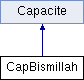
\includegraphics[height=2.000000cm]{class_cap_bismillah}
\end{center}
\end{figure}
\subsection*{Public Member Functions}
\begin{DoxyCompactItemize}
\item 
\mbox{\hyperlink{class_cap_bismillah_a0473031f39dc274f07c1f2b6e72ed6c7}{Cap\+Bismillah}} (\mbox{\hyperlink{class_ecran}{Ecran}} \&ecran, const std\+::weak\+\_\+ptr$<$ \mbox{\hyperlink{class_entite}{Entite}} $>$ \&lanceur)
\item 
void \mbox{\hyperlink{class_cap_bismillah_afc32f552a327af6f5759363d460f2eb7}{utiliser}} (\mbox{\hyperlink{def__type_8h_a87980cd8ee9533e561a73e8bbc728188}{proj\+\_\+container}} \&projectiles) override
\begin{DoxyCompactList}\small\item\em Active la capacite. \end{DoxyCompactList}\item 
void \mbox{\hyperlink{class_cap_bismillah_a3544607eb3d5e89bb6f5b6e2e2e89be0}{actualiser}} (\mbox{\hyperlink{def__type_8h_a87980cd8ee9533e561a73e8bbc728188}{proj\+\_\+container}} \&projectiles) override
\begin{DoxyCompactList}\small\item\em Active les effets de la capacit� \end{DoxyCompactList}\end{DoxyCompactItemize}
\subsection*{Additional Inherited Members}


\subsection{Constructor \& Destructor Documentation}
\mbox{\Hypertarget{class_cap_bismillah_a0473031f39dc274f07c1f2b6e72ed6c7}\label{class_cap_bismillah_a0473031f39dc274f07c1f2b6e72ed6c7}} 
\index{Cap\+Bismillah@{Cap\+Bismillah}!Cap\+Bismillah@{Cap\+Bismillah}}
\index{Cap\+Bismillah@{Cap\+Bismillah}!Cap\+Bismillah@{Cap\+Bismillah}}
\subsubsection{\texorpdfstring{Cap\+Bismillah()}{CapBismillah()}}
{\footnotesize\ttfamily Cap\+Bismillah\+::\+Cap\+Bismillah (\begin{DoxyParamCaption}\item[{\mbox{\hyperlink{class_ecran}{Ecran}} \&}]{ecran,  }\item[{const std\+::weak\+\_\+ptr$<$ \mbox{\hyperlink{class_entite}{Entite}} $>$ \&}]{lanceur }\end{DoxyParamCaption})\hspace{0.3cm}{\ttfamily [explicit]}}



\subsection{Member Function Documentation}
\mbox{\Hypertarget{class_cap_bismillah_a3544607eb3d5e89bb6f5b6e2e2e89be0}\label{class_cap_bismillah_a3544607eb3d5e89bb6f5b6e2e2e89be0}} 
\index{Cap\+Bismillah@{Cap\+Bismillah}!actualiser@{actualiser}}
\index{actualiser@{actualiser}!Cap\+Bismillah@{Cap\+Bismillah}}
\subsubsection{\texorpdfstring{actualiser()}{actualiser()}}
{\footnotesize\ttfamily Cap\+Bismillah\+::actualiser (\begin{DoxyParamCaption}\item[{\mbox{\hyperlink{def__type_8h_a87980cd8ee9533e561a73e8bbc728188}{proj\+\_\+container}} \&}]{projectiles }\end{DoxyParamCaption})\hspace{0.3cm}{\ttfamily [override]}, {\ttfamily [virtual]}}



Active les effets de la capacit� 

Cr�er 1 \mbox{\hyperlink{class_proj_piou}{Proj\+Piou}} � l\textquotesingle{}activation Actualise le timer 
\begin{DoxyParams}{Parameters}
{\em projectile} & Vecteur de tout les projectiles pr�sent � l\textquotesingle{}�cran \\
\hline
{\em vaisseau} & \mbox{\hyperlink{class_vaisseau}{Vaisseau}} qui a activ� la comp�tence \\
\hline
\end{DoxyParams}


Implements \mbox{\hyperlink{class_capacite_a85355aeb1d4acc049ed97da177acbd5f}{Capacite}}.

\mbox{\Hypertarget{class_cap_bismillah_afc32f552a327af6f5759363d460f2eb7}\label{class_cap_bismillah_afc32f552a327af6f5759363d460f2eb7}} 
\index{Cap\+Bismillah@{Cap\+Bismillah}!utiliser@{utiliser}}
\index{utiliser@{utiliser}!Cap\+Bismillah@{Cap\+Bismillah}}
\subsubsection{\texorpdfstring{utiliser()}{utiliser()}}
{\footnotesize\ttfamily Cap\+Bismillah\+::utiliser (\begin{DoxyParamCaption}\item[{\mbox{\hyperlink{def__type_8h_a87980cd8ee9533e561a73e8bbc728188}{proj\+\_\+container}} \&}]{projectiles }\end{DoxyParamCaption})\hspace{0.3cm}{\ttfamily [override]}, {\ttfamily [virtual]}}



Active la capacite. 


\begin{DoxyParams}{Parameters}
{\em x} & Abscisse de la position o� la capacite est utilis�e \\
\hline
{\em y} & Ordonn�e de la position o� la capacite est utilis�e\\
\hline
\end{DoxyParams}
Fonction Initialise la position de d�part et le timer 

Implements \mbox{\hyperlink{class_capacite_abac1434e2ac3ecc9e5afdafd9a7a4bed}{Capacite}}.



The documentation for this class was generated from the following files\+:\begin{DoxyCompactItemize}
\item 
src/\+Capacites/\mbox{\hyperlink{_cap_bismillah_beam_8h}{Cap\+Bismillah\+Beam.\+h}}\item 
src/\+Capacites/\mbox{\hyperlink{_cap_bismillah_beam_8cpp}{Cap\+Bismillah\+Beam.\+cpp}}\end{DoxyCompactItemize}

\hypertarget{class_cap_boing}{}\section{Cap\+Boing Class Reference}
\label{class_cap_boing}\index{Cap\+Boing@{Cap\+Boing}}


Classe Capacité de test.  




{\ttfamily \#include $<$Cap\+Boing.\+h$>$}

Inheritance diagram for Cap\+Boing\+:\begin{figure}[H]
\begin{center}
\leavevmode
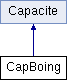
\includegraphics[height=2.000000cm]{class_cap_boing}
\end{center}
\end{figure}
\subsection*{Public Member Functions}
\begin{DoxyCompactItemize}
\item 
\mbox{\hyperlink{class_cap_boing_a9d315f24e4dfa2406956a9c53624d2ec}{Cap\+Boing}} (\mbox{\hyperlink{class_ecran}{Ecran}} \&ecran, const std\+::weak\+\_\+ptr$<$ \mbox{\hyperlink{class_entite}{Entite}} $>$ \&lanceur)
\begin{DoxyCompactList}\small\item\em Constructeur. \end{DoxyCompactList}\item 
\mbox{\hyperlink{class_cap_boing_a7f90c88c46fa87ff4c0fb66708648f96}{$\sim$\+Cap\+Boing}} () override=default
\begin{DoxyCompactList}\small\item\em Destructeur. \end{DoxyCompactList}\item 
void \mbox{\hyperlink{class_cap_boing_a879dfeba930a0be60873ef3403a35eb1}{utiliser}} (\mbox{\hyperlink{def__type_8h_a87980cd8ee9533e561a73e8bbc728188}{proj\+\_\+container}} \&projectiles) override
\begin{DoxyCompactList}\small\item\em Active la capacite. \end{DoxyCompactList}\item 
void \mbox{\hyperlink{class_cap_boing_a2bf6f58f93ff52263cf9926e4d91c239}{actualiser}} (\mbox{\hyperlink{def__type_8h_a87980cd8ee9533e561a73e8bbc728188}{proj\+\_\+container}} \&projectiles) override
\begin{DoxyCompactList}\small\item\em Active les effets de la capacité \end{DoxyCompactList}\end{DoxyCompactItemize}
\subsection*{Additional Inherited Members}


\subsection{Detailed Description}
Classe Capacité de test. 

Capacité qui créé 4 \mbox{\hyperlink{class_proj_boing}{Proj\+Boing}} à la position du lanceur Nom \+: Attaque Test Cooldown \+: 1000 ms 

\subsection{Constructor \& Destructor Documentation}
\mbox{\Hypertarget{class_cap_boing_a9d315f24e4dfa2406956a9c53624d2ec}\label{class_cap_boing_a9d315f24e4dfa2406956a9c53624d2ec}} 
\index{Cap\+Boing@{Cap\+Boing}!Cap\+Boing@{Cap\+Boing}}
\index{Cap\+Boing@{Cap\+Boing}!Cap\+Boing@{Cap\+Boing}}
\subsubsection{\texorpdfstring{Cap\+Boing()}{CapBoing()}}
{\footnotesize\ttfamily Cap\+Boing\+::\+Cap\+Boing (\begin{DoxyParamCaption}\item[{\mbox{\hyperlink{class_ecran}{Ecran}} \&}]{ecran,  }\item[{const std\+::weak\+\_\+ptr$<$ \mbox{\hyperlink{class_entite}{Entite}} $>$ \&}]{lanceur }\end{DoxyParamCaption})}



Constructeur. 

Initialisation de la capacité \mbox{\Hypertarget{class_cap_boing_a7f90c88c46fa87ff4c0fb66708648f96}\label{class_cap_boing_a7f90c88c46fa87ff4c0fb66708648f96}} 
\index{Cap\+Boing@{Cap\+Boing}!````~Cap\+Boing@{$\sim$\+Cap\+Boing}}
\index{````~Cap\+Boing@{$\sim$\+Cap\+Boing}!Cap\+Boing@{Cap\+Boing}}
\subsubsection{\texorpdfstring{$\sim$\+Cap\+Boing()}{~CapBoing()}}
{\footnotesize\ttfamily Cap\+Boing\+::$\sim$\+Cap\+Boing (\begin{DoxyParamCaption}{ }\end{DoxyParamCaption})\hspace{0.3cm}{\ttfamily [override]}, {\ttfamily [default]}}



Destructeur. 

Vide 

\subsection{Member Function Documentation}
\mbox{\Hypertarget{class_cap_boing_a2bf6f58f93ff52263cf9926e4d91c239}\label{class_cap_boing_a2bf6f58f93ff52263cf9926e4d91c239}} 
\index{Cap\+Boing@{Cap\+Boing}!actualiser@{actualiser}}
\index{actualiser@{actualiser}!Cap\+Boing@{Cap\+Boing}}
\subsubsection{\texorpdfstring{actualiser()}{actualiser()}}
{\footnotesize\ttfamily Cap\+Boing\+::actualiser (\begin{DoxyParamCaption}\item[{\mbox{\hyperlink{def__type_8h_a87980cd8ee9533e561a73e8bbc728188}{proj\+\_\+container}} \&}]{projectiles }\end{DoxyParamCaption})\hspace{0.3cm}{\ttfamily [override]}, {\ttfamily [virtual]}}



Active les effets de la capacité 


\begin{DoxyParams}{Parameters}
{\em projectile} & Vecteur de tout les projectiles présent à l\textquotesingle{}écran \\
\hline
{\em vaisseau} & \mbox{\hyperlink{class_vaisseau}{Vaisseau}} qui a activé la compétence\\
\hline
\end{DoxyParams}
Créer 4 \mbox{\hyperlink{class_proj_boing}{Proj\+Boing}} toutes les 5 frames Actualise le timer 

Implements \mbox{\hyperlink{class_capacite_a85355aeb1d4acc049ed97da177acbd5f}{Capacite}}.

\mbox{\Hypertarget{class_cap_boing_a879dfeba930a0be60873ef3403a35eb1}\label{class_cap_boing_a879dfeba930a0be60873ef3403a35eb1}} 
\index{Cap\+Boing@{Cap\+Boing}!utiliser@{utiliser}}
\index{utiliser@{utiliser}!Cap\+Boing@{Cap\+Boing}}
\subsubsection{\texorpdfstring{utiliser()}{utiliser()}}
{\footnotesize\ttfamily Cap\+Boing\+::utiliser (\begin{DoxyParamCaption}\item[{\mbox{\hyperlink{def__type_8h_a87980cd8ee9533e561a73e8bbc728188}{proj\+\_\+container}} \&}]{projectiles }\end{DoxyParamCaption})\hspace{0.3cm}{\ttfamily [override]}, {\ttfamily [virtual]}}



Active la capacite. 


\begin{DoxyParams}{Parameters}
{\em x} & Abscisse de la position où la capacite est utilisée \\
\hline
{\em y} & Ordonnée de la position où la capacite est utilisée\\
\hline
\end{DoxyParams}
Fonction Initialise la position de départ et le timer 

Implements \mbox{\hyperlink{class_capacite_abac1434e2ac3ecc9e5afdafd9a7a4bed}{Capacite}}.



The documentation for this class was generated from the following files\+:\begin{DoxyCompactItemize}
\item 
src/\+Capacites/\mbox{\hyperlink{_cap_boing_8h}{Cap\+Boing.\+h}}\item 
src/\+Capacites/\mbox{\hyperlink{_cap_boing_8cpp}{Cap\+Boing.\+cpp}}\end{DoxyCompactItemize}

\hypertarget{class_cap_bouclier_rond}{}\section{Référence de la classe Cap\+Bouclier\+Rond}
\label{class_cap_bouclier_rond}\index{Cap\+Bouclier\+Rond@{Cap\+Bouclier\+Rond}}


bouclier circulaire avec x PB  




{\ttfamily \#include $<$Cap\+Bouclier\+Rond.\+h$>$}



Graphe d\textquotesingle{}héritage de Cap\+Bouclier\+Rond\+:
% FIG 0


Graphe de collaboration de Cap\+Bouclier\+Rond\+:
% FIG 1
\subsection*{Fonctions membres publiques}
\begin{DoxyCompactItemize}
\item 
\hyperlink{class_cap_bouclier_rond_aec1b654b05d75943664c3d95ad2407ac}{Cap\+Bouclier\+Rond} (int niveau, \hyperlink{class_entite}{Entite} $\ast$Entite\+\_\+liee)
\begin{DoxyCompactList}\small\item\em \hyperlink{class_entite}{Entite} à laquelle s\textquotesingle{}applique le bouclier. \end{DoxyCompactList}\item 
void \hyperlink{class_cap_bouclier_rond_a058b65433ae77666bc6b64d787b455fb}{utiliser} (int x, int y) override
\begin{DoxyCompactList}\small\item\em Fonction virtuel qui active la capacite lorsqu\textquotesingle{}elle est appelée. \end{DoxyCompactList}\item 
void \hyperlink{class_cap_bouclier_rond_a4b272fe8aece56cb0e0ba7bf21b9d574}{actualiser} (std\+::vector$<$ \hyperlink{class_projectile}{Projectile} $\ast$$>$ \&G\+VP, \hyperlink{class_entite}{Entite} \&vaisseau, float temps\+Ecoule)
\begin{DoxyCompactList}\small\item\em Fonction virtuel qui active les effets de la capacité \end{DoxyCompactList}\end{DoxyCompactItemize}
\subsection*{Attributs protégés}
\begin{DoxyCompactItemize}
\item 
int \hyperlink{class_cap_bouclier_rond_a0dbbf591863880d6c2c46a8b87c5eba5}{pv\+M\+\_\+}
\item 
int \hyperlink{class_cap_bouclier_rond_a82d7dddc7f8857d19d3f3757718e06d7}{degats\+Coll\+\_\+}
\begin{DoxyCompactList}\small\item\em pv max du bouclier \end{DoxyCompactList}\item 
float \hyperlink{class_cap_bouclier_rond_abb59fc2be98b9d69c2fb1a3f832bdb19}{temps\+Max\+\_\+}
\begin{DoxyCompactList}\small\item\em dégats infligés lors d\textquotesingle{}une collisison avec une \hyperlink{class_entite}{Entite} collisionnable \end{DoxyCompactList}\item 
\hyperlink{class_entite}{Entite} $\ast$ \hyperlink{class_cap_bouclier_rond_a6667ab636d8eb5a8ba0b7b0bc0674b4b}{Entite\+\_\+liee\+\_\+}
\begin{DoxyCompactList}\small\item\em durée de vie du bouclier \end{DoxyCompactList}\end{DoxyCompactItemize}


\subsection{Description détaillée}
bouclier circulaire avec x PB 

Donne un bouclier circulaire qui entoure le vaisseau. Il est supprimé après un certain temps ( s sec) ou si ses (pb) PB tombent à zéro. Le bouclier est un projectile. Niveau 1 \+: Niveau supérieurs (idées) \+: augmente PB, temps de stase, réduit CD

Cooldown \+: 10sec 

\subsection{Documentation des constructeurs et destructeur}
\mbox{\Hypertarget{class_cap_bouclier_rond_aec1b654b05d75943664c3d95ad2407ac}\label{class_cap_bouclier_rond_aec1b654b05d75943664c3d95ad2407ac}} 
\index{Cap\+Bouclier\+Rond@{Cap\+Bouclier\+Rond}!Cap\+Bouclier\+Rond@{Cap\+Bouclier\+Rond}}
\index{Cap\+Bouclier\+Rond@{Cap\+Bouclier\+Rond}!Cap\+Bouclier\+Rond@{Cap\+Bouclier\+Rond}}
\subsubsection{\texorpdfstring{Cap\+Bouclier\+Rond()}{CapBouclierRond()}}
{\footnotesize\ttfamily Cap\+Bouclier\+Rond\+::\+Cap\+Bouclier\+Rond (\begin{DoxyParamCaption}\item[{int}]{niveau,  }\item[{\hyperlink{class_entite}{Entite} $\ast$}]{Entite\+\_\+liee }\end{DoxyParamCaption})}



\hyperlink{class_entite}{Entite} à laquelle s\textquotesingle{}applique le bouclier. 

Constructeur 
\begin{DoxyParams}{Paramètres}
{\em niveau} & niveau de la capacité \\
\hline
{\em Entite\+\_\+liee\+\_\+} & \hyperlink{class_entite}{Entite} à laquelle s\textquotesingle{}applique le bouclier\\
\hline
\end{DoxyParams}
Initialisation 

\subsection{Documentation des fonctions membres}
\mbox{\Hypertarget{class_cap_bouclier_rond_a4b272fe8aece56cb0e0ba7bf21b9d574}\label{class_cap_bouclier_rond_a4b272fe8aece56cb0e0ba7bf21b9d574}} 
\index{Cap\+Bouclier\+Rond@{Cap\+Bouclier\+Rond}!actualiser@{actualiser}}
\index{actualiser@{actualiser}!Cap\+Bouclier\+Rond@{Cap\+Bouclier\+Rond}}
\subsubsection{\texorpdfstring{actualiser()}{actualiser()}}
{\footnotesize\ttfamily void Cap\+Bouclier\+Rond\+::actualiser (\begin{DoxyParamCaption}\item[{std\+::vector$<$ \hyperlink{class_projectile}{Projectile} $\ast$$>$ \&}]{projectiles,  }\item[{\hyperlink{class_entite}{Entite} \&}]{vaisseau,  }\item[{float}]{temps\+Ecoule }\end{DoxyParamCaption})\hspace{0.3cm}{\ttfamily [virtual]}}



Fonction virtuel qui active les effets de la capacité 


\begin{DoxyParams}{Paramètres}
{\em projectile} & Vecteur de tout les projectiles présent à l\textquotesingle{}écran \\
\hline
{\em vaisseau} & \hyperlink{class_vaisseau}{Vaisseau} qui a activé la compétence \\
\hline
{\em temp\+Ecoule} & Temps écoulé depuis la dernière boucle\\
\hline
\end{DoxyParams}
Fonction virtuel qui gère la création de projectiles et des modifications à apporter au vaisseau 

Implémente \hyperlink{class_capacite_a75c9621d7a704fedb10ad29c6a697d64}{Capacite}.

\mbox{\Hypertarget{class_cap_bouclier_rond_a058b65433ae77666bc6b64d787b455fb}\label{class_cap_bouclier_rond_a058b65433ae77666bc6b64d787b455fb}} 
\index{Cap\+Bouclier\+Rond@{Cap\+Bouclier\+Rond}!utiliser@{utiliser}}
\index{utiliser@{utiliser}!Cap\+Bouclier\+Rond@{Cap\+Bouclier\+Rond}}
\subsubsection{\texorpdfstring{utiliser()}{utiliser()}}
{\footnotesize\ttfamily void Cap\+Bouclier\+Rond\+::utiliser (\begin{DoxyParamCaption}\item[{int}]{x,  }\item[{int}]{y }\end{DoxyParamCaption})\hspace{0.3cm}{\ttfamily [override]}, {\ttfamily [virtual]}}



Fonction virtuel qui active la capacite lorsqu\textquotesingle{}elle est appelée. 


\begin{DoxyParams}{Paramètres}
{\em x} & Abscisse de la position où la capacite est utilisée \\
\hline
{\em y} & Ordonnée de la position où la capacite est utilisée\\
\hline
\end{DoxyParams}
Fonction virtuel qui initialise la position de départ et le timer 

Implémente \hyperlink{class_capacite_a6f5e6efda11f80ab8538e23f5bdc6e79}{Capacite}.



\subsection{Documentation des données membres}
\mbox{\Hypertarget{class_cap_bouclier_rond_a82d7dddc7f8857d19d3f3757718e06d7}\label{class_cap_bouclier_rond_a82d7dddc7f8857d19d3f3757718e06d7}} 
\index{Cap\+Bouclier\+Rond@{Cap\+Bouclier\+Rond}!degats\+Coll\+\_\+@{degats\+Coll\+\_\+}}
\index{degats\+Coll\+\_\+@{degats\+Coll\+\_\+}!Cap\+Bouclier\+Rond@{Cap\+Bouclier\+Rond}}
\subsubsection{\texorpdfstring{degats\+Coll\+\_\+}{degatsColl\_}}
{\footnotesize\ttfamily int Cap\+Bouclier\+Rond\+::degats\+Coll\+\_\+\hspace{0.3cm}{\ttfamily [protected]}}



pv max du bouclier 

\mbox{\Hypertarget{class_cap_bouclier_rond_a6667ab636d8eb5a8ba0b7b0bc0674b4b}\label{class_cap_bouclier_rond_a6667ab636d8eb5a8ba0b7b0bc0674b4b}} 
\index{Cap\+Bouclier\+Rond@{Cap\+Bouclier\+Rond}!Entite\+\_\+liee\+\_\+@{Entite\+\_\+liee\+\_\+}}
\index{Entite\+\_\+liee\+\_\+@{Entite\+\_\+liee\+\_\+}!Cap\+Bouclier\+Rond@{Cap\+Bouclier\+Rond}}
\subsubsection{\texorpdfstring{Entite\+\_\+liee\+\_\+}{Entite\_liee\_}}
{\footnotesize\ttfamily \hyperlink{class_entite}{Entite}$\ast$ Cap\+Bouclier\+Rond\+::\+Entite\+\_\+liee\+\_\+\hspace{0.3cm}{\ttfamily [protected]}}



durée de vie du bouclier 

\mbox{\Hypertarget{class_cap_bouclier_rond_a0dbbf591863880d6c2c46a8b87c5eba5}\label{class_cap_bouclier_rond_a0dbbf591863880d6c2c46a8b87c5eba5}} 
\index{Cap\+Bouclier\+Rond@{Cap\+Bouclier\+Rond}!pv\+M\+\_\+@{pv\+M\+\_\+}}
\index{pv\+M\+\_\+@{pv\+M\+\_\+}!Cap\+Bouclier\+Rond@{Cap\+Bouclier\+Rond}}
\subsubsection{\texorpdfstring{pv\+M\+\_\+}{pvM\_}}
{\footnotesize\ttfamily int Cap\+Bouclier\+Rond\+::pv\+M\+\_\+\hspace{0.3cm}{\ttfamily [protected]}}

\mbox{\Hypertarget{class_cap_bouclier_rond_abb59fc2be98b9d69c2fb1a3f832bdb19}\label{class_cap_bouclier_rond_abb59fc2be98b9d69c2fb1a3f832bdb19}} 
\index{Cap\+Bouclier\+Rond@{Cap\+Bouclier\+Rond}!temps\+Max\+\_\+@{temps\+Max\+\_\+}}
\index{temps\+Max\+\_\+@{temps\+Max\+\_\+}!Cap\+Bouclier\+Rond@{Cap\+Bouclier\+Rond}}
\subsubsection{\texorpdfstring{temps\+Max\+\_\+}{tempsMax\_}}
{\footnotesize\ttfamily float Cap\+Bouclier\+Rond\+::temps\+Max\+\_\+\hspace{0.3cm}{\ttfamily [protected]}}



dégats infligés lors d\textquotesingle{}une collisison avec une \hyperlink{class_entite}{Entite} collisionnable 



La documentation de cette classe a été générée à partir des fichiers suivants \+:\begin{DoxyCompactItemize}
\item 
src/\+Capacites/\hyperlink{_cap_bouclier_rond_8h}{Cap\+Bouclier\+Rond.\+h}\item 
src/\+Capacites/\hyperlink{_cap_bouclier_rond_8cpp}{Cap\+Bouclier\+Rond.\+cpp}\end{DoxyCompactItemize}

\hypertarget{class_cap_dash}{}\section{Référence de la classe Cap\+Dash}
\label{class_cap_dash}\index{Cap\+Dash@{Cap\+Dash}}


Classe Capacité permettant de dash.  




{\ttfamily \#include $<$Cap\+Dash.\+h$>$}



Graphe d\textquotesingle{}héritage de Cap\+Dash\+:\nopagebreak
\begin{figure}[H]
\begin{center}
\leavevmode
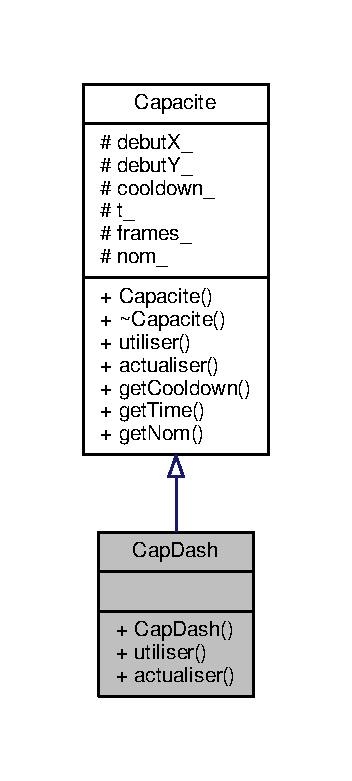
\includegraphics[width=138pt]{class_cap_dash__inherit__graph}
\end{center}
\end{figure}


Graphe de collaboration de Cap\+Dash\+:\nopagebreak
\begin{figure}[H]
\begin{center}
\leavevmode
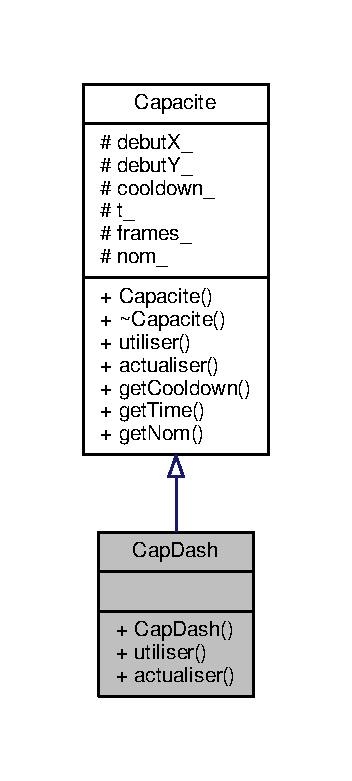
\includegraphics[width=138pt]{class_cap_dash__coll__graph}
\end{center}
\end{figure}
\subsection*{Fonctions membres publiques}
\begin{DoxyCompactItemize}
\item 
\hyperlink{class_cap_dash_ac38287e31284b6b5ac8add730830bfed}{Cap\+Dash} ()
\begin{DoxyCompactList}\small\item\em Constructeur. \end{DoxyCompactList}\item 
void \hyperlink{class_cap_dash_a8a0fe26c8b13d8a9f6cf5a95d6559f3d}{utiliser} (int x, int y) override
\begin{DoxyCompactList}\small\item\em Active la capacite. \end{DoxyCompactList}\item 
void \hyperlink{class_cap_dash_a23e3009b85288e7aadce2eb2b581fac0}{actualiser} (std\+::vector$<$ \hyperlink{class_projectile}{Projectile} $\ast$$>$ \&projectiles, \hyperlink{class_entite}{Entite} \&vaisseau, float temps\+Ecoule) override
\begin{DoxyCompactList}\small\item\em Active les effets de la capacité \end{DoxyCompactList}\end{DoxyCompactItemize}
\subsection*{Membres hérités additionnels}


\subsection{Description détaillée}
Classe Capacité permettant de dash. 

Modifie la vitesse du vaisseau peandant quelques frames Nom \+: Dash Cooldown \+: 500 ms 

\subsection{Documentation des constructeurs et destructeur}
\mbox{\Hypertarget{class_cap_dash_ac38287e31284b6b5ac8add730830bfed}\label{class_cap_dash_ac38287e31284b6b5ac8add730830bfed}} 
\index{Cap\+Dash@{Cap\+Dash}!Cap\+Dash@{Cap\+Dash}}
\index{Cap\+Dash@{Cap\+Dash}!Cap\+Dash@{Cap\+Dash}}
\subsubsection{\texorpdfstring{Cap\+Dash()}{CapDash()}}
{\footnotesize\ttfamily Cap\+Dash\+::\+Cap\+Dash (\begin{DoxyParamCaption}{ }\end{DoxyParamCaption})}



Constructeur. 

Initialisation de la capacité 

\subsection{Documentation des fonctions membres}
\mbox{\Hypertarget{class_cap_dash_a23e3009b85288e7aadce2eb2b581fac0}\label{class_cap_dash_a23e3009b85288e7aadce2eb2b581fac0}} 
\index{Cap\+Dash@{Cap\+Dash}!actualiser@{actualiser}}
\index{actualiser@{actualiser}!Cap\+Dash@{Cap\+Dash}}
\subsubsection{\texorpdfstring{actualiser()}{actualiser()}}
{\footnotesize\ttfamily Cap\+Dash\+::actualiser (\begin{DoxyParamCaption}\item[{std\+::vector$<$ \hyperlink{class_projectile}{Projectile} $\ast$$>$ \&}]{projectiles,  }\item[{\hyperlink{class_entite}{Entite} \&}]{vaisseau,  }\item[{float}]{temps\+Ecoule }\end{DoxyParamCaption})\hspace{0.3cm}{\ttfamily [override]}, {\ttfamily [virtual]}}



Active les effets de la capacité 


\begin{DoxyParams}[1]{Paramètres}
\mbox{\tt in,out}  & {\em projectile} & Vecteur de tout les projectiles présent à l\textquotesingle{}écran \\
\hline
\mbox{\tt in,out}  & {\em vaisseau} & \hyperlink{class_vaisseau}{Vaisseau} qui a activé la compétence \\
\hline
\mbox{\tt in}  & {\em temps\+Ecoule} & Temps écoulé en millisecondes\\
\hline
\end{DoxyParams}
Augmente la vitesse du vaisseau pour quelques frames Actualise le timer 

Implémente \hyperlink{class_capacite_a75c9621d7a704fedb10ad29c6a697d64}{Capacite}.

\mbox{\Hypertarget{class_cap_dash_a8a0fe26c8b13d8a9f6cf5a95d6559f3d}\label{class_cap_dash_a8a0fe26c8b13d8a9f6cf5a95d6559f3d}} 
\index{Cap\+Dash@{Cap\+Dash}!utiliser@{utiliser}}
\index{utiliser@{utiliser}!Cap\+Dash@{Cap\+Dash}}
\subsubsection{\texorpdfstring{utiliser()}{utiliser()}}
{\footnotesize\ttfamily Cap\+Dash\+::utiliser (\begin{DoxyParamCaption}\item[{int}]{x,  }\item[{int}]{y }\end{DoxyParamCaption})\hspace{0.3cm}{\ttfamily [override]}, {\ttfamily [virtual]}}



Active la capacite. 


\begin{DoxyParams}[1]{Paramètres}
\mbox{\tt in}  & {\em x} & Abscisse de la postion où la capacite est utilisée \\
\hline
\mbox{\tt in}  & {\em y} & Ordonnée de la postion où la capacite est utilisée\\
\hline
\end{DoxyParams}
Fonction Initialise la postion de départ et le timer 

Implémente \hyperlink{class_capacite_a6f5e6efda11f80ab8538e23f5bdc6e79}{Capacite}.



La documentation de cette classe a été générée à partir des fichiers suivants \+:\begin{DoxyCompactItemize}
\item 
src/\+Capacites/\hyperlink{_cap_dash_8h}{Cap\+Dash.\+h}\item 
src/\+Capacites/\hyperlink{_cap_dash_8cpp}{Cap\+Dash.\+cpp}\end{DoxyCompactItemize}

\hypertarget{class_cap_missile}{}\section{Référence de la classe Cap\+Missile}
\label{class_cap_missile}\index{Cap\+Missile@{Cap\+Missile}}


Classe Capacité de base.  




{\ttfamily \#include $<$Cap\+Missile.\+h$>$}



Graphe d\textquotesingle{}héritage de Cap\+Missile\+:
% FIG 0


Graphe de collaboration de Cap\+Missile\+:
% FIG 1
\subsection*{Fonctions membres publiques}
\begin{DoxyCompactItemize}
\item 
\hyperlink{class_cap_missile_a82f039eadaaba1712780a56598daae2a}{Cap\+Missile} ()
\item 
void \hyperlink{class_cap_missile_a4ba082615a3721083142549a4c8216ad}{utiliser} (int x, int y) override
\begin{DoxyCompactList}\small\item\em Active la capacite. \end{DoxyCompactList}\item 
void \hyperlink{class_cap_missile_adcb6a35330589c49910e6dd6cc7f2f7d}{actualiser} (std\+::vector$<$ \hyperlink{class_projectile}{Projectile} $\ast$$>$ \&projectiles, \hyperlink{class_entite}{Entite} \&vaisseau, float temps\+Ecoule) override
\begin{DoxyCompactList}\small\item\em Active les effets de la capacité \end{DoxyCompactList}\end{DoxyCompactItemize}
\subsection*{Membres hérités additionnels}


\subsection{Description détaillée}
Classe Capacité de base. 

Capacité qui créé 1 \hyperlink{class_proj_missile}{Proj\+Missile} à la position du lanceur Nom \+: Missile Cooldown \+: 5000 ms 

\subsection{Documentation des constructeurs et destructeur}
\mbox{\Hypertarget{class_cap_missile_a82f039eadaaba1712780a56598daae2a}\label{class_cap_missile_a82f039eadaaba1712780a56598daae2a}} 
\index{Cap\+Missile@{Cap\+Missile}!Cap\+Missile@{Cap\+Missile}}
\index{Cap\+Missile@{Cap\+Missile}!Cap\+Missile@{Cap\+Missile}}
\subsubsection{\texorpdfstring{Cap\+Missile()}{CapMissile()}}
{\footnotesize\ttfamily Cap\+Missile\+::\+Cap\+Missile (\begin{DoxyParamCaption}{ }\end{DoxyParamCaption})}



\subsection{Documentation des fonctions membres}
\mbox{\Hypertarget{class_cap_missile_adcb6a35330589c49910e6dd6cc7f2f7d}\label{class_cap_missile_adcb6a35330589c49910e6dd6cc7f2f7d}} 
\index{Cap\+Missile@{Cap\+Missile}!actualiser@{actualiser}}
\index{actualiser@{actualiser}!Cap\+Missile@{Cap\+Missile}}
\subsubsection{\texorpdfstring{actualiser()}{actualiser()}}
{\footnotesize\ttfamily Cap\+Missile\+::actualiser (\begin{DoxyParamCaption}\item[{std\+::vector$<$ \hyperlink{class_projectile}{Projectile} $\ast$$>$ \&}]{projectiles,  }\item[{\hyperlink{class_entite}{Entite} \&}]{vaisseau,  }\item[{float}]{temps\+Ecoule }\end{DoxyParamCaption})\hspace{0.3cm}{\ttfamily [override]}, {\ttfamily [virtual]}}



Active les effets de la capacité 

Créer 1 \hyperlink{class_proj_piou}{Proj\+Piou} à l\textquotesingle{}activation Actualise le timer 
\begin{DoxyParams}{Paramètres}
{\em projectile} & Vecteur de tout les projectiles présent à l\textquotesingle{}écran \\
\hline
{\em vaisseau} & \hyperlink{class_vaisseau}{Vaisseau} qui a activé la compétence \\
\hline
\end{DoxyParams}


Implémente \hyperlink{class_capacite_a75c9621d7a704fedb10ad29c6a697d64}{Capacite}.

\mbox{\Hypertarget{class_cap_missile_a4ba082615a3721083142549a4c8216ad}\label{class_cap_missile_a4ba082615a3721083142549a4c8216ad}} 
\index{Cap\+Missile@{Cap\+Missile}!utiliser@{utiliser}}
\index{utiliser@{utiliser}!Cap\+Missile@{Cap\+Missile}}
\subsubsection{\texorpdfstring{utiliser()}{utiliser()}}
{\footnotesize\ttfamily Cap\+Missile\+::utiliser (\begin{DoxyParamCaption}\item[{int}]{x,  }\item[{int}]{y }\end{DoxyParamCaption})\hspace{0.3cm}{\ttfamily [override]}, {\ttfamily [virtual]}}



Active la capacite. 


\begin{DoxyParams}{Paramètres}
{\em x} & Abscisse de la position où la capacite est utilisée \\
\hline
{\em y} & Ordonnée de la position où la capacite est utilisée\\
\hline
\end{DoxyParams}
Fonction Initialise la position de départ et le timer 

Implémente \hyperlink{class_capacite_a6f5e6efda11f80ab8538e23f5bdc6e79}{Capacite}.



La documentation de cette classe a été générée à partir des fichiers suivants \+:\begin{DoxyCompactItemize}
\item 
src/\+Capacites/\hyperlink{_cap_missile_8h}{Cap\+Missile.\+h}\item 
src/\+Capacites/\hyperlink{_cap_missile_8cpp}{Cap\+Missile.\+cpp}\end{DoxyCompactItemize}

\hypertarget{class_cap_piou}{}\section{Référence de la classe Cap\+Piou}
\label{class_cap_piou}\index{Cap\+Piou@{Cap\+Piou}}


{\ttfamily \#include $<$Cap\+Piou.\+h$>$}



Graphe d\textquotesingle{}héritage de Cap\+Piou\+:\nopagebreak
\begin{figure}[H]
\begin{center}
\leavevmode
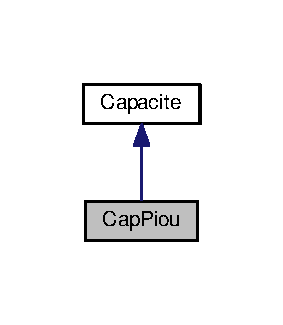
\includegraphics[width=136pt]{class_cap_piou__inherit__graph}
\end{center}
\end{figure}


Graphe de collaboration de Cap\+Piou\+:\nopagebreak
\begin{figure}[H]
\begin{center}
\leavevmode
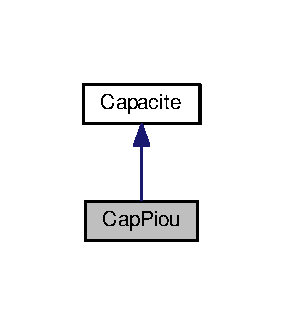
\includegraphics[width=136pt]{class_cap_piou__coll__graph}
\end{center}
\end{figure}
\subsection*{Fonctions membres publiques}
\begin{DoxyCompactItemize}
\item 
\hyperlink{class_cap_piou_aa2ed61fb1313a447cf8444399001750d}{Cap\+Piou} ()
\item 
\hyperlink{class_cap_piou_a35d7e0b0c14d6a6e01ba0a053a8a60bd}{$\sim$\+Cap\+Piou} ()
\item 
void \hyperlink{class_cap_piou_a20ed7a993ce209a3df246f655f107f22}{utiliser} (int x, int y)
\item 
void \hyperlink{class_cap_piou_aabdcaa253f10db2bca12e750005485fc}{actualiser} (std\+::vector$<$ \hyperlink{class_projectile}{Projectile} $\ast$$>$ \&projectiles, \hyperlink{class_entite}{Entite} $\ast$vaisseau)
\end{DoxyCompactItemize}
\subsection*{Membres hérités additionnels}


\subsection{Documentation des constructeurs et destructeur}
\mbox{\Hypertarget{class_cap_piou_aa2ed61fb1313a447cf8444399001750d}\label{class_cap_piou_aa2ed61fb1313a447cf8444399001750d}} 
\index{Cap\+Piou@{Cap\+Piou}!Cap\+Piou@{Cap\+Piou}}
\index{Cap\+Piou@{Cap\+Piou}!Cap\+Piou@{Cap\+Piou}}
\subsubsection{\texorpdfstring{Cap\+Piou()}{CapPiou()}}
{\footnotesize\ttfamily Cap\+Piou\+::\+Cap\+Piou (\begin{DoxyParamCaption}{ }\end{DoxyParamCaption})}

\mbox{\Hypertarget{class_cap_piou_a35d7e0b0c14d6a6e01ba0a053a8a60bd}\label{class_cap_piou_a35d7e0b0c14d6a6e01ba0a053a8a60bd}} 
\index{Cap\+Piou@{Cap\+Piou}!````~Cap\+Piou@{$\sim$\+Cap\+Piou}}
\index{````~Cap\+Piou@{$\sim$\+Cap\+Piou}!Cap\+Piou@{Cap\+Piou}}
\subsubsection{\texorpdfstring{$\sim$\+Cap\+Piou()}{~CapPiou()}}
{\footnotesize\ttfamily Cap\+Piou\+::$\sim$\+Cap\+Piou (\begin{DoxyParamCaption}{ }\end{DoxyParamCaption})}



\subsection{Documentation des fonctions membres}
\mbox{\Hypertarget{class_cap_piou_aabdcaa253f10db2bca12e750005485fc}\label{class_cap_piou_aabdcaa253f10db2bca12e750005485fc}} 
\index{Cap\+Piou@{Cap\+Piou}!actualiser@{actualiser}}
\index{actualiser@{actualiser}!Cap\+Piou@{Cap\+Piou}}
\subsubsection{\texorpdfstring{actualiser()}{actualiser()}}
{\footnotesize\ttfamily void Cap\+Piou\+::actualiser (\begin{DoxyParamCaption}\item[{std\+::vector$<$ \hyperlink{class_projectile}{Projectile} $\ast$$>$ \&}]{projectiles,  }\item[{\hyperlink{class_entite}{Entite} $\ast$}]{vaisseau }\end{DoxyParamCaption})\hspace{0.3cm}{\ttfamily [virtual]}}



Implémente \hyperlink{class_capacite_a7d4e86c20cd198960f25c0eb443148fe}{Capacite}.

\mbox{\Hypertarget{class_cap_piou_a20ed7a993ce209a3df246f655f107f22}\label{class_cap_piou_a20ed7a993ce209a3df246f655f107f22}} 
\index{Cap\+Piou@{Cap\+Piou}!utiliser@{utiliser}}
\index{utiliser@{utiliser}!Cap\+Piou@{Cap\+Piou}}
\subsubsection{\texorpdfstring{utiliser()}{utiliser()}}
{\footnotesize\ttfamily void Cap\+Piou\+::utiliser (\begin{DoxyParamCaption}\item[{int}]{x,  }\item[{int}]{y }\end{DoxyParamCaption})\hspace{0.3cm}{\ttfamily [virtual]}}



Implémente \hyperlink{class_capacite_a4d4f643987fcc2168567bf28a36ea418}{Capacite}.



La documentation de cette classe a été générée à partir des fichiers suivants \+:\begin{DoxyCompactItemize}
\item 
src/\hyperlink{_cap_piou_8h}{Cap\+Piou.\+h}\item 
src/\hyperlink{_cap_piou_8cpp}{Cap\+Piou.\+cpp}\end{DoxyCompactItemize}

\hypertarget{structstd_1_1experimental_1_1constexpr__optional__base}{}\section{std\+:\+:experimental\+:\+:constexpr\+\_\+optional\+\_\+base$<$ T $>$ Struct Template Reference}
\label{structstd_1_1experimental_1_1constexpr__optional__base}\index{std\+::experimental\+::constexpr\+\_\+optional\+\_\+base$<$ T $>$@{std\+::experimental\+::constexpr\+\_\+optional\+\_\+base$<$ T $>$}}


{\ttfamily \#include $<$optional.\+h$>$}

\subsection*{Public Member Functions}
\begin{DoxyCompactItemize}
\item 
constexpr \mbox{\hyperlink{structstd_1_1experimental_1_1constexpr__optional__base_a2de68e8d50f3b54344372c96c2123327}{constexpr\+\_\+optional\+\_\+base}} () noexcept
\item 
constexpr \mbox{\hyperlink{structstd_1_1experimental_1_1constexpr__optional__base_a215e82b0c75a04e871f55ab74def5653}{constexpr\+\_\+optional\+\_\+base}} (const T \&v)
\item 
constexpr \mbox{\hyperlink{structstd_1_1experimental_1_1constexpr__optional__base_a7a1c2735a3d7c86bdd4e179f9e291444}{constexpr\+\_\+optional\+\_\+base}} (T \&\&v)
\item 
{\footnotesize template$<$class... Args$>$ }\\constexpr \mbox{\hyperlink{structstd_1_1experimental_1_1constexpr__optional__base_a0ad7ea00451f21b435d46658be3eace6}{constexpr\+\_\+optional\+\_\+base}} (\mbox{\hyperlink{structstd_1_1experimental_1_1in__place__t}{in\+\_\+place\+\_\+t}}, Args \&\&... args)
\item 
{\footnotesize template$<$class U , class... Args, T\+R2\+\_\+\+O\+P\+T\+I\+O\+N\+A\+L\+\_\+\+R\+E\+Q\+U\+I\+R\+E\+S(is\+\_\+constructible$<$ T, std\+::initializer\+\_\+list$<$ U $>$$>$) $>$ }\\\mbox{\hyperlink{optional_8h_a7399114ed1c146a67741cdd1f681fcb5}{O\+P\+T\+I\+O\+N\+A\+L\+\_\+\+C\+O\+N\+S\+T\+E\+X\+P\+R\+\_\+\+I\+N\+I\+T\+\_\+\+L\+I\+ST}} \mbox{\hyperlink{structstd_1_1experimental_1_1constexpr__optional__base_aca7f761fe8d8a0e12295a590ff901654}{constexpr\+\_\+optional\+\_\+base}} (\mbox{\hyperlink{structstd_1_1experimental_1_1in__place__t}{in\+\_\+place\+\_\+t}}, std\+::initializer\+\_\+list$<$ U $>$ il, Args \&\&... args)
\item 
\mbox{\hyperlink{structstd_1_1experimental_1_1constexpr__optional__base_aa45afb4ed80eab963e850ca337956a95}{$\sim$constexpr\+\_\+optional\+\_\+base}} ()=default
\end{DoxyCompactItemize}
\subsection*{Public Attributes}
\begin{DoxyCompactItemize}
\item 
bool \mbox{\hyperlink{structstd_1_1experimental_1_1constexpr__optional__base_aef0ac13a059b733b785544ade26f3354}{init\+\_\+}}
\item 
\mbox{\hyperlink{unionstd_1_1experimental_1_1constexpr__storage__t}{constexpr\+\_\+storage\+\_\+t}}$<$ T $>$ \mbox{\hyperlink{structstd_1_1experimental_1_1constexpr__optional__base_a21e4f97ec2334b123f8e7c7a9d50c9b1}{storage\+\_\+}}
\end{DoxyCompactItemize}


\subsection{Constructor \& Destructor Documentation}
\mbox{\Hypertarget{structstd_1_1experimental_1_1constexpr__optional__base_a2de68e8d50f3b54344372c96c2123327}\label{structstd_1_1experimental_1_1constexpr__optional__base_a2de68e8d50f3b54344372c96c2123327}} 
\index{std\+::experimental\+::constexpr\+\_\+optional\+\_\+base@{std\+::experimental\+::constexpr\+\_\+optional\+\_\+base}!constexpr\+\_\+optional\+\_\+base@{constexpr\+\_\+optional\+\_\+base}}
\index{constexpr\+\_\+optional\+\_\+base@{constexpr\+\_\+optional\+\_\+base}!std\+::experimental\+::constexpr\+\_\+optional\+\_\+base@{std\+::experimental\+::constexpr\+\_\+optional\+\_\+base}}
\subsubsection{\texorpdfstring{constexpr\+\_\+optional\+\_\+base()}{constexpr\_optional\_base()}\hspace{0.1cm}{\footnotesize\ttfamily [1/5]}}
{\footnotesize\ttfamily template$<$class T $>$ \\
constexpr \mbox{\hyperlink{structstd_1_1experimental_1_1constexpr__optional__base}{std\+::experimental\+::constexpr\+\_\+optional\+\_\+base}}$<$ T $>$\+::\mbox{\hyperlink{structstd_1_1experimental_1_1constexpr__optional__base}{constexpr\+\_\+optional\+\_\+base}} (\begin{DoxyParamCaption}{ }\end{DoxyParamCaption})\hspace{0.3cm}{\ttfamily [inline]}, {\ttfamily [noexcept]}}

\mbox{\Hypertarget{structstd_1_1experimental_1_1constexpr__optional__base_a215e82b0c75a04e871f55ab74def5653}\label{structstd_1_1experimental_1_1constexpr__optional__base_a215e82b0c75a04e871f55ab74def5653}} 
\index{std\+::experimental\+::constexpr\+\_\+optional\+\_\+base@{std\+::experimental\+::constexpr\+\_\+optional\+\_\+base}!constexpr\+\_\+optional\+\_\+base@{constexpr\+\_\+optional\+\_\+base}}
\index{constexpr\+\_\+optional\+\_\+base@{constexpr\+\_\+optional\+\_\+base}!std\+::experimental\+::constexpr\+\_\+optional\+\_\+base@{std\+::experimental\+::constexpr\+\_\+optional\+\_\+base}}
\subsubsection{\texorpdfstring{constexpr\+\_\+optional\+\_\+base()}{constexpr\_optional\_base()}\hspace{0.1cm}{\footnotesize\ttfamily [2/5]}}
{\footnotesize\ttfamily template$<$class T $>$ \\
constexpr \mbox{\hyperlink{structstd_1_1experimental_1_1constexpr__optional__base}{std\+::experimental\+::constexpr\+\_\+optional\+\_\+base}}$<$ T $>$\+::\mbox{\hyperlink{structstd_1_1experimental_1_1constexpr__optional__base}{constexpr\+\_\+optional\+\_\+base}} (\begin{DoxyParamCaption}\item[{const T \&}]{v }\end{DoxyParamCaption})\hspace{0.3cm}{\ttfamily [inline]}, {\ttfamily [explicit]}}

\mbox{\Hypertarget{structstd_1_1experimental_1_1constexpr__optional__base_a7a1c2735a3d7c86bdd4e179f9e291444}\label{structstd_1_1experimental_1_1constexpr__optional__base_a7a1c2735a3d7c86bdd4e179f9e291444}} 
\index{std\+::experimental\+::constexpr\+\_\+optional\+\_\+base@{std\+::experimental\+::constexpr\+\_\+optional\+\_\+base}!constexpr\+\_\+optional\+\_\+base@{constexpr\+\_\+optional\+\_\+base}}
\index{constexpr\+\_\+optional\+\_\+base@{constexpr\+\_\+optional\+\_\+base}!std\+::experimental\+::constexpr\+\_\+optional\+\_\+base@{std\+::experimental\+::constexpr\+\_\+optional\+\_\+base}}
\subsubsection{\texorpdfstring{constexpr\+\_\+optional\+\_\+base()}{constexpr\_optional\_base()}\hspace{0.1cm}{\footnotesize\ttfamily [3/5]}}
{\footnotesize\ttfamily template$<$class T $>$ \\
constexpr \mbox{\hyperlink{structstd_1_1experimental_1_1constexpr__optional__base}{std\+::experimental\+::constexpr\+\_\+optional\+\_\+base}}$<$ T $>$\+::\mbox{\hyperlink{structstd_1_1experimental_1_1constexpr__optional__base}{constexpr\+\_\+optional\+\_\+base}} (\begin{DoxyParamCaption}\item[{T \&\&}]{v }\end{DoxyParamCaption})\hspace{0.3cm}{\ttfamily [inline]}, {\ttfamily [explicit]}}

\mbox{\Hypertarget{structstd_1_1experimental_1_1constexpr__optional__base_a0ad7ea00451f21b435d46658be3eace6}\label{structstd_1_1experimental_1_1constexpr__optional__base_a0ad7ea00451f21b435d46658be3eace6}} 
\index{std\+::experimental\+::constexpr\+\_\+optional\+\_\+base@{std\+::experimental\+::constexpr\+\_\+optional\+\_\+base}!constexpr\+\_\+optional\+\_\+base@{constexpr\+\_\+optional\+\_\+base}}
\index{constexpr\+\_\+optional\+\_\+base@{constexpr\+\_\+optional\+\_\+base}!std\+::experimental\+::constexpr\+\_\+optional\+\_\+base@{std\+::experimental\+::constexpr\+\_\+optional\+\_\+base}}
\subsubsection{\texorpdfstring{constexpr\+\_\+optional\+\_\+base()}{constexpr\_optional\_base()}\hspace{0.1cm}{\footnotesize\ttfamily [4/5]}}
{\footnotesize\ttfamily template$<$class T $>$ \\
template$<$class... Args$>$ \\
constexpr \mbox{\hyperlink{structstd_1_1experimental_1_1constexpr__optional__base}{std\+::experimental\+::constexpr\+\_\+optional\+\_\+base}}$<$ T $>$\+::\mbox{\hyperlink{structstd_1_1experimental_1_1constexpr__optional__base}{constexpr\+\_\+optional\+\_\+base}} (\begin{DoxyParamCaption}\item[{\mbox{\hyperlink{structstd_1_1experimental_1_1in__place__t}{in\+\_\+place\+\_\+t}}}]{,  }\item[{Args \&\&...}]{args }\end{DoxyParamCaption})\hspace{0.3cm}{\ttfamily [inline]}, {\ttfamily [explicit]}}

\mbox{\Hypertarget{structstd_1_1experimental_1_1constexpr__optional__base_aca7f761fe8d8a0e12295a590ff901654}\label{structstd_1_1experimental_1_1constexpr__optional__base_aca7f761fe8d8a0e12295a590ff901654}} 
\index{std\+::experimental\+::constexpr\+\_\+optional\+\_\+base@{std\+::experimental\+::constexpr\+\_\+optional\+\_\+base}!constexpr\+\_\+optional\+\_\+base@{constexpr\+\_\+optional\+\_\+base}}
\index{constexpr\+\_\+optional\+\_\+base@{constexpr\+\_\+optional\+\_\+base}!std\+::experimental\+::constexpr\+\_\+optional\+\_\+base@{std\+::experimental\+::constexpr\+\_\+optional\+\_\+base}}
\subsubsection{\texorpdfstring{constexpr\+\_\+optional\+\_\+base()}{constexpr\_optional\_base()}\hspace{0.1cm}{\footnotesize\ttfamily [5/5]}}
{\footnotesize\ttfamily template$<$class T $>$ \\
template$<$class U , class... Args, T\+R2\+\_\+\+O\+P\+T\+I\+O\+N\+A\+L\+\_\+\+R\+E\+Q\+U\+I\+R\+E\+S(is\+\_\+constructible$<$ T, std\+::initializer\+\_\+list$<$ U $>$$>$) $>$ \\
\mbox{\hyperlink{optional_8h_a7399114ed1c146a67741cdd1f681fcb5}{O\+P\+T\+I\+O\+N\+A\+L\+\_\+\+C\+O\+N\+S\+T\+E\+X\+P\+R\+\_\+\+I\+N\+I\+T\+\_\+\+L\+I\+ST}} \mbox{\hyperlink{structstd_1_1experimental_1_1constexpr__optional__base}{std\+::experimental\+::constexpr\+\_\+optional\+\_\+base}}$<$ T $>$\+::\mbox{\hyperlink{structstd_1_1experimental_1_1constexpr__optional__base}{constexpr\+\_\+optional\+\_\+base}} (\begin{DoxyParamCaption}\item[{\mbox{\hyperlink{structstd_1_1experimental_1_1in__place__t}{in\+\_\+place\+\_\+t}}}]{,  }\item[{std\+::initializer\+\_\+list$<$ U $>$}]{il,  }\item[{Args \&\&...}]{args }\end{DoxyParamCaption})\hspace{0.3cm}{\ttfamily [inline]}, {\ttfamily [explicit]}}

\mbox{\Hypertarget{structstd_1_1experimental_1_1constexpr__optional__base_aa45afb4ed80eab963e850ca337956a95}\label{structstd_1_1experimental_1_1constexpr__optional__base_aa45afb4ed80eab963e850ca337956a95}} 
\index{std\+::experimental\+::constexpr\+\_\+optional\+\_\+base@{std\+::experimental\+::constexpr\+\_\+optional\+\_\+base}!````~constexpr\+\_\+optional\+\_\+base@{$\sim$constexpr\+\_\+optional\+\_\+base}}
\index{````~constexpr\+\_\+optional\+\_\+base@{$\sim$constexpr\+\_\+optional\+\_\+base}!std\+::experimental\+::constexpr\+\_\+optional\+\_\+base@{std\+::experimental\+::constexpr\+\_\+optional\+\_\+base}}
\subsubsection{\texorpdfstring{$\sim$constexpr\+\_\+optional\+\_\+base()}{~constexpr\_optional\_base()}}
{\footnotesize\ttfamily template$<$class T $>$ \\
\mbox{\hyperlink{structstd_1_1experimental_1_1constexpr__optional__base}{std\+::experimental\+::constexpr\+\_\+optional\+\_\+base}}$<$ T $>$\+::$\sim$\mbox{\hyperlink{structstd_1_1experimental_1_1constexpr__optional__base}{constexpr\+\_\+optional\+\_\+base}} (\begin{DoxyParamCaption}{ }\end{DoxyParamCaption})\hspace{0.3cm}{\ttfamily [default]}}



\subsection{Member Data Documentation}
\mbox{\Hypertarget{structstd_1_1experimental_1_1constexpr__optional__base_aef0ac13a059b733b785544ade26f3354}\label{structstd_1_1experimental_1_1constexpr__optional__base_aef0ac13a059b733b785544ade26f3354}} 
\index{std\+::experimental\+::constexpr\+\_\+optional\+\_\+base@{std\+::experimental\+::constexpr\+\_\+optional\+\_\+base}!init\+\_\+@{init\+\_\+}}
\index{init\+\_\+@{init\+\_\+}!std\+::experimental\+::constexpr\+\_\+optional\+\_\+base@{std\+::experimental\+::constexpr\+\_\+optional\+\_\+base}}
\subsubsection{\texorpdfstring{init\+\_\+}{init\_}}
{\footnotesize\ttfamily template$<$class T $>$ \\
bool \mbox{\hyperlink{structstd_1_1experimental_1_1constexpr__optional__base}{std\+::experimental\+::constexpr\+\_\+optional\+\_\+base}}$<$ T $>$\+::init\+\_\+}

\mbox{\Hypertarget{structstd_1_1experimental_1_1constexpr__optional__base_a21e4f97ec2334b123f8e7c7a9d50c9b1}\label{structstd_1_1experimental_1_1constexpr__optional__base_a21e4f97ec2334b123f8e7c7a9d50c9b1}} 
\index{std\+::experimental\+::constexpr\+\_\+optional\+\_\+base@{std\+::experimental\+::constexpr\+\_\+optional\+\_\+base}!storage\+\_\+@{storage\+\_\+}}
\index{storage\+\_\+@{storage\+\_\+}!std\+::experimental\+::constexpr\+\_\+optional\+\_\+base@{std\+::experimental\+::constexpr\+\_\+optional\+\_\+base}}
\subsubsection{\texorpdfstring{storage\+\_\+}{storage\_}}
{\footnotesize\ttfamily template$<$class T $>$ \\
\mbox{\hyperlink{unionstd_1_1experimental_1_1constexpr__storage__t}{constexpr\+\_\+storage\+\_\+t}}$<$T$>$ \mbox{\hyperlink{structstd_1_1experimental_1_1constexpr__optional__base}{std\+::experimental\+::constexpr\+\_\+optional\+\_\+base}}$<$ T $>$\+::storage\+\_\+}



The documentation for this struct was generated from the following file\+:\begin{DoxyCompactItemize}
\item 
src/\+Utilitaires/\mbox{\hyperlink{optional_8h}{optional.\+h}}\end{DoxyCompactItemize}

\hypertarget{unionstd_1_1experimental_1_1constexpr__storage__t}{}\section{std\+:\+:experimental\+:\+:constexpr\+\_\+storage\+\_\+t$<$ T $>$ Union Template Reference}
\label{unionstd_1_1experimental_1_1constexpr__storage__t}\index{std\+::experimental\+::constexpr\+\_\+storage\+\_\+t$<$ T $>$@{std\+::experimental\+::constexpr\+\_\+storage\+\_\+t$<$ T $>$}}


{\ttfamily \#include $<$optional.\+h$>$}

\subsection*{Public Member Functions}
\begin{DoxyCompactItemize}
\item 
constexpr \mbox{\hyperlink{unionstd_1_1experimental_1_1constexpr__storage__t_a453f1fc4d9790ed1a15175a9c13fe517}{constexpr\+\_\+storage\+\_\+t}} (\mbox{\hyperlink{structstd_1_1experimental_1_1trivial__init__t}{trivial\+\_\+init\+\_\+t}}) noexcept
\item 
{\footnotesize template$<$class... Args$>$ }\\constexpr \mbox{\hyperlink{unionstd_1_1experimental_1_1constexpr__storage__t_a643de5b95dac28e87811c7ff4890cd19}{constexpr\+\_\+storage\+\_\+t}} (Args \&\&... args)
\item 
\mbox{\hyperlink{unionstd_1_1experimental_1_1constexpr__storage__t_a91464aa4649be3df9952707782a58a6d}{$\sim$constexpr\+\_\+storage\+\_\+t}} ()=default
\end{DoxyCompactItemize}
\subsection*{Public Attributes}
\begin{DoxyCompactItemize}
\item 
unsigned char \mbox{\hyperlink{unionstd_1_1experimental_1_1constexpr__storage__t_abab3e99e25b519d05a2b32c3748cf759}{dummy\+\_\+}}
\item 
T \mbox{\hyperlink{unionstd_1_1experimental_1_1constexpr__storage__t_ab0f056b5b1e7bfde0dc04629fd0b9ade}{value\+\_\+}}
\end{DoxyCompactItemize}


\subsection{Constructor \& Destructor Documentation}
\mbox{\Hypertarget{unionstd_1_1experimental_1_1constexpr__storage__t_a453f1fc4d9790ed1a15175a9c13fe517}\label{unionstd_1_1experimental_1_1constexpr__storage__t_a453f1fc4d9790ed1a15175a9c13fe517}} 
\index{std\+::experimental\+::constexpr\+\_\+storage\+\_\+t@{std\+::experimental\+::constexpr\+\_\+storage\+\_\+t}!constexpr\+\_\+storage\+\_\+t@{constexpr\+\_\+storage\+\_\+t}}
\index{constexpr\+\_\+storage\+\_\+t@{constexpr\+\_\+storage\+\_\+t}!std\+::experimental\+::constexpr\+\_\+storage\+\_\+t@{std\+::experimental\+::constexpr\+\_\+storage\+\_\+t}}
\subsubsection{\texorpdfstring{constexpr\+\_\+storage\+\_\+t()}{constexpr\_storage\_t()}\hspace{0.1cm}{\footnotesize\ttfamily [1/2]}}
{\footnotesize\ttfamily template$<$class T$>$ \\
constexpr \mbox{\hyperlink{unionstd_1_1experimental_1_1constexpr__storage__t}{std\+::experimental\+::constexpr\+\_\+storage\+\_\+t}}$<$ T $>$\+::\mbox{\hyperlink{unionstd_1_1experimental_1_1constexpr__storage__t}{constexpr\+\_\+storage\+\_\+t}} (\begin{DoxyParamCaption}\item[{\mbox{\hyperlink{structstd_1_1experimental_1_1trivial__init__t}{trivial\+\_\+init\+\_\+t}}}]{ }\end{DoxyParamCaption})\hspace{0.3cm}{\ttfamily [inline]}, {\ttfamily [noexcept]}}

\mbox{\Hypertarget{unionstd_1_1experimental_1_1constexpr__storage__t_a643de5b95dac28e87811c7ff4890cd19}\label{unionstd_1_1experimental_1_1constexpr__storage__t_a643de5b95dac28e87811c7ff4890cd19}} 
\index{std\+::experimental\+::constexpr\+\_\+storage\+\_\+t@{std\+::experimental\+::constexpr\+\_\+storage\+\_\+t}!constexpr\+\_\+storage\+\_\+t@{constexpr\+\_\+storage\+\_\+t}}
\index{constexpr\+\_\+storage\+\_\+t@{constexpr\+\_\+storage\+\_\+t}!std\+::experimental\+::constexpr\+\_\+storage\+\_\+t@{std\+::experimental\+::constexpr\+\_\+storage\+\_\+t}}
\subsubsection{\texorpdfstring{constexpr\+\_\+storage\+\_\+t()}{constexpr\_storage\_t()}\hspace{0.1cm}{\footnotesize\ttfamily [2/2]}}
{\footnotesize\ttfamily template$<$class T$>$ \\
template$<$class... Args$>$ \\
constexpr \mbox{\hyperlink{unionstd_1_1experimental_1_1constexpr__storage__t}{std\+::experimental\+::constexpr\+\_\+storage\+\_\+t}}$<$ T $>$\+::\mbox{\hyperlink{unionstd_1_1experimental_1_1constexpr__storage__t}{constexpr\+\_\+storage\+\_\+t}} (\begin{DoxyParamCaption}\item[{Args \&\&...}]{args }\end{DoxyParamCaption})\hspace{0.3cm}{\ttfamily [inline]}}

\mbox{\Hypertarget{unionstd_1_1experimental_1_1constexpr__storage__t_a91464aa4649be3df9952707782a58a6d}\label{unionstd_1_1experimental_1_1constexpr__storage__t_a91464aa4649be3df9952707782a58a6d}} 
\index{std\+::experimental\+::constexpr\+\_\+storage\+\_\+t@{std\+::experimental\+::constexpr\+\_\+storage\+\_\+t}!````~constexpr\+\_\+storage\+\_\+t@{$\sim$constexpr\+\_\+storage\+\_\+t}}
\index{````~constexpr\+\_\+storage\+\_\+t@{$\sim$constexpr\+\_\+storage\+\_\+t}!std\+::experimental\+::constexpr\+\_\+storage\+\_\+t@{std\+::experimental\+::constexpr\+\_\+storage\+\_\+t}}
\subsubsection{\texorpdfstring{$\sim$constexpr\+\_\+storage\+\_\+t()}{~constexpr\_storage\_t()}}
{\footnotesize\ttfamily template$<$class T$>$ \\
\mbox{\hyperlink{unionstd_1_1experimental_1_1constexpr__storage__t}{std\+::experimental\+::constexpr\+\_\+storage\+\_\+t}}$<$ T $>$\+::$\sim$\mbox{\hyperlink{unionstd_1_1experimental_1_1constexpr__storage__t}{constexpr\+\_\+storage\+\_\+t}} (\begin{DoxyParamCaption}{ }\end{DoxyParamCaption})\hspace{0.3cm}{\ttfamily [default]}}



\subsection{Member Data Documentation}
\mbox{\Hypertarget{unionstd_1_1experimental_1_1constexpr__storage__t_abab3e99e25b519d05a2b32c3748cf759}\label{unionstd_1_1experimental_1_1constexpr__storage__t_abab3e99e25b519d05a2b32c3748cf759}} 
\index{std\+::experimental\+::constexpr\+\_\+storage\+\_\+t@{std\+::experimental\+::constexpr\+\_\+storage\+\_\+t}!dummy\+\_\+@{dummy\+\_\+}}
\index{dummy\+\_\+@{dummy\+\_\+}!std\+::experimental\+::constexpr\+\_\+storage\+\_\+t@{std\+::experimental\+::constexpr\+\_\+storage\+\_\+t}}
\subsubsection{\texorpdfstring{dummy\+\_\+}{dummy\_}}
{\footnotesize\ttfamily template$<$class T$>$ \\
unsigned char \mbox{\hyperlink{unionstd_1_1experimental_1_1constexpr__storage__t}{std\+::experimental\+::constexpr\+\_\+storage\+\_\+t}}$<$ T $>$\+::dummy\+\_\+}

\mbox{\Hypertarget{unionstd_1_1experimental_1_1constexpr__storage__t_ab0f056b5b1e7bfde0dc04629fd0b9ade}\label{unionstd_1_1experimental_1_1constexpr__storage__t_ab0f056b5b1e7bfde0dc04629fd0b9ade}} 
\index{std\+::experimental\+::constexpr\+\_\+storage\+\_\+t@{std\+::experimental\+::constexpr\+\_\+storage\+\_\+t}!value\+\_\+@{value\+\_\+}}
\index{value\+\_\+@{value\+\_\+}!std\+::experimental\+::constexpr\+\_\+storage\+\_\+t@{std\+::experimental\+::constexpr\+\_\+storage\+\_\+t}}
\subsubsection{\texorpdfstring{value\+\_\+}{value\_}}
{\footnotesize\ttfamily template$<$class T$>$ \\
T \mbox{\hyperlink{unionstd_1_1experimental_1_1constexpr__storage__t}{std\+::experimental\+::constexpr\+\_\+storage\+\_\+t}}$<$ T $>$\+::value\+\_\+}



The documentation for this union was generated from the following file\+:\begin{DoxyCompactItemize}
\item 
src/\+Utilitaires/\mbox{\hyperlink{optional_8h}{optional.\+h}}\end{DoxyCompactItemize}

\hypertarget{struct_element_vague}{}\section{Référence de la structure Element\+Vague}
\label{struct_element_vague}\index{Element\+Vague@{Element\+Vague}}


{\ttfamily \#include $<$Vague.\+h$>$}



Graphe de collaboration de Element\+Vague\+:
% FIG 0
\subsection*{Attributs publics}
\begin{DoxyCompactItemize}
\item 
float \hyperlink{struct_element_vague_af6645ffc5fbc3be59dbf5063a78f8e36}{t}
\item 
\hyperlink{class_vaisseau}{Vaisseau} $\ast$ \hyperlink{struct_element_vague_a74ef9460cb2ccf37f07caa28b48959ec}{v}
\item 
bool \hyperlink{struct_element_vague_ab0bd206a38ece486f6f5bb9ec76ff36b}{active}
\end{DoxyCompactItemize}


\subsection{Documentation des données membres}
\mbox{\Hypertarget{struct_element_vague_ab0bd206a38ece486f6f5bb9ec76ff36b}\label{struct_element_vague_ab0bd206a38ece486f6f5bb9ec76ff36b}} 
\index{Element\+Vague@{Element\+Vague}!active@{active}}
\index{active@{active}!Element\+Vague@{Element\+Vague}}
\subsubsection{\texorpdfstring{active}{active}}
{\footnotesize\ttfamily bool Element\+Vague\+::active}

\mbox{\Hypertarget{struct_element_vague_af6645ffc5fbc3be59dbf5063a78f8e36}\label{struct_element_vague_af6645ffc5fbc3be59dbf5063a78f8e36}} 
\index{Element\+Vague@{Element\+Vague}!t@{t}}
\index{t@{t}!Element\+Vague@{Element\+Vague}}
\subsubsection{\texorpdfstring{t}{t}}
{\footnotesize\ttfamily float Element\+Vague\+::t}

\mbox{\Hypertarget{struct_element_vague_a74ef9460cb2ccf37f07caa28b48959ec}\label{struct_element_vague_a74ef9460cb2ccf37f07caa28b48959ec}} 
\index{Element\+Vague@{Element\+Vague}!v@{v}}
\index{v@{v}!Element\+Vague@{Element\+Vague}}
\subsubsection{\texorpdfstring{v}{v}}
{\footnotesize\ttfamily \hyperlink{class_vaisseau}{Vaisseau}$\ast$ Element\+Vague\+::v}



La documentation de cette structure a été générée à partir du fichier suivant \+:\begin{DoxyCompactItemize}
\item 
src/\+Pattern/\hyperlink{_vague_8h}{Vague.\+h}\end{DoxyCompactItemize}

\hypertarget{class_entite}{}\section{Référence de la classe Entite}
\label{class_entite}\index{Entite@{Entite}}


Classe virtuelle qui définit une entité  




{\ttfamily \#include $<$Entite.\+h$>$}



Graphe d\textquotesingle{}héritage de Entite\+:\nopagebreak
\begin{figure}[H]
\begin{center}
\leavevmode
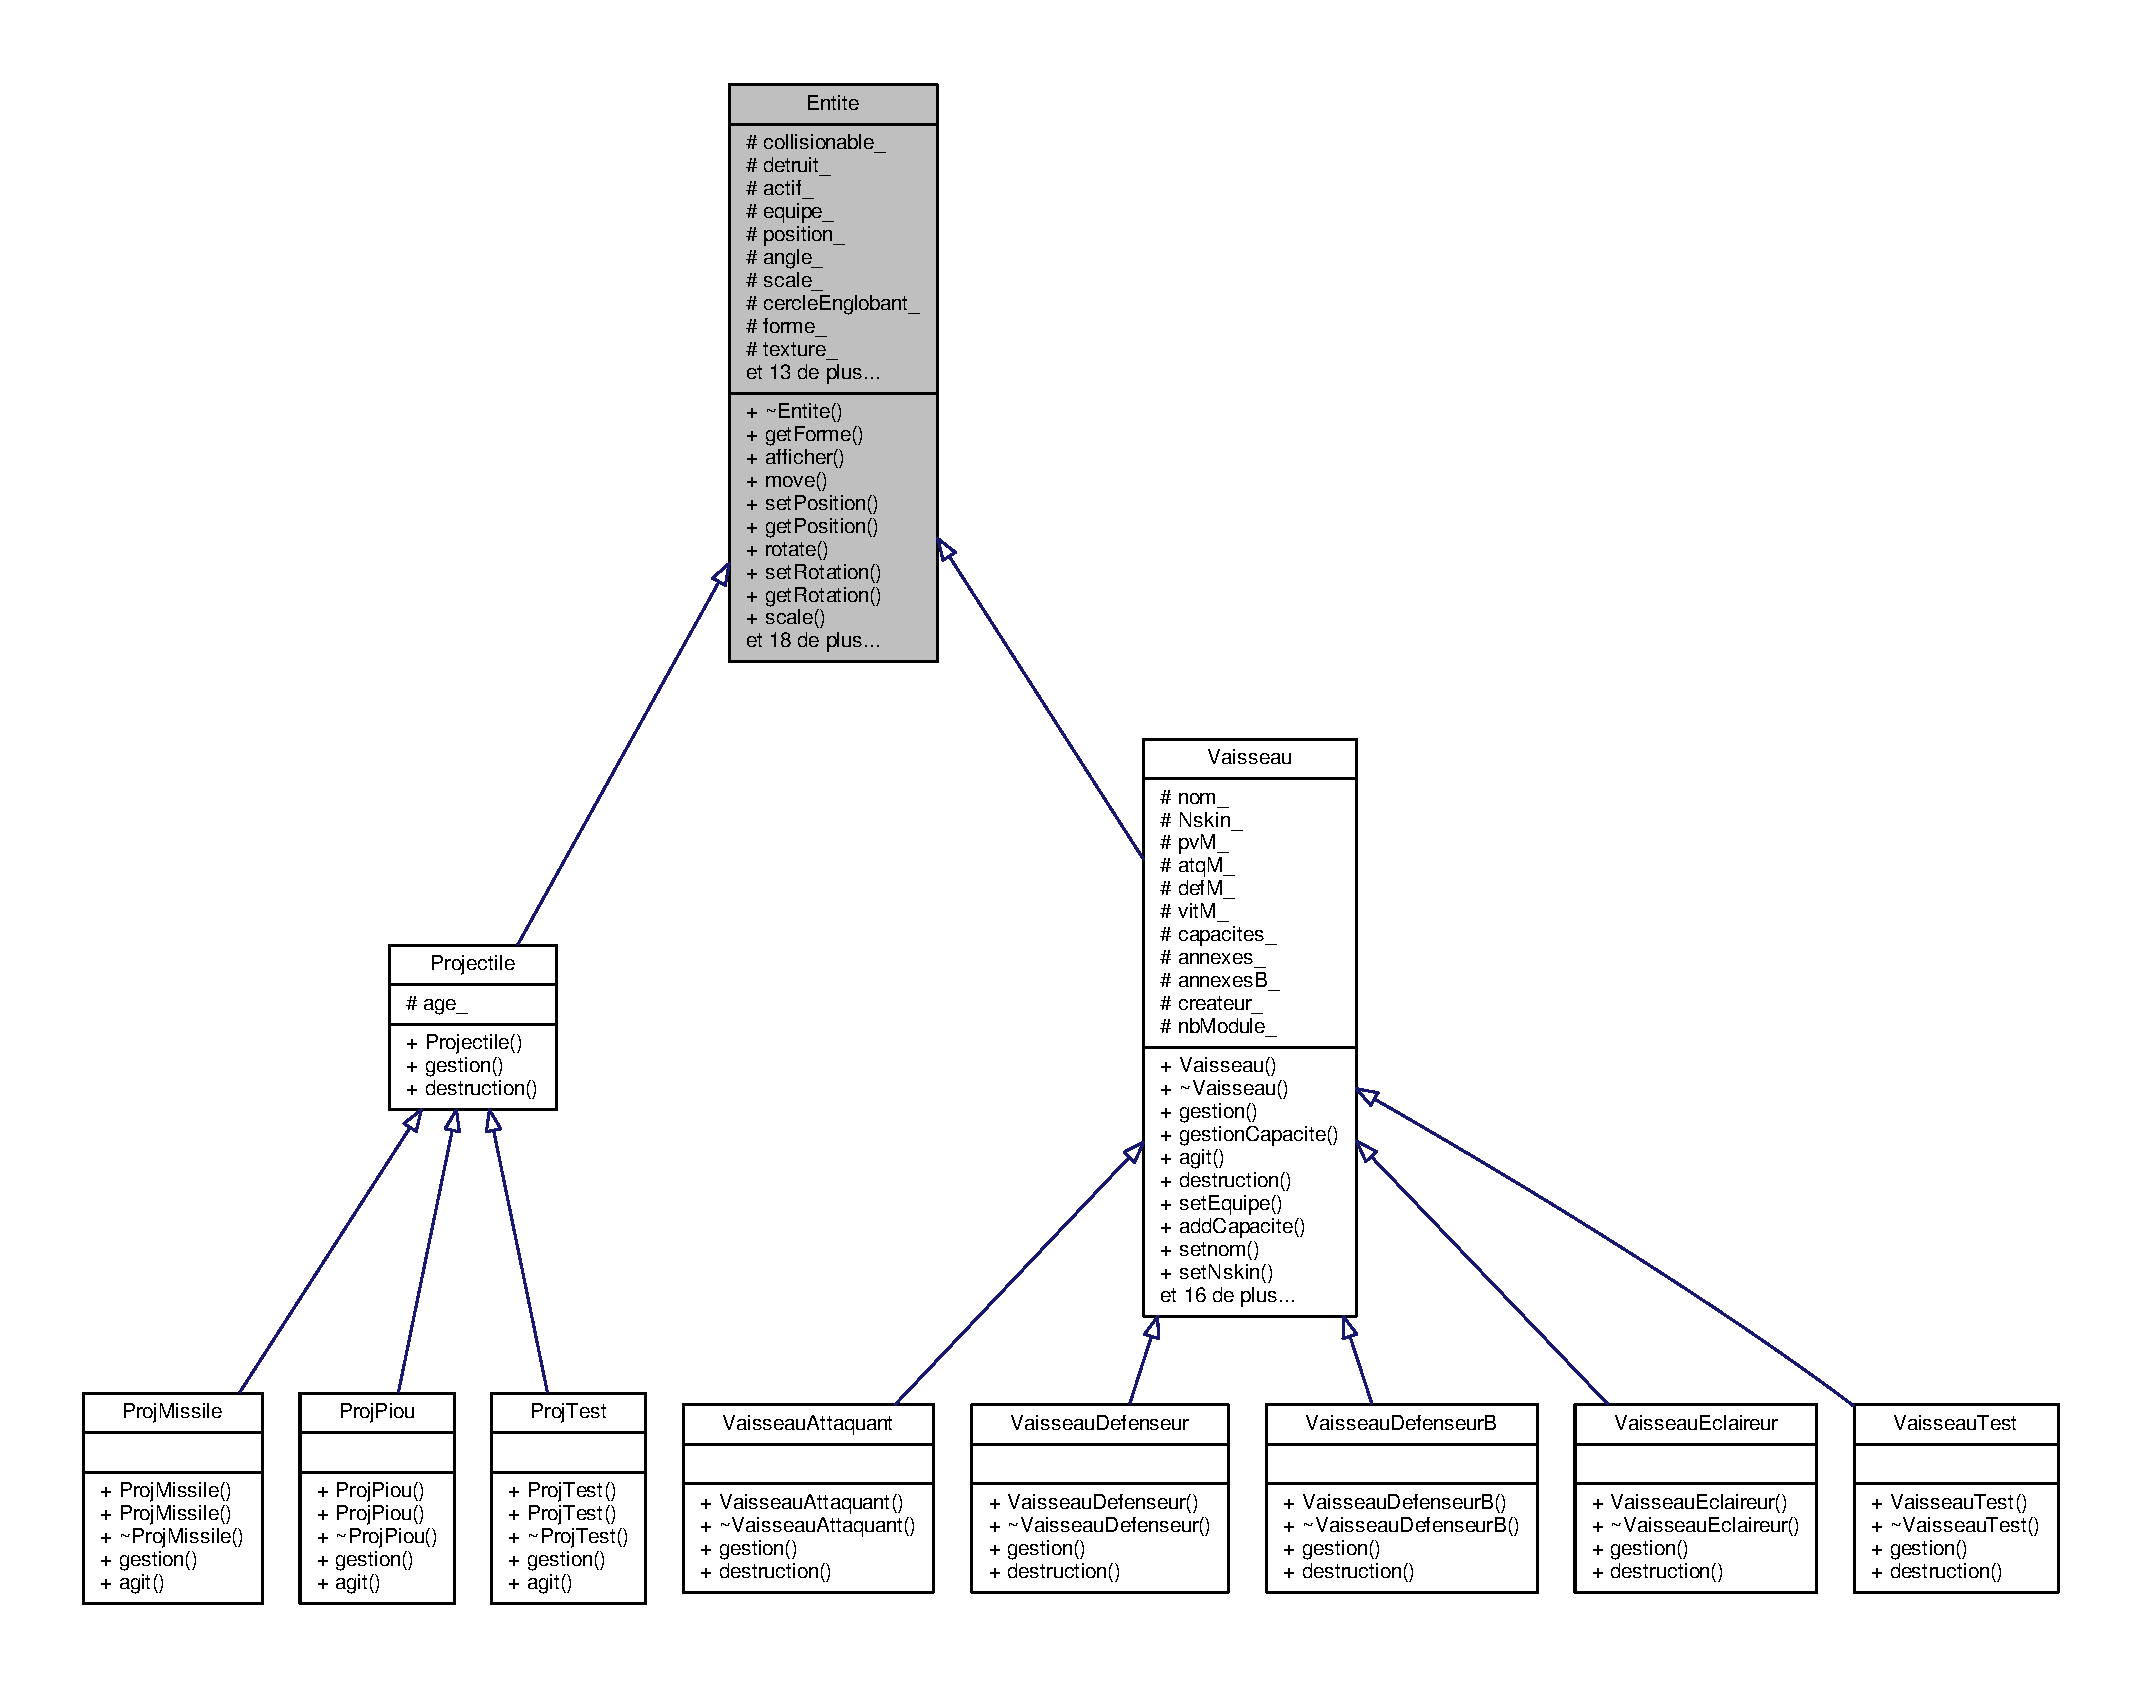
\includegraphics[width=299pt]{class_entite__inherit__graph}
\end{center}
\end{figure}
\subsection*{Fonctions membres publiques}
\begin{DoxyCompactItemize}
\item 
virtual \hyperlink{class_entite_a8084762a25afbfbcdca31121a3dfcd87}{$\sim$\+Entite} ()=default
\begin{DoxyCompactList}\small\item\em Destructeur par défaut. \end{DoxyCompactList}\item 
const std\+::vector$<$ std\+::unique\+\_\+ptr$<$ sf\+::\+Shape $>$ $>$ \& \hyperlink{class_entite_ae01177a102251100c96e2060372627ad}{get\+Forme} () const
\item 
void \hyperlink{class_entite_a91874d7e87f6cb479a3893fbedc6a4e3}{afficher} (sf\+::\+Render\+Window \&window, bool debug=false) const
\begin{DoxyCompactList}\small\item\em Affiche le sprite de l\textquotesingle{}\hyperlink{class_entite}{Entite}. \end{DoxyCompactList}\item 
void \hyperlink{class_entite_ac409613f3cf67cae14babd4b16811c8f}{move} (const sf\+::\+Vector2f \&delta)
\begin{DoxyCompactList}\small\item\em Déplace l\textquotesingle{}\hyperlink{class_entite}{Entite} en fonction de {\itshape delta}. \end{DoxyCompactList}\item 
void \hyperlink{class_entite_aa7fe4a7ebd8eb4c80ef9fdb7d97f2dad}{set\+Position} (const sf\+::\+Vector2f \&pos)
\begin{DoxyCompactList}\small\item\em Fixe la position de l\textquotesingle{}\hyperlink{class_entite}{Entite}. \end{DoxyCompactList}\item 
const sf\+::\+Vector2f \& \hyperlink{class_entite_a6f6fd1e1f9f6ad44f0ecc74961a774d9}{get\+Position} () const
\begin{DoxyCompactList}\small\item\em Renvoie la position de l\textquotesingle{}\hyperlink{class_entite}{Entite} appelante. \end{DoxyCompactList}\item 
void \hyperlink{class_entite_af1249039d313e4e691a109440663eae7}{rotate} (float angle)
\begin{DoxyCompactList}\small\item\em Tourne l\textquotesingle{}\hyperlink{class_entite}{Entite} de l\textquotesingle{}angle passé en paramètre. \end{DoxyCompactList}\item 
void \hyperlink{class_entite_a8623ac815e34b553098f45696ea8918b}{set\+Rotation} (float angle)
\begin{DoxyCompactList}\small\item\em Fixe l\textquotesingle{}orientation de l\textquotesingle{}\hyperlink{class_entite}{Entite} appelante. \end{DoxyCompactList}\item 
float \hyperlink{class_entite_a7f19439f7e7a5028f4b26eff21683de9}{get\+Rotation} () const
\begin{DoxyCompactList}\small\item\em Récupère l\textquotesingle{}orientation de l\textquotesingle{}\hyperlink{class_entite}{Entite}. \end{DoxyCompactList}\item 
void \hyperlink{class_entite_a770f6c53856606c4de768bb942299659}{scale} (float factor)
\begin{DoxyCompactList}\small\item\em Change l\textquotesingle{}échelle de l\textquotesingle{}\hyperlink{class_entite}{Entite}. \end{DoxyCompactList}\item 
void \hyperlink{class_entite_a665939253829baba965ce3ead0f1739c}{set\+Scale} (float factor)
\begin{DoxyCompactList}\small\item\em Fixe l\textquotesingle{}échelle de L\textquotesingle{}entite. \end{DoxyCompactList}\item 
float \hyperlink{class_entite_a5f70868f62049291edf4b245a531a6e0}{get\+Scale} () const
\begin{DoxyCompactList}\small\item\em Renvoie l\textquotesingle{}échelle de l\textquotesingle{}\hyperlink{class_entite}{Entite}. \end{DoxyCompactList}\item 
bool \hyperlink{class_entite_a8734ec47c87feb2b8b221bbf5d9ff2b4}{est\+Dehors} () const
\item 
void \hyperlink{class_entite_a88c148848289e34ca3bc991c37db9b44}{change\+Speed} (int val)
\end{DoxyCompactItemize}
\subsection*{Attributs protégés}
\begin{DoxyCompactItemize}
\item 
bool \hyperlink{class_entite_a37bb9bd568e9e1c904eaa83ec49a2b16}{collisionable\+\_\+} = true
\begin{DoxyCompactList}\small\item\em Booléen vrai si collisionnable. \end{DoxyCompactList}\item 
int \hyperlink{class_entite_a86f42758a3e4672052331b7a4daa10b5}{equipe\+\_\+}
\begin{DoxyCompactList}\small\item\em numéro d\textquotesingle{}équipe \end{DoxyCompactList}\item 
sf\+::\+Vector2f \hyperlink{class_entite_abbd554c4f122159a73cb113cc8de3860}{position\+\_\+}
\item 
float \hyperlink{class_entite_a2d6dc6bfcee492337b7422f12b393141}{angle\+\_\+}
\item 
float \hyperlink{class_entite_a50e0f8c1188d9833432c55c7f7d2aa0f}{scale\+\_\+}
\item 
sf\+::\+Circle\+Shape \hyperlink{class_entite_a5b6c62e4dc54221a84ce4dc824fdb2da}{cercle\+Englobant\+\_\+}
\item 
std\+::vector$<$ std\+::unique\+\_\+ptr$<$ sf\+::\+Shape $>$ $>$ \hyperlink{class_entite_aa6bbda9a40f701f273c344406a6f5122}{forme\+\_\+}
\item 
sf\+::\+Texture \hyperlink{class_entite_a8147b9459318a9b1de1b72dce115680a}{texture\+\_\+}
\item 
sf\+::\+Sprite \hyperlink{class_entite_ab7c03b6fe5c4f1d08cd3e4304e0ef7c0}{sprite\+\_\+}
\item 
int \hyperlink{class_entite_a62c3145096f707457d60306ea6729ed6}{vit\+\_\+}
\begin{DoxyCompactList}\small\item\em Vitesse actuelle. \end{DoxyCompactList}\end{DoxyCompactItemize}
\subsection*{Amis}
\begin{DoxyCompactItemize}
\item 
bool \hyperlink{class_entite_ac5011435e5099909dd34cd1750933b30}{collision} (const \hyperlink{class_entite}{Entite} \&e1, const \hyperlink{class_entite}{Entite} \&e2)
\begin{DoxyCompactList}\small\item\em Détecte une collision entre deux \hyperlink{class_entite}{Entite}. \end{DoxyCompactList}\end{DoxyCompactItemize}


\subsection{Description détaillée}
Classe virtuelle qui définit une entité 

Cette classe est une base à toutes les entités du jeu, les vaisseaux et les projectiles. Elle définit l\textquotesingle{}interface globale à travers laquelle ces entités peuvent être manipulées 

\subsection{Documentation des constructeurs et destructeur}
\mbox{\Hypertarget{class_entite_a8084762a25afbfbcdca31121a3dfcd87}\label{class_entite_a8084762a25afbfbcdca31121a3dfcd87}} 
\index{Entite@{Entite}!````~Entite@{$\sim$\+Entite}}
\index{````~Entite@{$\sim$\+Entite}!Entite@{Entite}}
\subsubsection{\texorpdfstring{$\sim$\+Entite()}{~Entite()}}
{\footnotesize\ttfamily Entite\+::$\sim$\+Entite (\begin{DoxyParamCaption}{ }\end{DoxyParamCaption})\hspace{0.3cm}{\ttfamily [virtual]}, {\ttfamily [default]}}



Destructeur par défaut. 

Destructeur virtuel par défaut de la classe \hyperlink{class_entite}{Entite}. Le destructeur est virtuel car la classe a vocation à être héritée. Il n\textquotesingle{}y a rien de spécial à faire donc le destructeur par défaut convient 

\subsection{Documentation des fonctions membres}
\mbox{\Hypertarget{class_entite_a91874d7e87f6cb479a3893fbedc6a4e3}\label{class_entite_a91874d7e87f6cb479a3893fbedc6a4e3}} 
\index{Entite@{Entite}!afficher@{afficher}}
\index{afficher@{afficher}!Entite@{Entite}}
\subsubsection{\texorpdfstring{afficher()}{afficher()}}
{\footnotesize\ttfamily Entite\+::afficher (\begin{DoxyParamCaption}\item[{sf\+::\+Render\+Window \&}]{window,  }\item[{bool}]{debug = {\ttfamily false} }\end{DoxyParamCaption}) const}



Affiche le sprite de l\textquotesingle{}\hyperlink{class_entite}{Entite}. 

Appelle la fonction afficher de la S\+F\+ML sur les attributs de l\textquotesingle{}objet appelant. Peut également afficher des informations de debug telles que le cercle englobant, et la forme de collision. 
\begin{DoxyParams}[1]{Paramètres}
\mbox{\tt in,out}  & {\em window} & Fenêtre S\+F\+ML dans laquelle afficher l\textquotesingle{}entité. \\
\hline
\mbox{\tt in}  & {\em debug} & Un {\ttfamily bool} qui vaut {\itshape true} si les informations de debug doivent être affichées et {\itshape false} sinon. \\
\hline
\end{DoxyParams}
\mbox{\Hypertarget{class_entite_a88c148848289e34ca3bc991c37db9b44}\label{class_entite_a88c148848289e34ca3bc991c37db9b44}} 
\index{Entite@{Entite}!change\+Speed@{change\+Speed}}
\index{change\+Speed@{change\+Speed}!Entite@{Entite}}
\subsubsection{\texorpdfstring{change\+Speed()}{changeSpeed()}}
{\footnotesize\ttfamily void Entite\+::change\+Speed (\begin{DoxyParamCaption}\item[{int}]{val }\end{DoxyParamCaption})}

\mbox{\Hypertarget{class_entite_a8734ec47c87feb2b8b221bbf5d9ff2b4}\label{class_entite_a8734ec47c87feb2b8b221bbf5d9ff2b4}} 
\index{Entite@{Entite}!est\+Dehors@{est\+Dehors}}
\index{est\+Dehors@{est\+Dehors}!Entite@{Entite}}
\subsubsection{\texorpdfstring{est\+Dehors()}{estDehors()}}
{\footnotesize\ttfamily bool Entite\+::est\+Dehors (\begin{DoxyParamCaption}{ }\end{DoxyParamCaption}) const}

\mbox{\Hypertarget{class_entite_ae01177a102251100c96e2060372627ad}\label{class_entite_ae01177a102251100c96e2060372627ad}} 
\index{Entite@{Entite}!get\+Forme@{get\+Forme}}
\index{get\+Forme@{get\+Forme}!Entite@{Entite}}
\subsubsection{\texorpdfstring{get\+Forme()}{getForme()}}
{\footnotesize\ttfamily const std\+::vector$<$std\+::unique\+\_\+ptr$<$sf\+::\+Shape$>$ $>$\& Entite\+::get\+Forme (\begin{DoxyParamCaption}{ }\end{DoxyParamCaption}) const\hspace{0.3cm}{\ttfamily [inline]}}

\mbox{\Hypertarget{class_entite_a6f6fd1e1f9f6ad44f0ecc74961a774d9}\label{class_entite_a6f6fd1e1f9f6ad44f0ecc74961a774d9}} 
\index{Entite@{Entite}!get\+Position@{get\+Position}}
\index{get\+Position@{get\+Position}!Entite@{Entite}}
\subsubsection{\texorpdfstring{get\+Position()}{getPosition()}}
{\footnotesize\ttfamily Entite\+::get\+Position (\begin{DoxyParamCaption}{ }\end{DoxyParamCaption}) const}



Renvoie la position de l\textquotesingle{}\hyperlink{class_entite}{Entite} appelante. 

Cette fonction renvoie la position actuelle de l\textquotesingle{}\hyperlink{class_entite}{Entite} appelante par rapport au point haut gauche de la fenêtre \begin{DoxyReturn}{Renvoie}
la position de l\textquotesingle{}entité appelante 
\end{DoxyReturn}
\mbox{\Hypertarget{class_entite_a7f19439f7e7a5028f4b26eff21683de9}\label{class_entite_a7f19439f7e7a5028f4b26eff21683de9}} 
\index{Entite@{Entite}!get\+Rotation@{get\+Rotation}}
\index{get\+Rotation@{get\+Rotation}!Entite@{Entite}}
\subsubsection{\texorpdfstring{get\+Rotation()}{getRotation()}}
{\footnotesize\ttfamily Entite\+::get\+Rotation (\begin{DoxyParamCaption}{ }\end{DoxyParamCaption}) const}



Récupère l\textquotesingle{}orientation de l\textquotesingle{}\hyperlink{class_entite}{Entite}. 

Cette fonction renvoie l\textquotesingle{}orientation actuelle de l\textquotesingle{}\hyperlink{class_entite}{Entite} appelante. La valeur renvoyée correspond à un angle en degrés \begin{DoxyReturn}{Renvoie}
Un {\ttfamily float} qui correspond à l\textquotesingle{}eorientation de l\textquotesingle{}\hyperlink{class_entite}{Entite} 
\end{DoxyReturn}
\mbox{\Hypertarget{class_entite_a5f70868f62049291edf4b245a531a6e0}\label{class_entite_a5f70868f62049291edf4b245a531a6e0}} 
\index{Entite@{Entite}!get\+Scale@{get\+Scale}}
\index{get\+Scale@{get\+Scale}!Entite@{Entite}}
\subsubsection{\texorpdfstring{get\+Scale()}{getScale()}}
{\footnotesize\ttfamily Entite\+::get\+Scale (\begin{DoxyParamCaption}{ }\end{DoxyParamCaption}) const}



Renvoie l\textquotesingle{}échelle de l\textquotesingle{}\hyperlink{class_entite}{Entite}. 

Cette fonction renvoie l\textquotesingle{}échelle actuelle de l\textquotesingle{}\hyperlink{class_entite}{Entite} appelante \begin{DoxyReturn}{Renvoie}
Un {\ttfamily float} qui correspond au facteur d\textquotesingle{}échelle de l\textquotesingle{}\hyperlink{class_entite}{Entite} 
\end{DoxyReturn}
\mbox{\Hypertarget{class_entite_ac409613f3cf67cae14babd4b16811c8f}\label{class_entite_ac409613f3cf67cae14babd4b16811c8f}} 
\index{Entite@{Entite}!move@{move}}
\index{move@{move}!Entite@{Entite}}
\subsubsection{\texorpdfstring{move()}{move()}}
{\footnotesize\ttfamily Entite\+::move (\begin{DoxyParamCaption}\item[{const sf\+::\+Vector2f \&}]{delta }\end{DoxyParamCaption})}



Déplace l\textquotesingle{}\hyperlink{class_entite}{Entite} en fonction de {\itshape delta}. 

Appelle la fonction move de la S\+F\+ML sur les attributs de l\textquotesingle{}objet appelant. 
\begin{DoxyParams}[1]{Paramètres}
\mbox{\tt in}  & {\em delta} & un {\ttfamily sf\+::\+Vector2f} qui donne le déplacement en x et en y \\
\hline
\end{DoxyParams}
\mbox{\Hypertarget{class_entite_af1249039d313e4e691a109440663eae7}\label{class_entite_af1249039d313e4e691a109440663eae7}} 
\index{Entite@{Entite}!rotate@{rotate}}
\index{rotate@{rotate}!Entite@{Entite}}
\subsubsection{\texorpdfstring{rotate()}{rotate()}}
{\footnotesize\ttfamily Entite\+::rotate (\begin{DoxyParamCaption}\item[{float}]{angle }\end{DoxyParamCaption})}



Tourne l\textquotesingle{}\hyperlink{class_entite}{Entite} de l\textquotesingle{}angle passé en paramètre. 

Cette fonction permet de aire tourner l\textquotesingle{}entité de l\textquotesingle{}angle passé en paramètre, chaque élément composant l\textquotesingle{}entité est tourné. L\textquotesingle{}angle est donné en degrés 
\begin{DoxyParams}[1]{Paramètres}
\mbox{\tt in}  & {\em angle} & \\
\hline
\end{DoxyParams}
\mbox{\Hypertarget{class_entite_a770f6c53856606c4de768bb942299659}\label{class_entite_a770f6c53856606c4de768bb942299659}} 
\index{Entite@{Entite}!scale@{scale}}
\index{scale@{scale}!Entite@{Entite}}
\subsubsection{\texorpdfstring{scale()}{scale()}}
{\footnotesize\ttfamily Entite\+::scale (\begin{DoxyParamCaption}\item[{float}]{factor }\end{DoxyParamCaption})}



Change l\textquotesingle{}échelle de l\textquotesingle{}\hyperlink{class_entite}{Entite}. 

Cette fonction permet de modifier l\textquotesingle{}échelle de l\textquotesingle{}\hyperlink{class_entite}{Entite} appelante en appliquant un coefficient multiplicateur à ses dimensions. Un coefficient de 0.\+5 divisera les dimentions par 2, à l\textquotesingle{}inverse un coefficient de 2 rendra l\textquotesingle{}\hyperlink{class_entite}{Entite} 2 fois plus grande. Un coefficient de 1 ne changera rien. 
\begin{DoxyParams}[1]{Paramètres}
\mbox{\tt in}  & {\em factor} & Le coefficient multiplicateur d\textquotesingle{}échelle à appliquer \\
\hline
\end{DoxyParams}
\mbox{\Hypertarget{class_entite_aa7fe4a7ebd8eb4c80ef9fdb7d97f2dad}\label{class_entite_aa7fe4a7ebd8eb4c80ef9fdb7d97f2dad}} 
\index{Entite@{Entite}!set\+Position@{set\+Position}}
\index{set\+Position@{set\+Position}!Entite@{Entite}}
\subsubsection{\texorpdfstring{set\+Position()}{setPosition()}}
{\footnotesize\ttfamily Entite\+::set\+Position (\begin{DoxyParamCaption}\item[{const sf\+::\+Vector2f \&}]{pos }\end{DoxyParamCaption})}



Fixe la position de l\textquotesingle{}\hyperlink{class_entite}{Entite}. 

Cette fonction change la position de l\textquotesingle{}\hyperlink{class_entite}{Entite} appelante avec les coordonnées données en paramètres. Ces coordonnées sont relatives au coin supérieur gauche de la fenêtre. Cette fonction est implémentée à partir de la fonction {\itshape move} afin que chaque élément reste au même endroit par rapport aux autres s\textquotesingle{}il n\textquotesingle{}ont pas la même position initiale. 
\begin{DoxyParams}[1]{Paramètres}
\mbox{\tt in}  & {\em pos} & Un {\ttfamily sf\+::\+Vector2f} qui contient la nouvelle position \\
\hline
\end{DoxyParams}
\mbox{\Hypertarget{class_entite_a8623ac815e34b553098f45696ea8918b}\label{class_entite_a8623ac815e34b553098f45696ea8918b}} 
\index{Entite@{Entite}!set\+Rotation@{set\+Rotation}}
\index{set\+Rotation@{set\+Rotation}!Entite@{Entite}}
\subsubsection{\texorpdfstring{set\+Rotation()}{setRotation()}}
{\footnotesize\ttfamily Entite\+::set\+Rotation (\begin{DoxyParamCaption}\item[{float}]{angle }\end{DoxyParamCaption})}



Fixe l\textquotesingle{}orientation de l\textquotesingle{}\hyperlink{class_entite}{Entite} appelante. 

Cette fonction change l\textquotesingle{}orientation de l\textquotesingle{}\hyperlink{class_entite}{Entite} appelante à l\textquotesingle{}angle passé en paramètres. La valeur de l\textquotesingle{}angle est donnée en degrés. Cette fonction est implémentée en utilisant la fonction rotate pour que les éléments ne soient pa décalés les uns par rapport aux autres s\textquotesingle{}ils ne disposent pas de la même orientation initiale. 
\begin{DoxyParams}[1]{Paramètres}
\mbox{\tt in}  & {\em angle} & La nouvelle orientation de l\textquotesingle{}\hyperlink{class_entite}{Entite} \\
\hline
\end{DoxyParams}
\mbox{\Hypertarget{class_entite_a665939253829baba965ce3ead0f1739c}\label{class_entite_a665939253829baba965ce3ead0f1739c}} 
\index{Entite@{Entite}!set\+Scale@{set\+Scale}}
\index{set\+Scale@{set\+Scale}!Entite@{Entite}}
\subsubsection{\texorpdfstring{set\+Scale()}{setScale()}}
{\footnotesize\ttfamily Entite\+::set\+Scale (\begin{DoxyParamCaption}\item[{float}]{factor }\end{DoxyParamCaption})}



Fixe l\textquotesingle{}échelle de L\textquotesingle{}entite. 

Cette fonction permet de fixer l\textquotesingle{}échelle de L\textquotesingle{}entite appelante. Contrairement à la fonction scale, cette fonction fixe l\textquotesingle{}échelle de manière absolue et non relativement au changements d\textquotesingle{}échelle déjà appliqué à l\textquotesingle{}\hyperlink{class_entite}{Entite} 
\begin{DoxyParams}[1]{Paramètres}
\mbox{\tt in}  & {\em factor} & Le facteur d\textquotesingle{}échelle à appliquer \\
\hline
\end{DoxyParams}


\subsection{Documentation des fonctions amies et associées}
\mbox{\Hypertarget{class_entite_ac5011435e5099909dd34cd1750933b30}\label{class_entite_ac5011435e5099909dd34cd1750933b30}} 
\index{Entite@{Entite}!collision@{collision}}
\index{collision@{collision}!Entite@{Entite}}
\subsubsection{\texorpdfstring{collision}{collision}}
{\footnotesize\ttfamily Entite\+::collision (\begin{DoxyParamCaption}\item[{const \hyperlink{class_entite}{Entite} \&}]{e1,  }\item[{const \hyperlink{class_entite}{Entite} \&}]{e2 }\end{DoxyParamCaption})\hspace{0.3cm}{\ttfamily [friend]}}



Détecte une collision entre deux \hyperlink{class_entite}{Entite}. 

Cette fonction permet de détecter si deux \hyperlink{class_entite}{Entite} sont en collision ou non. Cette fonction prend en compte si les deux \hyperlink{class_entite}{Entite} sont collisionables, si elles sont d\textquotesingle{}équipes différentes, si leur cercles englobants sont en collision et finalement si leur formes de collisions sont en collision 
\begin{DoxyParams}[1]{Paramètres}
\mbox{\tt in}  & {\em e1} & La première \hyperlink{class_entite}{Entite} à tester \\
\hline
\mbox{\tt in}  & {\em e2} & La deuxième \hyperlink{class_entite}{Entite} à tester \\
\hline
\end{DoxyParams}
\begin{DoxyReturn}{Renvoie}
Un {\ttfamily bool} qui vaut {\itshape true} si les \hyperlink{class_entite}{Entite} sont en collision et {\itshape false} sinon 
\end{DoxyReturn}


\subsection{Documentation des données membres}
\mbox{\Hypertarget{class_entite_a2d6dc6bfcee492337b7422f12b393141}\label{class_entite_a2d6dc6bfcee492337b7422f12b393141}} 
\index{Entite@{Entite}!angle\+\_\+@{angle\+\_\+}}
\index{angle\+\_\+@{angle\+\_\+}!Entite@{Entite}}
\subsubsection{\texorpdfstring{angle\+\_\+}{angle\_}}
{\footnotesize\ttfamily float Entite\+::angle\+\_\+\hspace{0.3cm}{\ttfamily [protected]}}

\mbox{\Hypertarget{class_entite_a5b6c62e4dc54221a84ce4dc824fdb2da}\label{class_entite_a5b6c62e4dc54221a84ce4dc824fdb2da}} 
\index{Entite@{Entite}!cercle\+Englobant\+\_\+@{cercle\+Englobant\+\_\+}}
\index{cercle\+Englobant\+\_\+@{cercle\+Englobant\+\_\+}!Entite@{Entite}}
\subsubsection{\texorpdfstring{cercle\+Englobant\+\_\+}{cercleEnglobant\_}}
{\footnotesize\ttfamily sf\+::\+Circle\+Shape Entite\+::cercle\+Englobant\+\_\+\hspace{0.3cm}{\ttfamily [protected]}}

\mbox{\Hypertarget{class_entite_a37bb9bd568e9e1c904eaa83ec49a2b16}\label{class_entite_a37bb9bd568e9e1c904eaa83ec49a2b16}} 
\index{Entite@{Entite}!collisionable\+\_\+@{collisionable\+\_\+}}
\index{collisionable\+\_\+@{collisionable\+\_\+}!Entite@{Entite}}
\subsubsection{\texorpdfstring{collisionable\+\_\+}{collisionable\_}}
{\footnotesize\ttfamily bool Entite\+::collisionable\+\_\+ = true\hspace{0.3cm}{\ttfamily [protected]}}



Booléen vrai si collisionnable. 

\mbox{\Hypertarget{class_entite_a86f42758a3e4672052331b7a4daa10b5}\label{class_entite_a86f42758a3e4672052331b7a4daa10b5}} 
\index{Entite@{Entite}!equipe\+\_\+@{equipe\+\_\+}}
\index{equipe\+\_\+@{equipe\+\_\+}!Entite@{Entite}}
\subsubsection{\texorpdfstring{equipe\+\_\+}{equipe\_}}
{\footnotesize\ttfamily int Entite\+::equipe\+\_\+\hspace{0.3cm}{\ttfamily [protected]}}



numéro d\textquotesingle{}équipe 

\mbox{\Hypertarget{class_entite_aa6bbda9a40f701f273c344406a6f5122}\label{class_entite_aa6bbda9a40f701f273c344406a6f5122}} 
\index{Entite@{Entite}!forme\+\_\+@{forme\+\_\+}}
\index{forme\+\_\+@{forme\+\_\+}!Entite@{Entite}}
\subsubsection{\texorpdfstring{forme\+\_\+}{forme\_}}
{\footnotesize\ttfamily std\+::vector$<$std\+::unique\+\_\+ptr$<$sf\+::\+Shape$>$ $>$ Entite\+::forme\+\_\+\hspace{0.3cm}{\ttfamily [protected]}}

\mbox{\Hypertarget{class_entite_abbd554c4f122159a73cb113cc8de3860}\label{class_entite_abbd554c4f122159a73cb113cc8de3860}} 
\index{Entite@{Entite}!position\+\_\+@{position\+\_\+}}
\index{position\+\_\+@{position\+\_\+}!Entite@{Entite}}
\subsubsection{\texorpdfstring{position\+\_\+}{position\_}}
{\footnotesize\ttfamily sf\+::\+Vector2f Entite\+::position\+\_\+\hspace{0.3cm}{\ttfamily [protected]}}

\mbox{\Hypertarget{class_entite_a50e0f8c1188d9833432c55c7f7d2aa0f}\label{class_entite_a50e0f8c1188d9833432c55c7f7d2aa0f}} 
\index{Entite@{Entite}!scale\+\_\+@{scale\+\_\+}}
\index{scale\+\_\+@{scale\+\_\+}!Entite@{Entite}}
\subsubsection{\texorpdfstring{scale\+\_\+}{scale\_}}
{\footnotesize\ttfamily float Entite\+::scale\+\_\+\hspace{0.3cm}{\ttfamily [protected]}}

\mbox{\Hypertarget{class_entite_ab7c03b6fe5c4f1d08cd3e4304e0ef7c0}\label{class_entite_ab7c03b6fe5c4f1d08cd3e4304e0ef7c0}} 
\index{Entite@{Entite}!sprite\+\_\+@{sprite\+\_\+}}
\index{sprite\+\_\+@{sprite\+\_\+}!Entite@{Entite}}
\subsubsection{\texorpdfstring{sprite\+\_\+}{sprite\_}}
{\footnotesize\ttfamily sf\+::\+Sprite Entite\+::sprite\+\_\+\hspace{0.3cm}{\ttfamily [protected]}}

\mbox{\Hypertarget{class_entite_a8147b9459318a9b1de1b72dce115680a}\label{class_entite_a8147b9459318a9b1de1b72dce115680a}} 
\index{Entite@{Entite}!texture\+\_\+@{texture\+\_\+}}
\index{texture\+\_\+@{texture\+\_\+}!Entite@{Entite}}
\subsubsection{\texorpdfstring{texture\+\_\+}{texture\_}}
{\footnotesize\ttfamily sf\+::\+Texture Entite\+::texture\+\_\+\hspace{0.3cm}{\ttfamily [protected]}}

\mbox{\Hypertarget{class_entite_a62c3145096f707457d60306ea6729ed6}\label{class_entite_a62c3145096f707457d60306ea6729ed6}} 
\index{Entite@{Entite}!vit\+\_\+@{vit\+\_\+}}
\index{vit\+\_\+@{vit\+\_\+}!Entite@{Entite}}
\subsubsection{\texorpdfstring{vit\+\_\+}{vit\_}}
{\footnotesize\ttfamily int Entite\+::vit\+\_\+\hspace{0.3cm}{\ttfamily [protected]}}



Vitesse actuelle. 



La documentation de cette classe a été générée à partir des fichiers suivants \+:\begin{DoxyCompactItemize}
\item 
src/\hyperlink{_entite_8h}{Entite.\+h}\item 
src/\hyperlink{_entite_8cpp}{Entite.\+cpp}\end{DoxyCompactItemize}

\hypertarget{structstd_1_1experimental_1_1is__nothrow__move__assignable_1_1has__nothrow__move__assign}{}\section{Référence du modèle de la structure std\+:\+:experimental\+:\+:is\+\_\+nothrow\+\_\+move\+\_\+assignable$<$ T $>$\+:\+:has\+\_\+nothrow\+\_\+move\+\_\+assign$<$ X, has\+\_\+any\+\_\+move\+\_\+assign $>$}
\label{structstd_1_1experimental_1_1is__nothrow__move__assignable_1_1has__nothrow__move__assign}\index{std\+::experimental\+::is\+\_\+nothrow\+\_\+move\+\_\+assignable$<$ T $>$\+::has\+\_\+nothrow\+\_\+move\+\_\+assign$<$ X, has\+\_\+any\+\_\+move\+\_\+assign $>$@{std\+::experimental\+::is\+\_\+nothrow\+\_\+move\+\_\+assignable$<$ T $>$\+::has\+\_\+nothrow\+\_\+move\+\_\+assign$<$ X, has\+\_\+any\+\_\+move\+\_\+assign $>$}}


{\ttfamily \#include $<$optional.\+h$>$}



Graphe de collaboration de std\+:\+:experimental\+:\+:is\+\_\+nothrow\+\_\+move\+\_\+assignable$<$ T $>$\+:\+:has\+\_\+nothrow\+\_\+move\+\_\+assign$<$ X, has\+\_\+any\+\_\+move\+\_\+assign $>$\+:
% FIG 0
\subsection*{Attributs publics statiques}
\begin{DoxyCompactItemize}
\item 
static constexpr bool \hyperlink{structstd_1_1experimental_1_1is__nothrow__move__assignable_1_1has__nothrow__move__assign_a532e5e86417df21c93d054170894071d}{value} = false
\end{DoxyCompactItemize}


\subsection{Documentation des données membres}
\mbox{\Hypertarget{structstd_1_1experimental_1_1is__nothrow__move__assignable_1_1has__nothrow__move__assign_a532e5e86417df21c93d054170894071d}\label{structstd_1_1experimental_1_1is__nothrow__move__assignable_1_1has__nothrow__move__assign_a532e5e86417df21c93d054170894071d}} 
\index{std\+::experimental\+::is\+\_\+nothrow\+\_\+move\+\_\+assignable\+::has\+\_\+nothrow\+\_\+move\+\_\+assign@{std\+::experimental\+::is\+\_\+nothrow\+\_\+move\+\_\+assignable\+::has\+\_\+nothrow\+\_\+move\+\_\+assign}!value@{value}}
\index{value@{value}!std\+::experimental\+::is\+\_\+nothrow\+\_\+move\+\_\+assignable\+::has\+\_\+nothrow\+\_\+move\+\_\+assign@{std\+::experimental\+::is\+\_\+nothrow\+\_\+move\+\_\+assignable\+::has\+\_\+nothrow\+\_\+move\+\_\+assign}}
\subsubsection{\texorpdfstring{value}{value}}
{\footnotesize\ttfamily template$<$class T $>$ \\
template$<$class X, bool has\+\_\+any\+\_\+move\+\_\+assign$>$ \\
constexpr bool \hyperlink{structstd_1_1experimental_1_1is__nothrow__move__assignable}{std\+::experimental\+::is\+\_\+nothrow\+\_\+move\+\_\+assignable}$<$ T $>$\+::\hyperlink{structstd_1_1experimental_1_1is__nothrow__move__assignable_1_1has__nothrow__move__assign}{has\+\_\+nothrow\+\_\+move\+\_\+assign}$<$ X, has\+\_\+any\+\_\+move\+\_\+assign $>$\+::value = false\hspace{0.3cm}{\ttfamily [static]}}



La documentation de cette structure a été générée à partir du fichier suivant \+:\begin{DoxyCompactItemize}
\item 
src/\+Utilitaires/\hyperlink{optional_8h}{optional.\+h}\end{DoxyCompactItemize}

\hypertarget{structstd_1_1experimental_1_1is__nothrow__move__assignable_1_1has__nothrow__move__assign_3_01_x_00_01true_01_4}{}\section{std\+:\+:experimental\+:\+:is\+\_\+nothrow\+\_\+move\+\_\+assignable$<$ T $>$\+:\+:has\+\_\+nothrow\+\_\+move\+\_\+assign$<$ X, true $>$ Struct Template Reference}
\label{structstd_1_1experimental_1_1is__nothrow__move__assignable_1_1has__nothrow__move__assign_3_01_x_00_01true_01_4}\index{std\+::experimental\+::is\+\_\+nothrow\+\_\+move\+\_\+assignable$<$ T $>$\+::has\+\_\+nothrow\+\_\+move\+\_\+assign$<$ X, true $>$@{std\+::experimental\+::is\+\_\+nothrow\+\_\+move\+\_\+assignable$<$ T $>$\+::has\+\_\+nothrow\+\_\+move\+\_\+assign$<$ X, true $>$}}


{\ttfamily \#include $<$optional.\+h$>$}

\subsection*{Static Public Attributes}
\begin{DoxyCompactItemize}
\item 
static constexpr bool \mbox{\hyperlink{structstd_1_1experimental_1_1is__nothrow__move__assignable_1_1has__nothrow__move__assign_3_01_x_00_01true_01_4_a94b7f221dd39c47cff4c6fa0dffaa4b4}{value}} = noexcept( std\+::declval$<$X\&$>$() = std\+::declval$<$X\&\&$>$() )
\end{DoxyCompactItemize}


\subsection{Member Data Documentation}
\mbox{\Hypertarget{structstd_1_1experimental_1_1is__nothrow__move__assignable_1_1has__nothrow__move__assign_3_01_x_00_01true_01_4_a94b7f221dd39c47cff4c6fa0dffaa4b4}\label{structstd_1_1experimental_1_1is__nothrow__move__assignable_1_1has__nothrow__move__assign_3_01_x_00_01true_01_4_a94b7f221dd39c47cff4c6fa0dffaa4b4}} 
\index{std\+::experimental\+::is\+\_\+nothrow\+\_\+move\+\_\+assignable\+::has\+\_\+nothrow\+\_\+move\+\_\+assign$<$ X, true $>$@{std\+::experimental\+::is\+\_\+nothrow\+\_\+move\+\_\+assignable\+::has\+\_\+nothrow\+\_\+move\+\_\+assign$<$ X, true $>$}!value@{value}}
\index{value@{value}!std\+::experimental\+::is\+\_\+nothrow\+\_\+move\+\_\+assignable\+::has\+\_\+nothrow\+\_\+move\+\_\+assign$<$ X, true $>$@{std\+::experimental\+::is\+\_\+nothrow\+\_\+move\+\_\+assignable\+::has\+\_\+nothrow\+\_\+move\+\_\+assign$<$ X, true $>$}}
\subsubsection{\texorpdfstring{value}{value}}
{\footnotesize\ttfamily template$<$class T $>$ \\
template$<$class X $>$ \\
constexpr bool \mbox{\hyperlink{structstd_1_1experimental_1_1is__nothrow__move__assignable}{std\+::experimental\+::is\+\_\+nothrow\+\_\+move\+\_\+assignable}}$<$ T $>$\+::\mbox{\hyperlink{structstd_1_1experimental_1_1is__nothrow__move__assignable_1_1has__nothrow__move__assign}{has\+\_\+nothrow\+\_\+move\+\_\+assign}}$<$ X, true $>$\+::value = noexcept( std\+::declval$<$X\&$>$() = std\+::declval$<$X\&\&$>$() )\hspace{0.3cm}{\ttfamily [static]}}



The documentation for this struct was generated from the following file\+:\begin{DoxyCompactItemize}
\item 
src/\+Utilitaires/\mbox{\hyperlink{optional_8h}{optional.\+h}}\end{DoxyCompactItemize}

\hypertarget{structstd_1_1experimental_1_1detail___1_1has__overloaded__addressof}{}\section{std\+:\+:experimental\+:\+:detail\+\_\+\+:\+:has\+\_\+overloaded\+\_\+addressof$<$ T $>$ Struct Template Reference}
\label{structstd_1_1experimental_1_1detail___1_1has__overloaded__addressof}\index{std\+::experimental\+::detail\+\_\+\+::has\+\_\+overloaded\+\_\+addressof$<$ T $>$@{std\+::experimental\+::detail\+\_\+\+::has\+\_\+overloaded\+\_\+addressof$<$ T $>$}}


{\ttfamily \#include $<$optional.\+h$>$}

\subsection*{Static Public Member Functions}
\begin{DoxyCompactItemize}
\item 
{\footnotesize template$<$class X $>$ }\\static constexpr bool \mbox{\hyperlink{structstd_1_1experimental_1_1detail___1_1has__overloaded__addressof_a4656eb4d63080eef6563dca4894f8623}{has\+\_\+overload}} (...)
\item 
{\footnotesize template$<$class X , size\+\_\+t S = sizeof(std\+::declval$<$\+X\&$>$().\+operator\&())$>$ }\\static constexpr bool \mbox{\hyperlink{structstd_1_1experimental_1_1detail___1_1has__overloaded__addressof_a3afc4b4cc2df22327c0f380cec60fb1f}{has\+\_\+overload}} (bool)
\end{DoxyCompactItemize}
\subsection*{Static Public Attributes}
\begin{DoxyCompactItemize}
\item 
static constexpr bool \mbox{\hyperlink{structstd_1_1experimental_1_1detail___1_1has__overloaded__addressof_a7ff16212ecdca54a0328b1cb4d676cf9}{value}} = \mbox{\hyperlink{structstd_1_1experimental_1_1detail___1_1has__overloaded__addressof_a4656eb4d63080eef6563dca4894f8623}{has\+\_\+overload}}$<$T$>$(true)
\end{DoxyCompactItemize}


\subsection{Member Function Documentation}
\mbox{\Hypertarget{structstd_1_1experimental_1_1detail___1_1has__overloaded__addressof_a4656eb4d63080eef6563dca4894f8623}\label{structstd_1_1experimental_1_1detail___1_1has__overloaded__addressof_a4656eb4d63080eef6563dca4894f8623}} 
\index{std\+::experimental\+::detail\+\_\+\+::has\+\_\+overloaded\+\_\+addressof@{std\+::experimental\+::detail\+\_\+\+::has\+\_\+overloaded\+\_\+addressof}!has\+\_\+overload@{has\+\_\+overload}}
\index{has\+\_\+overload@{has\+\_\+overload}!std\+::experimental\+::detail\+\_\+\+::has\+\_\+overloaded\+\_\+addressof@{std\+::experimental\+::detail\+\_\+\+::has\+\_\+overloaded\+\_\+addressof}}
\subsubsection{\texorpdfstring{has\+\_\+overload()}{has\_overload()}\hspace{0.1cm}{\footnotesize\ttfamily [1/2]}}
{\footnotesize\ttfamily template$<$typename T $>$ \\
template$<$class X $>$ \\
static constexpr bool \mbox{\hyperlink{structstd_1_1experimental_1_1detail___1_1has__overloaded__addressof}{std\+::experimental\+::detail\+\_\+\+::has\+\_\+overloaded\+\_\+addressof}}$<$ T $>$\+::has\+\_\+overload (\begin{DoxyParamCaption}\item[{}]{... }\end{DoxyParamCaption})\hspace{0.3cm}{\ttfamily [inline]}, {\ttfamily [static]}}

\mbox{\Hypertarget{structstd_1_1experimental_1_1detail___1_1has__overloaded__addressof_a3afc4b4cc2df22327c0f380cec60fb1f}\label{structstd_1_1experimental_1_1detail___1_1has__overloaded__addressof_a3afc4b4cc2df22327c0f380cec60fb1f}} 
\index{std\+::experimental\+::detail\+\_\+\+::has\+\_\+overloaded\+\_\+addressof@{std\+::experimental\+::detail\+\_\+\+::has\+\_\+overloaded\+\_\+addressof}!has\+\_\+overload@{has\+\_\+overload}}
\index{has\+\_\+overload@{has\+\_\+overload}!std\+::experimental\+::detail\+\_\+\+::has\+\_\+overloaded\+\_\+addressof@{std\+::experimental\+::detail\+\_\+\+::has\+\_\+overloaded\+\_\+addressof}}
\subsubsection{\texorpdfstring{has\+\_\+overload()}{has\_overload()}\hspace{0.1cm}{\footnotesize\ttfamily [2/2]}}
{\footnotesize\ttfamily template$<$typename T $>$ \\
template$<$class X , size\+\_\+t S = sizeof(std\+::declval$<$\+X\&$>$().\+operator\&())$>$ \\
static constexpr bool \mbox{\hyperlink{structstd_1_1experimental_1_1detail___1_1has__overloaded__addressof}{std\+::experimental\+::detail\+\_\+\+::has\+\_\+overloaded\+\_\+addressof}}$<$ T $>$\+::has\+\_\+overload (\begin{DoxyParamCaption}\item[{bool}]{ }\end{DoxyParamCaption})\hspace{0.3cm}{\ttfamily [inline]}, {\ttfamily [static]}}



\subsection{Member Data Documentation}
\mbox{\Hypertarget{structstd_1_1experimental_1_1detail___1_1has__overloaded__addressof_a7ff16212ecdca54a0328b1cb4d676cf9}\label{structstd_1_1experimental_1_1detail___1_1has__overloaded__addressof_a7ff16212ecdca54a0328b1cb4d676cf9}} 
\index{std\+::experimental\+::detail\+\_\+\+::has\+\_\+overloaded\+\_\+addressof@{std\+::experimental\+::detail\+\_\+\+::has\+\_\+overloaded\+\_\+addressof}!value@{value}}
\index{value@{value}!std\+::experimental\+::detail\+\_\+\+::has\+\_\+overloaded\+\_\+addressof@{std\+::experimental\+::detail\+\_\+\+::has\+\_\+overloaded\+\_\+addressof}}
\subsubsection{\texorpdfstring{value}{value}}
{\footnotesize\ttfamily template$<$typename T $>$ \\
constexpr bool \mbox{\hyperlink{structstd_1_1experimental_1_1detail___1_1has__overloaded__addressof}{std\+::experimental\+::detail\+\_\+\+::has\+\_\+overloaded\+\_\+addressof}}$<$ T $>$\+::value = \mbox{\hyperlink{structstd_1_1experimental_1_1detail___1_1has__overloaded__addressof_a4656eb4d63080eef6563dca4894f8623}{has\+\_\+overload}}$<$T$>$(true)\hspace{0.3cm}{\ttfamily [static]}}



The documentation for this struct was generated from the following file\+:\begin{DoxyCompactItemize}
\item 
src/\+Utilitaires/\mbox{\hyperlink{optional_8h}{optional.\+h}}\end{DoxyCompactItemize}

\hypertarget{structstd_1_1hash_3_01std_1_1experimental_1_1optional_3_01_t_01_6_01_4_01_4}{}\section{Référence du modèle de la structure std\+:\+:hash$<$ std\+:\+:experimental\+:\+:optional$<$ T \& $>$ $>$}
\label{structstd_1_1hash_3_01std_1_1experimental_1_1optional_3_01_t_01_6_01_4_01_4}\index{std\+::hash$<$ std\+::experimental\+::optional$<$ T \& $>$ $>$@{std\+::hash$<$ std\+::experimental\+::optional$<$ T \& $>$ $>$}}


{\ttfamily \#include $<$optional.\+h$>$}



Graphe de collaboration de std\+:\+:hash$<$ std\+:\+:experimental\+:\+:optional$<$ T \& $>$ $>$\+:
% FIG 0
\subsection*{Types publics}
\begin{DoxyCompactItemize}
\item 
typedef hash$<$ T $>$\+::\hyperlink{structstd_1_1hash_3_01std_1_1experimental_1_1optional_3_01_t_01_6_01_4_01_4_acfb996ccc0604598b856ff0b73abf1a0}{result\+\_\+type} \hyperlink{structstd_1_1hash_3_01std_1_1experimental_1_1optional_3_01_t_01_6_01_4_01_4_acfb996ccc0604598b856ff0b73abf1a0}{result\+\_\+type}
\item 
typedef \hyperlink{classstd_1_1experimental_1_1optional}{std\+::experimental\+::optional}$<$ T \& $>$ \hyperlink{structstd_1_1hash_3_01std_1_1experimental_1_1optional_3_01_t_01_6_01_4_01_4_ab5e4cdb491b0c3833fa266cdf95a26f8}{argument\+\_\+type}
\end{DoxyCompactItemize}
\subsection*{Fonctions membres publiques}
\begin{DoxyCompactItemize}
\item 
constexpr \hyperlink{structstd_1_1hash_3_01std_1_1experimental_1_1optional_3_01_t_01_6_01_4_01_4_acfb996ccc0604598b856ff0b73abf1a0}{result\+\_\+type} \hyperlink{structstd_1_1hash_3_01std_1_1experimental_1_1optional_3_01_t_01_6_01_4_01_4_a7d500e8beb4c7420f49f73ffd68e0fac}{operator()} (\hyperlink{structstd_1_1hash_3_01std_1_1experimental_1_1optional_3_01_t_01_6_01_4_01_4_ab5e4cdb491b0c3833fa266cdf95a26f8}{argument\+\_\+type} const \&arg) const
\end{DoxyCompactItemize}


\subsection{Documentation des définitions de type membres}
\mbox{\Hypertarget{structstd_1_1hash_3_01std_1_1experimental_1_1optional_3_01_t_01_6_01_4_01_4_ab5e4cdb491b0c3833fa266cdf95a26f8}\label{structstd_1_1hash_3_01std_1_1experimental_1_1optional_3_01_t_01_6_01_4_01_4_ab5e4cdb491b0c3833fa266cdf95a26f8}} 
\index{std\+::hash$<$ std\+::experimental\+::optional$<$ T \& $>$ $>$@{std\+::hash$<$ std\+::experimental\+::optional$<$ T \& $>$ $>$}!argument\+\_\+type@{argument\+\_\+type}}
\index{argument\+\_\+type@{argument\+\_\+type}!std\+::hash$<$ std\+::experimental\+::optional$<$ T \& $>$ $>$@{std\+::hash$<$ std\+::experimental\+::optional$<$ T \& $>$ $>$}}
\subsubsection{\texorpdfstring{argument\+\_\+type}{argument\_type}}
{\footnotesize\ttfamily template$<$typename T $>$ \\
typedef \hyperlink{classstd_1_1experimental_1_1optional}{std\+::experimental\+::optional}$<$T\&$>$ std\+::hash$<$ \hyperlink{classstd_1_1experimental_1_1optional}{std\+::experimental\+::optional}$<$ T \& $>$ $>$\+::\hyperlink{structstd_1_1hash_3_01std_1_1experimental_1_1optional_3_01_t_01_6_01_4_01_4_ab5e4cdb491b0c3833fa266cdf95a26f8}{argument\+\_\+type}}

\mbox{\Hypertarget{structstd_1_1hash_3_01std_1_1experimental_1_1optional_3_01_t_01_6_01_4_01_4_acfb996ccc0604598b856ff0b73abf1a0}\label{structstd_1_1hash_3_01std_1_1experimental_1_1optional_3_01_t_01_6_01_4_01_4_acfb996ccc0604598b856ff0b73abf1a0}} 
\index{std\+::hash$<$ std\+::experimental\+::optional$<$ T \& $>$ $>$@{std\+::hash$<$ std\+::experimental\+::optional$<$ T \& $>$ $>$}!result\+\_\+type@{result\+\_\+type}}
\index{result\+\_\+type@{result\+\_\+type}!std\+::hash$<$ std\+::experimental\+::optional$<$ T \& $>$ $>$@{std\+::hash$<$ std\+::experimental\+::optional$<$ T \& $>$ $>$}}
\subsubsection{\texorpdfstring{result\+\_\+type}{result\_type}}
{\footnotesize\ttfamily template$<$typename T $>$ \\
typedef hash$<$T$>$\+::\hyperlink{structstd_1_1hash_3_01std_1_1experimental_1_1optional_3_01_t_01_6_01_4_01_4_acfb996ccc0604598b856ff0b73abf1a0}{result\+\_\+type} std\+::hash$<$ \hyperlink{classstd_1_1experimental_1_1optional}{std\+::experimental\+::optional}$<$ T \& $>$ $>$\+::\hyperlink{structstd_1_1hash_3_01std_1_1experimental_1_1optional_3_01_t_01_6_01_4_01_4_acfb996ccc0604598b856ff0b73abf1a0}{result\+\_\+type}}



\subsection{Documentation des fonctions membres}
\mbox{\Hypertarget{structstd_1_1hash_3_01std_1_1experimental_1_1optional_3_01_t_01_6_01_4_01_4_a7d500e8beb4c7420f49f73ffd68e0fac}\label{structstd_1_1hash_3_01std_1_1experimental_1_1optional_3_01_t_01_6_01_4_01_4_a7d500e8beb4c7420f49f73ffd68e0fac}} 
\index{std\+::hash$<$ std\+::experimental\+::optional$<$ T \& $>$ $>$@{std\+::hash$<$ std\+::experimental\+::optional$<$ T \& $>$ $>$}!operator()@{operator()}}
\index{operator()@{operator()}!std\+::hash$<$ std\+::experimental\+::optional$<$ T \& $>$ $>$@{std\+::hash$<$ std\+::experimental\+::optional$<$ T \& $>$ $>$}}
\subsubsection{\texorpdfstring{operator()()}{operator()()}}
{\footnotesize\ttfamily template$<$typename T $>$ \\
constexpr \hyperlink{structstd_1_1hash_3_01std_1_1experimental_1_1optional_3_01_t_01_6_01_4_01_4_acfb996ccc0604598b856ff0b73abf1a0}{result\+\_\+type} std\+::hash$<$ \hyperlink{classstd_1_1experimental_1_1optional}{std\+::experimental\+::optional}$<$ T \& $>$ $>$\+::operator() (\begin{DoxyParamCaption}\item[{\hyperlink{structstd_1_1hash_3_01std_1_1experimental_1_1optional_3_01_t_01_6_01_4_01_4_ab5e4cdb491b0c3833fa266cdf95a26f8}{argument\+\_\+type} const \&}]{arg }\end{DoxyParamCaption}) const\hspace{0.3cm}{\ttfamily [inline]}}



La documentation de cette structure a été générée à partir du fichier suivant \+:\begin{DoxyCompactItemize}
\item 
src/\+Utilitaires/\hyperlink{optional_8h}{optional.\+h}\end{DoxyCompactItemize}

\hypertarget{structstd_1_1hash_3_01std_1_1experimental_1_1optional_3_01_t_01_4_01_4}{}\section{std\+:\+:hash$<$ std\+:\+:experimental\+:\+:optional$<$ T $>$ $>$ Struct Template Reference}
\label{structstd_1_1hash_3_01std_1_1experimental_1_1optional_3_01_t_01_4_01_4}\index{std\+::hash$<$ std\+::experimental\+::optional$<$ T $>$ $>$@{std\+::hash$<$ std\+::experimental\+::optional$<$ T $>$ $>$}}


{\ttfamily \#include $<$optional.\+h$>$}

\subsection*{Public Types}
\begin{DoxyCompactItemize}
\item 
typedef hash$<$ T $>$\+::\mbox{\hyperlink{structstd_1_1hash_3_01std_1_1experimental_1_1optional_3_01_t_01_4_01_4_a1ffc134496ff2e1dedb167899d460b6b}{result\+\_\+type}} \mbox{\hyperlink{structstd_1_1hash_3_01std_1_1experimental_1_1optional_3_01_t_01_4_01_4_a1ffc134496ff2e1dedb167899d460b6b}{result\+\_\+type}}
\item 
typedef \mbox{\hyperlink{classstd_1_1experimental_1_1optional}{std\+::experimental\+::optional}}$<$ T $>$ \mbox{\hyperlink{structstd_1_1hash_3_01std_1_1experimental_1_1optional_3_01_t_01_4_01_4_a990f41de75472068a98961bde97c9f6f}{argument\+\_\+type}}
\end{DoxyCompactItemize}
\subsection*{Public Member Functions}
\begin{DoxyCompactItemize}
\item 
constexpr \mbox{\hyperlink{structstd_1_1hash_3_01std_1_1experimental_1_1optional_3_01_t_01_4_01_4_a1ffc134496ff2e1dedb167899d460b6b}{result\+\_\+type}} \mbox{\hyperlink{structstd_1_1hash_3_01std_1_1experimental_1_1optional_3_01_t_01_4_01_4_a3fbf26e96a387fac81dc1fcaf163ce3c}{operator()}} (\mbox{\hyperlink{structstd_1_1hash_3_01std_1_1experimental_1_1optional_3_01_t_01_4_01_4_a990f41de75472068a98961bde97c9f6f}{argument\+\_\+type}} const \&arg) const
\end{DoxyCompactItemize}


\subsection{Member Typedef Documentation}
\mbox{\Hypertarget{structstd_1_1hash_3_01std_1_1experimental_1_1optional_3_01_t_01_4_01_4_a990f41de75472068a98961bde97c9f6f}\label{structstd_1_1hash_3_01std_1_1experimental_1_1optional_3_01_t_01_4_01_4_a990f41de75472068a98961bde97c9f6f}} 
\index{std\+::hash$<$ std\+::experimental\+::optional$<$ T $>$ $>$@{std\+::hash$<$ std\+::experimental\+::optional$<$ T $>$ $>$}!argument\+\_\+type@{argument\+\_\+type}}
\index{argument\+\_\+type@{argument\+\_\+type}!std\+::hash$<$ std\+::experimental\+::optional$<$ T $>$ $>$@{std\+::hash$<$ std\+::experimental\+::optional$<$ T $>$ $>$}}
\subsubsection{\texorpdfstring{argument\+\_\+type}{argument\_type}}
{\footnotesize\ttfamily template$<$typename T $>$ \\
typedef \mbox{\hyperlink{classstd_1_1experimental_1_1optional}{std\+::experimental\+::optional}}$<$T$>$ std\+::hash$<$ \mbox{\hyperlink{classstd_1_1experimental_1_1optional}{std\+::experimental\+::optional}}$<$ T $>$ $>$\+::\mbox{\hyperlink{structstd_1_1hash_3_01std_1_1experimental_1_1optional_3_01_t_01_4_01_4_a990f41de75472068a98961bde97c9f6f}{argument\+\_\+type}}}

\mbox{\Hypertarget{structstd_1_1hash_3_01std_1_1experimental_1_1optional_3_01_t_01_4_01_4_a1ffc134496ff2e1dedb167899d460b6b}\label{structstd_1_1hash_3_01std_1_1experimental_1_1optional_3_01_t_01_4_01_4_a1ffc134496ff2e1dedb167899d460b6b}} 
\index{std\+::hash$<$ std\+::experimental\+::optional$<$ T $>$ $>$@{std\+::hash$<$ std\+::experimental\+::optional$<$ T $>$ $>$}!result\+\_\+type@{result\+\_\+type}}
\index{result\+\_\+type@{result\+\_\+type}!std\+::hash$<$ std\+::experimental\+::optional$<$ T $>$ $>$@{std\+::hash$<$ std\+::experimental\+::optional$<$ T $>$ $>$}}
\subsubsection{\texorpdfstring{result\+\_\+type}{result\_type}}
{\footnotesize\ttfamily template$<$typename T $>$ \\
typedef hash$<$T$>$\+::\mbox{\hyperlink{structstd_1_1hash_3_01std_1_1experimental_1_1optional_3_01_t_01_4_01_4_a1ffc134496ff2e1dedb167899d460b6b}{result\+\_\+type}} std\+::hash$<$ \mbox{\hyperlink{classstd_1_1experimental_1_1optional}{std\+::experimental\+::optional}}$<$ T $>$ $>$\+::\mbox{\hyperlink{structstd_1_1hash_3_01std_1_1experimental_1_1optional_3_01_t_01_4_01_4_a1ffc134496ff2e1dedb167899d460b6b}{result\+\_\+type}}}



\subsection{Member Function Documentation}
\mbox{\Hypertarget{structstd_1_1hash_3_01std_1_1experimental_1_1optional_3_01_t_01_4_01_4_a3fbf26e96a387fac81dc1fcaf163ce3c}\label{structstd_1_1hash_3_01std_1_1experimental_1_1optional_3_01_t_01_4_01_4_a3fbf26e96a387fac81dc1fcaf163ce3c}} 
\index{std\+::hash$<$ std\+::experimental\+::optional$<$ T $>$ $>$@{std\+::hash$<$ std\+::experimental\+::optional$<$ T $>$ $>$}!operator()@{operator()}}
\index{operator()@{operator()}!std\+::hash$<$ std\+::experimental\+::optional$<$ T $>$ $>$@{std\+::hash$<$ std\+::experimental\+::optional$<$ T $>$ $>$}}
\subsubsection{\texorpdfstring{operator()()}{operator()()}}
{\footnotesize\ttfamily template$<$typename T $>$ \\
constexpr \mbox{\hyperlink{structstd_1_1hash_3_01std_1_1experimental_1_1optional_3_01_t_01_4_01_4_a1ffc134496ff2e1dedb167899d460b6b}{result\+\_\+type}} std\+::hash$<$ \mbox{\hyperlink{classstd_1_1experimental_1_1optional}{std\+::experimental\+::optional}}$<$ T $>$ $>$\+::operator() (\begin{DoxyParamCaption}\item[{\mbox{\hyperlink{structstd_1_1hash_3_01std_1_1experimental_1_1optional_3_01_t_01_4_01_4_a990f41de75472068a98961bde97c9f6f}{argument\+\_\+type}} const \&}]{arg }\end{DoxyParamCaption}) const\hspace{0.3cm}{\ttfamily [inline]}}



The documentation for this struct was generated from the following file\+:\begin{DoxyCompactItemize}
\item 
src/\+Utilitaires/\mbox{\hyperlink{optional_8h}{optional.\+h}}\end{DoxyCompactItemize}

\hypertarget{structstd_1_1experimental_1_1in__place__t}{}\section{Référence de la structure std\+:\+:experimental\+:\+:in\+\_\+place\+\_\+t}
\label{structstd_1_1experimental_1_1in__place__t}\index{std\+::experimental\+::in\+\_\+place\+\_\+t@{std\+::experimental\+::in\+\_\+place\+\_\+t}}


{\ttfamily \#include $<$optional.\+h$>$}



Graphe de collaboration de std\+:\+:experimental\+:\+:in\+\_\+place\+\_\+t\+:
% FIG 0


La documentation de cette structure a été générée à partir du fichier suivant \+:\begin{DoxyCompactItemize}
\item 
src/\+Utilitaires/\hyperlink{optional_8h}{optional.\+h}\end{DoxyCompactItemize}

\hypertarget{structstd_1_1experimental_1_1nullopt__t_1_1init}{}\section{std\+:\+:experimental\+:\+:nullopt\+\_\+t\+:\+:init Struct Reference}
\label{structstd_1_1experimental_1_1nullopt__t_1_1init}\index{std\+::experimental\+::nullopt\+\_\+t\+::init@{std\+::experimental\+::nullopt\+\_\+t\+::init}}


{\ttfamily \#include $<$optional.\+h$>$}



The documentation for this struct was generated from the following file\+:\begin{DoxyCompactItemize}
\item 
src/\+Utilitaires/\mbox{\hyperlink{optional_8h}{optional.\+h}}\end{DoxyCompactItemize}

\hypertarget{class_input__base}{}\section{Référence du modèle de la classe Input\+\_\+base$<$ N $>$}
\label{class_input__base}\index{Input\+\_\+base$<$ N $>$@{Input\+\_\+base$<$ N $>$}}


{\ttfamily \#include $<$Input.\+h$>$}



Graphe de collaboration de Input\+\_\+base$<$ N $>$\+:
% FIG 0
\subsection*{Types publics}
\begin{DoxyCompactItemize}
\item 
enum \hyperlink{class_input__base_a455585e7933485981b3d7bfcad3a47c6}{Media} \{ \hyperlink{class_input__base_a455585e7933485981b3d7bfcad3a47c6a6ce4d85a628a88bbdb3ac24a8e5a9c2e}{Media\+::\+Keyboard}, 
\hyperlink{class_input__base_a455585e7933485981b3d7bfcad3a47c6ad17c22e217179fc5626be9b94f1f18fa}{Media\+::\+Joypad}, 
\hyperlink{class_input__base_a455585e7933485981b3d7bfcad3a47c6af2a47c6809d88e175dade0ef7b16aa13}{Media\+::\+Mouse}, 
\hyperlink{class_input__base_a455585e7933485981b3d7bfcad3a47c6a588711541a203a16bbc517f3f73ef7c8}{Media\+::\+Touchscreen}
 \}\begin{DoxyCompactList}\small\item\em Énumération qui contient les types d\textquotesingle{}entrées supportées. \end{DoxyCompactList}
\end{DoxyCompactItemize}
\subsection*{Fonctions membres publiques}
\begin{DoxyCompactItemize}
\item 
\hyperlink{class_input__base_a4e1efd96da3e870a9b2f6613b99e6c00}{Input\+\_\+base} (const sf\+::\+Render\+Window \&w, \hyperlink{class_input__base_a455585e7933485981b3d7bfcad3a47c6}{Media} m=\hyperlink{class_input__base_a455585e7933485981b3d7bfcad3a47c6a6ce4d85a628a88bbdb3ac24a8e5a9c2e}{Media\+::\+Keyboard})
\begin{DoxyCompactList}\small\item\em Constructeur de \hyperlink{class_input__base}{Input\+\_\+base}. \end{DoxyCompactList}\item 
\hyperlink{class_input__base_a7dabafa58d0e4bd94a84562900d06a5e}{$\sim$\+Input\+\_\+base} ()
\begin{DoxyCompactList}\small\item\em Destructeur. \end{DoxyCompactList}\item 
sf\+::\+Vector2f \hyperlink{class_input__base_a61bba67b702dfd77db2091409ab1d20b}{move} (float max\+\_\+speed, const sf\+::\+Time \&elapsed\+\_\+time)
\begin{DoxyCompactList}\small\item\em Renvoie le déplacement que l\textquotesingle{}état des entrées induit. \end{DoxyCompactList}\item 
bool \hyperlink{class_input__base_a2ac741377832fd670954dba5abf82a10}{action} (size\+\_\+t n) const
\begin{DoxyCompactList}\small\item\em Teste si une action est en cours. \end{DoxyCompactList}\item 
bool \hyperlink{class_input__base_a895ecc7012d6ccdd4284de7d613f2ed2}{is\+Moving} () const
\begin{DoxyCompactList}\small\item\em renvoie True si une touche pour se mouvoir est pressée \end{DoxyCompactList}\item 
void \hyperlink{class_input__base_aba7163e5edb9d3f938811d990863ce0e}{set\+\_\+action\+\_\+keyboard} (size\+\_\+t n, sf\+::\+Keyboard\+::\+Key key)
\item 
void \hyperlink{class_input__base_aa5600e81056832d37167aec2ff0034a4}{set\+\_\+action\+\_\+mouse} (size\+\_\+t n, sf\+::\+Mouse\+::\+Button button)
\item 
void \hyperlink{class_input__base_ae4092ec083ca10480a0fd61301b336f1}{set\+\_\+default\+\_\+movement\+\_\+keyboard} ()
\item 
void \hyperlink{class_input__base_a50d1a01cf671110d8b73c7b48b18095f}{set\+\_\+default\+\_\+movement\+\_\+joypad} ()
\item 
void \hyperlink{class_input__base_a103633f42d3fa58352a12b54ed4b3faf}{set\+\_\+movement\+\_\+mode} (\hyperlink{class_input__base_a455585e7933485981b3d7bfcad3a47c6}{Media} movement\+\_\+media)
\end{DoxyCompactItemize}


\subsection{Documentation des énumérations membres}
\mbox{\Hypertarget{class_input__base_a455585e7933485981b3d7bfcad3a47c6}\label{class_input__base_a455585e7933485981b3d7bfcad3a47c6}} 
\index{Input\+\_\+base@{Input\+\_\+base}!Media@{Media}}
\index{Media@{Media}!Input\+\_\+base@{Input\+\_\+base}}
\subsubsection{\texorpdfstring{Media}{Media}}
{\footnotesize\ttfamily template$<$size\+\_\+t N$>$ \\
enum \hyperlink{class_input__base_a455585e7933485981b3d7bfcad3a47c6}{Input\+\_\+base\+::\+Media}\hspace{0.3cm}{\ttfamily [strong]}}



Énumération qui contient les types d\textquotesingle{}entrées supportées. 

Cette énumération contient 4 valeurs qui représentent les 4 types de média qui sont supportés pour les entrées \begin{DoxyEnumFields}{Valeurs énumérées}
\raisebox{\heightof{T}}[0pt][0pt]{\index{Keyboard@{Keyboard}!Input\+\_\+base@{Input\+\_\+base}}\index{Input\+\_\+base@{Input\+\_\+base}!Keyboard@{Keyboard}}}\mbox{\Hypertarget{class_input__base_a455585e7933485981b3d7bfcad3a47c6a6ce4d85a628a88bbdb3ac24a8e5a9c2e}\label{class_input__base_a455585e7933485981b3d7bfcad3a47c6a6ce4d85a628a88bbdb3ac24a8e5a9c2e}} 
Keyboard&\\
\hline

\raisebox{\heightof{T}}[0pt][0pt]{\index{Joypad@{Joypad}!Input\+\_\+base@{Input\+\_\+base}}\index{Input\+\_\+base@{Input\+\_\+base}!Joypad@{Joypad}}}\mbox{\Hypertarget{class_input__base_a455585e7933485981b3d7bfcad3a47c6ad17c22e217179fc5626be9b94f1f18fa}\label{class_input__base_a455585e7933485981b3d7bfcad3a47c6ad17c22e217179fc5626be9b94f1f18fa}} 
Joypad&\\
\hline

\raisebox{\heightof{T}}[0pt][0pt]{\index{Mouse@{Mouse}!Input\+\_\+base@{Input\+\_\+base}}\index{Input\+\_\+base@{Input\+\_\+base}!Mouse@{Mouse}}}\mbox{\Hypertarget{class_input__base_a455585e7933485981b3d7bfcad3a47c6af2a47c6809d88e175dade0ef7b16aa13}\label{class_input__base_a455585e7933485981b3d7bfcad3a47c6af2a47c6809d88e175dade0ef7b16aa13}} 
Mouse&\\
\hline

\raisebox{\heightof{T}}[0pt][0pt]{\index{Touchscreen@{Touchscreen}!Input\+\_\+base@{Input\+\_\+base}}\index{Input\+\_\+base@{Input\+\_\+base}!Touchscreen@{Touchscreen}}}\mbox{\Hypertarget{class_input__base_a455585e7933485981b3d7bfcad3a47c6a588711541a203a16bbc517f3f73ef7c8}\label{class_input__base_a455585e7933485981b3d7bfcad3a47c6a588711541a203a16bbc517f3f73ef7c8}} 
Touchscreen&\\
\hline

\end{DoxyEnumFields}


\subsection{Documentation des constructeurs et destructeur}
\mbox{\Hypertarget{class_input__base_a4e1efd96da3e870a9b2f6613b99e6c00}\label{class_input__base_a4e1efd96da3e870a9b2f6613b99e6c00}} 
\index{Input\+\_\+base@{Input\+\_\+base}!Input\+\_\+base@{Input\+\_\+base}}
\index{Input\+\_\+base@{Input\+\_\+base}!Input\+\_\+base@{Input\+\_\+base}}
\subsubsection{\texorpdfstring{Input\+\_\+base()}{Input\_base()}}
{\footnotesize\ttfamily template$<$size\+\_\+t N$>$ \\
\hyperlink{class_input__base}{Input\+\_\+base}$<$ N $>$\+::\hyperlink{class_input__base}{Input\+\_\+base} (\begin{DoxyParamCaption}\item[{const sf\+::\+Render\+Window \&}]{w,  }\item[{\hyperlink{class_input__base_a455585e7933485981b3d7bfcad3a47c6}{Media}}]{m = {\ttfamily \hyperlink{class_input__base_a455585e7933485981b3d7bfcad3a47c6a6ce4d85a628a88bbdb3ac24a8e5a9c2e}{Media\+::\+Keyboard}} }\end{DoxyParamCaption})\hspace{0.3cm}{\ttfamily [explicit]}}



Constructeur de \hyperlink{class_input__base}{Input\+\_\+base}. 

Constructeur de copie.

Constructeur qui initialise l\textquotesingle{}état de l\textquotesingle{}objet 
\begin{DoxyParams}[1]{Paramètres}
\mbox{\tt in}  & {\em w} & Une référence vers une sf\+::\+Render\+Window qui permet de récupérer des informations sur ses entrées \\
\hline
\mbox{\tt in}  & {\em m} & Le type de Media à utiliser pour toutes les actions par défaut, clavier par défaut\\
\hline
\end{DoxyParams}
Constructeur qui crée un nouvel objet en copiant un autre 
\begin{DoxyParams}[1]{Paramètres}
\mbox{\tt in}  & {\em other} & Un autre \hyperlink{class_input__base}{Input\+\_\+base} à copier \\
\hline
\end{DoxyParams}
\mbox{\Hypertarget{class_input__base_a7dabafa58d0e4bd94a84562900d06a5e}\label{class_input__base_a7dabafa58d0e4bd94a84562900d06a5e}} 
\index{Input\+\_\+base@{Input\+\_\+base}!````~Input\+\_\+base@{$\sim$\+Input\+\_\+base}}
\index{````~Input\+\_\+base@{$\sim$\+Input\+\_\+base}!Input\+\_\+base@{Input\+\_\+base}}
\subsubsection{\texorpdfstring{$\sim$\+Input\+\_\+base()}{~Input\_base()}}
{\footnotesize\ttfamily template$<$size\+\_\+t N$>$ \\
\hyperlink{class_input__base}{Input\+\_\+base}$<$ N $>$\+::$\sim$\hyperlink{class_input__base}{Input\+\_\+base} (\begin{DoxyParamCaption}{ }\end{DoxyParamCaption})}



Destructeur. 

Destructeur qui se contente de libérer la place si l\textquotesingle{}objet utilisait une manette 

\subsection{Documentation des fonctions membres}
\mbox{\Hypertarget{class_input__base_a2ac741377832fd670954dba5abf82a10}\label{class_input__base_a2ac741377832fd670954dba5abf82a10}} 
\index{Input\+\_\+base@{Input\+\_\+base}!action@{action}}
\index{action@{action}!Input\+\_\+base@{Input\+\_\+base}}
\subsubsection{\texorpdfstring{action()}{action()}}
{\footnotesize\ttfamily template$<$size\+\_\+t N$>$ \\
\hyperlink{class_input__base}{Input\+\_\+base}$<$ N $>$\+::action (\begin{DoxyParamCaption}\item[{size\+\_\+t}]{n }\end{DoxyParamCaption}) const}



Teste si une action est en cours. 

Cette fonction permet de vérifier si une action est en cours, càd si le bouton/la touche qui correspond est pressé 
\begin{DoxyParams}[1]{Paramètres}
\mbox{\tt in}  & {\em n} & Le numéro de l\textquotesingle{}action à tester \\
\hline
\end{DoxyParams}
\begin{DoxyReturn}{Renvoie}
Un {\ttfamily bool} qui vaut {\itshape true} si l\textquotesingle{}action est en cours et {\itshape false} sinon 
\end{DoxyReturn}
\mbox{\Hypertarget{class_input__base_a895ecc7012d6ccdd4284de7d613f2ed2}\label{class_input__base_a895ecc7012d6ccdd4284de7d613f2ed2}} 
\index{Input\+\_\+base@{Input\+\_\+base}!is\+Moving@{is\+Moving}}
\index{is\+Moving@{is\+Moving}!Input\+\_\+base@{Input\+\_\+base}}
\subsubsection{\texorpdfstring{is\+Moving()}{isMoving()}}
{\footnotesize\ttfamily template$<$size\+\_\+t N$>$ \\
\hyperlink{class_input__base}{Input\+\_\+base}$<$ N $>$\+::is\+Moving (\begin{DoxyParamCaption}{ }\end{DoxyParamCaption}) const}



renvoie True si une touche pour se mouvoir est pressée 

Cette fonction permet de vérifier si on cherche à mouvoir le joueur, quel que soit le \hyperlink{class_input__base_a455585e7933485981b3d7bfcad3a47c6}{Input\+::\+Media} \begin{DoxyReturn}{Renvoie}
Un {\ttfamily bool} qui vaut {\itshape true} si un mouvement est en cours et {\itshape false} sinon 
\end{DoxyReturn}
\mbox{\Hypertarget{class_input__base_a61bba67b702dfd77db2091409ab1d20b}\label{class_input__base_a61bba67b702dfd77db2091409ab1d20b}} 
\index{Input\+\_\+base@{Input\+\_\+base}!move@{move}}
\index{move@{move}!Input\+\_\+base@{Input\+\_\+base}}
\subsubsection{\texorpdfstring{move()}{move()}}
{\footnotesize\ttfamily template$<$size\+\_\+t N$>$ \\
\hyperlink{class_input__base}{Input\+\_\+base}$<$ N $>$\+::move (\begin{DoxyParamCaption}\item[{float}]{max\+\_\+speed,  }\item[{const sf\+::\+Time \&}]{elapsed\+\_\+time }\end{DoxyParamCaption})}



Renvoie le déplacement que l\textquotesingle{}état des entrées induit. 

Cette fonction permet de calculer le déplacement qui doit être effectué sur le vaissea d\textquotesingle{}un joueur (ou sur autre chose) en fonction de l\textquotesingle{}état des entrées, du temps écoulé et de la vitesse maximale donnée. Cette fonction appelle des spécialisation de la fonction pour chaque Media 
\begin{DoxyParams}[1]{Paramètres}
\mbox{\tt in}  & {\em max\+\_\+speed} & La vitesse maximale autorisée en pixel/s \\
\hline
\mbox{\tt in}  & {\em elapsed\+\_\+time} & Temps écoulé qui doit être utilisé pour le calcul de la distance \\
\hline
\end{DoxyParams}
\begin{DoxyReturn}{Renvoie}
Un {\ttfamily sf\+::\+Vector2f} qui contient le déplacement qui doit être effectué sur les deux axes 
\end{DoxyReturn}
\mbox{\Hypertarget{class_input__base_aba7163e5edb9d3f938811d990863ce0e}\label{class_input__base_aba7163e5edb9d3f938811d990863ce0e}} 
\index{Input\+\_\+base@{Input\+\_\+base}!set\+\_\+action\+\_\+keyboard@{set\+\_\+action\+\_\+keyboard}}
\index{set\+\_\+action\+\_\+keyboard@{set\+\_\+action\+\_\+keyboard}!Input\+\_\+base@{Input\+\_\+base}}
\subsubsection{\texorpdfstring{set\+\_\+action\+\_\+keyboard()}{set\_action\_keyboard()}}
{\footnotesize\ttfamily template$<$size\+\_\+t N$>$ \\
void \hyperlink{class_input__base}{Input\+\_\+base}$<$ N $>$\+::set\+\_\+action\+\_\+keyboard (\begin{DoxyParamCaption}\item[{size\+\_\+t}]{n,  }\item[{sf\+::\+Keyboard\+::\+Key}]{key }\end{DoxyParamCaption})}

\mbox{\Hypertarget{class_input__base_aa5600e81056832d37167aec2ff0034a4}\label{class_input__base_aa5600e81056832d37167aec2ff0034a4}} 
\index{Input\+\_\+base@{Input\+\_\+base}!set\+\_\+action\+\_\+mouse@{set\+\_\+action\+\_\+mouse}}
\index{set\+\_\+action\+\_\+mouse@{set\+\_\+action\+\_\+mouse}!Input\+\_\+base@{Input\+\_\+base}}
\subsubsection{\texorpdfstring{set\+\_\+action\+\_\+mouse()}{set\_action\_mouse()}}
{\footnotesize\ttfamily template$<$size\+\_\+t N$>$ \\
void \hyperlink{class_input__base}{Input\+\_\+base}$<$ N $>$\+::set\+\_\+action\+\_\+mouse (\begin{DoxyParamCaption}\item[{size\+\_\+t}]{n,  }\item[{sf\+::\+Mouse\+::\+Button}]{button }\end{DoxyParamCaption})}

\mbox{\Hypertarget{class_input__base_a50d1a01cf671110d8b73c7b48b18095f}\label{class_input__base_a50d1a01cf671110d8b73c7b48b18095f}} 
\index{Input\+\_\+base@{Input\+\_\+base}!set\+\_\+default\+\_\+movement\+\_\+joypad@{set\+\_\+default\+\_\+movement\+\_\+joypad}}
\index{set\+\_\+default\+\_\+movement\+\_\+joypad@{set\+\_\+default\+\_\+movement\+\_\+joypad}!Input\+\_\+base@{Input\+\_\+base}}
\subsubsection{\texorpdfstring{set\+\_\+default\+\_\+movement\+\_\+joypad()}{set\_default\_movement\_joypad()}}
{\footnotesize\ttfamily template$<$size\+\_\+t N$>$ \\
void \hyperlink{class_input__base}{Input\+\_\+base}$<$ N $>$\+::set\+\_\+default\+\_\+movement\+\_\+joypad (\begin{DoxyParamCaption}{ }\end{DoxyParamCaption})}

\mbox{\Hypertarget{class_input__base_ae4092ec083ca10480a0fd61301b336f1}\label{class_input__base_ae4092ec083ca10480a0fd61301b336f1}} 
\index{Input\+\_\+base@{Input\+\_\+base}!set\+\_\+default\+\_\+movement\+\_\+keyboard@{set\+\_\+default\+\_\+movement\+\_\+keyboard}}
\index{set\+\_\+default\+\_\+movement\+\_\+keyboard@{set\+\_\+default\+\_\+movement\+\_\+keyboard}!Input\+\_\+base@{Input\+\_\+base}}
\subsubsection{\texorpdfstring{set\+\_\+default\+\_\+movement\+\_\+keyboard()}{set\_default\_movement\_keyboard()}}
{\footnotesize\ttfamily template$<$size\+\_\+t N$>$ \\
void \hyperlink{class_input__base}{Input\+\_\+base}$<$ N $>$\+::set\+\_\+default\+\_\+movement\+\_\+keyboard (\begin{DoxyParamCaption}{ }\end{DoxyParamCaption})}

\mbox{\Hypertarget{class_input__base_a103633f42d3fa58352a12b54ed4b3faf}\label{class_input__base_a103633f42d3fa58352a12b54ed4b3faf}} 
\index{Input\+\_\+base@{Input\+\_\+base}!set\+\_\+movement\+\_\+mode@{set\+\_\+movement\+\_\+mode}}
\index{set\+\_\+movement\+\_\+mode@{set\+\_\+movement\+\_\+mode}!Input\+\_\+base@{Input\+\_\+base}}
\subsubsection{\texorpdfstring{set\+\_\+movement\+\_\+mode()}{set\_movement\_mode()}}
{\footnotesize\ttfamily template$<$size\+\_\+t N$>$ \\
void \hyperlink{class_input__base}{Input\+\_\+base}$<$ N $>$\+::set\+\_\+movement\+\_\+mode (\begin{DoxyParamCaption}\item[{\hyperlink{class_input__base_a455585e7933485981b3d7bfcad3a47c6}{Media}}]{movement\+\_\+media }\end{DoxyParamCaption})}



La documentation de cette classe a été générée à partir des fichiers suivants \+:\begin{DoxyCompactItemize}
\item 
src/\+Interface/\hyperlink{_input_8h}{Input.\+h}\item 
src/\+Interface/\hyperlink{_input_8cpp}{Input.\+cpp}\end{DoxyCompactItemize}

\hypertarget{structstd_1_1experimental_1_1is__assignable}{}\section{Référence du modèle de la structure std\+:\+:experimental\+:\+:is\+\_\+assignable$<$ T, U $>$}
\label{structstd_1_1experimental_1_1is__assignable}\index{std\+::experimental\+::is\+\_\+assignable$<$ T, U $>$@{std\+::experimental\+::is\+\_\+assignable$<$ T, U $>$}}


{\ttfamily \#include $<$optional.\+h$>$}



Graphe de collaboration de std\+:\+:experimental\+:\+:is\+\_\+assignable$<$ T, U $>$\+:
% FIG 0
\subsection*{Fonctions membres publiques statiques}
\begin{DoxyCompactItemize}
\item 
{\footnotesize template$<$class X , class Y $>$ }\\static constexpr bool \hyperlink{structstd_1_1experimental_1_1is__assignable_af8698cf73e8d40f6af5bafa292f9e532}{has\+\_\+assign} (...)
\item 
{\footnotesize template$<$class X , class Y , size\+\_\+t S = sizeof((std\+::declval$<$\+X$>$() = std\+::declval$<$\+Y$>$(), true))$>$ }\\static constexpr bool \hyperlink{structstd_1_1experimental_1_1is__assignable_a826902a90f85d2a25cbab409ebe1aff6}{has\+\_\+assign} (bool)
\end{DoxyCompactItemize}
\subsection*{Attributs publics statiques}
\begin{DoxyCompactItemize}
\item 
static constexpr bool \hyperlink{structstd_1_1experimental_1_1is__assignable_a670223830052ed42e41e453386027b45}{value} = \hyperlink{structstd_1_1experimental_1_1is__assignable_af8698cf73e8d40f6af5bafa292f9e532}{has\+\_\+assign}$<$T, U$>$(true)
\end{DoxyCompactItemize}


\subsection{Documentation des fonctions membres}
\mbox{\Hypertarget{structstd_1_1experimental_1_1is__assignable_af8698cf73e8d40f6af5bafa292f9e532}\label{structstd_1_1experimental_1_1is__assignable_af8698cf73e8d40f6af5bafa292f9e532}} 
\index{std\+::experimental\+::is\+\_\+assignable@{std\+::experimental\+::is\+\_\+assignable}!has\+\_\+assign@{has\+\_\+assign}}
\index{has\+\_\+assign@{has\+\_\+assign}!std\+::experimental\+::is\+\_\+assignable@{std\+::experimental\+::is\+\_\+assignable}}
\subsubsection{\texorpdfstring{has\+\_\+assign()}{has\_assign()}\hspace{0.1cm}{\footnotesize\ttfamily [1/2]}}
{\footnotesize\ttfamily template$<$class T , class U $>$ \\
template$<$class X , class Y $>$ \\
static constexpr bool \hyperlink{structstd_1_1experimental_1_1is__assignable}{std\+::experimental\+::is\+\_\+assignable}$<$ T, U $>$\+::has\+\_\+assign (\begin{DoxyParamCaption}\item[{}]{... }\end{DoxyParamCaption})\hspace{0.3cm}{\ttfamily [inline]}, {\ttfamily [static]}}

\mbox{\Hypertarget{structstd_1_1experimental_1_1is__assignable_a826902a90f85d2a25cbab409ebe1aff6}\label{structstd_1_1experimental_1_1is__assignable_a826902a90f85d2a25cbab409ebe1aff6}} 
\index{std\+::experimental\+::is\+\_\+assignable@{std\+::experimental\+::is\+\_\+assignable}!has\+\_\+assign@{has\+\_\+assign}}
\index{has\+\_\+assign@{has\+\_\+assign}!std\+::experimental\+::is\+\_\+assignable@{std\+::experimental\+::is\+\_\+assignable}}
\subsubsection{\texorpdfstring{has\+\_\+assign()}{has\_assign()}\hspace{0.1cm}{\footnotesize\ttfamily [2/2]}}
{\footnotesize\ttfamily template$<$class T , class U $>$ \\
template$<$class X , class Y , size\+\_\+t S = sizeof((std\+::declval$<$\+X$>$() = std\+::declval$<$\+Y$>$(), true))$>$ \\
static constexpr bool \hyperlink{structstd_1_1experimental_1_1is__assignable}{std\+::experimental\+::is\+\_\+assignable}$<$ T, U $>$\+::has\+\_\+assign (\begin{DoxyParamCaption}\item[{bool}]{ }\end{DoxyParamCaption})\hspace{0.3cm}{\ttfamily [inline]}, {\ttfamily [static]}}



\subsection{Documentation des données membres}
\mbox{\Hypertarget{structstd_1_1experimental_1_1is__assignable_a670223830052ed42e41e453386027b45}\label{structstd_1_1experimental_1_1is__assignable_a670223830052ed42e41e453386027b45}} 
\index{std\+::experimental\+::is\+\_\+assignable@{std\+::experimental\+::is\+\_\+assignable}!value@{value}}
\index{value@{value}!std\+::experimental\+::is\+\_\+assignable@{std\+::experimental\+::is\+\_\+assignable}}
\subsubsection{\texorpdfstring{value}{value}}
{\footnotesize\ttfamily template$<$class T , class U $>$ \\
constexpr bool \hyperlink{structstd_1_1experimental_1_1is__assignable}{std\+::experimental\+::is\+\_\+assignable}$<$ T, U $>$\+::value = \hyperlink{structstd_1_1experimental_1_1is__assignable_af8698cf73e8d40f6af5bafa292f9e532}{has\+\_\+assign}$<$T, U$>$(true)\hspace{0.3cm}{\ttfamily [static]}}



La documentation de cette structure a été générée à partir du fichier suivant \+:\begin{DoxyCompactItemize}
\item 
src/\+Utilitaires/\hyperlink{optional_8h}{optional.\+h}\end{DoxyCompactItemize}

\hypertarget{structstd_1_1experimental_1_1is__nothrow__move__assignable}{}\section{Référence du modèle de la structure std\+:\+:experimental\+:\+:is\+\_\+nothrow\+\_\+move\+\_\+assignable$<$ T $>$}
\label{structstd_1_1experimental_1_1is__nothrow__move__assignable}\index{std\+::experimental\+::is\+\_\+nothrow\+\_\+move\+\_\+assignable$<$ T $>$@{std\+::experimental\+::is\+\_\+nothrow\+\_\+move\+\_\+assignable$<$ T $>$}}


{\ttfamily \#include $<$optional.\+h$>$}



Graphe de collaboration de std\+:\+:experimental\+:\+:is\+\_\+nothrow\+\_\+move\+\_\+assignable$<$ T $>$\+:
% FIG 0
\subsection*{Classes}
\begin{DoxyCompactItemize}
\item 
struct \hyperlink{structstd_1_1experimental_1_1is__nothrow__move__assignable_1_1has__nothrow__move__assign}{has\+\_\+nothrow\+\_\+move\+\_\+assign}
\item 
struct \hyperlink{structstd_1_1experimental_1_1is__nothrow__move__assignable_1_1has__nothrow__move__assign_3_01_x_00_01true_01_4}{has\+\_\+nothrow\+\_\+move\+\_\+assign$<$ X, true $>$}
\end{DoxyCompactItemize}
\subsection*{Attributs publics statiques}
\begin{DoxyCompactItemize}
\item 
static constexpr bool \hyperlink{structstd_1_1experimental_1_1is__nothrow__move__assignable_a5cbdeed533da482b9f8191d79ab47270}{value} = \hyperlink{structstd_1_1experimental_1_1is__nothrow__move__assignable_1_1has__nothrow__move__assign}{has\+\_\+nothrow\+\_\+move\+\_\+assign}$<$T, \hyperlink{structstd_1_1experimental_1_1is__assignable}{is\+\_\+assignable}$<$T\&, T\&\&$>$\+::value$>$\+::value
\end{DoxyCompactItemize}


\subsection{Documentation des données membres}
\mbox{\Hypertarget{structstd_1_1experimental_1_1is__nothrow__move__assignable_a5cbdeed533da482b9f8191d79ab47270}\label{structstd_1_1experimental_1_1is__nothrow__move__assignable_a5cbdeed533da482b9f8191d79ab47270}} 
\index{std\+::experimental\+::is\+\_\+nothrow\+\_\+move\+\_\+assignable@{std\+::experimental\+::is\+\_\+nothrow\+\_\+move\+\_\+assignable}!value@{value}}
\index{value@{value}!std\+::experimental\+::is\+\_\+nothrow\+\_\+move\+\_\+assignable@{std\+::experimental\+::is\+\_\+nothrow\+\_\+move\+\_\+assignable}}
\subsubsection{\texorpdfstring{value}{value}}
{\footnotesize\ttfamily template$<$class T $>$ \\
constexpr bool \hyperlink{structstd_1_1experimental_1_1is__nothrow__move__assignable}{std\+::experimental\+::is\+\_\+nothrow\+\_\+move\+\_\+assignable}$<$ T $>$\+::value = \hyperlink{structstd_1_1experimental_1_1is__nothrow__move__assignable_1_1has__nothrow__move__assign}{has\+\_\+nothrow\+\_\+move\+\_\+assign}$<$T, \hyperlink{structstd_1_1experimental_1_1is__assignable}{is\+\_\+assignable}$<$T\&, T\&\&$>$\+::value$>$\+::value\hspace{0.3cm}{\ttfamily [static]}}



La documentation de cette structure a été générée à partir du fichier suivant \+:\begin{DoxyCompactItemize}
\item 
src/\+Utilitaires/\hyperlink{optional_8h}{optional.\+h}\end{DoxyCompactItemize}

\hypertarget{structstd_1_1experimental_1_1is__nothrow__move__constructible}{}\section{Référence du modèle de la structure std\+:\+:experimental\+:\+:is\+\_\+nothrow\+\_\+move\+\_\+constructible$<$ T $>$}
\label{structstd_1_1experimental_1_1is__nothrow__move__constructible}\index{std\+::experimental\+::is\+\_\+nothrow\+\_\+move\+\_\+constructible$<$ T $>$@{std\+::experimental\+::is\+\_\+nothrow\+\_\+move\+\_\+constructible$<$ T $>$}}


{\ttfamily \#include $<$optional.\+h$>$}



Graphe de collaboration de std\+:\+:experimental\+:\+:is\+\_\+nothrow\+\_\+move\+\_\+constructible$<$ T $>$\+:
% FIG 0
\subsection*{Attributs publics statiques}
\begin{DoxyCompactItemize}
\item 
static constexpr bool \hyperlink{structstd_1_1experimental_1_1is__nothrow__move__constructible_a3dfc956c352cb27873ec02dbf4f0cb93}{value} = std\+::is\+\_\+nothrow\+\_\+constructible$<$T, T\&\&$>$\+::value
\end{DoxyCompactItemize}


\subsection{Documentation des données membres}
\mbox{\Hypertarget{structstd_1_1experimental_1_1is__nothrow__move__constructible_a3dfc956c352cb27873ec02dbf4f0cb93}\label{structstd_1_1experimental_1_1is__nothrow__move__constructible_a3dfc956c352cb27873ec02dbf4f0cb93}} 
\index{std\+::experimental\+::is\+\_\+nothrow\+\_\+move\+\_\+constructible@{std\+::experimental\+::is\+\_\+nothrow\+\_\+move\+\_\+constructible}!value@{value}}
\index{value@{value}!std\+::experimental\+::is\+\_\+nothrow\+\_\+move\+\_\+constructible@{std\+::experimental\+::is\+\_\+nothrow\+\_\+move\+\_\+constructible}}
\subsubsection{\texorpdfstring{value}{value}}
{\footnotesize\ttfamily template$<$class T $>$ \\
constexpr bool \hyperlink{structstd_1_1experimental_1_1is__nothrow__move__constructible}{std\+::experimental\+::is\+\_\+nothrow\+\_\+move\+\_\+constructible}$<$ T $>$\+::value = std\+::is\+\_\+nothrow\+\_\+constructible$<$T, T\&\&$>$\+::value\hspace{0.3cm}{\ttfamily [static]}}



La documentation de cette structure a été générée à partir du fichier suivant \+:\begin{DoxyCompactItemize}
\item 
src/\+Utilitaires/\hyperlink{optional_8h}{optional.\+h}\end{DoxyCompactItemize}

\hypertarget{structstd_1_1experimental_1_1nullopt__t}{}\section{Référence de la structure std\+:\+:experimental\+:\+:nullopt\+\_\+t}
\label{structstd_1_1experimental_1_1nullopt__t}\index{std\+::experimental\+::nullopt\+\_\+t@{std\+::experimental\+::nullopt\+\_\+t}}


{\ttfamily \#include $<$optional.\+h$>$}



Graphe de collaboration de std\+:\+:experimental\+:\+:nullopt\+\_\+t\+:
% FIG 0
\subsection*{Classes}
\begin{DoxyCompactItemize}
\item 
struct \hyperlink{structstd_1_1experimental_1_1nullopt__t_1_1init}{init}
\end{DoxyCompactItemize}
\subsection*{Fonctions membres publiques}
\begin{DoxyCompactItemize}
\item 
constexpr \hyperlink{structstd_1_1experimental_1_1nullopt__t_a70943f47c66aea7fa3c15facd6617dc1}{nullopt\+\_\+t} (\hyperlink{structstd_1_1experimental_1_1nullopt__t_1_1init}{init})
\end{DoxyCompactItemize}


\subsection{Documentation des constructeurs et destructeur}
\mbox{\Hypertarget{structstd_1_1experimental_1_1nullopt__t_a70943f47c66aea7fa3c15facd6617dc1}\label{structstd_1_1experimental_1_1nullopt__t_a70943f47c66aea7fa3c15facd6617dc1}} 
\index{std\+::experimental\+::nullopt\+\_\+t@{std\+::experimental\+::nullopt\+\_\+t}!nullopt\+\_\+t@{nullopt\+\_\+t}}
\index{nullopt\+\_\+t@{nullopt\+\_\+t}!std\+::experimental\+::nullopt\+\_\+t@{std\+::experimental\+::nullopt\+\_\+t}}
\subsubsection{\texorpdfstring{nullopt\+\_\+t()}{nullopt\_t()}}
{\footnotesize\ttfamily constexpr std\+::experimental\+::nullopt\+\_\+t\+::nullopt\+\_\+t (\begin{DoxyParamCaption}\item[{\hyperlink{structstd_1_1experimental_1_1nullopt__t_1_1init}{init}}]{ }\end{DoxyParamCaption})\hspace{0.3cm}{\ttfamily [inline]}, {\ttfamily [explicit]}}



La documentation de cette structure a été générée à partir du fichier suivant \+:\begin{DoxyCompactItemize}
\item 
src/\+Utilitaires/\hyperlink{optional_8h}{optional.\+h}\end{DoxyCompactItemize}

\hypertarget{classstd_1_1experimental_1_1optional}{}\section{Référence du modèle de la classe std\+:\+:experimental\+:\+:optional$<$ T $>$}
\label{classstd_1_1experimental_1_1optional}\index{std\+::experimental\+::optional$<$ T $>$@{std\+::experimental\+::optional$<$ T $>$}}


{\ttfamily \#include $<$optional.\+h$>$}



Graphe d\textquotesingle{}héritage de std\+:\+:experimental\+:\+:optional$<$ T $>$\+:
% FIG 0


Graphe de collaboration de std\+:\+:experimental\+:\+:optional$<$ T $>$\+:
% FIG 1
\subsection*{Types publics}
\begin{DoxyCompactItemize}
\item 
typedef T \hyperlink{classstd_1_1experimental_1_1optional_a3b480b4a74492ffdbcc9d8529ed512fc}{value\+\_\+type}
\end{DoxyCompactItemize}
\subsection*{Fonctions membres publiques}
\begin{DoxyCompactItemize}
\item 
constexpr \hyperlink{classstd_1_1experimental_1_1optional_a1584b48b65b92c4666c9899cd8b034e0}{optional} () noexcept
\item 
constexpr \hyperlink{classstd_1_1experimental_1_1optional_a4254acbb52e75c196ab02784ce4b1ce2}{optional} (\hyperlink{structstd_1_1experimental_1_1nullopt__t}{nullopt\+\_\+t}) noexcept
\item 
\hyperlink{classstd_1_1experimental_1_1optional_a08324fd562beb2f0a43b242596b47b2b}{optional} (const \hyperlink{classstd_1_1experimental_1_1optional}{optional} \&rhs)
\item 
\hyperlink{classstd_1_1experimental_1_1optional_aef3982e3d2d30c05d3d80ede551fda76}{optional} (\hyperlink{classstd_1_1experimental_1_1optional}{optional} \&\&rhs) noexcept(\hyperlink{structstd_1_1experimental_1_1is__nothrow__move__constructible}{is\+\_\+nothrow\+\_\+move\+\_\+constructible}$<$ T $>$\+::\hyperlink{classstd_1_1experimental_1_1optional_ad1277f09c288255dfe102b72e7107be6}{value})
\item 
constexpr \hyperlink{classstd_1_1experimental_1_1optional_acd004943841f3f762c73924471addd1b}{optional} (const T \&v)
\item 
constexpr \hyperlink{classstd_1_1experimental_1_1optional_a0eabb5769fc6c11a61bc004b314db7d1}{optional} (T \&\&v)
\item 
{\footnotesize template$<$class... Args$>$ }\\constexpr \hyperlink{classstd_1_1experimental_1_1optional_ab82edfd1f44d875a8bf3246eaed393b6}{optional} (\hyperlink{structstd_1_1experimental_1_1in__place__t}{in\+\_\+place\+\_\+t}, Args \&\&... args)
\item 
{\footnotesize template$<$class U , class... Args, T\+R2\+\_\+\+O\+P\+T\+I\+O\+N\+A\+L\+\_\+\+R\+E\+Q\+U\+I\+R\+E\+S(is\+\_\+constructible$<$ T, std\+::initializer\+\_\+list$<$ U $>$$>$) $>$ }\\\hyperlink{optional_8h_a7399114ed1c146a67741cdd1f681fcb5}{O\+P\+T\+I\+O\+N\+A\+L\+\_\+\+C\+O\+N\+S\+T\+E\+X\+P\+R\+\_\+\+I\+N\+I\+T\+\_\+\+L\+I\+ST} \hyperlink{classstd_1_1experimental_1_1optional_a52252028f9d99a680f7059ff48593985}{optional} (\hyperlink{structstd_1_1experimental_1_1in__place__t}{in\+\_\+place\+\_\+t}, std\+::initializer\+\_\+list$<$ U $>$ il, Args \&\&... args)
\item 
\hyperlink{classstd_1_1experimental_1_1optional_a6a0db9c777d56ec7b35fa86811d0d971}{$\sim$optional} ()=default
\item 
\hyperlink{classstd_1_1experimental_1_1optional}{optional} \& \hyperlink{classstd_1_1experimental_1_1optional_a18ebe94413663ea3b18d9e8d98fbc9af}{operator=} (\hyperlink{structstd_1_1experimental_1_1nullopt__t}{nullopt\+\_\+t}) noexcept
\item 
\hyperlink{classstd_1_1experimental_1_1optional}{optional} \& \hyperlink{classstd_1_1experimental_1_1optional_a79fc2baa94eb20e81898e351edbe984f}{operator=} (const \hyperlink{classstd_1_1experimental_1_1optional}{optional} \&rhs)
\item 
\hyperlink{classstd_1_1experimental_1_1optional}{optional} \& \hyperlink{classstd_1_1experimental_1_1optional_a458e0eb811fd30159370230cb977ab7a}{operator=} (\hyperlink{classstd_1_1experimental_1_1optional}{optional} \&\&rhs) noexcept(\hyperlink{structstd_1_1experimental_1_1is__nothrow__move__assignable}{is\+\_\+nothrow\+\_\+move\+\_\+assignable}$<$ T $>$\+::\hyperlink{classstd_1_1experimental_1_1optional_ad1277f09c288255dfe102b72e7107be6}{value} \&\&\hyperlink{structstd_1_1experimental_1_1is__nothrow__move__constructible}{is\+\_\+nothrow\+\_\+move\+\_\+constructible}$<$ T $>$\+::\hyperlink{classstd_1_1experimental_1_1optional_ad1277f09c288255dfe102b72e7107be6}{value})
\item 
{\footnotesize template$<$class U $>$ }\\auto \hyperlink{classstd_1_1experimental_1_1optional_a7234fc6703bf072bef7abd51ae6ea81f}{operator=} (U \&\&v) -\/$>$ typename enable\+\_\+if$<$ is\+\_\+same$<$ typename decay$<$ U $>$\+::type, T $>$\+::\hyperlink{classstd_1_1experimental_1_1optional_ad1277f09c288255dfe102b72e7107be6}{value}, \hyperlink{classstd_1_1experimental_1_1optional}{optional} \&$>$\+::type
\item 
{\footnotesize template$<$class... Args$>$ }\\void \hyperlink{classstd_1_1experimental_1_1optional_a6b60e8fad8acbead730a4eb9a8c3b80c}{emplace} (Args \&\&... args)
\item 
{\footnotesize template$<$class U , class... Args$>$ }\\void \hyperlink{classstd_1_1experimental_1_1optional_a1c2ef21da5656cd5c94cafbb0997736b}{emplace} (initializer\+\_\+list$<$ U $>$ il, Args \&\&... args)
\item 
void \hyperlink{classstd_1_1experimental_1_1optional_ad1173a269b43cd9ed55930c3eed0a4dd}{swap} (\hyperlink{classstd_1_1experimental_1_1optional}{optional}$<$ T $>$ \&rhs) noexcept(\hyperlink{structstd_1_1experimental_1_1is__nothrow__move__constructible}{is\+\_\+nothrow\+\_\+move\+\_\+constructible}$<$ T $>$\+::\hyperlink{classstd_1_1experimental_1_1optional_ad1277f09c288255dfe102b72e7107be6}{value} \&\&noexcept(swap(declval$<$ T \&$>$(), declval$<$ T \&$>$())))
\item 
constexpr \hyperlink{classstd_1_1experimental_1_1optional_ac97eb00f6c8eb86920755ca75c31c24c}{operator bool} () const noexcept
\item 
constexpr bool \hyperlink{classstd_1_1experimental_1_1optional_a98002656a42c0339158cc0bce10c89a4}{has\+\_\+value} () const noexcept
\item 
constexpr T const  $\ast$ \hyperlink{classstd_1_1experimental_1_1optional_af0dc4f70b9e9948d7e3fc6f3d3cb93a4}{operator-\/$>$} () const
\item 
T $\ast$ \hyperlink{classstd_1_1experimental_1_1optional_ae600987ec09d6e04e894ddbe5f0a0b3f}{operator-\/$>$} ()
\item 
constexpr T const  \& \hyperlink{classstd_1_1experimental_1_1optional_a33265a6fff3cc57577805adc1fc433e5}{operator$\ast$} () const
\item 
T \& \hyperlink{classstd_1_1experimental_1_1optional_aba547a62e0c8e3cc7d3fcf152e31d56e}{operator$\ast$} ()
\item 
constexpr T const  \& \hyperlink{classstd_1_1experimental_1_1optional_ad1277f09c288255dfe102b72e7107be6}{value} () const
\item 
T \& \hyperlink{classstd_1_1experimental_1_1optional_a2278733d39a8c6b6c032f080b5ca0644}{value} ()
\item 
{\footnotesize template$<$class V $>$ }\\constexpr T \hyperlink{classstd_1_1experimental_1_1optional_a7556c77490cf4fc004291fc7c6696967}{value\+\_\+or} (V \&\&v) const
\item 
void \hyperlink{classstd_1_1experimental_1_1optional_a6ce77ba1776c86de36a5ae1d16dfd80f}{reset} () noexcept
\end{DoxyCompactItemize}


\subsection{Documentation des définitions de type membres}
\mbox{\Hypertarget{classstd_1_1experimental_1_1optional_a3b480b4a74492ffdbcc9d8529ed512fc}\label{classstd_1_1experimental_1_1optional_a3b480b4a74492ffdbcc9d8529ed512fc}} 
\index{std\+::experimental\+::optional@{std\+::experimental\+::optional}!value\+\_\+type@{value\+\_\+type}}
\index{value\+\_\+type@{value\+\_\+type}!std\+::experimental\+::optional@{std\+::experimental\+::optional}}
\subsubsection{\texorpdfstring{value\+\_\+type}{value\_type}}
{\footnotesize\ttfamily template$<$class T$>$ \\
typedef T \hyperlink{classstd_1_1experimental_1_1optional}{std\+::experimental\+::optional}$<$ T $>$\+::\hyperlink{classstd_1_1experimental_1_1optional_a3b480b4a74492ffdbcc9d8529ed512fc}{value\+\_\+type}}



\subsection{Documentation des constructeurs et destructeur}
\mbox{\Hypertarget{classstd_1_1experimental_1_1optional_a1584b48b65b92c4666c9899cd8b034e0}\label{classstd_1_1experimental_1_1optional_a1584b48b65b92c4666c9899cd8b034e0}} 
\index{std\+::experimental\+::optional@{std\+::experimental\+::optional}!optional@{optional}}
\index{optional@{optional}!std\+::experimental\+::optional@{std\+::experimental\+::optional}}
\subsubsection{\texorpdfstring{optional()}{optional()}\hspace{0.1cm}{\footnotesize\ttfamily [1/8]}}
{\footnotesize\ttfamily template$<$class T$>$ \\
constexpr \hyperlink{classstd_1_1experimental_1_1optional}{std\+::experimental\+::optional}$<$ T $>$\+::\hyperlink{classstd_1_1experimental_1_1optional}{optional} (\begin{DoxyParamCaption}{ }\end{DoxyParamCaption})\hspace{0.3cm}{\ttfamily [inline]}, {\ttfamily [noexcept]}}

\mbox{\Hypertarget{classstd_1_1experimental_1_1optional_a4254acbb52e75c196ab02784ce4b1ce2}\label{classstd_1_1experimental_1_1optional_a4254acbb52e75c196ab02784ce4b1ce2}} 
\index{std\+::experimental\+::optional@{std\+::experimental\+::optional}!optional@{optional}}
\index{optional@{optional}!std\+::experimental\+::optional@{std\+::experimental\+::optional}}
\subsubsection{\texorpdfstring{optional()}{optional()}\hspace{0.1cm}{\footnotesize\ttfamily [2/8]}}
{\footnotesize\ttfamily template$<$class T$>$ \\
constexpr \hyperlink{classstd_1_1experimental_1_1optional}{std\+::experimental\+::optional}$<$ T $>$\+::\hyperlink{classstd_1_1experimental_1_1optional}{optional} (\begin{DoxyParamCaption}\item[{\hyperlink{structstd_1_1experimental_1_1nullopt__t}{nullopt\+\_\+t}}]{ }\end{DoxyParamCaption})\hspace{0.3cm}{\ttfamily [inline]}, {\ttfamily [noexcept]}}

\mbox{\Hypertarget{classstd_1_1experimental_1_1optional_a08324fd562beb2f0a43b242596b47b2b}\label{classstd_1_1experimental_1_1optional_a08324fd562beb2f0a43b242596b47b2b}} 
\index{std\+::experimental\+::optional@{std\+::experimental\+::optional}!optional@{optional}}
\index{optional@{optional}!std\+::experimental\+::optional@{std\+::experimental\+::optional}}
\subsubsection{\texorpdfstring{optional()}{optional()}\hspace{0.1cm}{\footnotesize\ttfamily [3/8]}}
{\footnotesize\ttfamily template$<$class T$>$ \\
\hyperlink{classstd_1_1experimental_1_1optional}{std\+::experimental\+::optional}$<$ T $>$\+::\hyperlink{classstd_1_1experimental_1_1optional}{optional} (\begin{DoxyParamCaption}\item[{const \hyperlink{classstd_1_1experimental_1_1optional}{optional}$<$ T $>$ \&}]{rhs }\end{DoxyParamCaption})\hspace{0.3cm}{\ttfamily [inline]}}

\mbox{\Hypertarget{classstd_1_1experimental_1_1optional_aef3982e3d2d30c05d3d80ede551fda76}\label{classstd_1_1experimental_1_1optional_aef3982e3d2d30c05d3d80ede551fda76}} 
\index{std\+::experimental\+::optional@{std\+::experimental\+::optional}!optional@{optional}}
\index{optional@{optional}!std\+::experimental\+::optional@{std\+::experimental\+::optional}}
\subsubsection{\texorpdfstring{optional()}{optional()}\hspace{0.1cm}{\footnotesize\ttfamily [4/8]}}
{\footnotesize\ttfamily template$<$class T$>$ \\
\hyperlink{classstd_1_1experimental_1_1optional}{std\+::experimental\+::optional}$<$ T $>$\+::\hyperlink{classstd_1_1experimental_1_1optional}{optional} (\begin{DoxyParamCaption}\item[{\hyperlink{classstd_1_1experimental_1_1optional}{optional}$<$ T $>$ \&\&}]{rhs }\end{DoxyParamCaption})\hspace{0.3cm}{\ttfamily [inline]}, {\ttfamily [noexcept]}}

\mbox{\Hypertarget{classstd_1_1experimental_1_1optional_acd004943841f3f762c73924471addd1b}\label{classstd_1_1experimental_1_1optional_acd004943841f3f762c73924471addd1b}} 
\index{std\+::experimental\+::optional@{std\+::experimental\+::optional}!optional@{optional}}
\index{optional@{optional}!std\+::experimental\+::optional@{std\+::experimental\+::optional}}
\subsubsection{\texorpdfstring{optional()}{optional()}\hspace{0.1cm}{\footnotesize\ttfamily [5/8]}}
{\footnotesize\ttfamily template$<$class T$>$ \\
constexpr \hyperlink{classstd_1_1experimental_1_1optional}{std\+::experimental\+::optional}$<$ T $>$\+::\hyperlink{classstd_1_1experimental_1_1optional}{optional} (\begin{DoxyParamCaption}\item[{const T \&}]{v }\end{DoxyParamCaption})\hspace{0.3cm}{\ttfamily [inline]}}

\mbox{\Hypertarget{classstd_1_1experimental_1_1optional_a0eabb5769fc6c11a61bc004b314db7d1}\label{classstd_1_1experimental_1_1optional_a0eabb5769fc6c11a61bc004b314db7d1}} 
\index{std\+::experimental\+::optional@{std\+::experimental\+::optional}!optional@{optional}}
\index{optional@{optional}!std\+::experimental\+::optional@{std\+::experimental\+::optional}}
\subsubsection{\texorpdfstring{optional()}{optional()}\hspace{0.1cm}{\footnotesize\ttfamily [6/8]}}
{\footnotesize\ttfamily template$<$class T$>$ \\
constexpr \hyperlink{classstd_1_1experimental_1_1optional}{std\+::experimental\+::optional}$<$ T $>$\+::\hyperlink{classstd_1_1experimental_1_1optional}{optional} (\begin{DoxyParamCaption}\item[{T \&\&}]{v }\end{DoxyParamCaption})\hspace{0.3cm}{\ttfamily [inline]}}

\mbox{\Hypertarget{classstd_1_1experimental_1_1optional_ab82edfd1f44d875a8bf3246eaed393b6}\label{classstd_1_1experimental_1_1optional_ab82edfd1f44d875a8bf3246eaed393b6}} 
\index{std\+::experimental\+::optional@{std\+::experimental\+::optional}!optional@{optional}}
\index{optional@{optional}!std\+::experimental\+::optional@{std\+::experimental\+::optional}}
\subsubsection{\texorpdfstring{optional()}{optional()}\hspace{0.1cm}{\footnotesize\ttfamily [7/8]}}
{\footnotesize\ttfamily template$<$class T$>$ \\
template$<$class... Args$>$ \\
constexpr \hyperlink{classstd_1_1experimental_1_1optional}{std\+::experimental\+::optional}$<$ T $>$\+::\hyperlink{classstd_1_1experimental_1_1optional}{optional} (\begin{DoxyParamCaption}\item[{\hyperlink{structstd_1_1experimental_1_1in__place__t}{in\+\_\+place\+\_\+t}}]{,  }\item[{Args \&\&...}]{args }\end{DoxyParamCaption})\hspace{0.3cm}{\ttfamily [inline]}, {\ttfamily [explicit]}}

\mbox{\Hypertarget{classstd_1_1experimental_1_1optional_a52252028f9d99a680f7059ff48593985}\label{classstd_1_1experimental_1_1optional_a52252028f9d99a680f7059ff48593985}} 
\index{std\+::experimental\+::optional@{std\+::experimental\+::optional}!optional@{optional}}
\index{optional@{optional}!std\+::experimental\+::optional@{std\+::experimental\+::optional}}
\subsubsection{\texorpdfstring{optional()}{optional()}\hspace{0.1cm}{\footnotesize\ttfamily [8/8]}}
{\footnotesize\ttfamily template$<$class T$>$ \\
template$<$class U , class... Args, T\+R2\+\_\+\+O\+P\+T\+I\+O\+N\+A\+L\+\_\+\+R\+E\+Q\+U\+I\+R\+E\+S(is\+\_\+constructible$<$ T, std\+::initializer\+\_\+list$<$ U $>$$>$) $>$ \\
\hyperlink{optional_8h_a7399114ed1c146a67741cdd1f681fcb5}{O\+P\+T\+I\+O\+N\+A\+L\+\_\+\+C\+O\+N\+S\+T\+E\+X\+P\+R\+\_\+\+I\+N\+I\+T\+\_\+\+L\+I\+ST} \hyperlink{classstd_1_1experimental_1_1optional}{std\+::experimental\+::optional}$<$ T $>$\+::\hyperlink{classstd_1_1experimental_1_1optional}{optional} (\begin{DoxyParamCaption}\item[{\hyperlink{structstd_1_1experimental_1_1in__place__t}{in\+\_\+place\+\_\+t}}]{,  }\item[{std\+::initializer\+\_\+list$<$ U $>$}]{il,  }\item[{Args \&\&...}]{args }\end{DoxyParamCaption})\hspace{0.3cm}{\ttfamily [inline]}, {\ttfamily [explicit]}}

\mbox{\Hypertarget{classstd_1_1experimental_1_1optional_a6a0db9c777d56ec7b35fa86811d0d971}\label{classstd_1_1experimental_1_1optional_a6a0db9c777d56ec7b35fa86811d0d971}} 
\index{std\+::experimental\+::optional@{std\+::experimental\+::optional}!````~optional@{$\sim$optional}}
\index{````~optional@{$\sim$optional}!std\+::experimental\+::optional@{std\+::experimental\+::optional}}
\subsubsection{\texorpdfstring{$\sim$optional()}{~optional()}}
{\footnotesize\ttfamily template$<$class T$>$ \\
\hyperlink{classstd_1_1experimental_1_1optional}{std\+::experimental\+::optional}$<$ T $>$\+::$\sim$\hyperlink{classstd_1_1experimental_1_1optional}{optional} (\begin{DoxyParamCaption}{ }\end{DoxyParamCaption})\hspace{0.3cm}{\ttfamily [default]}}



\subsection{Documentation des fonctions membres}
\mbox{\Hypertarget{classstd_1_1experimental_1_1optional_a6b60e8fad8acbead730a4eb9a8c3b80c}\label{classstd_1_1experimental_1_1optional_a6b60e8fad8acbead730a4eb9a8c3b80c}} 
\index{std\+::experimental\+::optional@{std\+::experimental\+::optional}!emplace@{emplace}}
\index{emplace@{emplace}!std\+::experimental\+::optional@{std\+::experimental\+::optional}}
\subsubsection{\texorpdfstring{emplace()}{emplace()}\hspace{0.1cm}{\footnotesize\ttfamily [1/2]}}
{\footnotesize\ttfamily template$<$class T$>$ \\
template$<$class... Args$>$ \\
void \hyperlink{classstd_1_1experimental_1_1optional}{std\+::experimental\+::optional}$<$ T $>$\+::emplace (\begin{DoxyParamCaption}\item[{Args \&\&...}]{args }\end{DoxyParamCaption})\hspace{0.3cm}{\ttfamily [inline]}}

\mbox{\Hypertarget{classstd_1_1experimental_1_1optional_a1c2ef21da5656cd5c94cafbb0997736b}\label{classstd_1_1experimental_1_1optional_a1c2ef21da5656cd5c94cafbb0997736b}} 
\index{std\+::experimental\+::optional@{std\+::experimental\+::optional}!emplace@{emplace}}
\index{emplace@{emplace}!std\+::experimental\+::optional@{std\+::experimental\+::optional}}
\subsubsection{\texorpdfstring{emplace()}{emplace()}\hspace{0.1cm}{\footnotesize\ttfamily [2/2]}}
{\footnotesize\ttfamily template$<$class T$>$ \\
template$<$class U , class... Args$>$ \\
void \hyperlink{classstd_1_1experimental_1_1optional}{std\+::experimental\+::optional}$<$ T $>$\+::emplace (\begin{DoxyParamCaption}\item[{initializer\+\_\+list$<$ U $>$}]{il,  }\item[{Args \&\&...}]{args }\end{DoxyParamCaption})\hspace{0.3cm}{\ttfamily [inline]}}

\mbox{\Hypertarget{classstd_1_1experimental_1_1optional_a98002656a42c0339158cc0bce10c89a4}\label{classstd_1_1experimental_1_1optional_a98002656a42c0339158cc0bce10c89a4}} 
\index{std\+::experimental\+::optional@{std\+::experimental\+::optional}!has\+\_\+value@{has\+\_\+value}}
\index{has\+\_\+value@{has\+\_\+value}!std\+::experimental\+::optional@{std\+::experimental\+::optional}}
\subsubsection{\texorpdfstring{has\+\_\+value()}{has\_value()}}
{\footnotesize\ttfamily template$<$class T$>$ \\
constexpr bool \hyperlink{classstd_1_1experimental_1_1optional}{std\+::experimental\+::optional}$<$ T $>$\+::has\+\_\+value (\begin{DoxyParamCaption}{ }\end{DoxyParamCaption}) const\hspace{0.3cm}{\ttfamily [inline]}, {\ttfamily [noexcept]}}

\mbox{\Hypertarget{classstd_1_1experimental_1_1optional_ac97eb00f6c8eb86920755ca75c31c24c}\label{classstd_1_1experimental_1_1optional_ac97eb00f6c8eb86920755ca75c31c24c}} 
\index{std\+::experimental\+::optional@{std\+::experimental\+::optional}!operator bool@{operator bool}}
\index{operator bool@{operator bool}!std\+::experimental\+::optional@{std\+::experimental\+::optional}}
\subsubsection{\texorpdfstring{operator bool()}{operator bool()}}
{\footnotesize\ttfamily template$<$class T$>$ \\
constexpr \hyperlink{classstd_1_1experimental_1_1optional}{std\+::experimental\+::optional}$<$ T $>$\+::operator bool (\begin{DoxyParamCaption}{ }\end{DoxyParamCaption}) const\hspace{0.3cm}{\ttfamily [inline]}, {\ttfamily [explicit]}, {\ttfamily [noexcept]}}

\mbox{\Hypertarget{classstd_1_1experimental_1_1optional_a33265a6fff3cc57577805adc1fc433e5}\label{classstd_1_1experimental_1_1optional_a33265a6fff3cc57577805adc1fc433e5}} 
\index{std\+::experimental\+::optional@{std\+::experimental\+::optional}!operator$\ast$@{operator$\ast$}}
\index{operator$\ast$@{operator$\ast$}!std\+::experimental\+::optional@{std\+::experimental\+::optional}}
\subsubsection{\texorpdfstring{operator$\ast$()}{operator*()}\hspace{0.1cm}{\footnotesize\ttfamily [1/2]}}
{\footnotesize\ttfamily template$<$class T$>$ \\
constexpr T const\& \hyperlink{classstd_1_1experimental_1_1optional}{std\+::experimental\+::optional}$<$ T $>$\+::operator$\ast$ (\begin{DoxyParamCaption}{ }\end{DoxyParamCaption}) const\hspace{0.3cm}{\ttfamily [inline]}}

\mbox{\Hypertarget{classstd_1_1experimental_1_1optional_aba547a62e0c8e3cc7d3fcf152e31d56e}\label{classstd_1_1experimental_1_1optional_aba547a62e0c8e3cc7d3fcf152e31d56e}} 
\index{std\+::experimental\+::optional@{std\+::experimental\+::optional}!operator$\ast$@{operator$\ast$}}
\index{operator$\ast$@{operator$\ast$}!std\+::experimental\+::optional@{std\+::experimental\+::optional}}
\subsubsection{\texorpdfstring{operator$\ast$()}{operator*()}\hspace{0.1cm}{\footnotesize\ttfamily [2/2]}}
{\footnotesize\ttfamily template$<$class T$>$ \\
T\& \hyperlink{classstd_1_1experimental_1_1optional}{std\+::experimental\+::optional}$<$ T $>$\+::operator$\ast$ (\begin{DoxyParamCaption}{ }\end{DoxyParamCaption})\hspace{0.3cm}{\ttfamily [inline]}}

\mbox{\Hypertarget{classstd_1_1experimental_1_1optional_af0dc4f70b9e9948d7e3fc6f3d3cb93a4}\label{classstd_1_1experimental_1_1optional_af0dc4f70b9e9948d7e3fc6f3d3cb93a4}} 
\index{std\+::experimental\+::optional@{std\+::experimental\+::optional}!operator-\/$>$@{operator-\/$>$}}
\index{operator-\/$>$@{operator-\/$>$}!std\+::experimental\+::optional@{std\+::experimental\+::optional}}
\subsubsection{\texorpdfstring{operator-\/$>$()}{operator->()}\hspace{0.1cm}{\footnotesize\ttfamily [1/2]}}
{\footnotesize\ttfamily template$<$class T$>$ \\
constexpr T const$\ast$ \hyperlink{classstd_1_1experimental_1_1optional}{std\+::experimental\+::optional}$<$ T $>$\+::operator-\/$>$ (\begin{DoxyParamCaption}{ }\end{DoxyParamCaption}) const\hspace{0.3cm}{\ttfamily [inline]}}

\mbox{\Hypertarget{classstd_1_1experimental_1_1optional_ae600987ec09d6e04e894ddbe5f0a0b3f}\label{classstd_1_1experimental_1_1optional_ae600987ec09d6e04e894ddbe5f0a0b3f}} 
\index{std\+::experimental\+::optional@{std\+::experimental\+::optional}!operator-\/$>$@{operator-\/$>$}}
\index{operator-\/$>$@{operator-\/$>$}!std\+::experimental\+::optional@{std\+::experimental\+::optional}}
\subsubsection{\texorpdfstring{operator-\/$>$()}{operator->()}\hspace{0.1cm}{\footnotesize\ttfamily [2/2]}}
{\footnotesize\ttfamily template$<$class T$>$ \\
T$\ast$ \hyperlink{classstd_1_1experimental_1_1optional}{std\+::experimental\+::optional}$<$ T $>$\+::operator-\/$>$ (\begin{DoxyParamCaption}{ }\end{DoxyParamCaption})\hspace{0.3cm}{\ttfamily [inline]}}

\mbox{\Hypertarget{classstd_1_1experimental_1_1optional_a18ebe94413663ea3b18d9e8d98fbc9af}\label{classstd_1_1experimental_1_1optional_a18ebe94413663ea3b18d9e8d98fbc9af}} 
\index{std\+::experimental\+::optional@{std\+::experimental\+::optional}!operator=@{operator=}}
\index{operator=@{operator=}!std\+::experimental\+::optional@{std\+::experimental\+::optional}}
\subsubsection{\texorpdfstring{operator=()}{operator=()}\hspace{0.1cm}{\footnotesize\ttfamily [1/4]}}
{\footnotesize\ttfamily template$<$class T$>$ \\
\hyperlink{classstd_1_1experimental_1_1optional}{optional}\& \hyperlink{classstd_1_1experimental_1_1optional}{std\+::experimental\+::optional}$<$ T $>$\+::operator= (\begin{DoxyParamCaption}\item[{\hyperlink{structstd_1_1experimental_1_1nullopt__t}{nullopt\+\_\+t}}]{ }\end{DoxyParamCaption})\hspace{0.3cm}{\ttfamily [inline]}, {\ttfamily [noexcept]}}

\mbox{\Hypertarget{classstd_1_1experimental_1_1optional_a79fc2baa94eb20e81898e351edbe984f}\label{classstd_1_1experimental_1_1optional_a79fc2baa94eb20e81898e351edbe984f}} 
\index{std\+::experimental\+::optional@{std\+::experimental\+::optional}!operator=@{operator=}}
\index{operator=@{operator=}!std\+::experimental\+::optional@{std\+::experimental\+::optional}}
\subsubsection{\texorpdfstring{operator=()}{operator=()}\hspace{0.1cm}{\footnotesize\ttfamily [2/4]}}
{\footnotesize\ttfamily template$<$class T$>$ \\
\hyperlink{classstd_1_1experimental_1_1optional}{optional}\& \hyperlink{classstd_1_1experimental_1_1optional}{std\+::experimental\+::optional}$<$ T $>$\+::operator= (\begin{DoxyParamCaption}\item[{const \hyperlink{classstd_1_1experimental_1_1optional}{optional}$<$ T $>$ \&}]{rhs }\end{DoxyParamCaption})\hspace{0.3cm}{\ttfamily [inline]}}

\mbox{\Hypertarget{classstd_1_1experimental_1_1optional_a458e0eb811fd30159370230cb977ab7a}\label{classstd_1_1experimental_1_1optional_a458e0eb811fd30159370230cb977ab7a}} 
\index{std\+::experimental\+::optional@{std\+::experimental\+::optional}!operator=@{operator=}}
\index{operator=@{operator=}!std\+::experimental\+::optional@{std\+::experimental\+::optional}}
\subsubsection{\texorpdfstring{operator=()}{operator=()}\hspace{0.1cm}{\footnotesize\ttfamily [3/4]}}
{\footnotesize\ttfamily template$<$class T$>$ \\
\hyperlink{classstd_1_1experimental_1_1optional}{optional}\& \hyperlink{classstd_1_1experimental_1_1optional}{std\+::experimental\+::optional}$<$ T $>$\+::operator= (\begin{DoxyParamCaption}\item[{\hyperlink{classstd_1_1experimental_1_1optional}{optional}$<$ T $>$ \&\&}]{rhs }\end{DoxyParamCaption})\hspace{0.3cm}{\ttfamily [inline]}, {\ttfamily [noexcept]}}

\mbox{\Hypertarget{classstd_1_1experimental_1_1optional_a7234fc6703bf072bef7abd51ae6ea81f}\label{classstd_1_1experimental_1_1optional_a7234fc6703bf072bef7abd51ae6ea81f}} 
\index{std\+::experimental\+::optional@{std\+::experimental\+::optional}!operator=@{operator=}}
\index{operator=@{operator=}!std\+::experimental\+::optional@{std\+::experimental\+::optional}}
\subsubsection{\texorpdfstring{operator=()}{operator=()}\hspace{0.1cm}{\footnotesize\ttfamily [4/4]}}
{\footnotesize\ttfamily template$<$class T$>$ \\
template$<$class U $>$ \\
auto \hyperlink{classstd_1_1experimental_1_1optional}{std\+::experimental\+::optional}$<$ T $>$\+::operator= (\begin{DoxyParamCaption}\item[{U \&\&}]{v }\end{DoxyParamCaption}) -\/$>$ typename enable\+\_\+if
                $<$
                    is\+\_\+same$<$typename decay$<$U$>$\+::type, T$>$\+::\hyperlink{classstd_1_1experimental_1_1optional_ad1277f09c288255dfe102b72e7107be6}{value},
                    \hyperlink{classstd_1_1experimental_1_1optional}{optional}\&
                $>$\+::type
            \hspace{0.3cm}{\ttfamily [inline]}}

\mbox{\Hypertarget{classstd_1_1experimental_1_1optional_a6ce77ba1776c86de36a5ae1d16dfd80f}\label{classstd_1_1experimental_1_1optional_a6ce77ba1776c86de36a5ae1d16dfd80f}} 
\index{std\+::experimental\+::optional@{std\+::experimental\+::optional}!reset@{reset}}
\index{reset@{reset}!std\+::experimental\+::optional@{std\+::experimental\+::optional}}
\subsubsection{\texorpdfstring{reset()}{reset()}}
{\footnotesize\ttfamily template$<$class T$>$ \\
void \hyperlink{classstd_1_1experimental_1_1optional}{std\+::experimental\+::optional}$<$ T $>$\+::reset (\begin{DoxyParamCaption}{ }\end{DoxyParamCaption})\hspace{0.3cm}{\ttfamily [inline]}, {\ttfamily [noexcept]}}

\mbox{\Hypertarget{classstd_1_1experimental_1_1optional_ad1173a269b43cd9ed55930c3eed0a4dd}\label{classstd_1_1experimental_1_1optional_ad1173a269b43cd9ed55930c3eed0a4dd}} 
\index{std\+::experimental\+::optional@{std\+::experimental\+::optional}!swap@{swap}}
\index{swap@{swap}!std\+::experimental\+::optional@{std\+::experimental\+::optional}}
\subsubsection{\texorpdfstring{swap()}{swap()}}
{\footnotesize\ttfamily template$<$class T$>$ \\
void \hyperlink{classstd_1_1experimental_1_1optional}{std\+::experimental\+::optional}$<$ T $>$\+::swap (\begin{DoxyParamCaption}\item[{\hyperlink{classstd_1_1experimental_1_1optional}{optional}$<$ T $>$ \&}]{rhs }\end{DoxyParamCaption})\hspace{0.3cm}{\ttfamily [inline]}, {\ttfamily [noexcept]}}

\mbox{\Hypertarget{classstd_1_1experimental_1_1optional_ad1277f09c288255dfe102b72e7107be6}\label{classstd_1_1experimental_1_1optional_ad1277f09c288255dfe102b72e7107be6}} 
\index{std\+::experimental\+::optional@{std\+::experimental\+::optional}!value@{value}}
\index{value@{value}!std\+::experimental\+::optional@{std\+::experimental\+::optional}}
\subsubsection{\texorpdfstring{value()}{value()}\hspace{0.1cm}{\footnotesize\ttfamily [1/2]}}
{\footnotesize\ttfamily template$<$class T$>$ \\
constexpr T const\& \hyperlink{classstd_1_1experimental_1_1optional}{std\+::experimental\+::optional}$<$ T $>$\+::value (\begin{DoxyParamCaption}{ }\end{DoxyParamCaption}) const\hspace{0.3cm}{\ttfamily [inline]}}

\mbox{\Hypertarget{classstd_1_1experimental_1_1optional_a2278733d39a8c6b6c032f080b5ca0644}\label{classstd_1_1experimental_1_1optional_a2278733d39a8c6b6c032f080b5ca0644}} 
\index{std\+::experimental\+::optional@{std\+::experimental\+::optional}!value@{value}}
\index{value@{value}!std\+::experimental\+::optional@{std\+::experimental\+::optional}}
\subsubsection{\texorpdfstring{value()}{value()}\hspace{0.1cm}{\footnotesize\ttfamily [2/2]}}
{\footnotesize\ttfamily template$<$class T$>$ \\
T\& \hyperlink{classstd_1_1experimental_1_1optional}{std\+::experimental\+::optional}$<$ T $>$\+::value (\begin{DoxyParamCaption}{ }\end{DoxyParamCaption})\hspace{0.3cm}{\ttfamily [inline]}}

\mbox{\Hypertarget{classstd_1_1experimental_1_1optional_a7556c77490cf4fc004291fc7c6696967}\label{classstd_1_1experimental_1_1optional_a7556c77490cf4fc004291fc7c6696967}} 
\index{std\+::experimental\+::optional@{std\+::experimental\+::optional}!value\+\_\+or@{value\+\_\+or}}
\index{value\+\_\+or@{value\+\_\+or}!std\+::experimental\+::optional@{std\+::experimental\+::optional}}
\subsubsection{\texorpdfstring{value\+\_\+or()}{value\_or()}}
{\footnotesize\ttfamily template$<$class T$>$ \\
template$<$class V $>$ \\
constexpr T \hyperlink{classstd_1_1experimental_1_1optional}{std\+::experimental\+::optional}$<$ T $>$\+::value\+\_\+or (\begin{DoxyParamCaption}\item[{V \&\&}]{v }\end{DoxyParamCaption}) const\hspace{0.3cm}{\ttfamily [inline]}}



La documentation de cette classe a été générée à partir du fichier suivant \+:\begin{DoxyCompactItemize}
\item 
src/\+Utilitaires/\hyperlink{optional_8h}{optional.\+h}\end{DoxyCompactItemize}

\hypertarget{classstd_1_1experimental_1_1optional_3_01_t_01_6_01_4}{}\section{std\+:\+:experimental\+:\+:optional$<$ T \& $>$ Class Template Reference}
\label{classstd_1_1experimental_1_1optional_3_01_t_01_6_01_4}\index{std\+::experimental\+::optional$<$ T \& $>$@{std\+::experimental\+::optional$<$ T \& $>$}}


{\ttfamily \#include $<$optional.\+h$>$}

\subsection*{Public Member Functions}
\begin{DoxyCompactItemize}
\item 
constexpr \mbox{\hyperlink{classstd_1_1experimental_1_1optional_3_01_t_01_6_01_4_af1ca4fe03c90cf9cb58e65fde8fd103f}{optional}} () noexcept
\item 
constexpr \mbox{\hyperlink{classstd_1_1experimental_1_1optional_3_01_t_01_6_01_4_a745fea438842ecd75aaf55b508a072ac}{optional}} (\mbox{\hyperlink{structstd_1_1experimental_1_1nullopt__t}{nullopt\+\_\+t}}) noexcept
\item 
constexpr \mbox{\hyperlink{classstd_1_1experimental_1_1optional_3_01_t_01_6_01_4_a10614cd2647a523b5b8d6ec4fff1bbd5}{optional}} (T \&v) noexcept
\item 
\mbox{\hyperlink{classstd_1_1experimental_1_1optional_3_01_t_01_6_01_4_ad7d66f5c33a6fb9ca9c0fdb25f61036e}{optional}} (T \&\&)=delete
\item 
constexpr \mbox{\hyperlink{classstd_1_1experimental_1_1optional_3_01_t_01_6_01_4_ad9dc3e3c32f40151798d6ce2f0435b0d}{optional}} (const \mbox{\hyperlink{classstd_1_1experimental_1_1optional}{optional}} \&rhs) noexcept
\item 
constexpr \mbox{\hyperlink{classstd_1_1experimental_1_1optional_3_01_t_01_6_01_4_a5c5cac399d59bc9d499a369367110289}{optional}} (\mbox{\hyperlink{structstd_1_1experimental_1_1in__place__t}{in\+\_\+place\+\_\+t}}, T \&v) noexcept
\item 
\mbox{\hyperlink{classstd_1_1experimental_1_1optional_3_01_t_01_6_01_4_accb8a2372c834051b76329222d6e737f}{optional}} (\mbox{\hyperlink{structstd_1_1experimental_1_1in__place__t}{in\+\_\+place\+\_\+t}}, T \&\&)=delete
\item 
\mbox{\hyperlink{classstd_1_1experimental_1_1optional_3_01_t_01_6_01_4_a6da1c8d60a81dde58445da2b33430a05}{$\sim$optional}} ()=default
\item 
\mbox{\hyperlink{classstd_1_1experimental_1_1optional}{optional}} \& \mbox{\hyperlink{classstd_1_1experimental_1_1optional_3_01_t_01_6_01_4_af8f513f05e0710ae389c77721e02c4b8}{operator=}} (\mbox{\hyperlink{structstd_1_1experimental_1_1nullopt__t}{nullopt\+\_\+t}}) noexcept
\item 
{\footnotesize template$<$typename U $>$ }\\auto \mbox{\hyperlink{classstd_1_1experimental_1_1optional_3_01_t_01_6_01_4_a0ccf7e1456d6cdfa46a0a0a6de2f88ba}{operator=}} (U \&\&rhs) noexcept -\/$>$ typename enable\+\_\+if$<$ is\+\_\+same$<$ typename decay$<$ U $>$\+::type, \mbox{\hyperlink{classstd_1_1experimental_1_1optional}{optional}}$<$ T \&$>$$>$\+::\mbox{\hyperlink{classstd_1_1experimental_1_1optional_ad1277f09c288255dfe102b72e7107be6}{value}}, \mbox{\hyperlink{classstd_1_1experimental_1_1optional}{optional}} \&$>$\+::type
\item 
{\footnotesize template$<$typename U $>$ }\\auto \mbox{\hyperlink{classstd_1_1experimental_1_1optional_3_01_t_01_6_01_4_aa0784b03df926b6eb712d1af5d7a7c24}{operator=}} (U \&\&rhs) noexcept -\/$>$ typename enable\+\_\+if$<$ !is\+\_\+same$<$ typename decay$<$ U $>$\+::type, \mbox{\hyperlink{classstd_1_1experimental_1_1optional}{optional}}$<$ T \&$>$$>$\+::\mbox{\hyperlink{classstd_1_1experimental_1_1optional_ad1277f09c288255dfe102b72e7107be6}{value}}, \mbox{\hyperlink{classstd_1_1experimental_1_1optional}{optional}} \&$>$\+::type=delete
\item 
void \mbox{\hyperlink{classstd_1_1experimental_1_1optional_3_01_t_01_6_01_4_a1ab7756f102adebf70ee017f51d74ea2}{emplace}} (T \&v) noexcept
\item 
void \mbox{\hyperlink{classstd_1_1experimental_1_1optional_3_01_t_01_6_01_4_a57289ac8dbe40e7ad6bfacd42b5d9e64}{emplace}} (T \&\&)=delete
\item 
void \mbox{\hyperlink{classstd_1_1experimental_1_1optional_3_01_t_01_6_01_4_aa17c4d91763ef7f26fd8a3a546642f08}{swap}} (\mbox{\hyperlink{classstd_1_1experimental_1_1optional}{optional}}$<$ T \&$>$ \&rhs) noexcept
\item 
constexpr T $\ast$ \mbox{\hyperlink{classstd_1_1experimental_1_1optional_3_01_t_01_6_01_4_af84c2ce49c2b8f8288b9ff92087bd2a5}{operator-\/$>$}} () const
\item 
constexpr T \& \mbox{\hyperlink{classstd_1_1experimental_1_1optional_3_01_t_01_6_01_4_ad9598e2a7490692f6469ee4e42b1da7b}{operator$\ast$}} () const
\item 
constexpr T \& \mbox{\hyperlink{classstd_1_1experimental_1_1optional_3_01_t_01_6_01_4_a26bcfd23d34cf8fa4e875182b0509880}{value}} () const
\item 
constexpr \mbox{\hyperlink{classstd_1_1experimental_1_1optional_3_01_t_01_6_01_4_af97cf69395346a676ba8d9deba19b1fe}{operator bool}} () const noexcept
\item 
constexpr bool \mbox{\hyperlink{classstd_1_1experimental_1_1optional_3_01_t_01_6_01_4_a8fe2e183adab1f3dfbe8d4e09688d5ae}{has\+\_\+value}} () const noexcept
\item 
{\footnotesize template$<$class V $>$ }\\constexpr decay$<$ T $>$\+::type \mbox{\hyperlink{classstd_1_1experimental_1_1optional_3_01_t_01_6_01_4_a94a0ddc8d79f9118e9271a17858ca632}{value\+\_\+or}} (V \&\&v) const
\item 
void \mbox{\hyperlink{classstd_1_1experimental_1_1optional_3_01_t_01_6_01_4_a88cda3166b485696833779d31342719c}{reset}} () noexcept
\end{DoxyCompactItemize}


\subsection{Constructor \& Destructor Documentation}
\mbox{\Hypertarget{classstd_1_1experimental_1_1optional_3_01_t_01_6_01_4_af1ca4fe03c90cf9cb58e65fde8fd103f}\label{classstd_1_1experimental_1_1optional_3_01_t_01_6_01_4_af1ca4fe03c90cf9cb58e65fde8fd103f}} 
\index{std\+::experimental\+::optional$<$ T \& $>$@{std\+::experimental\+::optional$<$ T \& $>$}!optional@{optional}}
\index{optional@{optional}!std\+::experimental\+::optional$<$ T \& $>$@{std\+::experimental\+::optional$<$ T \& $>$}}
\subsubsection{\texorpdfstring{optional()}{optional()}\hspace{0.1cm}{\footnotesize\ttfamily [1/7]}}
{\footnotesize\ttfamily template$<$class T $>$ \\
constexpr \mbox{\hyperlink{classstd_1_1experimental_1_1optional}{std\+::experimental\+::optional}}$<$ T \& $>$\+::\mbox{\hyperlink{classstd_1_1experimental_1_1optional}{optional}} (\begin{DoxyParamCaption}{ }\end{DoxyParamCaption})\hspace{0.3cm}{\ttfamily [inline]}, {\ttfamily [noexcept]}}

\mbox{\Hypertarget{classstd_1_1experimental_1_1optional_3_01_t_01_6_01_4_a745fea438842ecd75aaf55b508a072ac}\label{classstd_1_1experimental_1_1optional_3_01_t_01_6_01_4_a745fea438842ecd75aaf55b508a072ac}} 
\index{std\+::experimental\+::optional$<$ T \& $>$@{std\+::experimental\+::optional$<$ T \& $>$}!optional@{optional}}
\index{optional@{optional}!std\+::experimental\+::optional$<$ T \& $>$@{std\+::experimental\+::optional$<$ T \& $>$}}
\subsubsection{\texorpdfstring{optional()}{optional()}\hspace{0.1cm}{\footnotesize\ttfamily [2/7]}}
{\footnotesize\ttfamily template$<$class T $>$ \\
constexpr \mbox{\hyperlink{classstd_1_1experimental_1_1optional}{std\+::experimental\+::optional}}$<$ T \& $>$\+::\mbox{\hyperlink{classstd_1_1experimental_1_1optional}{optional}} (\begin{DoxyParamCaption}\item[{\mbox{\hyperlink{structstd_1_1experimental_1_1nullopt__t}{nullopt\+\_\+t}}}]{ }\end{DoxyParamCaption})\hspace{0.3cm}{\ttfamily [inline]}, {\ttfamily [noexcept]}}

\mbox{\Hypertarget{classstd_1_1experimental_1_1optional_3_01_t_01_6_01_4_a10614cd2647a523b5b8d6ec4fff1bbd5}\label{classstd_1_1experimental_1_1optional_3_01_t_01_6_01_4_a10614cd2647a523b5b8d6ec4fff1bbd5}} 
\index{std\+::experimental\+::optional$<$ T \& $>$@{std\+::experimental\+::optional$<$ T \& $>$}!optional@{optional}}
\index{optional@{optional}!std\+::experimental\+::optional$<$ T \& $>$@{std\+::experimental\+::optional$<$ T \& $>$}}
\subsubsection{\texorpdfstring{optional()}{optional()}\hspace{0.1cm}{\footnotesize\ttfamily [3/7]}}
{\footnotesize\ttfamily template$<$class T $>$ \\
constexpr \mbox{\hyperlink{classstd_1_1experimental_1_1optional}{std\+::experimental\+::optional}}$<$ T \& $>$\+::\mbox{\hyperlink{classstd_1_1experimental_1_1optional}{optional}} (\begin{DoxyParamCaption}\item[{T \&}]{v }\end{DoxyParamCaption})\hspace{0.3cm}{\ttfamily [inline]}, {\ttfamily [noexcept]}}

\mbox{\Hypertarget{classstd_1_1experimental_1_1optional_3_01_t_01_6_01_4_ad7d66f5c33a6fb9ca9c0fdb25f61036e}\label{classstd_1_1experimental_1_1optional_3_01_t_01_6_01_4_ad7d66f5c33a6fb9ca9c0fdb25f61036e}} 
\index{std\+::experimental\+::optional$<$ T \& $>$@{std\+::experimental\+::optional$<$ T \& $>$}!optional@{optional}}
\index{optional@{optional}!std\+::experimental\+::optional$<$ T \& $>$@{std\+::experimental\+::optional$<$ T \& $>$}}
\subsubsection{\texorpdfstring{optional()}{optional()}\hspace{0.1cm}{\footnotesize\ttfamily [4/7]}}
{\footnotesize\ttfamily template$<$class T $>$ \\
\mbox{\hyperlink{classstd_1_1experimental_1_1optional}{std\+::experimental\+::optional}}$<$ T \& $>$\+::\mbox{\hyperlink{classstd_1_1experimental_1_1optional}{optional}} (\begin{DoxyParamCaption}\item[{T \&\&}]{ }\end{DoxyParamCaption})\hspace{0.3cm}{\ttfamily [delete]}}

\mbox{\Hypertarget{classstd_1_1experimental_1_1optional_3_01_t_01_6_01_4_ad9dc3e3c32f40151798d6ce2f0435b0d}\label{classstd_1_1experimental_1_1optional_3_01_t_01_6_01_4_ad9dc3e3c32f40151798d6ce2f0435b0d}} 
\index{std\+::experimental\+::optional$<$ T \& $>$@{std\+::experimental\+::optional$<$ T \& $>$}!optional@{optional}}
\index{optional@{optional}!std\+::experimental\+::optional$<$ T \& $>$@{std\+::experimental\+::optional$<$ T \& $>$}}
\subsubsection{\texorpdfstring{optional()}{optional()}\hspace{0.1cm}{\footnotesize\ttfamily [5/7]}}
{\footnotesize\ttfamily template$<$class T $>$ \\
constexpr \mbox{\hyperlink{classstd_1_1experimental_1_1optional}{std\+::experimental\+::optional}}$<$ T \& $>$\+::\mbox{\hyperlink{classstd_1_1experimental_1_1optional}{optional}} (\begin{DoxyParamCaption}\item[{const \mbox{\hyperlink{classstd_1_1experimental_1_1optional}{optional}}$<$ T \& $>$ \&}]{rhs }\end{DoxyParamCaption})\hspace{0.3cm}{\ttfamily [inline]}, {\ttfamily [noexcept]}}

\mbox{\Hypertarget{classstd_1_1experimental_1_1optional_3_01_t_01_6_01_4_a5c5cac399d59bc9d499a369367110289}\label{classstd_1_1experimental_1_1optional_3_01_t_01_6_01_4_a5c5cac399d59bc9d499a369367110289}} 
\index{std\+::experimental\+::optional$<$ T \& $>$@{std\+::experimental\+::optional$<$ T \& $>$}!optional@{optional}}
\index{optional@{optional}!std\+::experimental\+::optional$<$ T \& $>$@{std\+::experimental\+::optional$<$ T \& $>$}}
\subsubsection{\texorpdfstring{optional()}{optional()}\hspace{0.1cm}{\footnotesize\ttfamily [6/7]}}
{\footnotesize\ttfamily template$<$class T $>$ \\
constexpr \mbox{\hyperlink{classstd_1_1experimental_1_1optional}{std\+::experimental\+::optional}}$<$ T \& $>$\+::\mbox{\hyperlink{classstd_1_1experimental_1_1optional}{optional}} (\begin{DoxyParamCaption}\item[{\mbox{\hyperlink{structstd_1_1experimental_1_1in__place__t}{in\+\_\+place\+\_\+t}}}]{,  }\item[{T \&}]{v }\end{DoxyParamCaption})\hspace{0.3cm}{\ttfamily [inline]}, {\ttfamily [explicit]}, {\ttfamily [noexcept]}}

\mbox{\Hypertarget{classstd_1_1experimental_1_1optional_3_01_t_01_6_01_4_accb8a2372c834051b76329222d6e737f}\label{classstd_1_1experimental_1_1optional_3_01_t_01_6_01_4_accb8a2372c834051b76329222d6e737f}} 
\index{std\+::experimental\+::optional$<$ T \& $>$@{std\+::experimental\+::optional$<$ T \& $>$}!optional@{optional}}
\index{optional@{optional}!std\+::experimental\+::optional$<$ T \& $>$@{std\+::experimental\+::optional$<$ T \& $>$}}
\subsubsection{\texorpdfstring{optional()}{optional()}\hspace{0.1cm}{\footnotesize\ttfamily [7/7]}}
{\footnotesize\ttfamily template$<$class T $>$ \\
\mbox{\hyperlink{classstd_1_1experimental_1_1optional}{std\+::experimental\+::optional}}$<$ T \& $>$\+::\mbox{\hyperlink{classstd_1_1experimental_1_1optional}{optional}} (\begin{DoxyParamCaption}\item[{\mbox{\hyperlink{structstd_1_1experimental_1_1in__place__t}{in\+\_\+place\+\_\+t}}}]{,  }\item[{T \&\&}]{ }\end{DoxyParamCaption})\hspace{0.3cm}{\ttfamily [explicit]}, {\ttfamily [delete]}}

\mbox{\Hypertarget{classstd_1_1experimental_1_1optional_3_01_t_01_6_01_4_a6da1c8d60a81dde58445da2b33430a05}\label{classstd_1_1experimental_1_1optional_3_01_t_01_6_01_4_a6da1c8d60a81dde58445da2b33430a05}} 
\index{std\+::experimental\+::optional$<$ T \& $>$@{std\+::experimental\+::optional$<$ T \& $>$}!````~optional@{$\sim$optional}}
\index{````~optional@{$\sim$optional}!std\+::experimental\+::optional$<$ T \& $>$@{std\+::experimental\+::optional$<$ T \& $>$}}
\subsubsection{\texorpdfstring{$\sim$optional()}{~optional()}}
{\footnotesize\ttfamily template$<$class T $>$ \\
\mbox{\hyperlink{classstd_1_1experimental_1_1optional}{std\+::experimental\+::optional}}$<$ T \& $>$\+::$\sim$\mbox{\hyperlink{classstd_1_1experimental_1_1optional}{optional}} (\begin{DoxyParamCaption}{ }\end{DoxyParamCaption})\hspace{0.3cm}{\ttfamily [default]}}



\subsection{Member Function Documentation}
\mbox{\Hypertarget{classstd_1_1experimental_1_1optional_3_01_t_01_6_01_4_a1ab7756f102adebf70ee017f51d74ea2}\label{classstd_1_1experimental_1_1optional_3_01_t_01_6_01_4_a1ab7756f102adebf70ee017f51d74ea2}} 
\index{std\+::experimental\+::optional$<$ T \& $>$@{std\+::experimental\+::optional$<$ T \& $>$}!emplace@{emplace}}
\index{emplace@{emplace}!std\+::experimental\+::optional$<$ T \& $>$@{std\+::experimental\+::optional$<$ T \& $>$}}
\subsubsection{\texorpdfstring{emplace()}{emplace()}\hspace{0.1cm}{\footnotesize\ttfamily [1/2]}}
{\footnotesize\ttfamily template$<$class T $>$ \\
void \mbox{\hyperlink{classstd_1_1experimental_1_1optional}{std\+::experimental\+::optional}}$<$ T \& $>$\+::emplace (\begin{DoxyParamCaption}\item[{T \&}]{v }\end{DoxyParamCaption})\hspace{0.3cm}{\ttfamily [inline]}, {\ttfamily [noexcept]}}

\mbox{\Hypertarget{classstd_1_1experimental_1_1optional_3_01_t_01_6_01_4_a57289ac8dbe40e7ad6bfacd42b5d9e64}\label{classstd_1_1experimental_1_1optional_3_01_t_01_6_01_4_a57289ac8dbe40e7ad6bfacd42b5d9e64}} 
\index{std\+::experimental\+::optional$<$ T \& $>$@{std\+::experimental\+::optional$<$ T \& $>$}!emplace@{emplace}}
\index{emplace@{emplace}!std\+::experimental\+::optional$<$ T \& $>$@{std\+::experimental\+::optional$<$ T \& $>$}}
\subsubsection{\texorpdfstring{emplace()}{emplace()}\hspace{0.1cm}{\footnotesize\ttfamily [2/2]}}
{\footnotesize\ttfamily template$<$class T $>$ \\
void \mbox{\hyperlink{classstd_1_1experimental_1_1optional}{std\+::experimental\+::optional}}$<$ T \& $>$\+::emplace (\begin{DoxyParamCaption}\item[{T \&\&}]{ }\end{DoxyParamCaption})\hspace{0.3cm}{\ttfamily [delete]}}

\mbox{\Hypertarget{classstd_1_1experimental_1_1optional_3_01_t_01_6_01_4_a8fe2e183adab1f3dfbe8d4e09688d5ae}\label{classstd_1_1experimental_1_1optional_3_01_t_01_6_01_4_a8fe2e183adab1f3dfbe8d4e09688d5ae}} 
\index{std\+::experimental\+::optional$<$ T \& $>$@{std\+::experimental\+::optional$<$ T \& $>$}!has\+\_\+value@{has\+\_\+value}}
\index{has\+\_\+value@{has\+\_\+value}!std\+::experimental\+::optional$<$ T \& $>$@{std\+::experimental\+::optional$<$ T \& $>$}}
\subsubsection{\texorpdfstring{has\+\_\+value()}{has\_value()}}
{\footnotesize\ttfamily template$<$class T $>$ \\
constexpr bool \mbox{\hyperlink{classstd_1_1experimental_1_1optional}{std\+::experimental\+::optional}}$<$ T \& $>$\+::has\+\_\+value (\begin{DoxyParamCaption}{ }\end{DoxyParamCaption}) const\hspace{0.3cm}{\ttfamily [inline]}, {\ttfamily [noexcept]}}

\mbox{\Hypertarget{classstd_1_1experimental_1_1optional_3_01_t_01_6_01_4_af97cf69395346a676ba8d9deba19b1fe}\label{classstd_1_1experimental_1_1optional_3_01_t_01_6_01_4_af97cf69395346a676ba8d9deba19b1fe}} 
\index{std\+::experimental\+::optional$<$ T \& $>$@{std\+::experimental\+::optional$<$ T \& $>$}!operator bool@{operator bool}}
\index{operator bool@{operator bool}!std\+::experimental\+::optional$<$ T \& $>$@{std\+::experimental\+::optional$<$ T \& $>$}}
\subsubsection{\texorpdfstring{operator bool()}{operator bool()}}
{\footnotesize\ttfamily template$<$class T $>$ \\
constexpr \mbox{\hyperlink{classstd_1_1experimental_1_1optional}{std\+::experimental\+::optional}}$<$ T \& $>$\+::operator bool (\begin{DoxyParamCaption}{ }\end{DoxyParamCaption}) const\hspace{0.3cm}{\ttfamily [inline]}, {\ttfamily [explicit]}, {\ttfamily [noexcept]}}

\mbox{\Hypertarget{classstd_1_1experimental_1_1optional_3_01_t_01_6_01_4_ad9598e2a7490692f6469ee4e42b1da7b}\label{classstd_1_1experimental_1_1optional_3_01_t_01_6_01_4_ad9598e2a7490692f6469ee4e42b1da7b}} 
\index{std\+::experimental\+::optional$<$ T \& $>$@{std\+::experimental\+::optional$<$ T \& $>$}!operator$\ast$@{operator$\ast$}}
\index{operator$\ast$@{operator$\ast$}!std\+::experimental\+::optional$<$ T \& $>$@{std\+::experimental\+::optional$<$ T \& $>$}}
\subsubsection{\texorpdfstring{operator$\ast$()}{operator*()}}
{\footnotesize\ttfamily template$<$class T $>$ \\
constexpr T\& \mbox{\hyperlink{classstd_1_1experimental_1_1optional}{std\+::experimental\+::optional}}$<$ T \& $>$\+::operator$\ast$ (\begin{DoxyParamCaption}{ }\end{DoxyParamCaption}) const\hspace{0.3cm}{\ttfamily [inline]}}

\mbox{\Hypertarget{classstd_1_1experimental_1_1optional_3_01_t_01_6_01_4_af84c2ce49c2b8f8288b9ff92087bd2a5}\label{classstd_1_1experimental_1_1optional_3_01_t_01_6_01_4_af84c2ce49c2b8f8288b9ff92087bd2a5}} 
\index{std\+::experimental\+::optional$<$ T \& $>$@{std\+::experimental\+::optional$<$ T \& $>$}!operator-\/$>$@{operator-\/$>$}}
\index{operator-\/$>$@{operator-\/$>$}!std\+::experimental\+::optional$<$ T \& $>$@{std\+::experimental\+::optional$<$ T \& $>$}}
\subsubsection{\texorpdfstring{operator-\/$>$()}{operator->()}}
{\footnotesize\ttfamily template$<$class T $>$ \\
constexpr T$\ast$ \mbox{\hyperlink{classstd_1_1experimental_1_1optional}{std\+::experimental\+::optional}}$<$ T \& $>$\+::operator-\/$>$ (\begin{DoxyParamCaption}{ }\end{DoxyParamCaption}) const\hspace{0.3cm}{\ttfamily [inline]}}

\mbox{\Hypertarget{classstd_1_1experimental_1_1optional_3_01_t_01_6_01_4_af8f513f05e0710ae389c77721e02c4b8}\label{classstd_1_1experimental_1_1optional_3_01_t_01_6_01_4_af8f513f05e0710ae389c77721e02c4b8}} 
\index{std\+::experimental\+::optional$<$ T \& $>$@{std\+::experimental\+::optional$<$ T \& $>$}!operator=@{operator=}}
\index{operator=@{operator=}!std\+::experimental\+::optional$<$ T \& $>$@{std\+::experimental\+::optional$<$ T \& $>$}}
\subsubsection{\texorpdfstring{operator=()}{operator=()}\hspace{0.1cm}{\footnotesize\ttfamily [1/3]}}
{\footnotesize\ttfamily template$<$class T $>$ \\
\mbox{\hyperlink{classstd_1_1experimental_1_1optional}{optional}}\& \mbox{\hyperlink{classstd_1_1experimental_1_1optional}{std\+::experimental\+::optional}}$<$ T \& $>$\+::operator= (\begin{DoxyParamCaption}\item[{\mbox{\hyperlink{structstd_1_1experimental_1_1nullopt__t}{nullopt\+\_\+t}}}]{ }\end{DoxyParamCaption})\hspace{0.3cm}{\ttfamily [inline]}, {\ttfamily [noexcept]}}

\mbox{\Hypertarget{classstd_1_1experimental_1_1optional_3_01_t_01_6_01_4_a0ccf7e1456d6cdfa46a0a0a6de2f88ba}\label{classstd_1_1experimental_1_1optional_3_01_t_01_6_01_4_a0ccf7e1456d6cdfa46a0a0a6de2f88ba}} 
\index{std\+::experimental\+::optional$<$ T \& $>$@{std\+::experimental\+::optional$<$ T \& $>$}!operator=@{operator=}}
\index{operator=@{operator=}!std\+::experimental\+::optional$<$ T \& $>$@{std\+::experimental\+::optional$<$ T \& $>$}}
\subsubsection{\texorpdfstring{operator=()}{operator=()}\hspace{0.1cm}{\footnotesize\ttfamily [2/3]}}
{\footnotesize\ttfamily template$<$class T $>$ \\
template$<$typename U $>$ \\
auto \mbox{\hyperlink{classstd_1_1experimental_1_1optional}{std\+::experimental\+::optional}}$<$ T \& $>$\+::operator= (\begin{DoxyParamCaption}\item[{U \&\&}]{rhs }\end{DoxyParamCaption}) -\/$>$ typename enable\+\_\+if
                $<$
                    is\+\_\+same$<$typename decay$<$U$>$\+::type, \mbox{\hyperlink{classstd_1_1experimental_1_1optional}{optional}}$<$T\&$>$$>$\+::\mbox{\hyperlink{classstd_1_1experimental_1_1optional_ad1277f09c288255dfe102b72e7107be6}{value}},
                    \mbox{\hyperlink{classstd_1_1experimental_1_1optional}{optional}}\&
                $>$\+::type
            \hspace{0.3cm}{\ttfamily [inline]}, {\ttfamily [noexcept]}}

\mbox{\Hypertarget{classstd_1_1experimental_1_1optional_3_01_t_01_6_01_4_aa0784b03df926b6eb712d1af5d7a7c24}\label{classstd_1_1experimental_1_1optional_3_01_t_01_6_01_4_aa0784b03df926b6eb712d1af5d7a7c24}} 
\index{std\+::experimental\+::optional$<$ T \& $>$@{std\+::experimental\+::optional$<$ T \& $>$}!operator=@{operator=}}
\index{operator=@{operator=}!std\+::experimental\+::optional$<$ T \& $>$@{std\+::experimental\+::optional$<$ T \& $>$}}
\subsubsection{\texorpdfstring{operator=()}{operator=()}\hspace{0.1cm}{\footnotesize\ttfamily [3/3]}}
{\footnotesize\ttfamily template$<$class T $>$ \\
template$<$typename U $>$ \\
auto \mbox{\hyperlink{classstd_1_1experimental_1_1optional}{std\+::experimental\+::optional}}$<$ T \& $>$\+::operator= (\begin{DoxyParamCaption}\item[{U \&\&}]{rhs }\end{DoxyParamCaption}) -\/$>$  typename enable\+\_\+if$<$ !is\+\_\+same$<$ typename decay$<$ U $>$\+::type, \mbox{\hyperlink{classstd_1_1experimental_1_1optional}{optional}}$<$ T \&$>$$>$\+::\mbox{\hyperlink{classstd_1_1experimental_1_1optional_ad1277f09c288255dfe102b72e7107be6}{value}}, \mbox{\hyperlink{classstd_1_1experimental_1_1optional}{optional}} \&$>$\+::type=delete\hspace{0.3cm}{\ttfamily [delete]}, {\ttfamily [noexcept]}}

\mbox{\Hypertarget{classstd_1_1experimental_1_1optional_3_01_t_01_6_01_4_a88cda3166b485696833779d31342719c}\label{classstd_1_1experimental_1_1optional_3_01_t_01_6_01_4_a88cda3166b485696833779d31342719c}} 
\index{std\+::experimental\+::optional$<$ T \& $>$@{std\+::experimental\+::optional$<$ T \& $>$}!reset@{reset}}
\index{reset@{reset}!std\+::experimental\+::optional$<$ T \& $>$@{std\+::experimental\+::optional$<$ T \& $>$}}
\subsubsection{\texorpdfstring{reset()}{reset()}}
{\footnotesize\ttfamily template$<$class T $>$ \\
void \mbox{\hyperlink{classstd_1_1experimental_1_1optional}{std\+::experimental\+::optional}}$<$ T \& $>$\+::reset (\begin{DoxyParamCaption}{ }\end{DoxyParamCaption})\hspace{0.3cm}{\ttfamily [inline]}, {\ttfamily [noexcept]}}

\mbox{\Hypertarget{classstd_1_1experimental_1_1optional_3_01_t_01_6_01_4_aa17c4d91763ef7f26fd8a3a546642f08}\label{classstd_1_1experimental_1_1optional_3_01_t_01_6_01_4_aa17c4d91763ef7f26fd8a3a546642f08}} 
\index{std\+::experimental\+::optional$<$ T \& $>$@{std\+::experimental\+::optional$<$ T \& $>$}!swap@{swap}}
\index{swap@{swap}!std\+::experimental\+::optional$<$ T \& $>$@{std\+::experimental\+::optional$<$ T \& $>$}}
\subsubsection{\texorpdfstring{swap()}{swap()}}
{\footnotesize\ttfamily template$<$class T $>$ \\
void \mbox{\hyperlink{classstd_1_1experimental_1_1optional}{std\+::experimental\+::optional}}$<$ T \& $>$\+::swap (\begin{DoxyParamCaption}\item[{\mbox{\hyperlink{classstd_1_1experimental_1_1optional}{optional}}$<$ T \&$>$ \&}]{rhs }\end{DoxyParamCaption})\hspace{0.3cm}{\ttfamily [inline]}, {\ttfamily [noexcept]}}

\mbox{\Hypertarget{classstd_1_1experimental_1_1optional_3_01_t_01_6_01_4_a26bcfd23d34cf8fa4e875182b0509880}\label{classstd_1_1experimental_1_1optional_3_01_t_01_6_01_4_a26bcfd23d34cf8fa4e875182b0509880}} 
\index{std\+::experimental\+::optional$<$ T \& $>$@{std\+::experimental\+::optional$<$ T \& $>$}!value@{value}}
\index{value@{value}!std\+::experimental\+::optional$<$ T \& $>$@{std\+::experimental\+::optional$<$ T \& $>$}}
\subsubsection{\texorpdfstring{value()}{value()}}
{\footnotesize\ttfamily template$<$class T $>$ \\
constexpr T\& \mbox{\hyperlink{classstd_1_1experimental_1_1optional}{std\+::experimental\+::optional}}$<$ T \& $>$\+::value (\begin{DoxyParamCaption}{ }\end{DoxyParamCaption}) const\hspace{0.3cm}{\ttfamily [inline]}}

\mbox{\Hypertarget{classstd_1_1experimental_1_1optional_3_01_t_01_6_01_4_a94a0ddc8d79f9118e9271a17858ca632}\label{classstd_1_1experimental_1_1optional_3_01_t_01_6_01_4_a94a0ddc8d79f9118e9271a17858ca632}} 
\index{std\+::experimental\+::optional$<$ T \& $>$@{std\+::experimental\+::optional$<$ T \& $>$}!value\+\_\+or@{value\+\_\+or}}
\index{value\+\_\+or@{value\+\_\+or}!std\+::experimental\+::optional$<$ T \& $>$@{std\+::experimental\+::optional$<$ T \& $>$}}
\subsubsection{\texorpdfstring{value\+\_\+or()}{value\_or()}}
{\footnotesize\ttfamily template$<$class T $>$ \\
template$<$class V $>$ \\
constexpr decay$<$T$>$\+::type \mbox{\hyperlink{classstd_1_1experimental_1_1optional}{std\+::experimental\+::optional}}$<$ T \& $>$\+::value\+\_\+or (\begin{DoxyParamCaption}\item[{V \&\&}]{v }\end{DoxyParamCaption}) const\hspace{0.3cm}{\ttfamily [inline]}}



The documentation for this class was generated from the following file\+:\begin{DoxyCompactItemize}
\item 
src/\+Utilitaires/\mbox{\hyperlink{optional_8h}{optional.\+h}}\end{DoxyCompactItemize}

\hypertarget{classstd_1_1experimental_1_1optional_3_01_t_01_6_6_01_4}{}\section{std\+:\+:experimental\+:\+:optional$<$ T \&\& $>$ Class Template Reference}
\label{classstd_1_1experimental_1_1optional_3_01_t_01_6_6_01_4}\index{std\+::experimental\+::optional$<$ T \&\& $>$@{std\+::experimental\+::optional$<$ T \&\& $>$}}


{\ttfamily \#include $<$optional.\+h$>$}



The documentation for this class was generated from the following file\+:\begin{DoxyCompactItemize}
\item 
src/\+Utilitaires/\mbox{\hyperlink{optional_8h}{optional.\+h}}\end{DoxyCompactItemize}

\hypertarget{structstd_1_1experimental_1_1optional__base}{}\section{std\+:\+:experimental\+:\+:optional\+\_\+base$<$ T $>$ Struct Template Reference}
\label{structstd_1_1experimental_1_1optional__base}\index{std\+::experimental\+::optional\+\_\+base$<$ T $>$@{std\+::experimental\+::optional\+\_\+base$<$ T $>$}}


{\ttfamily \#include $<$optional.\+h$>$}

\subsection*{Public Member Functions}
\begin{DoxyCompactItemize}
\item 
constexpr \mbox{\hyperlink{structstd_1_1experimental_1_1optional__base_a31134784c4c482947d66c600fe0dcad4}{optional\+\_\+base}} () noexcept
\item 
constexpr \mbox{\hyperlink{structstd_1_1experimental_1_1optional__base_af47cc844bf9d32ad4361be9934c20939}{optional\+\_\+base}} (const T \&v)
\item 
constexpr \mbox{\hyperlink{structstd_1_1experimental_1_1optional__base_ad4839801777f8cfeb048f16b02df4c44}{optional\+\_\+base}} (T \&\&v)
\item 
{\footnotesize template$<$class... Args$>$ }\\\mbox{\hyperlink{structstd_1_1experimental_1_1optional__base_aa5983374de32e763d1b676ccfe834d05}{optional\+\_\+base}} (\mbox{\hyperlink{structstd_1_1experimental_1_1in__place__t}{in\+\_\+place\+\_\+t}}, Args \&\&... args)
\item 
{\footnotesize template$<$class U , class... Args, T\+R2\+\_\+\+O\+P\+T\+I\+O\+N\+A\+L\+\_\+\+R\+E\+Q\+U\+I\+R\+E\+S(is\+\_\+constructible$<$ T, std\+::initializer\+\_\+list$<$ U $>$$>$) $>$ }\\\mbox{\hyperlink{structstd_1_1experimental_1_1optional__base_ae63b6e3b01c36339007f52f4069c1f4f}{optional\+\_\+base}} (\mbox{\hyperlink{structstd_1_1experimental_1_1in__place__t}{in\+\_\+place\+\_\+t}}, std\+::initializer\+\_\+list$<$ U $>$ il, Args \&\&... args)
\item 
\mbox{\hyperlink{structstd_1_1experimental_1_1optional__base_ad89678b8ebde087b1f3f61466a7436b9}{$\sim$optional\+\_\+base}} ()
\end{DoxyCompactItemize}
\subsection*{Public Attributes}
\begin{DoxyCompactItemize}
\item 
bool \mbox{\hyperlink{structstd_1_1experimental_1_1optional__base_aa0df221e8ebf3abc45c0e78d0b963c01}{init\+\_\+}}
\item 
\mbox{\hyperlink{unionstd_1_1experimental_1_1storage__t}{storage\+\_\+t}}$<$ T $>$ \mbox{\hyperlink{structstd_1_1experimental_1_1optional__base_aa7f2be708eddd8066eee64ef852e4314}{storage\+\_\+}}
\end{DoxyCompactItemize}


\subsection{Constructor \& Destructor Documentation}
\mbox{\Hypertarget{structstd_1_1experimental_1_1optional__base_a31134784c4c482947d66c600fe0dcad4}\label{structstd_1_1experimental_1_1optional__base_a31134784c4c482947d66c600fe0dcad4}} 
\index{std\+::experimental\+::optional\+\_\+base@{std\+::experimental\+::optional\+\_\+base}!optional\+\_\+base@{optional\+\_\+base}}
\index{optional\+\_\+base@{optional\+\_\+base}!std\+::experimental\+::optional\+\_\+base@{std\+::experimental\+::optional\+\_\+base}}
\subsubsection{\texorpdfstring{optional\+\_\+base()}{optional\_base()}\hspace{0.1cm}{\footnotesize\ttfamily [1/5]}}
{\footnotesize\ttfamily template$<$class T $>$ \\
constexpr \mbox{\hyperlink{structstd_1_1experimental_1_1optional__base}{std\+::experimental\+::optional\+\_\+base}}$<$ T $>$\+::\mbox{\hyperlink{structstd_1_1experimental_1_1optional__base}{optional\+\_\+base}} (\begin{DoxyParamCaption}{ }\end{DoxyParamCaption})\hspace{0.3cm}{\ttfamily [inline]}, {\ttfamily [noexcept]}}

\mbox{\Hypertarget{structstd_1_1experimental_1_1optional__base_af47cc844bf9d32ad4361be9934c20939}\label{structstd_1_1experimental_1_1optional__base_af47cc844bf9d32ad4361be9934c20939}} 
\index{std\+::experimental\+::optional\+\_\+base@{std\+::experimental\+::optional\+\_\+base}!optional\+\_\+base@{optional\+\_\+base}}
\index{optional\+\_\+base@{optional\+\_\+base}!std\+::experimental\+::optional\+\_\+base@{std\+::experimental\+::optional\+\_\+base}}
\subsubsection{\texorpdfstring{optional\+\_\+base()}{optional\_base()}\hspace{0.1cm}{\footnotesize\ttfamily [2/5]}}
{\footnotesize\ttfamily template$<$class T $>$ \\
constexpr \mbox{\hyperlink{structstd_1_1experimental_1_1optional__base}{std\+::experimental\+::optional\+\_\+base}}$<$ T $>$\+::\mbox{\hyperlink{structstd_1_1experimental_1_1optional__base}{optional\+\_\+base}} (\begin{DoxyParamCaption}\item[{const T \&}]{v }\end{DoxyParamCaption})\hspace{0.3cm}{\ttfamily [inline]}, {\ttfamily [explicit]}}

\mbox{\Hypertarget{structstd_1_1experimental_1_1optional__base_ad4839801777f8cfeb048f16b02df4c44}\label{structstd_1_1experimental_1_1optional__base_ad4839801777f8cfeb048f16b02df4c44}} 
\index{std\+::experimental\+::optional\+\_\+base@{std\+::experimental\+::optional\+\_\+base}!optional\+\_\+base@{optional\+\_\+base}}
\index{optional\+\_\+base@{optional\+\_\+base}!std\+::experimental\+::optional\+\_\+base@{std\+::experimental\+::optional\+\_\+base}}
\subsubsection{\texorpdfstring{optional\+\_\+base()}{optional\_base()}\hspace{0.1cm}{\footnotesize\ttfamily [3/5]}}
{\footnotesize\ttfamily template$<$class T $>$ \\
constexpr \mbox{\hyperlink{structstd_1_1experimental_1_1optional__base}{std\+::experimental\+::optional\+\_\+base}}$<$ T $>$\+::\mbox{\hyperlink{structstd_1_1experimental_1_1optional__base}{optional\+\_\+base}} (\begin{DoxyParamCaption}\item[{T \&\&}]{v }\end{DoxyParamCaption})\hspace{0.3cm}{\ttfamily [inline]}, {\ttfamily [explicit]}}

\mbox{\Hypertarget{structstd_1_1experimental_1_1optional__base_aa5983374de32e763d1b676ccfe834d05}\label{structstd_1_1experimental_1_1optional__base_aa5983374de32e763d1b676ccfe834d05}} 
\index{std\+::experimental\+::optional\+\_\+base@{std\+::experimental\+::optional\+\_\+base}!optional\+\_\+base@{optional\+\_\+base}}
\index{optional\+\_\+base@{optional\+\_\+base}!std\+::experimental\+::optional\+\_\+base@{std\+::experimental\+::optional\+\_\+base}}
\subsubsection{\texorpdfstring{optional\+\_\+base()}{optional\_base()}\hspace{0.1cm}{\footnotesize\ttfamily [4/5]}}
{\footnotesize\ttfamily template$<$class T $>$ \\
template$<$class... Args$>$ \\
\mbox{\hyperlink{structstd_1_1experimental_1_1optional__base}{std\+::experimental\+::optional\+\_\+base}}$<$ T $>$\+::\mbox{\hyperlink{structstd_1_1experimental_1_1optional__base}{optional\+\_\+base}} (\begin{DoxyParamCaption}\item[{\mbox{\hyperlink{structstd_1_1experimental_1_1in__place__t}{in\+\_\+place\+\_\+t}}}]{,  }\item[{Args \&\&...}]{args }\end{DoxyParamCaption})\hspace{0.3cm}{\ttfamily [inline]}, {\ttfamily [explicit]}}

\mbox{\Hypertarget{structstd_1_1experimental_1_1optional__base_ae63b6e3b01c36339007f52f4069c1f4f}\label{structstd_1_1experimental_1_1optional__base_ae63b6e3b01c36339007f52f4069c1f4f}} 
\index{std\+::experimental\+::optional\+\_\+base@{std\+::experimental\+::optional\+\_\+base}!optional\+\_\+base@{optional\+\_\+base}}
\index{optional\+\_\+base@{optional\+\_\+base}!std\+::experimental\+::optional\+\_\+base@{std\+::experimental\+::optional\+\_\+base}}
\subsubsection{\texorpdfstring{optional\+\_\+base()}{optional\_base()}\hspace{0.1cm}{\footnotesize\ttfamily [5/5]}}
{\footnotesize\ttfamily template$<$class T $>$ \\
template$<$class U , class... Args, T\+R2\+\_\+\+O\+P\+T\+I\+O\+N\+A\+L\+\_\+\+R\+E\+Q\+U\+I\+R\+E\+S(is\+\_\+constructible$<$ T, std\+::initializer\+\_\+list$<$ U $>$$>$) $>$ \\
\mbox{\hyperlink{structstd_1_1experimental_1_1optional__base}{std\+::experimental\+::optional\+\_\+base}}$<$ T $>$\+::\mbox{\hyperlink{structstd_1_1experimental_1_1optional__base}{optional\+\_\+base}} (\begin{DoxyParamCaption}\item[{\mbox{\hyperlink{structstd_1_1experimental_1_1in__place__t}{in\+\_\+place\+\_\+t}}}]{,  }\item[{std\+::initializer\+\_\+list$<$ U $>$}]{il,  }\item[{Args \&\&...}]{args }\end{DoxyParamCaption})\hspace{0.3cm}{\ttfamily [inline]}, {\ttfamily [explicit]}}

\mbox{\Hypertarget{structstd_1_1experimental_1_1optional__base_ad89678b8ebde087b1f3f61466a7436b9}\label{structstd_1_1experimental_1_1optional__base_ad89678b8ebde087b1f3f61466a7436b9}} 
\index{std\+::experimental\+::optional\+\_\+base@{std\+::experimental\+::optional\+\_\+base}!````~optional\+\_\+base@{$\sim$optional\+\_\+base}}
\index{````~optional\+\_\+base@{$\sim$optional\+\_\+base}!std\+::experimental\+::optional\+\_\+base@{std\+::experimental\+::optional\+\_\+base}}
\subsubsection{\texorpdfstring{$\sim$optional\+\_\+base()}{~optional\_base()}}
{\footnotesize\ttfamily template$<$class T $>$ \\
\mbox{\hyperlink{structstd_1_1experimental_1_1optional__base}{std\+::experimental\+::optional\+\_\+base}}$<$ T $>$\+::$\sim$\mbox{\hyperlink{structstd_1_1experimental_1_1optional__base}{optional\+\_\+base}} (\begin{DoxyParamCaption}{ }\end{DoxyParamCaption})\hspace{0.3cm}{\ttfamily [inline]}}



\subsection{Member Data Documentation}
\mbox{\Hypertarget{structstd_1_1experimental_1_1optional__base_aa0df221e8ebf3abc45c0e78d0b963c01}\label{structstd_1_1experimental_1_1optional__base_aa0df221e8ebf3abc45c0e78d0b963c01}} 
\index{std\+::experimental\+::optional\+\_\+base@{std\+::experimental\+::optional\+\_\+base}!init\+\_\+@{init\+\_\+}}
\index{init\+\_\+@{init\+\_\+}!std\+::experimental\+::optional\+\_\+base@{std\+::experimental\+::optional\+\_\+base}}
\subsubsection{\texorpdfstring{init\+\_\+}{init\_}}
{\footnotesize\ttfamily template$<$class T $>$ \\
bool \mbox{\hyperlink{structstd_1_1experimental_1_1optional__base}{std\+::experimental\+::optional\+\_\+base}}$<$ T $>$\+::init\+\_\+}

\mbox{\Hypertarget{structstd_1_1experimental_1_1optional__base_aa7f2be708eddd8066eee64ef852e4314}\label{structstd_1_1experimental_1_1optional__base_aa7f2be708eddd8066eee64ef852e4314}} 
\index{std\+::experimental\+::optional\+\_\+base@{std\+::experimental\+::optional\+\_\+base}!storage\+\_\+@{storage\+\_\+}}
\index{storage\+\_\+@{storage\+\_\+}!std\+::experimental\+::optional\+\_\+base@{std\+::experimental\+::optional\+\_\+base}}
\subsubsection{\texorpdfstring{storage\+\_\+}{storage\_}}
{\footnotesize\ttfamily template$<$class T $>$ \\
\mbox{\hyperlink{unionstd_1_1experimental_1_1storage__t}{storage\+\_\+t}}$<$T$>$ \mbox{\hyperlink{structstd_1_1experimental_1_1optional__base}{std\+::experimental\+::optional\+\_\+base}}$<$ T $>$\+::storage\+\_\+}



The documentation for this struct was generated from the following file\+:\begin{DoxyCompactItemize}
\item 
src/\+Utilitaires/\mbox{\hyperlink{optional_8h}{optional.\+h}}\end{DoxyCompactItemize}

\hypertarget{class_overlay}{}\section{Overlay Class Reference}
\label{class_overlay}\index{Overlay@{Overlay}}


Classe qui le bouton des capacité IG.  




{\ttfamily \#include $<$Overlay.\+h$>$}

\subsection*{Public Member Functions}
\begin{DoxyCompactItemize}
\item 
\mbox{\hyperlink{class_overlay_ab4f509d502931bcaad03418470993d70}{Overlay}} ()
\item 
\mbox{\hyperlink{class_overlay_ad40a5e109ee4acbdec9f21d5496b7fa9}{$\sim$\+Overlay}} ()
\item 
void \mbox{\hyperlink{class_overlay_aa4efbb160fcafa1cf5c3e4b454c4cc3b}{init}} (\mbox{\hyperlink{def__type_8h_a03925a047830157ad843b4224e7f63ba}{vaisseau\+\_\+ptr}} vaisseau)
\item 
void \mbox{\hyperlink{class_overlay_a56719e5808fe4c5a2b6a1862a6a6110a}{draw}} (sf\+::\+Render\+Window \&window, \mbox{\hyperlink{def__type_8h_a03925a047830157ad843b4224e7f63ba}{vaisseau\+\_\+ptr}} vaisseau, bool b\+Draw=true)
\item 
void \mbox{\hyperlink{class_overlay_ab786c282e5e4bf0b583065b5cde9bd1c}{gestion}} (\mbox{\hyperlink{def__type_8h_a03925a047830157ad843b4224e7f63ba}{vaisseau\+\_\+ptr}} vaisseau)
\end{DoxyCompactItemize}


\subsection{Detailed Description}
Classe qui le bouton des capacité IG. 

Classe qui gère l\textquotesingle{}overlay ingame. 

\subsection{Constructor \& Destructor Documentation}
\mbox{\Hypertarget{class_overlay_ab4f509d502931bcaad03418470993d70}\label{class_overlay_ab4f509d502931bcaad03418470993d70}} 
\index{Overlay@{Overlay}!Overlay@{Overlay}}
\index{Overlay@{Overlay}!Overlay@{Overlay}}
\subsubsection{\texorpdfstring{Overlay()}{Overlay()}}
{\footnotesize\ttfamily Overlay\+::\+Overlay (\begin{DoxyParamCaption}{ }\end{DoxyParamCaption})\hspace{0.3cm}{\ttfamily [inline]}}

\mbox{\Hypertarget{class_overlay_ad40a5e109ee4acbdec9f21d5496b7fa9}\label{class_overlay_ad40a5e109ee4acbdec9f21d5496b7fa9}} 
\index{Overlay@{Overlay}!````~Overlay@{$\sim$\+Overlay}}
\index{````~Overlay@{$\sim$\+Overlay}!Overlay@{Overlay}}
\subsubsection{\texorpdfstring{$\sim$\+Overlay()}{~Overlay()}}
{\footnotesize\ttfamily Overlay\+::$\sim$\+Overlay (\begin{DoxyParamCaption}{ }\end{DoxyParamCaption})}



\subsection{Member Function Documentation}
\mbox{\Hypertarget{class_overlay_a56719e5808fe4c5a2b6a1862a6a6110a}\label{class_overlay_a56719e5808fe4c5a2b6a1862a6a6110a}} 
\index{Overlay@{Overlay}!draw@{draw}}
\index{draw@{draw}!Overlay@{Overlay}}
\subsubsection{\texorpdfstring{draw()}{draw()}}
{\footnotesize\ttfamily void Overlay\+::draw (\begin{DoxyParamCaption}\item[{sf\+::\+Render\+Window \&}]{window,  }\item[{\mbox{\hyperlink{def__type_8h_a03925a047830157ad843b4224e7f63ba}{vaisseau\+\_\+ptr}}}]{vaisseau,  }\item[{bool}]{b\+Draw = {\ttfamily true} }\end{DoxyParamCaption})}

\mbox{\Hypertarget{class_overlay_ab786c282e5e4bf0b583065b5cde9bd1c}\label{class_overlay_ab786c282e5e4bf0b583065b5cde9bd1c}} 
\index{Overlay@{Overlay}!gestion@{gestion}}
\index{gestion@{gestion}!Overlay@{Overlay}}
\subsubsection{\texorpdfstring{gestion()}{gestion()}}
{\footnotesize\ttfamily void Overlay\+::gestion (\begin{DoxyParamCaption}\item[{\mbox{\hyperlink{def__type_8h_a03925a047830157ad843b4224e7f63ba}{vaisseau\+\_\+ptr}}}]{vaisseau }\end{DoxyParamCaption})}

\mbox{\Hypertarget{class_overlay_aa4efbb160fcafa1cf5c3e4b454c4cc3b}\label{class_overlay_aa4efbb160fcafa1cf5c3e4b454c4cc3b}} 
\index{Overlay@{Overlay}!init@{init}}
\index{init@{init}!Overlay@{Overlay}}
\subsubsection{\texorpdfstring{init()}{init()}}
{\footnotesize\ttfamily void Overlay\+::init (\begin{DoxyParamCaption}\item[{\mbox{\hyperlink{def__type_8h_a03925a047830157ad843b4224e7f63ba}{vaisseau\+\_\+ptr}}}]{vaisseau }\end{DoxyParamCaption})}



The documentation for this class was generated from the following files\+:\begin{DoxyCompactItemize}
\item 
src/\+Interface/\mbox{\hyperlink{_overlay_8h}{Overlay.\+h}}\item 
src/\+Interface/\mbox{\hyperlink{_overlay_8cpp}{Overlay.\+cpp}}\end{DoxyCompactItemize}

\hypertarget{class_partie}{}\section{Référence de la classe Partie}
\label{class_partie}\index{Partie@{Partie}}


Description brève.  




{\ttfamily \#include $<$Partie.\+h$>$}

\subsection*{Fonctions membres publiques}
\begin{DoxyCompactItemize}
\item 
\hyperlink{class_partie_ae40831aad10fc4a391295e2ea1447b5a}{Partie} ()
\item 
\hyperlink{class_partie_ae4afeb7336bb84427272cfb7018b5e3d}{$\sim$\+Partie} ()
\end{DoxyCompactItemize}


\subsection{Description détaillée}
Description brève. 

Description détaillée 

\subsection{Documentation des constructeurs et destructeur}
\mbox{\Hypertarget{class_partie_ae40831aad10fc4a391295e2ea1447b5a}\label{class_partie_ae40831aad10fc4a391295e2ea1447b5a}} 
\index{Partie@{Partie}!Partie@{Partie}}
\index{Partie@{Partie}!Partie@{Partie}}
\subsubsection{\texorpdfstring{Partie()}{Partie()}}
{\footnotesize\ttfamily Partie\+::\+Partie (\begin{DoxyParamCaption}{ }\end{DoxyParamCaption})}

\mbox{\Hypertarget{class_partie_ae4afeb7336bb84427272cfb7018b5e3d}\label{class_partie_ae4afeb7336bb84427272cfb7018b5e3d}} 
\index{Partie@{Partie}!````~Partie@{$\sim$\+Partie}}
\index{````~Partie@{$\sim$\+Partie}!Partie@{Partie}}
\subsubsection{\texorpdfstring{$\sim$\+Partie()}{~Partie()}}
{\footnotesize\ttfamily Partie\+::$\sim$\+Partie (\begin{DoxyParamCaption}{ }\end{DoxyParamCaption})}



La documentation de cette classe a été générée à partir du fichier suivant \+:\begin{DoxyCompactItemize}
\item 
src/\hyperlink{_partie_8h}{Partie.\+h}\end{DoxyCompactItemize}

\hypertarget{class_pattern}{}\section{Pattern Class Reference}
\label{class_pattern}\index{Pattern@{Pattern}}


{\ttfamily \#include $<$Pattern.\+h$>$}

Inheritance diagram for Pattern\+:\begin{figure}[H]
\begin{center}
\leavevmode
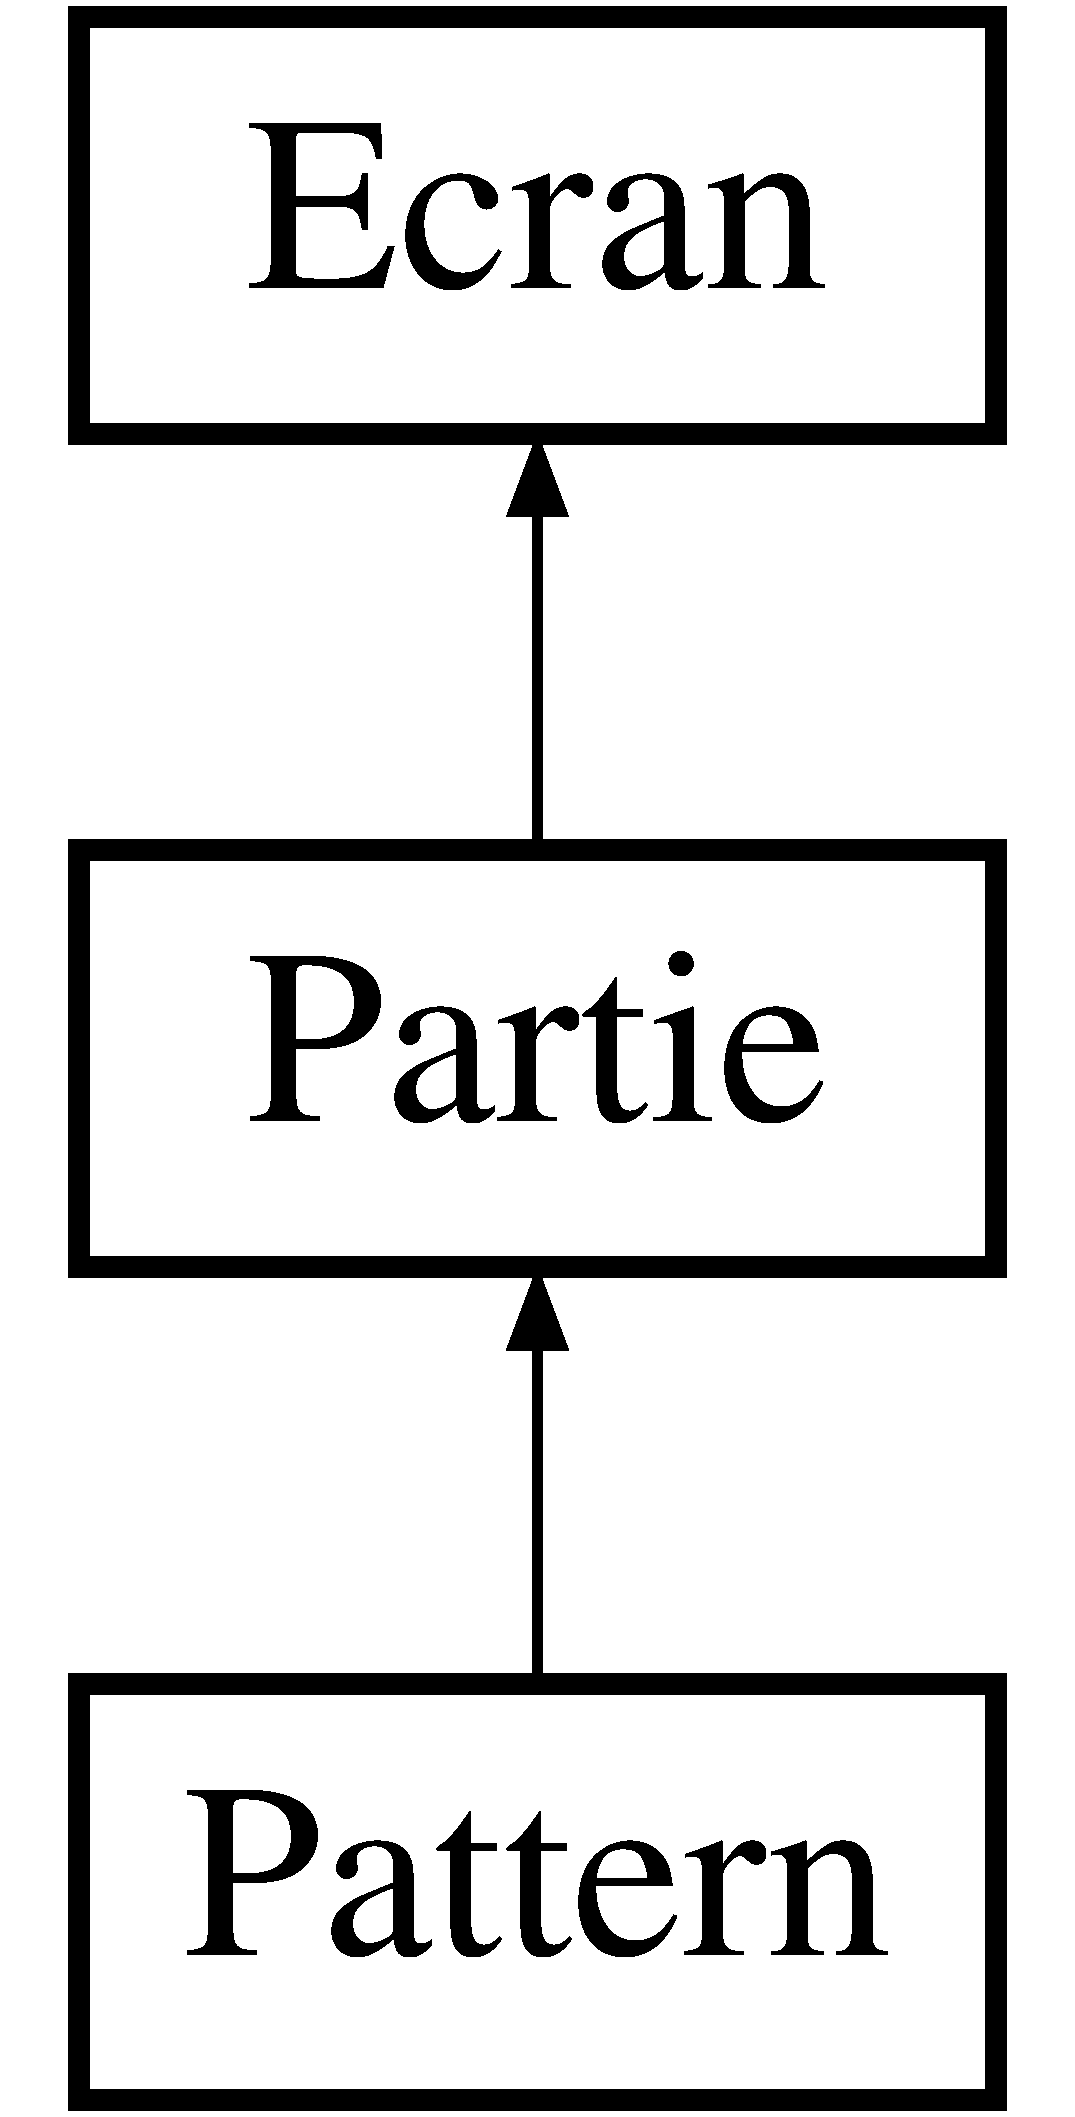
\includegraphics[height=3.000000cm]{class_pattern}
\end{center}
\end{figure}
\subsection*{Additional Inherited Members}


The documentation for this class was generated from the following file\+:\begin{DoxyCompactItemize}
\item 
src/\+Pattern/\mbox{\hyperlink{_pattern_8h}{Pattern.\+h}}\end{DoxyCompactItemize}

\hypertarget{class_proj_bismillah}{}\section{Référence de la classe Proj\+Bismillah}
\label{class_proj_bismillah}\index{Proj\+Bismillah@{Proj\+Bismillah}}


{\ttfamily \#include $<$Proj\+Bismillah.\+h$>$}



Graphe d\textquotesingle{}héritage de Proj\+Bismillah\+:
% FIG 0


Graphe de collaboration de Proj\+Bismillah\+:
% FIG 1
\subsection*{Fonctions membres publiques}
\begin{DoxyCompactItemize}
\item 
\hyperlink{class_proj_bismillah_a6a26d25b463a7ae0298abf31085ff7c3}{Proj\+Bismillah} (int x, int y, sf\+::\+Sound sound, \hyperlink{constantes_8h_a08fa5554288d5031a8f3bb83cc04ee83}{Equipe} equipe=\hyperlink{constantes_8h_a08fa5554288d5031a8f3bb83cc04ee83a31ad00d2974deb1103ea000de3bff57d}{N\+E\+U\+T\+RE})
\begin{DoxyCompactList}\small\item\em Constructeur. \end{DoxyCompactList}\item 
void \hyperlink{class_proj_bismillah_a6db489d8ffa3986d073518cf79416c98}{gestion} (sf\+::\+Render\+Window \&window, sf\+::\+Time temps\+Ecoule)
\item 
void \hyperlink{class_proj_bismillah_a23bdc7268920f71d218198ae26021a4f}{agit} (\hyperlink{class_entite}{Entite} \&e)
\begin{DoxyCompactList}\small\item\em Réalise l\textquotesingle{}action que l\textquotesingle{}{\ttfamily \hyperlink{class_entite}{Entite}} doit faire sur le vaisseau. \end{DoxyCompactList}\end{DoxyCompactItemize}
\subsection*{Membres hérités additionnels}


\subsection{Documentation des constructeurs et destructeur}
\mbox{\Hypertarget{class_proj_bismillah_a6a26d25b463a7ae0298abf31085ff7c3}\label{class_proj_bismillah_a6a26d25b463a7ae0298abf31085ff7c3}} 
\index{Proj\+Bismillah@{Proj\+Bismillah}!Proj\+Bismillah@{Proj\+Bismillah}}
\index{Proj\+Bismillah@{Proj\+Bismillah}!Proj\+Bismillah@{Proj\+Bismillah}}
\subsubsection{\texorpdfstring{Proj\+Bismillah()}{ProjBismillah()}}
{\footnotesize\ttfamily Proj\+Bismillah\+::\+Proj\+Bismillah (\begin{DoxyParamCaption}\item[{int}]{x,  }\item[{int}]{y,  }\item[{sf\+::\+Sound}]{sound,  }\item[{\hyperlink{constantes_8h_a08fa5554288d5031a8f3bb83cc04ee83}{Equipe}}]{equipe = {\ttfamily \hyperlink{constantes_8h_a08fa5554288d5031a8f3bb83cc04ee83a31ad00d2974deb1103ea000de3bff57d}{N\+E\+U\+T\+RE}} }\end{DoxyParamCaption})}



Constructeur. 


\begin{DoxyParams}{Paramètres}
{\em x} & Abscisse de la position de départ du projectile \\
\hline
{\em y} & Ordonnée de la position de départ du projectile \\
\hline
{\em sound} & Son par défaut donné par la capacité qui crée le proj \\
\hline
{\em equipe} & Représente l\textquotesingle{}équipe depuis \+\_\+constante.\+h \+: enum Equipe\\
\hline
\end{DoxyParams}
Créer un projectile piou à la position donnée en paramètre 

\subsection{Documentation des fonctions membres}
\mbox{\Hypertarget{class_proj_bismillah_a23bdc7268920f71d218198ae26021a4f}\label{class_proj_bismillah_a23bdc7268920f71d218198ae26021a4f}} 
\index{Proj\+Bismillah@{Proj\+Bismillah}!agit@{agit}}
\index{agit@{agit}!Proj\+Bismillah@{Proj\+Bismillah}}
\subsubsection{\texorpdfstring{agit()}{agit()}}
{\footnotesize\ttfamily void Proj\+Bismillah\+::agit (\begin{DoxyParamCaption}\item[{\hyperlink{class_entite}{Entite} \&}]{e }\end{DoxyParamCaption})\hspace{0.3cm}{\ttfamily [inline]}, {\ttfamily [virtual]}}



Réalise l\textquotesingle{}action que l\textquotesingle{}{\ttfamily \hyperlink{class_entite}{Entite}} doit faire sur le vaisseau. 

Fonction virtuelle qui doit être surchargée pour les classes héritées. Elle réalise l\textquotesingle{}action que l\textquotesingle{}{\ttfamily \hyperlink{class_entite}{Entite}} appelant sur l\textquotesingle{}{\ttfamily \hyperlink{class_entite}{Entite}} passé en paramètre (dégats, changement de stat, ...) 
\begin{DoxyParams}{Paramètres}
{\em e} & Une {\ttfamily \hyperlink{class_entite}{Entite}} sur lequel l\textquotesingle{}action de l\textquotesingle{}{\ttfamily \hyperlink{class_entite}{Entite}} va se faire \\
\hline
\end{DoxyParams}


Implémente \hyperlink{class_entite_a848ec47afac1d7ba970a2bcab5dc7b3b}{Entite}.

\mbox{\Hypertarget{class_proj_bismillah_a6db489d8ffa3986d073518cf79416c98}\label{class_proj_bismillah_a6db489d8ffa3986d073518cf79416c98}} 
\index{Proj\+Bismillah@{Proj\+Bismillah}!gestion@{gestion}}
\index{gestion@{gestion}!Proj\+Bismillah@{Proj\+Bismillah}}
\subsubsection{\texorpdfstring{gestion()}{gestion()}}
{\footnotesize\ttfamily void Proj\+Bismillah\+::gestion (\begin{DoxyParamCaption}\item[{sf\+::\+Render\+Window \&}]{window,  }\item[{sf\+::\+Time}]{temps\+Ecoule }\end{DoxyParamCaption})\hspace{0.3cm}{\ttfamily [inline]}, {\ttfamily [virtual]}}



Implémente \hyperlink{class_projectile_a09e02b793473660fc59a329a4dfea0ec}{Projectile}.



La documentation de cette classe a été générée à partir des fichiers suivants \+:\begin{DoxyCompactItemize}
\item 
src/\+Projectiles/\hyperlink{_proj_bismillah_8h}{Proj\+Bismillah.\+h}\item 
src/\+Projectiles/\hyperlink{_proj_bismillah_8cpp}{Proj\+Bismillah.\+cpp}\end{DoxyCompactItemize}

\hypertarget{class_proj_boing}{}\section{Proj\+Boing Class Reference}
\label{class_proj_boing}\index{Proj\+Boing@{Proj\+Boing}}


\mbox{\hyperlink{class_projectile}{Projectile}} de test.  




{\ttfamily \#include $<$Proj\+Boing.\+h$>$}

Inheritance diagram for Proj\+Boing\+:\begin{figure}[H]
\begin{center}
\leavevmode
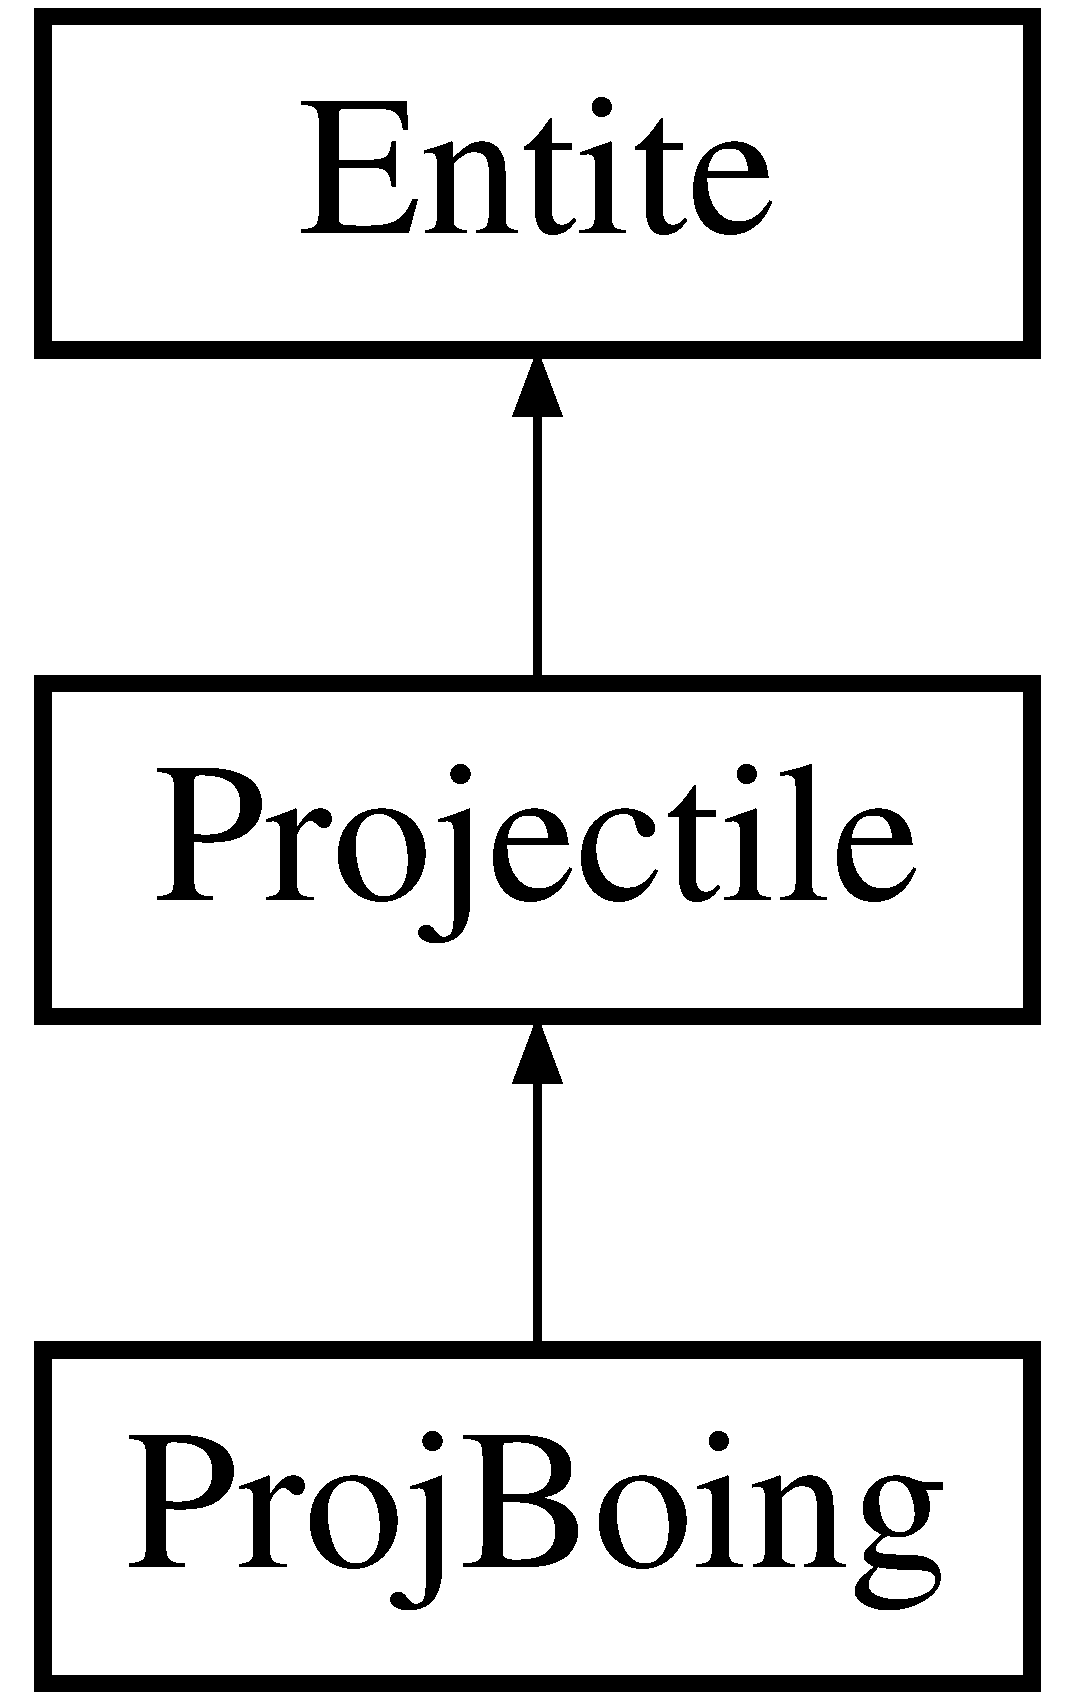
\includegraphics[height=3.000000cm]{class_proj_boing}
\end{center}
\end{figure}
\subsection*{Public Member Functions}
\begin{DoxyCompactItemize}
\item 
\mbox{\hyperlink{class_proj_boing_a4470a575e57978e4941b5771f710d7f3}{Proj\+Boing}} (\mbox{\hyperlink{class_ecran}{Ecran}} \&ecran, std\+::shared\+\_\+ptr$<$ \mbox{\hyperlink{class_entite}{Entite}} $>$ lanceur, std\+::vector$<$ sf\+::\+Sprite $>$ \&sprite, std\+::vector$<$ sf\+::\+Sound $>$ \&sound, \mbox{\hyperlink{constantes_8h_a08fa5554288d5031a8f3bb83cc04ee83}{Equipe}} equipe=\mbox{\hyperlink{constantes_8h_a08fa5554288d5031a8f3bb83cc04ee83a31ad00d2974deb1103ea000de3bff57d}{N\+E\+U\+T\+RE}})
\item 
\mbox{\hyperlink{class_proj_boing_a3b5745800aa7ce95337b6e89f06d2d43}{$\sim$\+Proj\+Boing}} ()
\begin{DoxyCompactList}\small\item\em Destructeur. \end{DoxyCompactList}\item 
void \mbox{\hyperlink{class_proj_boing_ac0d11abb68efb90dba3529d2bf1ce4f2}{gestion}} ()
\begin{DoxyCompactList}\small\item\em Gestion du projectile. \end{DoxyCompactList}\item 
void \mbox{\hyperlink{class_proj_boing_acbee1a0aa00582682ce755e1b19d687a}{agit}} (\mbox{\hyperlink{class_entite}{Entite}} \&proj)
\begin{DoxyCompactList}\small\item\em Procédure lorsque le projectile agit avec unvaisseau. \end{DoxyCompactList}\end{DoxyCompactItemize}
\subsection*{Additional Inherited Members}


\subsection{Detailed Description}
\mbox{\hyperlink{class_projectile}{Projectile}} de test. 

Lance 4 boules qui rebondissent sur les bord de l\textquotesingle{}écran 

\subsection{Constructor \& Destructor Documentation}
\mbox{\Hypertarget{class_proj_boing_a4470a575e57978e4941b5771f710d7f3}\label{class_proj_boing_a4470a575e57978e4941b5771f710d7f3}} 
\index{Proj\+Boing@{Proj\+Boing}!Proj\+Boing@{Proj\+Boing}}
\index{Proj\+Boing@{Proj\+Boing}!Proj\+Boing@{Proj\+Boing}}
\subsubsection{\texorpdfstring{Proj\+Boing()}{ProjBoing()}}
{\footnotesize\ttfamily Proj\+Boing\+::\+Proj\+Boing (\begin{DoxyParamCaption}\item[{\mbox{\hyperlink{class_ecran}{Ecran}} \&}]{ecran,  }\item[{std\+::shared\+\_\+ptr$<$ \mbox{\hyperlink{class_entite}{Entite}} $>$}]{lanceur,  }\item[{std\+::vector$<$ sf\+::\+Sprite $>$ \&}]{sprite,  }\item[{std\+::vector$<$ sf\+::\+Sound $>$ \&}]{sound,  }\item[{\mbox{\hyperlink{constantes_8h_a08fa5554288d5031a8f3bb83cc04ee83}{Equipe}}}]{equipe = {\ttfamily \mbox{\hyperlink{constantes_8h_a08fa5554288d5031a8f3bb83cc04ee83a31ad00d2974deb1103ea000de3bff57d}{N\+E\+U\+T\+RE}}} }\end{DoxyParamCaption})}

\mbox{\Hypertarget{class_proj_boing_a3b5745800aa7ce95337b6e89f06d2d43}\label{class_proj_boing_a3b5745800aa7ce95337b6e89f06d2d43}} 
\index{Proj\+Boing@{Proj\+Boing}!````~Proj\+Boing@{$\sim$\+Proj\+Boing}}
\index{````~Proj\+Boing@{$\sim$\+Proj\+Boing}!Proj\+Boing@{Proj\+Boing}}
\subsubsection{\texorpdfstring{$\sim$\+Proj\+Boing()}{~ProjBoing()}}
{\footnotesize\ttfamily Proj\+Boing\+::$\sim$\+Proj\+Boing (\begin{DoxyParamCaption}{ }\end{DoxyParamCaption})\hspace{0.3cm}{\ttfamily [inline]}}



Destructeur. 

Vide 

\subsection{Member Function Documentation}
\mbox{\Hypertarget{class_proj_boing_acbee1a0aa00582682ce755e1b19d687a}\label{class_proj_boing_acbee1a0aa00582682ce755e1b19d687a}} 
\index{Proj\+Boing@{Proj\+Boing}!agit@{agit}}
\index{agit@{agit}!Proj\+Boing@{Proj\+Boing}}
\subsubsection{\texorpdfstring{agit()}{agit()}}
{\footnotesize\ttfamily Proj\+Boing\+::agit (\begin{DoxyParamCaption}\item[{\mbox{\hyperlink{class_entite}{Entite}} \&}]{proj }\end{DoxyParamCaption})\hspace{0.3cm}{\ttfamily [virtual]}}



Procédure lorsque le projectile agit avec unvaisseau. 


\begin{DoxyParams}{Parameters}
{\em \mbox{\hyperlink{class_vaisseau}{Vaisseau}}} & à modifier\\
\hline
\end{DoxyParams}
Vide 

Implements \mbox{\hyperlink{class_entite_a848ec47afac1d7ba970a2bcab5dc7b3b}{Entite}}.

\mbox{\Hypertarget{class_proj_boing_ac0d11abb68efb90dba3529d2bf1ce4f2}\label{class_proj_boing_ac0d11abb68efb90dba3529d2bf1ce4f2}} 
\index{Proj\+Boing@{Proj\+Boing}!gestion@{gestion}}
\index{gestion@{gestion}!Proj\+Boing@{Proj\+Boing}}
\subsubsection{\texorpdfstring{gestion()}{gestion()}}
{\footnotesize\ttfamily Proj\+Boing\+::gestion (\begin{DoxyParamCaption}{ }\end{DoxyParamCaption})\hspace{0.3cm}{\ttfamily [virtual]}}



Gestion du projectile. 


\begin{DoxyParams}{Parameters}
{\em window} & Fenetre de jeu \\
\hline
{\em temps\+Ecoule} & Temps écoulé depuis le dernier appel\\
\hline
\end{DoxyParams}
Gestion du déplacement et de la collision avec les bords 

Implements \mbox{\hyperlink{class_projectile_ad8fae955389ff8944830e9d80e0f1ce1}{Projectile}}.



The documentation for this class was generated from the following files\+:\begin{DoxyCompactItemize}
\item 
src/\+Projectiles/\mbox{\hyperlink{_proj_boing_8h}{Proj\+Boing.\+h}}\item 
src/\+Projectiles/\mbox{\hyperlink{_proj_boing_8cpp}{Proj\+Boing.\+cpp}}\end{DoxyCompactItemize}

\hypertarget{class_proj_bouclier_rond}{}\section{Proj\+Bouclier\+Rond Class Reference}
\label{class_proj_bouclier_rond}\index{Proj\+Bouclier\+Rond@{Proj\+Bouclier\+Rond}}


{\ttfamily \#include $<$Proj\+Bouclier\+Rond.\+h$>$}

Inheritance diagram for Proj\+Bouclier\+Rond\+:\begin{figure}[H]
\begin{center}
\leavevmode
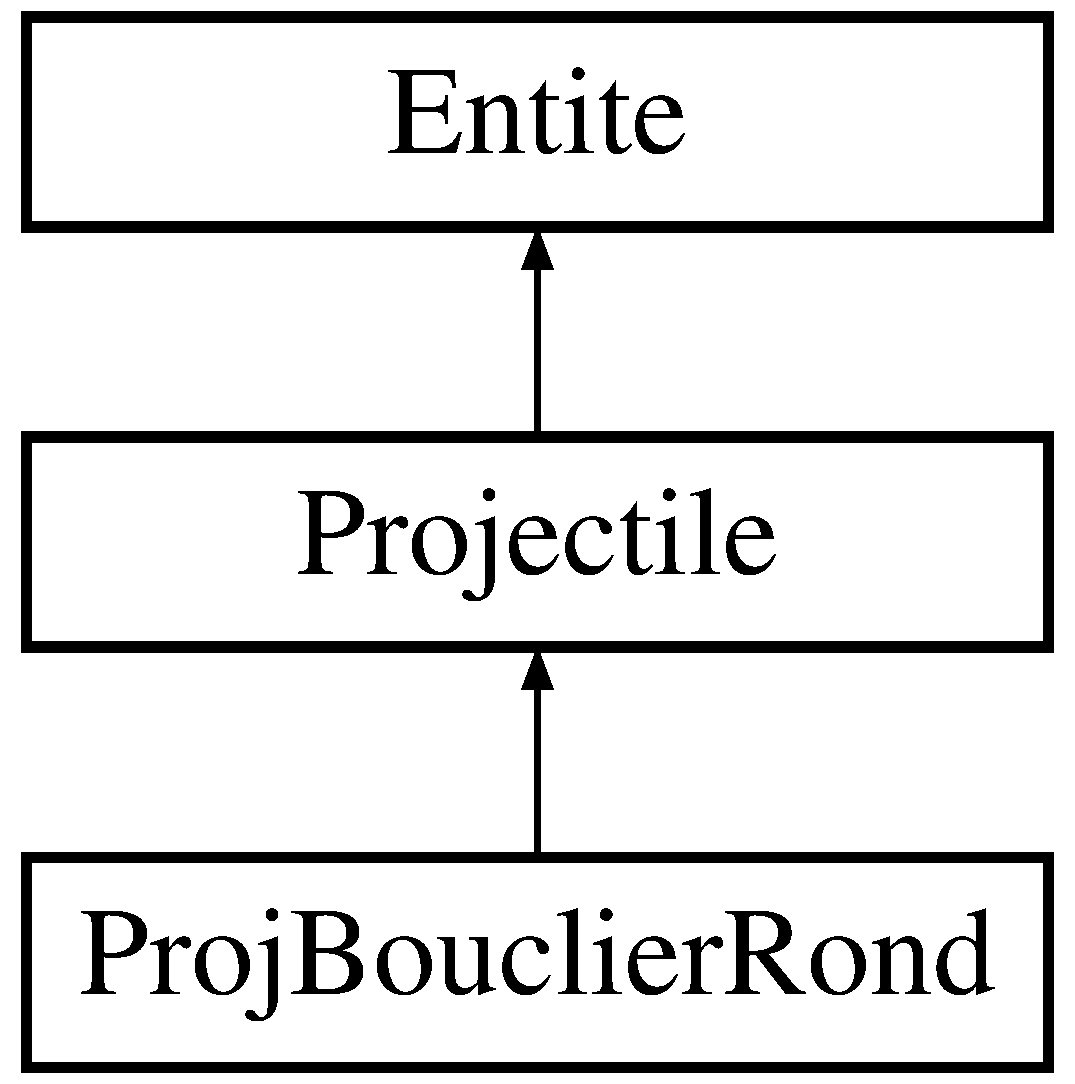
\includegraphics[height=3.000000cm]{class_proj_bouclier_rond}
\end{center}
\end{figure}
\subsection*{Public Member Functions}
\begin{DoxyCompactItemize}
\item 
\mbox{\hyperlink{class_proj_bouclier_rond_a4cbfae3e14164be2b345efaeac0b3abd}{$\sim$\+Proj\+Bouclier\+Rond}} () override
\item 
\mbox{\hyperlink{class_proj_bouclier_rond_ac0ace14849356b453582614a006116b5}{Proj\+Bouclier\+Rond}} (\mbox{\hyperlink{class_ecran}{Ecran}} \&ecran, std\+::shared\+\_\+ptr$<$ \mbox{\hyperlink{class_entite}{Entite}} $>$ lanceur, std\+::vector$<$ sf\+::\+Sprite $>$ \&sprite, std\+::vector$<$ sf\+::\+Sound $>$ \&sound, \mbox{\hyperlink{constantes_8h_a08fa5554288d5031a8f3bb83cc04ee83}{Equipe}} equipe)
\begin{DoxyCompactList}\small\item\em Constructeur. \end{DoxyCompactList}\item 
void \mbox{\hyperlink{class_proj_bouclier_rond_a13656b7dbcd9cac9a5df9baeab430103}{gestion}} ()
\begin{DoxyCompactList}\small\item\em Gestion du projectile. \end{DoxyCompactList}\item 
void \mbox{\hyperlink{class_proj_bouclier_rond_a60547ae68c6862f6e4c8b9cdd94bb52b}{agit}} (\mbox{\hyperlink{class_entite}{Entite}} \&e)
\begin{DoxyCompactList}\small\item\em Action lorsque collision avec une \mbox{\hyperlink{class_entite}{Entite}} collisionnable. \end{DoxyCompactList}\end{DoxyCompactItemize}
\subsection*{Additional Inherited Members}


\subsection{Constructor \& Destructor Documentation}
\mbox{\Hypertarget{class_proj_bouclier_rond_a4cbfae3e14164be2b345efaeac0b3abd}\label{class_proj_bouclier_rond_a4cbfae3e14164be2b345efaeac0b3abd}} 
\index{Proj\+Bouclier\+Rond@{Proj\+Bouclier\+Rond}!````~Proj\+Bouclier\+Rond@{$\sim$\+Proj\+Bouclier\+Rond}}
\index{````~Proj\+Bouclier\+Rond@{$\sim$\+Proj\+Bouclier\+Rond}!Proj\+Bouclier\+Rond@{Proj\+Bouclier\+Rond}}
\subsubsection{\texorpdfstring{$\sim$\+Proj\+Bouclier\+Rond()}{~ProjBouclierRond()}}
{\footnotesize\ttfamily Proj\+Bouclier\+Rond\+::$\sim$\+Proj\+Bouclier\+Rond (\begin{DoxyParamCaption}{ }\end{DoxyParamCaption})\hspace{0.3cm}{\ttfamily [inline]}, {\ttfamily [override]}}

\mbox{\Hypertarget{class_proj_bouclier_rond_ac0ace14849356b453582614a006116b5}\label{class_proj_bouclier_rond_ac0ace14849356b453582614a006116b5}} 
\index{Proj\+Bouclier\+Rond@{Proj\+Bouclier\+Rond}!Proj\+Bouclier\+Rond@{Proj\+Bouclier\+Rond}}
\index{Proj\+Bouclier\+Rond@{Proj\+Bouclier\+Rond}!Proj\+Bouclier\+Rond@{Proj\+Bouclier\+Rond}}
\subsubsection{\texorpdfstring{Proj\+Bouclier\+Rond()}{ProjBouclierRond()}}
{\footnotesize\ttfamily Proj\+Bouclier\+Rond\+::\+Proj\+Bouclier\+Rond (\begin{DoxyParamCaption}\item[{\mbox{\hyperlink{class_ecran}{Ecran}} \&}]{ecran,  }\item[{std\+::shared\+\_\+ptr$<$ \mbox{\hyperlink{class_entite}{Entite}} $>$}]{lanceur,  }\item[{std\+::vector$<$ sf\+::\+Sprite $>$ \&}]{sprite,  }\item[{std\+::vector$<$ sf\+::\+Sound $>$ \&}]{sound,  }\item[{\mbox{\hyperlink{constantes_8h_a08fa5554288d5031a8f3bb83cc04ee83}{Equipe}}}]{equipe }\end{DoxyParamCaption})}



Constructeur. 


\begin{DoxyParams}{Parameters}
{\em Entite\+\_\+liee} & entite sur laquelle s\textquotesingle{}applique le bouclier \\
\hline
{\em pvM} & pv max \\
\hline
{\em degats\+Coll} & dégats infligés lors d\textquotesingle{}une collision avec une \mbox{\hyperlink{class_entite}{Entite}} collisionnable Gestion du déplacement et de l\textquotesingle{}affichage \\
\hline
\end{DoxyParams}


\subsection{Member Function Documentation}
\mbox{\Hypertarget{class_proj_bouclier_rond_a60547ae68c6862f6e4c8b9cdd94bb52b}\label{class_proj_bouclier_rond_a60547ae68c6862f6e4c8b9cdd94bb52b}} 
\index{Proj\+Bouclier\+Rond@{Proj\+Bouclier\+Rond}!agit@{agit}}
\index{agit@{agit}!Proj\+Bouclier\+Rond@{Proj\+Bouclier\+Rond}}
\subsubsection{\texorpdfstring{agit()}{agit()}}
{\footnotesize\ttfamily Proj\+Bouclier\+Rond\+::agit (\begin{DoxyParamCaption}\item[{\mbox{\hyperlink{class_entite}{Entite}} \&}]{e }\end{DoxyParamCaption})\hspace{0.3cm}{\ttfamily [virtual]}}



Action lorsque collision avec une \mbox{\hyperlink{class_entite}{Entite}} collisionnable. 


\begin{DoxyParams}{Parameters}
{\em e} & \mbox{\hyperlink{class_entite}{Entite}}\\
\hline
\end{DoxyParams}
Inflige les dégat déterminés à la construction 

Implements \mbox{\hyperlink{class_entite_a848ec47afac1d7ba970a2bcab5dc7b3b}{Entite}}.

\mbox{\Hypertarget{class_proj_bouclier_rond_a13656b7dbcd9cac9a5df9baeab430103}\label{class_proj_bouclier_rond_a13656b7dbcd9cac9a5df9baeab430103}} 
\index{Proj\+Bouclier\+Rond@{Proj\+Bouclier\+Rond}!gestion@{gestion}}
\index{gestion@{gestion}!Proj\+Bouclier\+Rond@{Proj\+Bouclier\+Rond}}
\subsubsection{\texorpdfstring{gestion()}{gestion()}}
{\footnotesize\ttfamily Proj\+Bouclier\+Rond\+::gestion (\begin{DoxyParamCaption}{ }\end{DoxyParamCaption})\hspace{0.3cm}{\ttfamily [virtual]}}



Gestion du projectile. 


\begin{DoxyParams}{Parameters}
{\em window} & Fenetre de jeu\\
\hline
\end{DoxyParams}
Gestion du déplacement et de l\textquotesingle{}affichage \+: le bouclier reste lié à l\textquotesingle{}Entite\+\_\+liee 

Implements \mbox{\hyperlink{class_projectile_ad8fae955389ff8944830e9d80e0f1ce1}{Projectile}}.



The documentation for this class was generated from the following files\+:\begin{DoxyCompactItemize}
\item 
src/\+Projectiles/\mbox{\hyperlink{_proj_bouclier_rond_8h}{Proj\+Bouclier\+Rond.\+h}}\item 
src/\+Projectiles/\mbox{\hyperlink{_proj_bouclier_rond_8cpp}{Proj\+Bouclier\+Rond.\+cpp}}\end{DoxyCompactItemize}

\hypertarget{class_projectile}{}\section{Référence de la classe Projectile}
\label{class_projectile}\index{Projectile@{Projectile}}


Classe abstraite qui définit la structure générale d\textquotesingle{}un projectile, à faire hériter pour chaque projectile.  




{\ttfamily \#include $<$Projectile.\+h$>$}



Graphe d\textquotesingle{}héritage de Projectile\+:
\nopagebreak
\begin{figure}[H]
\begin{center}
\leavevmode
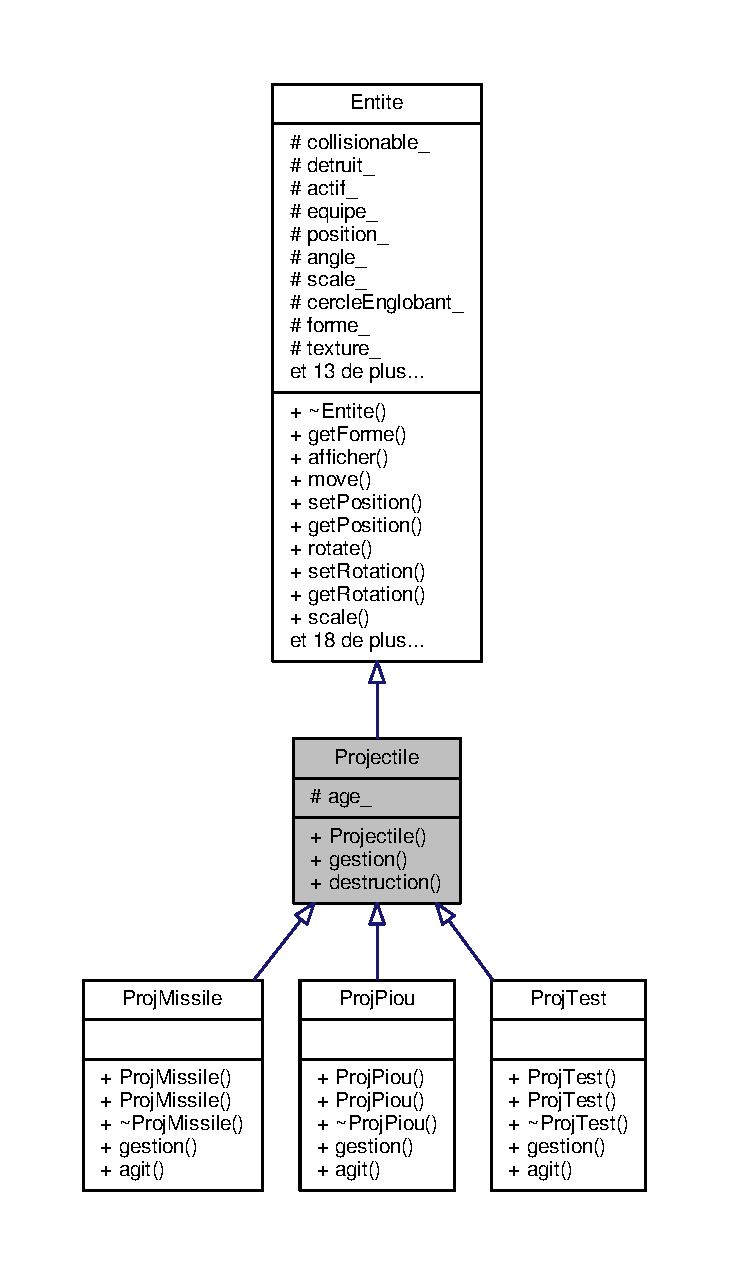
\includegraphics[width=204pt]{class_projectile__inherit__graph}
\end{center}
\end{figure}


Graphe de collaboration de Projectile\+:\nopagebreak
\begin{figure}[H]
\begin{center}
\leavevmode
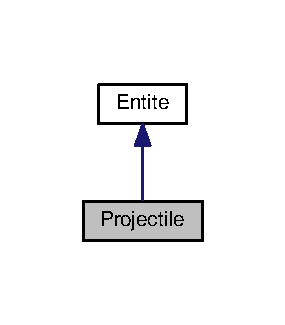
\includegraphics[width=137pt]{class_projectile__coll__graph}
\end{center}
\end{figure}
\subsection*{Fonctions membres publiques}
\begin{DoxyCompactItemize}
\item 
\hyperlink{class_projectile_ac536ed2aad56af866a2078b9a85aa16d}{Projectile} ()
\item 
virtual void \hyperlink{class_projectile_aa969857f9837d9be3a6ea415c9ba3ff1}{gestion} (sf\+::\+Render\+Window \&window)=0
\end{DoxyCompactItemize}
\subsection*{Attributs protégés}
\begin{DoxyCompactItemize}
\item 
int \hyperlink{class_projectile_a1f0a231e002d4796c32ccfeb36c887b1}{age\+\_\+}
\end{DoxyCompactItemize}


\subsection{Description détaillée}
Classe abstraite qui définit la structure générale d\textquotesingle{}un projectile, à faire hériter pour chaque projectile. 

Classe abstraite mère de chaque projectile en tant qu\textquotesingle{}entité propre. Une capacité peut créer plusieurs projectiles ; elle leur donne des méthodes qui les font exister dans la boucle de jeu \+: déplacement, test de collison, dégats... 

\subsection{Documentation des constructeurs et destructeur}
\mbox{\Hypertarget{class_projectile_ac536ed2aad56af866a2078b9a85aa16d}\label{class_projectile_ac536ed2aad56af866a2078b9a85aa16d}} 
\index{Projectile@{Projectile}!Projectile@{Projectile}}
\index{Projectile@{Projectile}!Projectile@{Projectile}}
\subsubsection{\texorpdfstring{Projectile()}{Projectile()}}
{\footnotesize\ttfamily Projectile\+::\+Projectile (\begin{DoxyParamCaption}{ }\end{DoxyParamCaption})}



\subsection{Documentation des fonctions membres}
\mbox{\Hypertarget{class_projectile_aa969857f9837d9be3a6ea415c9ba3ff1}\label{class_projectile_aa969857f9837d9be3a6ea415c9ba3ff1}} 
\index{Projectile@{Projectile}!gestion@{gestion}}
\index{gestion@{gestion}!Projectile@{Projectile}}
\subsubsection{\texorpdfstring{gestion()}{gestion()}}
{\footnotesize\ttfamily virtual void Projectile\+::gestion (\begin{DoxyParamCaption}\item[{sf\+::\+Render\+Window \&}]{window }\end{DoxyParamCaption})\hspace{0.3cm}{\ttfamily [pure virtual]}}



Implémenté dans \hyperlink{class_proj_test_af0b751a8e8cb0b7d10857722b691f3b6}{Proj\+Test}, et \hyperlink{class_proj_piou_a964182d333ed2bf64408a7812bc4cd28}{Proj\+Piou}.



\subsection{Documentation des données membres}
\mbox{\Hypertarget{class_projectile_a1f0a231e002d4796c32ccfeb36c887b1}\label{class_projectile_a1f0a231e002d4796c32ccfeb36c887b1}} 
\index{Projectile@{Projectile}!age\+\_\+@{age\+\_\+}}
\index{age\+\_\+@{age\+\_\+}!Projectile@{Projectile}}
\subsubsection{\texorpdfstring{age\+\_\+}{age\_}}
{\footnotesize\ttfamily int Projectile\+::age\+\_\+\hspace{0.3cm}{\ttfamily [protected]}}



La documentation de cette classe a été générée à partir des fichiers suivants \+:\begin{DoxyCompactItemize}
\item 
src/\+Projectiles/\hyperlink{_projectile_8h}{Projectile.\+h}\item 
src/\+Projectiles/\hyperlink{_projectile_8cpp}{Projectile.\+cpp}\end{DoxyCompactItemize}

\hypertarget{class_proj_missile}{}\section{Référence de la classe Proj\+Missile}
\label{class_proj_missile}\index{Proj\+Missile@{Proj\+Missile}}


{\ttfamily \#include $<$Proj\+Missile.\+h$>$}



Graphe d\textquotesingle{}héritage de Proj\+Missile\+:\nopagebreak
\begin{figure}[H]
\begin{center}
\leavevmode
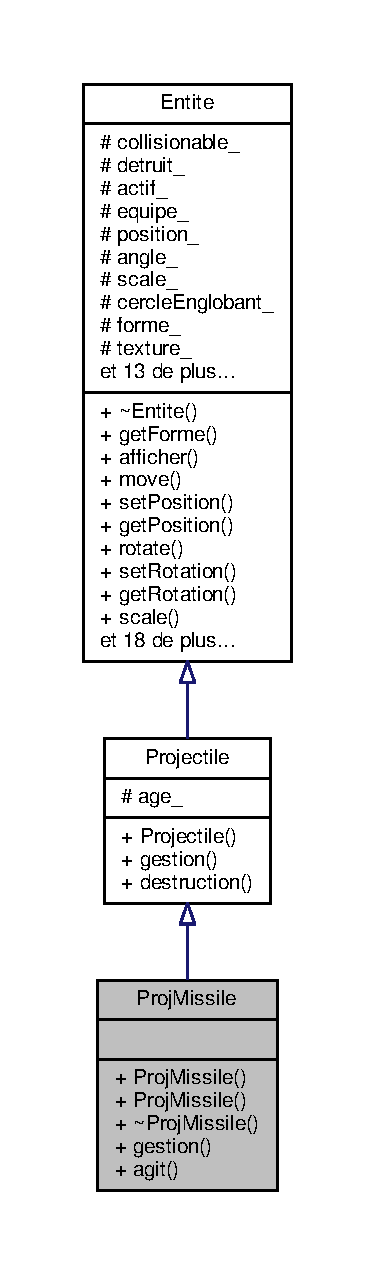
\includegraphics[height=550pt]{class_proj_missile__inherit__graph}
\end{center}
\end{figure}


Graphe de collaboration de Proj\+Missile\+:\nopagebreak
\begin{figure}[H]
\begin{center}
\leavevmode
\includegraphics[height=550pt]{class_proj_missile__coll__graph}
\end{center}
\end{figure}
\subsection*{Fonctions membres publiques}
\begin{DoxyCompactItemize}
\item 
\hyperlink{class_proj_missile_ab19da57422266894f8285b77ae1a2369}{Proj\+Missile} ()
\item 
\hyperlink{class_proj_missile_a1fedb310e8fc632c57c2b12ee4ee2a83}{Proj\+Missile} (float x, float y)
\item 
\hyperlink{class_proj_missile_adf1e62cc1a0c195b6de72ca7830338c5}{$\sim$\+Proj\+Missile} ()
\item 
void \hyperlink{class_proj_missile_a6e7a2c8180b7275a1d03340229d83bf3}{gestion} (sf\+::\+Render\+Window \&window, sf\+::\+Time temps\+Ecoule)
\begin{DoxyCompactList}\small\item\em Gestion du projectile. \end{DoxyCompactList}\item 
void \hyperlink{class_proj_missile_a8125c442857f7a0fc2d0ff442c39aca7}{agit} (\hyperlink{class_entite}{Entite} \&e)
\begin{DoxyCompactList}\small\item\em Proc�dure lorsque le projectile agit avec une \hyperlink{class_entite}{Entite}. \end{DoxyCompactList}\end{DoxyCompactItemize}
\subsection*{Membres hérités additionnels}


\subsection{Documentation des constructeurs et destructeur}
\mbox{\Hypertarget{class_proj_missile_ab19da57422266894f8285b77ae1a2369}\label{class_proj_missile_ab19da57422266894f8285b77ae1a2369}} 
\index{Proj\+Missile@{Proj\+Missile}!Proj\+Missile@{Proj\+Missile}}
\index{Proj\+Missile@{Proj\+Missile}!Proj\+Missile@{Proj\+Missile}}
\subsubsection{\texorpdfstring{Proj\+Missile()}{ProjMissile()}\hspace{0.1cm}{\footnotesize\ttfamily [1/2]}}
{\footnotesize\ttfamily Proj\+Missile\+::\+Proj\+Missile (\begin{DoxyParamCaption}{ }\end{DoxyParamCaption})}

\mbox{\Hypertarget{class_proj_missile_a1fedb310e8fc632c57c2b12ee4ee2a83}\label{class_proj_missile_a1fedb310e8fc632c57c2b12ee4ee2a83}} 
\index{Proj\+Missile@{Proj\+Missile}!Proj\+Missile@{Proj\+Missile}}
\index{Proj\+Missile@{Proj\+Missile}!Proj\+Missile@{Proj\+Missile}}
\subsubsection{\texorpdfstring{Proj\+Missile()}{ProjMissile()}\hspace{0.1cm}{\footnotesize\ttfamily [2/2]}}
{\footnotesize\ttfamily Proj\+Missile\+::\+Proj\+Missile (\begin{DoxyParamCaption}\item[{float}]{x,  }\item[{float}]{y }\end{DoxyParamCaption})}

\mbox{\Hypertarget{class_proj_missile_adf1e62cc1a0c195b6de72ca7830338c5}\label{class_proj_missile_adf1e62cc1a0c195b6de72ca7830338c5}} 
\index{Proj\+Missile@{Proj\+Missile}!````~Proj\+Missile@{$\sim$\+Proj\+Missile}}
\index{````~Proj\+Missile@{$\sim$\+Proj\+Missile}!Proj\+Missile@{Proj\+Missile}}
\subsubsection{\texorpdfstring{$\sim$\+Proj\+Missile()}{~ProjMissile()}}
{\footnotesize\ttfamily Proj\+Missile\+::$\sim$\+Proj\+Missile (\begin{DoxyParamCaption}{ }\end{DoxyParamCaption})}



\subsection{Documentation des fonctions membres}
\mbox{\Hypertarget{class_proj_missile_a8125c442857f7a0fc2d0ff442c39aca7}\label{class_proj_missile_a8125c442857f7a0fc2d0ff442c39aca7}} 
\index{Proj\+Missile@{Proj\+Missile}!agit@{agit}}
\index{agit@{agit}!Proj\+Missile@{Proj\+Missile}}
\subsubsection{\texorpdfstring{agit()}{agit()}}
{\footnotesize\ttfamily Proj\+Missile\+::agit (\begin{DoxyParamCaption}\item[{\hyperlink{class_entite}{Entite} \&}]{e }\end{DoxyParamCaption})\hspace{0.3cm}{\ttfamily [virtual]}}



Proc�dure lorsque le projectile agit avec une \hyperlink{class_entite}{Entite}. 


\begin{DoxyParams}{Paramètres}
{\em e} & \hyperlink{class_entite}{Entite} � modifier\\
\hline
\end{DoxyParams}
Vide 

Implémente \hyperlink{class_entite_a848ec47afac1d7ba970a2bcab5dc7b3b}{Entite}.

\mbox{\Hypertarget{class_proj_missile_a6e7a2c8180b7275a1d03340229d83bf3}\label{class_proj_missile_a6e7a2c8180b7275a1d03340229d83bf3}} 
\index{Proj\+Missile@{Proj\+Missile}!gestion@{gestion}}
\index{gestion@{gestion}!Proj\+Missile@{Proj\+Missile}}
\subsubsection{\texorpdfstring{gestion()}{gestion()}}
{\footnotesize\ttfamily Proj\+Missile\+::gestion (\begin{DoxyParamCaption}\item[{sf\+::\+Render\+Window \&}]{window,  }\item[{sf\+::\+Time}]{temps\+Ecoule }\end{DoxyParamCaption})\hspace{0.3cm}{\ttfamily [virtual]}}



Gestion du projectile. 


\begin{DoxyParams}{Paramètres}
{\em window} & Fenetre de jeu \\
\hline
{\em temps\+Ecoule} & Temps �coul� depuis le dernier appel\\
\hline
\end{DoxyParams}
Gestion du d�placement et de la collision avec les bords 

Implémente \hyperlink{class_projectile_a09e02b793473660fc59a329a4dfea0ec}{Projectile}.



La documentation de cette classe a été générée à partir des fichiers suivants \+:\begin{DoxyCompactItemize}
\item 
src/\+Projectiles/\hyperlink{_proj_missile_8h}{Proj\+Missile.\+h}\item 
src/\+Projectiles/\hyperlink{_proj_missile_8cpp}{Proj\+Missile.\+cpp}\end{DoxyCompactItemize}

\hypertarget{class_proj_piou}{}\section{Référence de la classe Proj\+Piou}
\label{class_proj_piou}\index{Proj\+Piou@{Proj\+Piou}}


{\ttfamily \#include $<$Proj\+Piou.\+h$>$}



Graphe d\textquotesingle{}héritage de Proj\+Piou\+:
\nopagebreak
\begin{figure}[H]
\begin{center}
\leavevmode
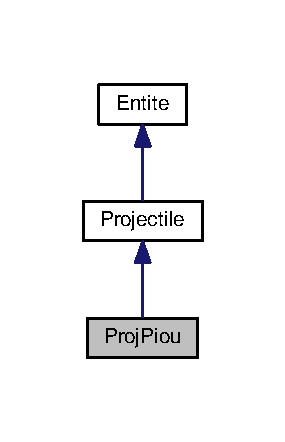
\includegraphics[width=137pt]{class_proj_piou__inherit__graph}
\end{center}
\end{figure}


Graphe de collaboration de Proj\+Piou\+:
\nopagebreak
\begin{figure}[H]
\begin{center}
\leavevmode
\includegraphics[width=137pt]{class_proj_piou__coll__graph}
\end{center}
\end{figure}
\subsection*{Fonctions membres publiques}
\begin{DoxyCompactItemize}
\item 
\hyperlink{class_proj_piou_a73d8a01dc3e09f926d14b95b673fd41d}{Proj\+Piou} ()
\item 
\hyperlink{class_proj_piou_a4aa12294ad8b563aa00848e395fdf06b}{Proj\+Piou} (int x, int y)
\item 
\hyperlink{class_proj_piou_a02224f153ad53afc2b1c40b986ec6492}{$\sim$\+Proj\+Piou} ()
\item 
void \hyperlink{class_proj_piou_a964182d333ed2bf64408a7812bc4cd28}{gestion} (sf\+::\+Render\+Window \&window)
\end{DoxyCompactItemize}
\subsection*{Membres hérités additionnels}


\subsection{Documentation des constructeurs et destructeur}
\mbox{\Hypertarget{class_proj_piou_a73d8a01dc3e09f926d14b95b673fd41d}\label{class_proj_piou_a73d8a01dc3e09f926d14b95b673fd41d}} 
\index{Proj\+Piou@{Proj\+Piou}!Proj\+Piou@{Proj\+Piou}}
\index{Proj\+Piou@{Proj\+Piou}!Proj\+Piou@{Proj\+Piou}}
\subsubsection{\texorpdfstring{Proj\+Piou()}{ProjPiou()}\hspace{0.1cm}{\footnotesize\ttfamily [1/2]}}
{\footnotesize\ttfamily Proj\+Piou\+::\+Proj\+Piou (\begin{DoxyParamCaption}{ }\end{DoxyParamCaption})}

\mbox{\Hypertarget{class_proj_piou_a4aa12294ad8b563aa00848e395fdf06b}\label{class_proj_piou_a4aa12294ad8b563aa00848e395fdf06b}} 
\index{Proj\+Piou@{Proj\+Piou}!Proj\+Piou@{Proj\+Piou}}
\index{Proj\+Piou@{Proj\+Piou}!Proj\+Piou@{Proj\+Piou}}
\subsubsection{\texorpdfstring{Proj\+Piou()}{ProjPiou()}\hspace{0.1cm}{\footnotesize\ttfamily [2/2]}}
{\footnotesize\ttfamily Proj\+Piou\+::\+Proj\+Piou (\begin{DoxyParamCaption}\item[{int}]{x,  }\item[{int}]{y }\end{DoxyParamCaption})}

\mbox{\Hypertarget{class_proj_piou_a02224f153ad53afc2b1c40b986ec6492}\label{class_proj_piou_a02224f153ad53afc2b1c40b986ec6492}} 
\index{Proj\+Piou@{Proj\+Piou}!````~Proj\+Piou@{$\sim$\+Proj\+Piou}}
\index{````~Proj\+Piou@{$\sim$\+Proj\+Piou}!Proj\+Piou@{Proj\+Piou}}
\subsubsection{\texorpdfstring{$\sim$\+Proj\+Piou()}{~ProjPiou()}}
{\footnotesize\ttfamily Proj\+Piou\+::$\sim$\+Proj\+Piou (\begin{DoxyParamCaption}{ }\end{DoxyParamCaption})}



\subsection{Documentation des fonctions membres}
\mbox{\Hypertarget{class_proj_piou_a964182d333ed2bf64408a7812bc4cd28}\label{class_proj_piou_a964182d333ed2bf64408a7812bc4cd28}} 
\index{Proj\+Piou@{Proj\+Piou}!gestion@{gestion}}
\index{gestion@{gestion}!Proj\+Piou@{Proj\+Piou}}
\subsubsection{\texorpdfstring{gestion()}{gestion()}}
{\footnotesize\ttfamily void Proj\+Piou\+::gestion (\begin{DoxyParamCaption}\item[{sf\+::\+Render\+Window \&}]{window }\end{DoxyParamCaption})\hspace{0.3cm}{\ttfamily [virtual]}}



Implémente \hyperlink{class_projectile_aa969857f9837d9be3a6ea415c9ba3ff1}{Projectile}.



La documentation de cette classe a été générée à partir des fichiers suivants \+:\begin{DoxyCompactItemize}
\item 
src/\+Projectiles/\hyperlink{_proj_piou_8h}{Proj\+Piou.\+h}\item 
src/\+Projectiles/\hyperlink{_proj_piou_8cpp}{Proj\+Piou.\+cpp}\end{DoxyCompactItemize}

\hypertarget{unionstd_1_1experimental_1_1storage__t}{}\section{std\+:\+:experimental\+:\+:storage\+\_\+t$<$ T $>$ Union Template Reference}
\label{unionstd_1_1experimental_1_1storage__t}\index{std\+::experimental\+::storage\+\_\+t$<$ T $>$@{std\+::experimental\+::storage\+\_\+t$<$ T $>$}}


{\ttfamily \#include $<$optional.\+h$>$}

\subsection*{Public Member Functions}
\begin{DoxyCompactItemize}
\item 
constexpr \mbox{\hyperlink{unionstd_1_1experimental_1_1storage__t_a66bf7a342f8770f3213d17b2a4b3b33c}{storage\+\_\+t}} (\mbox{\hyperlink{structstd_1_1experimental_1_1trivial__init__t}{trivial\+\_\+init\+\_\+t}}) noexcept
\item 
{\footnotesize template$<$class... Args$>$ }\\constexpr \mbox{\hyperlink{unionstd_1_1experimental_1_1storage__t_ae93191c4a215b166fe38fbafabd26449}{storage\+\_\+t}} (Args \&\&... args)
\item 
\mbox{\hyperlink{unionstd_1_1experimental_1_1storage__t_a9de04c8f12a996c2b9b55d430713b31e}{$\sim$storage\+\_\+t}} ()
\end{DoxyCompactItemize}
\subsection*{Public Attributes}
\begin{DoxyCompactItemize}
\item 
unsigned char \mbox{\hyperlink{unionstd_1_1experimental_1_1storage__t_a66c46e8a91805a1495127fa280a3f58a}{dummy\+\_\+}}
\item 
T \mbox{\hyperlink{unionstd_1_1experimental_1_1storage__t_afc411a630487df07bf6278ebbef1ebb7}{value\+\_\+}}
\end{DoxyCompactItemize}


\subsection{Constructor \& Destructor Documentation}
\mbox{\Hypertarget{unionstd_1_1experimental_1_1storage__t_a66bf7a342f8770f3213d17b2a4b3b33c}\label{unionstd_1_1experimental_1_1storage__t_a66bf7a342f8770f3213d17b2a4b3b33c}} 
\index{std\+::experimental\+::storage\+\_\+t@{std\+::experimental\+::storage\+\_\+t}!storage\+\_\+t@{storage\+\_\+t}}
\index{storage\+\_\+t@{storage\+\_\+t}!std\+::experimental\+::storage\+\_\+t@{std\+::experimental\+::storage\+\_\+t}}
\subsubsection{\texorpdfstring{storage\+\_\+t()}{storage\_t()}\hspace{0.1cm}{\footnotesize\ttfamily [1/2]}}
{\footnotesize\ttfamily template$<$class T$>$ \\
constexpr \mbox{\hyperlink{unionstd_1_1experimental_1_1storage__t}{std\+::experimental\+::storage\+\_\+t}}$<$ T $>$\+::\mbox{\hyperlink{unionstd_1_1experimental_1_1storage__t}{storage\+\_\+t}} (\begin{DoxyParamCaption}\item[{\mbox{\hyperlink{structstd_1_1experimental_1_1trivial__init__t}{trivial\+\_\+init\+\_\+t}}}]{ }\end{DoxyParamCaption})\hspace{0.3cm}{\ttfamily [inline]}, {\ttfamily [noexcept]}}

\mbox{\Hypertarget{unionstd_1_1experimental_1_1storage__t_ae93191c4a215b166fe38fbafabd26449}\label{unionstd_1_1experimental_1_1storage__t_ae93191c4a215b166fe38fbafabd26449}} 
\index{std\+::experimental\+::storage\+\_\+t@{std\+::experimental\+::storage\+\_\+t}!storage\+\_\+t@{storage\+\_\+t}}
\index{storage\+\_\+t@{storage\+\_\+t}!std\+::experimental\+::storage\+\_\+t@{std\+::experimental\+::storage\+\_\+t}}
\subsubsection{\texorpdfstring{storage\+\_\+t()}{storage\_t()}\hspace{0.1cm}{\footnotesize\ttfamily [2/2]}}
{\footnotesize\ttfamily template$<$class T$>$ \\
template$<$class... Args$>$ \\
constexpr \mbox{\hyperlink{unionstd_1_1experimental_1_1storage__t}{std\+::experimental\+::storage\+\_\+t}}$<$ T $>$\+::\mbox{\hyperlink{unionstd_1_1experimental_1_1storage__t}{storage\+\_\+t}} (\begin{DoxyParamCaption}\item[{Args \&\&...}]{args }\end{DoxyParamCaption})\hspace{0.3cm}{\ttfamily [inline]}}

\mbox{\Hypertarget{unionstd_1_1experimental_1_1storage__t_a9de04c8f12a996c2b9b55d430713b31e}\label{unionstd_1_1experimental_1_1storage__t_a9de04c8f12a996c2b9b55d430713b31e}} 
\index{std\+::experimental\+::storage\+\_\+t@{std\+::experimental\+::storage\+\_\+t}!````~storage\+\_\+t@{$\sim$storage\+\_\+t}}
\index{````~storage\+\_\+t@{$\sim$storage\+\_\+t}!std\+::experimental\+::storage\+\_\+t@{std\+::experimental\+::storage\+\_\+t}}
\subsubsection{\texorpdfstring{$\sim$storage\+\_\+t()}{~storage\_t()}}
{\footnotesize\ttfamily template$<$class T$>$ \\
\mbox{\hyperlink{unionstd_1_1experimental_1_1storage__t}{std\+::experimental\+::storage\+\_\+t}}$<$ T $>$\+::$\sim$\mbox{\hyperlink{unionstd_1_1experimental_1_1storage__t}{storage\+\_\+t}} (\begin{DoxyParamCaption}{ }\end{DoxyParamCaption})\hspace{0.3cm}{\ttfamily [inline]}}



\subsection{Member Data Documentation}
\mbox{\Hypertarget{unionstd_1_1experimental_1_1storage__t_a66c46e8a91805a1495127fa280a3f58a}\label{unionstd_1_1experimental_1_1storage__t_a66c46e8a91805a1495127fa280a3f58a}} 
\index{std\+::experimental\+::storage\+\_\+t@{std\+::experimental\+::storage\+\_\+t}!dummy\+\_\+@{dummy\+\_\+}}
\index{dummy\+\_\+@{dummy\+\_\+}!std\+::experimental\+::storage\+\_\+t@{std\+::experimental\+::storage\+\_\+t}}
\subsubsection{\texorpdfstring{dummy\+\_\+}{dummy\_}}
{\footnotesize\ttfamily template$<$class T$>$ \\
unsigned char \mbox{\hyperlink{unionstd_1_1experimental_1_1storage__t}{std\+::experimental\+::storage\+\_\+t}}$<$ T $>$\+::dummy\+\_\+}

\mbox{\Hypertarget{unionstd_1_1experimental_1_1storage__t_afc411a630487df07bf6278ebbef1ebb7}\label{unionstd_1_1experimental_1_1storage__t_afc411a630487df07bf6278ebbef1ebb7}} 
\index{std\+::experimental\+::storage\+\_\+t@{std\+::experimental\+::storage\+\_\+t}!value\+\_\+@{value\+\_\+}}
\index{value\+\_\+@{value\+\_\+}!std\+::experimental\+::storage\+\_\+t@{std\+::experimental\+::storage\+\_\+t}}
\subsubsection{\texorpdfstring{value\+\_\+}{value\_}}
{\footnotesize\ttfamily template$<$class T$>$ \\
T \mbox{\hyperlink{unionstd_1_1experimental_1_1storage__t}{std\+::experimental\+::storage\+\_\+t}}$<$ T $>$\+::value\+\_\+}



The documentation for this union was generated from the following file\+:\begin{DoxyCompactItemize}
\item 
src/\+Utilitaires/\mbox{\hyperlink{optional_8h}{optional.\+h}}\end{DoxyCompactItemize}

\hypertarget{structstd_1_1experimental_1_1trivial__init__t}{}\section{std\+:\+:experimental\+:\+:trivial\+\_\+init\+\_\+t Struct Reference}
\label{structstd_1_1experimental_1_1trivial__init__t}\index{std\+::experimental\+::trivial\+\_\+init\+\_\+t@{std\+::experimental\+::trivial\+\_\+init\+\_\+t}}


{\ttfamily \#include $<$optional.\+h$>$}



The documentation for this struct was generated from the following file\+:\begin{DoxyCompactItemize}
\item 
src/\+Utilitaires/\mbox{\hyperlink{optional_8h}{optional.\+h}}\end{DoxyCompactItemize}

\hypertarget{class_vague}{}\section{Référence de la classe Vague}
\label{class_vague}\index{Vague@{Vague}}


Classe qui décrit les vagues d\textquotesingle{}ennemis.  




{\ttfamily \#include $<$Vague.\+h$>$}



Graphe de collaboration de Vague\+:
% FIG 0
\subsection*{Fonctions membres publiques}
\begin{DoxyCompactItemize}
\item 
\hyperlink{class_vague_ab1e4786aa02ad641431b56658dbbaac3}{Vague} ()
\item 
\hyperlink{class_vague_a5a77009c7b36f68c5c5090c72294faa4}{Vague} (float t)
\item 
\hyperlink{class_vague_a72eb74bd6b6cc6de266fa4b8f77e56d4}{$\sim$\+Vague} ()
\item 
void \hyperlink{class_vague_a82124cdeb165825047f9dd8164e69a16}{ajouter\+Vaisseau} (float t, \hyperlink{class_vaisseau}{Vaisseau} $\ast$v)
\item 
void \hyperlink{class_vague_a37649d5f8063b1d516ce1f865a9d521d}{gestion} (std\+::vector$<$ \hyperlink{class_vaisseau}{Vaisseau} $\ast$$>$ \&vaisseaux, sf\+::\+Time t)
\begin{DoxyCompactList}\small\item\em Gere la vague. \end{DoxyCompactList}\item 
void \hyperlink{class_vague_a564d612f69751dd198ffa7ac61ea04dd}{set\+Temps\+Debut} (float t)
\begin{DoxyCompactList}\small\item\em Gere la vague. \end{DoxyCompactList}\item 
std\+::vector$<$ \hyperlink{struct_element_vague}{Element\+Vague} $>$ \hyperlink{class_vague_a1d927f38da46323e72208aaeb1b07d5b}{getv\+\_\+} ()
\item 
void \hyperlink{class_vague_aed7f0a70cc0d93ed686af4e100376974}{set\+Equipe\+All} (\hyperlink{constantes_8h_a08fa5554288d5031a8f3bb83cc04ee83}{Equipe} equipe)
\end{DoxyCompactItemize}


\subsection{Description détaillée}
Classe qui décrit les vagues d\textquotesingle{}ennemis. 

Cette classe pertmet de créer des vaisseaux selon un schéma défini, à partir d\textquotesingle{}un temps donné 

\subsection{Documentation des constructeurs et destructeur}
\mbox{\Hypertarget{class_vague_ab1e4786aa02ad641431b56658dbbaac3}\label{class_vague_ab1e4786aa02ad641431b56658dbbaac3}} 
\index{Vague@{Vague}!Vague@{Vague}}
\index{Vague@{Vague}!Vague@{Vague}}
\subsubsection{\texorpdfstring{Vague()}{Vague()}\hspace{0.1cm}{\footnotesize\ttfamily [1/2]}}
{\footnotesize\ttfamily Vague\+::\+Vague (\begin{DoxyParamCaption}{ }\end{DoxyParamCaption})}

\mbox{\Hypertarget{class_vague_a5a77009c7b36f68c5c5090c72294faa4}\label{class_vague_a5a77009c7b36f68c5c5090c72294faa4}} 
\index{Vague@{Vague}!Vague@{Vague}}
\index{Vague@{Vague}!Vague@{Vague}}
\subsubsection{\texorpdfstring{Vague()}{Vague()}\hspace{0.1cm}{\footnotesize\ttfamily [2/2]}}
{\footnotesize\ttfamily Vague\+::\+Vague (\begin{DoxyParamCaption}\item[{float}]{t }\end{DoxyParamCaption})\hspace{0.3cm}{\ttfamily [explicit]}}

\mbox{\Hypertarget{class_vague_a72eb74bd6b6cc6de266fa4b8f77e56d4}\label{class_vague_a72eb74bd6b6cc6de266fa4b8f77e56d4}} 
\index{Vague@{Vague}!````~Vague@{$\sim$\+Vague}}
\index{````~Vague@{$\sim$\+Vague}!Vague@{Vague}}
\subsubsection{\texorpdfstring{$\sim$\+Vague()}{~Vague()}}
{\footnotesize\ttfamily Vague\+::$\sim$\+Vague (\begin{DoxyParamCaption}{ }\end{DoxyParamCaption})}



\subsection{Documentation des fonctions membres}
\mbox{\Hypertarget{class_vague_a82124cdeb165825047f9dd8164e69a16}\label{class_vague_a82124cdeb165825047f9dd8164e69a16}} 
\index{Vague@{Vague}!ajouter\+Vaisseau@{ajouter\+Vaisseau}}
\index{ajouter\+Vaisseau@{ajouter\+Vaisseau}!Vague@{Vague}}
\subsubsection{\texorpdfstring{ajouter\+Vaisseau()}{ajouterVaisseau()}}
{\footnotesize\ttfamily void Vague\+::ajouter\+Vaisseau (\begin{DoxyParamCaption}\item[{float}]{t,  }\item[{\hyperlink{class_vaisseau}{Vaisseau} $\ast$}]{v }\end{DoxyParamCaption})}

\mbox{\Hypertarget{class_vague_a37649d5f8063b1d516ce1f865a9d521d}\label{class_vague_a37649d5f8063b1d516ce1f865a9d521d}} 
\index{Vague@{Vague}!gestion@{gestion}}
\index{gestion@{gestion}!Vague@{Vague}}
\subsubsection{\texorpdfstring{gestion()}{gestion()}}
{\footnotesize\ttfamily Vague\+::gestion (\begin{DoxyParamCaption}\item[{std\+::vector$<$ \hyperlink{class_vaisseau}{Vaisseau} $\ast$$>$ \&}]{vaisseaux,  }\item[{sf\+::\+Time}]{t }\end{DoxyParamCaption})}



Gere la vague. 


\begin{DoxyParams}{Paramètres}
{\em t} & Temps écoulé depuis le début de la boucle \\
\hline
{\em vaisseaux} & Vecteur de tous les vaisseaux présent à l\textquotesingle{}écran Gere le déclanchement de la vague et l\textquotesingle{}apparition des vaisseaux \\
\hline
\end{DoxyParams}
\mbox{\Hypertarget{class_vague_a1d927f38da46323e72208aaeb1b07d5b}\label{class_vague_a1d927f38da46323e72208aaeb1b07d5b}} 
\index{Vague@{Vague}!getv\+\_\+@{getv\+\_\+}}
\index{getv\+\_\+@{getv\+\_\+}!Vague@{Vague}}
\subsubsection{\texorpdfstring{getv\+\_\+()}{getv\_()}}
{\footnotesize\ttfamily std\+::vector$<$\hyperlink{struct_element_vague}{Element\+Vague}$>$ Vague\+::getv\+\_\+ (\begin{DoxyParamCaption}{ }\end{DoxyParamCaption})\hspace{0.3cm}{\ttfamily [inline]}}

\mbox{\Hypertarget{class_vague_aed7f0a70cc0d93ed686af4e100376974}\label{class_vague_aed7f0a70cc0d93ed686af4e100376974}} 
\index{Vague@{Vague}!set\+Equipe\+All@{set\+Equipe\+All}}
\index{set\+Equipe\+All@{set\+Equipe\+All}!Vague@{Vague}}
\subsubsection{\texorpdfstring{set\+Equipe\+All()}{setEquipeAll()}}
{\footnotesize\ttfamily void Vague\+::set\+Equipe\+All (\begin{DoxyParamCaption}\item[{\hyperlink{constantes_8h_a08fa5554288d5031a8f3bb83cc04ee83}{Equipe}}]{equipe }\end{DoxyParamCaption})\hspace{0.3cm}{\ttfamily [inline]}}

\mbox{\Hypertarget{class_vague_a564d612f69751dd198ffa7ac61ea04dd}\label{class_vague_a564d612f69751dd198ffa7ac61ea04dd}} 
\index{Vague@{Vague}!set\+Temps\+Debut@{set\+Temps\+Debut}}
\index{set\+Temps\+Debut@{set\+Temps\+Debut}!Vague@{Vague}}
\subsubsection{\texorpdfstring{set\+Temps\+Debut()}{setTempsDebut()}}
{\footnotesize\ttfamily Vague\+::set\+Temps\+Debut (\begin{DoxyParamCaption}\item[{float}]{t }\end{DoxyParamCaption})}



Gere la vague. 


\begin{DoxyParams}{Paramètres}
{\em t} & Temps de départ de la vague Fixe le temps de départ du début de la vague \\
\hline
\end{DoxyParams}


La documentation de cette classe a été générée à partir des fichiers suivants \+:\begin{DoxyCompactItemize}
\item 
src/\+Pattern/\hyperlink{_vague_8h}{Vague.\+h}\item 
src/\+Pattern/\hyperlink{_vague_8cpp}{Vague.\+cpp}\end{DoxyCompactItemize}

\hypertarget{class_vaisseau}{}\section{Référence de la classe Vaisseau}
\label{class_vaisseau}\index{Vaisseau@{Vaisseau}}


classe du vaisseau (véhicule) d\textquotesingle{}un joueur ou d\textquotesingle{}un ennemi  




{\ttfamily \#include $<$Vaisseau.\+h$>$}

\subsection*{Fonctions membres publiques}
\begin{DoxyCompactItemize}
\item 
\hyperlink{class_vaisseau_a7a6f829d62d9a0568c0c10d42c81bd47}{Vaisseau} (bool player)
\item 
\hyperlink{class_vaisseau_ae40b8e0143d6b736065207281bde2e8a}{$\sim$\+Vaisseau} ()
\end{DoxyCompactItemize}


\subsection{Description détaillée}
classe du vaisseau (véhicule) d\textquotesingle{}un joueur ou d\textquotesingle{}un ennemi 

Description détaillée 

\subsection{Documentation des constructeurs et destructeur}
\mbox{\Hypertarget{class_vaisseau_a7a6f829d62d9a0568c0c10d42c81bd47}\label{class_vaisseau_a7a6f829d62d9a0568c0c10d42c81bd47}} 
\index{Vaisseau@{Vaisseau}!Vaisseau@{Vaisseau}}
\index{Vaisseau@{Vaisseau}!Vaisseau@{Vaisseau}}
\subsubsection{\texorpdfstring{Vaisseau()}{Vaisseau()}}
{\footnotesize\ttfamily Vaisseau\+::\+Vaisseau (\begin{DoxyParamCaption}\item[{bool}]{player }\end{DoxyParamCaption})\hspace{0.3cm}{\ttfamily [explicit]}}

\mbox{\Hypertarget{class_vaisseau_ae40b8e0143d6b736065207281bde2e8a}\label{class_vaisseau_ae40b8e0143d6b736065207281bde2e8a}} 
\index{Vaisseau@{Vaisseau}!````~Vaisseau@{$\sim$\+Vaisseau}}
\index{````~Vaisseau@{$\sim$\+Vaisseau}!Vaisseau@{Vaisseau}}
\subsubsection{\texorpdfstring{$\sim$\+Vaisseau()}{~Vaisseau()}}
{\footnotesize\ttfamily Vaisseau\+::$\sim$\+Vaisseau (\begin{DoxyParamCaption}{ }\end{DoxyParamCaption})}



La documentation de cette classe a été générée à partir des fichiers suivants \+:\begin{DoxyCompactItemize}
\item 
src/\hyperlink{_vaisseau_8h}{Vaisseau.\+h}\item 
src/\hyperlink{_vaisseau_8cpp}{Vaisseau.\+cpp}\end{DoxyCompactItemize}

\hypertarget{class_vaisseau_attaquant}{}\section{Référence de la classe Vaisseau\+Attaquant}
\label{class_vaisseau_attaquant}\index{Vaisseau\+Attaquant@{Vaisseau\+Attaquant}}


classe d\textquotesingle{}un ennemi de base \+: l\textquotesingle{}attaquant  




{\ttfamily \#include $<$Vaisseau\+Attaquant.\+h$>$}



Graphe d\textquotesingle{}héritage de Vaisseau\+Attaquant\+:
% FIG 0


Graphe de collaboration de Vaisseau\+Attaquant\+:
% FIG 1
\subsection*{Fonctions membres publiques}
\begin{DoxyCompactItemize}
\item 
\hyperlink{class_vaisseau_attaquant_a58fd4ab933dd101db82b9287e0c0aafa}{Vaisseau\+Attaquant} (float x, float y, \hyperlink{_trajectoire_8h_afa7f6e8323d7ee755d93cd1f6019dd95}{Trajectoire} traj, float param1, float param2, float param3=0, float param4=0)
\item 
\hyperlink{class_vaisseau_attaquant_a2707dcc90692ba6132ec6aeb659d3620}{$\sim$\+Vaisseau\+Attaquant} ()
\item 
void \hyperlink{class_vaisseau_attaquant_ad95d76e5973affa6ef287edd7ad5310e}{gestion} (sf\+::\+Render\+Window \&window, sf\+::\+Time temps\+Ecoule, \hyperlink{_input_8h_a5588d60d674991c719a8df848313e966}{Input} \&input)
\begin{DoxyCompactList}\small\item\em Gère le comportement du vaisseau. \end{DoxyCompactList}\item 
void \hyperlink{class_vaisseau_attaquant_af804e1fd491301c2385e10d88f4892a6}{destruction} ()
\begin{DoxyCompactList}\small\item\em Procedure a effectuer lorsque le vaisseau est détruit. \end{DoxyCompactList}\end{DoxyCompactItemize}
\subsection*{Membres hérités additionnels}


\subsection{Description détaillée}
classe d\textquotesingle{}un ennemi de base \+: l\textquotesingle{}attaquant 

Attaquant \+: \hyperlink{class_vaisseau}{Vaisseau} ennemi Comportement \+: Déplacement (Linéaire, Parabolique, Sinsoidale) uniquement Tir de missile (\hyperlink{class_proj_missile}{Proj\+Missile}) 

\subsection{Documentation des constructeurs et destructeur}
\mbox{\Hypertarget{class_vaisseau_attaquant_a58fd4ab933dd101db82b9287e0c0aafa}\label{class_vaisseau_attaquant_a58fd4ab933dd101db82b9287e0c0aafa}} 
\index{Vaisseau\+Attaquant@{Vaisseau\+Attaquant}!Vaisseau\+Attaquant@{Vaisseau\+Attaquant}}
\index{Vaisseau\+Attaquant@{Vaisseau\+Attaquant}!Vaisseau\+Attaquant@{Vaisseau\+Attaquant}}
\subsubsection{\texorpdfstring{Vaisseau\+Attaquant()}{VaisseauAttaquant()}}
{\footnotesize\ttfamily Vaisseau\+Attaquant\+::\+Vaisseau\+Attaquant (\begin{DoxyParamCaption}\item[{float}]{x,  }\item[{float}]{y,  }\item[{\hyperlink{_trajectoire_8h_afa7f6e8323d7ee755d93cd1f6019dd95}{Trajectoire}}]{traj,  }\item[{float}]{param1,  }\item[{float}]{param2,  }\item[{float}]{param3 = {\ttfamily 0},  }\item[{float}]{param4 = {\ttfamily 0} }\end{DoxyParamCaption})}

\mbox{\Hypertarget{class_vaisseau_attaquant_a2707dcc90692ba6132ec6aeb659d3620}\label{class_vaisseau_attaquant_a2707dcc90692ba6132ec6aeb659d3620}} 
\index{Vaisseau\+Attaquant@{Vaisseau\+Attaquant}!````~Vaisseau\+Attaquant@{$\sim$\+Vaisseau\+Attaquant}}
\index{````~Vaisseau\+Attaquant@{$\sim$\+Vaisseau\+Attaquant}!Vaisseau\+Attaquant@{Vaisseau\+Attaquant}}
\subsubsection{\texorpdfstring{$\sim$\+Vaisseau\+Attaquant()}{~VaisseauAttaquant()}}
{\footnotesize\ttfamily Vaisseau\+Attaquant\+::$\sim$\+Vaisseau\+Attaquant (\begin{DoxyParamCaption}{ }\end{DoxyParamCaption})}



\subsection{Documentation des fonctions membres}
\mbox{\Hypertarget{class_vaisseau_attaquant_af804e1fd491301c2385e10d88f4892a6}\label{class_vaisseau_attaquant_af804e1fd491301c2385e10d88f4892a6}} 
\index{Vaisseau\+Attaquant@{Vaisseau\+Attaquant}!destruction@{destruction}}
\index{destruction@{destruction}!Vaisseau\+Attaquant@{Vaisseau\+Attaquant}}
\subsubsection{\texorpdfstring{destruction()}{destruction()}}
{\footnotesize\ttfamily Vaisseau\+Attaquant\+::destruction (\begin{DoxyParamCaption}{ }\end{DoxyParamCaption})\hspace{0.3cm}{\ttfamily [inline]}, {\ttfamily [virtual]}}



Procedure a effectuer lorsque le vaisseau est détruit. 

Détruit l\textquotesingle{}entité 

Implémente \hyperlink{class_vaisseau_af4f490c5fd9e171b23067ec73aa737ad}{Vaisseau}.

\mbox{\Hypertarget{class_vaisseau_attaquant_ad95d76e5973affa6ef287edd7ad5310e}\label{class_vaisseau_attaquant_ad95d76e5973affa6ef287edd7ad5310e}} 
\index{Vaisseau\+Attaquant@{Vaisseau\+Attaquant}!gestion@{gestion}}
\index{gestion@{gestion}!Vaisseau\+Attaquant@{Vaisseau\+Attaquant}}
\subsubsection{\texorpdfstring{gestion()}{gestion()}}
{\footnotesize\ttfamily Vaisseau\+Attaquant\+::gestion (\begin{DoxyParamCaption}\item[{sf\+::\+Render\+Window \&}]{window,  }\item[{sf\+::\+Time}]{temps\+Ecoule,  }\item[{\hyperlink{_input_8h_a5588d60d674991c719a8df848313e966}{Input} \&}]{input }\end{DoxyParamCaption})\hspace{0.3cm}{\ttfamily [virtual]}}



Gère le comportement du vaisseau. 


\begin{DoxyParams}{Paramètres}
{\em window} & Fenetre S\+F\+ML où le vaisseau sera affiché \\
\hline
{\em temps\+Ecoule} & Temps écoulé depuis le dernier appel \\
\hline
{\em input} & Classe Input donnant accés aux entrée\\
\hline
\end{DoxyParams}
Gère le déplacement et l\textquotesingle{}affichage du vaisseau 

Implémente \hyperlink{class_vaisseau_afaa179c1f03255d7869b8e2296ed8307}{Vaisseau}.



La documentation de cette classe a été générée à partir des fichiers suivants \+:\begin{DoxyCompactItemize}
\item 
src/\+Vaisseau/\hyperlink{_vaisseau_attaquant_8h}{Vaisseau\+Attaquant.\+h}\item 
src/\+Vaisseau/\hyperlink{_vaisseau_attaquant_8cpp}{Vaisseau\+Attaquant.\+cpp}\end{DoxyCompactItemize}

\hypertarget{class_vaisseau_bouclier}{}\section{Vaisseau\+Bouclier Class Reference}
\label{class_vaisseau_bouclier}\index{Vaisseau\+Bouclier@{Vaisseau\+Bouclier}}


classe d\textquotesingle{}un ennemi de base \+: le défenseur  




{\ttfamily \#include $<$Vaisseau\+Defenseur.\+h$>$}



\subsection{Detailed Description}
classe d\textquotesingle{}un ennemi de base \+: le défenseur 

Défenseur \+: \mbox{\hyperlink{class_vaisseau}{Vaisseau}} ennemi Comportement \+: Déplacement (Linéaire, Parabolique, Sinsoidale) Pas de Tir Possède un bouclier en face de lui destructible \+: \mbox{\hyperlink{class_vaiss_bouclier}{Vaiss\+Bouclier}} 

The documentation for this class was generated from the following file\+:\begin{DoxyCompactItemize}
\item 
src/\+Vaisseau/\mbox{\hyperlink{_vaisseau_defenseur_8h}{Vaisseau\+Defenseur.\+h}}\end{DoxyCompactItemize}

\hypertarget{class_vaisseau_defenseur}{}\section{Vaisseau\+Defenseur Class Reference}
\label{class_vaisseau_defenseur}\index{Vaisseau\+Defenseur@{Vaisseau\+Defenseur}}


{\ttfamily \#include $<$Vaisseau\+Defenseur.\+h$>$}

Inheritance diagram for Vaisseau\+Defenseur\+:\begin{figure}[H]
\begin{center}
\leavevmode
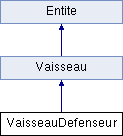
\includegraphics[height=3.000000cm]{class_vaisseau_defenseur}
\end{center}
\end{figure}
\subsection*{Public Member Functions}
\begin{DoxyCompactItemize}
\item 
\mbox{\hyperlink{class_vaisseau_defenseur_a19c543d8b04bdc0bb1d1c349bd3f1b99}{Vaisseau\+Defenseur}} (\mbox{\hyperlink{class_ecran}{Ecran}} \&ecran, float x, float y, \mbox{\hyperlink{def__type_8h_ad123ed7c93f42c8dd68e4af28b16b639}{vaisseau\+\_\+container}} \&vaisseaux, \mbox{\hyperlink{_trajectoire_8h_afa7f6e8323d7ee755d93cd1f6019dd95}{Trajectoire}} traj, float param1, float param2, float param3=0, float param4=0)
\begin{DoxyCompactList}\small\item\em Contructeur. \end{DoxyCompactList}\item 
\mbox{\hyperlink{class_vaisseau_defenseur_afb1098f176694c537f9a6c31da42d165}{$\sim$\+Vaisseau\+Defenseur}} ()
\begin{DoxyCompactList}\small\item\em Destructeur. \end{DoxyCompactList}\item 
void \mbox{\hyperlink{class_vaisseau_defenseur_a9d8301faaaebc09dd5e807e8ebe829ae}{gestion}} (\mbox{\hyperlink{def__type_8h_a87980cd8ee9533e561a73e8bbc728188}{proj\+\_\+container}} \&proj\+\_\+cont, \mbox{\hyperlink{_input_8h_a5588d60d674991c719a8df848313e966}{Input}} \&input) override
\begin{DoxyCompactList}\small\item\em Gère le comportement du vaisseau. \end{DoxyCompactList}\item 
void \mbox{\hyperlink{class_vaisseau_defenseur_aeaaaa161533c6aa07b627172d8657b3a}{destruction}} () override
\begin{DoxyCompactList}\small\item\em Procedure a effectuer lorsque le vaisseau est détruit. \end{DoxyCompactList}\end{DoxyCompactItemize}
\subsection*{Additional Inherited Members}


\subsection{Constructor \& Destructor Documentation}
\mbox{\Hypertarget{class_vaisseau_defenseur_a19c543d8b04bdc0bb1d1c349bd3f1b99}\label{class_vaisseau_defenseur_a19c543d8b04bdc0bb1d1c349bd3f1b99}} 
\index{Vaisseau\+Defenseur@{Vaisseau\+Defenseur}!Vaisseau\+Defenseur@{Vaisseau\+Defenseur}}
\index{Vaisseau\+Defenseur@{Vaisseau\+Defenseur}!Vaisseau\+Defenseur@{Vaisseau\+Defenseur}}
\subsubsection{\texorpdfstring{Vaisseau\+Defenseur()}{VaisseauDefenseur()}}
{\footnotesize\ttfamily Vaisseau\+Defenseur\+::\+Vaisseau\+Defenseur (\begin{DoxyParamCaption}\item[{\mbox{\hyperlink{class_ecran}{Ecran}} \&}]{ecran,  }\item[{float}]{x,  }\item[{float}]{y,  }\item[{\mbox{\hyperlink{def__type_8h_ad123ed7c93f42c8dd68e4af28b16b639}{vaisseau\+\_\+container}} \&}]{vaisseaux,  }\item[{\mbox{\hyperlink{_trajectoire_8h_afa7f6e8323d7ee755d93cd1f6019dd95}{Trajectoire}}}]{traj,  }\item[{float}]{param1,  }\item[{float}]{param2,  }\item[{float}]{param3 = {\ttfamily 0},  }\item[{float}]{param4 = {\ttfamily 0} }\end{DoxyParamCaption})}



Contructeur. 


\begin{DoxyParams}{Parameters}
{\em x} & Abscisse de la position de départ \\
\hline
{\em y} & Ordonnée de la position de départ \\
\hline
{\em vaisseaux} & Vecteur de tout les vaisseaux \\
\hline
{\em traj} & Trajectoire voulue (Linéaire, parabolique ou sinusoidale) \\
\hline
{\em param1} & Lineaire \+: Sens Parabolique \+: Sens Sinusoidale \+: Sens (1/-\/1) \\
\hline
{\em param2} & Lineaire \+: Pente Parabolique \+: Ordonnée de l\textquotesingle{}extremum Sinusoidale \+: Période (spatiale) \\
\hline
{\em param3} & Lineaire \+: Inutilisé Parabolique \+: Abscisse de l\textquotesingle{}extremum Sinusoidale \+: Amplitude \\
\hline
{\em param4} & Lineaire \+: Inutilisé Parabolique \+: Inutilisé Sinusoidale \+: Pente\\
\hline
\end{DoxyParams}
Initialise le vaisseau à position et à la trajectoires désirées Equations si le vaisseau est en fonction du temps écoulé depuis la création\+:
\begin{DoxyItemize}
\item Lineraire \+: x = x0 + sens$\ast$v$\ast$t y = pente$\ast$(x -\/ x0) + y0
\item Parabolique \+: x = x0 + sens$\ast$v$\ast$t (faux mais approximation si la parabole est assez large) y = (y0 -\/ ordonnee)/(x0 -\/ abscisse)$^\wedge$2 $\ast$ (x -\/ abscisse)$^\wedge$2 + ordonnee
\item Sinusoidale \+: x = x0 + sens$\ast$v$\ast$t (faux mais approximation si la différence de temps est très petite devant la période) y = pente $\ast$ (x -\/ x0) + y0 + amplitude $\ast$ sin(2$\ast$pi/période $\ast$ x) 
\end{DoxyItemize}\mbox{\Hypertarget{class_vaisseau_defenseur_afb1098f176694c537f9a6c31da42d165}\label{class_vaisseau_defenseur_afb1098f176694c537f9a6c31da42d165}} 
\index{Vaisseau\+Defenseur@{Vaisseau\+Defenseur}!````~Vaisseau\+Defenseur@{$\sim$\+Vaisseau\+Defenseur}}
\index{````~Vaisseau\+Defenseur@{$\sim$\+Vaisseau\+Defenseur}!Vaisseau\+Defenseur@{Vaisseau\+Defenseur}}
\subsubsection{\texorpdfstring{$\sim$\+Vaisseau\+Defenseur()}{~VaisseauDefenseur()}}
{\footnotesize\ttfamily Vaisseau\+Defenseur\+::$\sim$\+Vaisseau\+Defenseur (\begin{DoxyParamCaption}{ }\end{DoxyParamCaption})\hspace{0.3cm}{\ttfamily [inline]}}



Destructeur. 

Vide 

\subsection{Member Function Documentation}
\mbox{\Hypertarget{class_vaisseau_defenseur_aeaaaa161533c6aa07b627172d8657b3a}\label{class_vaisseau_defenseur_aeaaaa161533c6aa07b627172d8657b3a}} 
\index{Vaisseau\+Defenseur@{Vaisseau\+Defenseur}!destruction@{destruction}}
\index{destruction@{destruction}!Vaisseau\+Defenseur@{Vaisseau\+Defenseur}}
\subsubsection{\texorpdfstring{destruction()}{destruction()}}
{\footnotesize\ttfamily Vaisseau\+Defenseur\+::destruction (\begin{DoxyParamCaption}{ }\end{DoxyParamCaption})\hspace{0.3cm}{\ttfamily [override]}, {\ttfamily [virtual]}}



Procedure a effectuer lorsque le vaisseau est détruit. 

Détruit l\textquotesingle{}annexe bouclier 

Implements \mbox{\hyperlink{class_vaisseau_a6d7506acb12c0367989066c899ec7949}{Vaisseau}}.

\mbox{\Hypertarget{class_vaisseau_defenseur_a9d8301faaaebc09dd5e807e8ebe829ae}\label{class_vaisseau_defenseur_a9d8301faaaebc09dd5e807e8ebe829ae}} 
\index{Vaisseau\+Defenseur@{Vaisseau\+Defenseur}!gestion@{gestion}}
\index{gestion@{gestion}!Vaisseau\+Defenseur@{Vaisseau\+Defenseur}}
\subsubsection{\texorpdfstring{gestion()}{gestion()}}
{\footnotesize\ttfamily Vaisseau\+Defenseur\+::gestion (\begin{DoxyParamCaption}\item[{\mbox{\hyperlink{def__type_8h_a87980cd8ee9533e561a73e8bbc728188}{proj\+\_\+container}} \&}]{proj\+\_\+cont,  }\item[{\mbox{\hyperlink{_input_8h_a5588d60d674991c719a8df848313e966}{Input}} \&}]{input }\end{DoxyParamCaption})\hspace{0.3cm}{\ttfamily [override]}, {\ttfamily [virtual]}}



Gère le comportement du vaisseau. 


\begin{DoxyParams}{Parameters}
{\em window} & Fenetre S\+F\+ML où le vaisseau sera affiché \\
\hline
{\em temps\+Ecoule} & Temps écoulé depuis le dernier appel \\
\hline
{\em input} & Classe Input donnant accés aux entrée\\
\hline
\end{DoxyParams}
Gère le déplacement et l\textquotesingle{}affichage du vaisseau 

Implements \mbox{\hyperlink{class_vaisseau_aece43c3acf0e125226a03209f66c5eb4}{Vaisseau}}.



The documentation for this class was generated from the following files\+:\begin{DoxyCompactItemize}
\item 
src/\+Vaisseau/\mbox{\hyperlink{_vaisseau_defenseur_8h}{Vaisseau\+Defenseur.\+h}}\item 
src/\+Vaisseau/\mbox{\hyperlink{_vaisseau_defenseur_8cpp}{Vaisseau\+Defenseur.\+cpp}}\end{DoxyCompactItemize}

\hypertarget{class_vaisseau_defenseur_b}{}\section{Référence de la classe Vaisseau\+DefenseurB}
\label{class_vaisseau_defenseur_b}\index{Vaisseau\+DefenseurB@{Vaisseau\+DefenseurB}}


classe du bouclier du \hyperlink{class_vaisseau_defenseur}{Vaisseau\+Defenseur}  




{\ttfamily \#include $<$Vaisseau\+Defenseur\+B.\+h$>$}



Graphe d\textquotesingle{}héritage de Vaisseau\+DefenseurB\+:
% FIG 0


Graphe de collaboration de Vaisseau\+DefenseurB\+:
% FIG 1
\subsection*{Fonctions membres publiques}
\begin{DoxyCompactItemize}
\item 
\hyperlink{class_vaisseau_defenseur_b_a7f6ddaa53d153a14a760bc51945ebb30}{Vaisseau\+DefenseurB} (int nb, float x, float y, \hyperlink{class_vaisseau}{Vaisseau} $\ast$createur)
\begin{DoxyCompactList}\small\item\em Contructeur. \end{DoxyCompactList}\item 
\hyperlink{class_vaisseau_defenseur_b_acb6347ed84b0364d36bf581d7a3e1129}{$\sim$\+Vaisseau\+DefenseurB} ()
\item 
void \hyperlink{class_vaisseau_defenseur_b_aae8e2488b91dbd1ceef8969debbc234f}{gestion} (sf\+::\+Render\+Window \&window, sf\+::\+Time temps\+Ecoule, \hyperlink{_input_8h_a5588d60d674991c719a8df848313e966}{Input} \&input)
\begin{DoxyCompactList}\small\item\em Gère le comportement du vaisseau. \end{DoxyCompactList}\item 
void \hyperlink{class_vaisseau_defenseur_b_aba88319dcc7540dce39c164fa9853732}{destruction} ()
\begin{DoxyCompactList}\small\item\em Procedure a effectuer lorsque le vaisseau est détruit. \end{DoxyCompactList}\end{DoxyCompactItemize}
\subsection*{Membres hérités additionnels}


\subsection{Description détaillée}
classe du bouclier du \hyperlink{class_vaisseau_defenseur}{Vaisseau\+Defenseur} 

Bouclier \+: Module d\textquotesingle{}un vaisseau ennemi Comportement \+: Pas de déplacement Pas de tir 

\subsection{Documentation des constructeurs et destructeur}
\mbox{\Hypertarget{class_vaisseau_defenseur_b_a7f6ddaa53d153a14a760bc51945ebb30}\label{class_vaisseau_defenseur_b_a7f6ddaa53d153a14a760bc51945ebb30}} 
\index{Vaisseau\+DefenseurB@{Vaisseau\+DefenseurB}!Vaisseau\+DefenseurB@{Vaisseau\+DefenseurB}}
\index{Vaisseau\+DefenseurB@{Vaisseau\+DefenseurB}!Vaisseau\+DefenseurB@{Vaisseau\+DefenseurB}}
\subsubsection{\texorpdfstring{Vaisseau\+Defenseur\+B()}{VaisseauDefenseurB()}}
{\footnotesize\ttfamily Vaisseau\+Defenseur\+B\+::\+Vaisseau\+DefenseurB (\begin{DoxyParamCaption}\item[{int}]{nb,  }\item[{float}]{x,  }\item[{float}]{y,  }\item[{\hyperlink{class_vaisseau}{Vaisseau} $\ast$}]{createur }\end{DoxyParamCaption})}



Contructeur. 


\begin{DoxyParams}{Paramètres}
{\em x} & Abscisse de la position de départ \\
\hline
{\em y} & Ordonnée de la position de départ \\
\hline
{\em createur} & Createur du module Initialise le vaisseau à position et à la trajectoires désirées \\
\hline
\end{DoxyParams}
\mbox{\Hypertarget{class_vaisseau_defenseur_b_acb6347ed84b0364d36bf581d7a3e1129}\label{class_vaisseau_defenseur_b_acb6347ed84b0364d36bf581d7a3e1129}} 
\index{Vaisseau\+DefenseurB@{Vaisseau\+DefenseurB}!````~Vaisseau\+DefenseurB@{$\sim$\+Vaisseau\+DefenseurB}}
\index{````~Vaisseau\+DefenseurB@{$\sim$\+Vaisseau\+DefenseurB}!Vaisseau\+DefenseurB@{Vaisseau\+DefenseurB}}
\subsubsection{\texorpdfstring{$\sim$\+Vaisseau\+Defenseur\+B()}{~VaisseauDefenseurB()}}
{\footnotesize\ttfamily Vaisseau\+Defenseur\+B\+::$\sim$\+Vaisseau\+DefenseurB (\begin{DoxyParamCaption}{ }\end{DoxyParamCaption})}



\subsection{Documentation des fonctions membres}
\mbox{\Hypertarget{class_vaisseau_defenseur_b_aba88319dcc7540dce39c164fa9853732}\label{class_vaisseau_defenseur_b_aba88319dcc7540dce39c164fa9853732}} 
\index{Vaisseau\+DefenseurB@{Vaisseau\+DefenseurB}!destruction@{destruction}}
\index{destruction@{destruction}!Vaisseau\+DefenseurB@{Vaisseau\+DefenseurB}}
\subsubsection{\texorpdfstring{destruction()}{destruction()}}
{\footnotesize\ttfamily Vaisseau\+Defenseur\+B\+::destruction (\begin{DoxyParamCaption}{ }\end{DoxyParamCaption})\hspace{0.3cm}{\ttfamily [virtual]}}



Procedure a effectuer lorsque le vaisseau est détruit. 

Indique au créateur que l\textquotesingle{}annexe est détuite 

Implémente \hyperlink{class_vaisseau_af4f490c5fd9e171b23067ec73aa737ad}{Vaisseau}.

\mbox{\Hypertarget{class_vaisseau_defenseur_b_aae8e2488b91dbd1ceef8969debbc234f}\label{class_vaisseau_defenseur_b_aae8e2488b91dbd1ceef8969debbc234f}} 
\index{Vaisseau\+DefenseurB@{Vaisseau\+DefenseurB}!gestion@{gestion}}
\index{gestion@{gestion}!Vaisseau\+DefenseurB@{Vaisseau\+DefenseurB}}
\subsubsection{\texorpdfstring{gestion()}{gestion()}}
{\footnotesize\ttfamily Vaisseau\+Defenseur\+B\+::gestion (\begin{DoxyParamCaption}\item[{sf\+::\+Render\+Window \&}]{window,  }\item[{sf\+::\+Time}]{temps\+Ecoule,  }\item[{\hyperlink{_input_8h_a5588d60d674991c719a8df848313e966}{Input} \&}]{input }\end{DoxyParamCaption})\hspace{0.3cm}{\ttfamily [virtual]}}



Gère le comportement du vaisseau. 


\begin{DoxyParams}{Paramètres}
{\em window} & Fenetre S\+F\+ML où le vaisseau sera affiché \\
\hline
{\em temps\+Ecoule} & Temps écoulé depuis le dernier appel \\
\hline
{\em input} & Classe Input donnant accés aux entrée\\
\hline
\end{DoxyParams}
Gère le déplacement et l\textquotesingle{}affichage du vaisseau 

Implémente \hyperlink{class_vaisseau_afaa179c1f03255d7869b8e2296ed8307}{Vaisseau}.



La documentation de cette classe a été générée à partir des fichiers suivants \+:\begin{DoxyCompactItemize}
\item 
src/\+Vaisseau/\hyperlink{_vaisseau_defenseur_b_8h}{Vaisseau\+Defenseur\+B.\+h}\item 
src/\+Vaisseau/\hyperlink{_vaisseau_defenseur_b_8cpp}{Vaisseau\+Defenseur\+B.\+cpp}\end{DoxyCompactItemize}

\hypertarget{class_vaisseau_eclaireur}{}\section{Vaisseau\+Eclaireur Class Reference}
\label{class_vaisseau_eclaireur}\index{Vaisseau\+Eclaireur@{Vaisseau\+Eclaireur}}


classe d\textquotesingle{}un ennemi de base \+: l\textquotesingle{}éclaireur  




{\ttfamily \#include $<$Vaisseau\+Eclaireur.\+h$>$}

Inheritance diagram for Vaisseau\+Eclaireur\+:\begin{figure}[H]
\begin{center}
\leavevmode
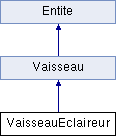
\includegraphics[height=3.000000cm]{class_vaisseau_eclaireur}
\end{center}
\end{figure}
\subsection*{Public Member Functions}
\begin{DoxyCompactItemize}
\item 
\mbox{\hyperlink{class_vaisseau_eclaireur_a3e02d4ef7316d0a44148c785c376deb2}{Vaisseau\+Eclaireur}} (\mbox{\hyperlink{class_ecran}{Ecran}} \&ecran, float x, float y, \mbox{\hyperlink{_trajectoire_8h_afa7f6e8323d7ee755d93cd1f6019dd95}{Trajectoire}} traj, double param1, double param2, double param3=0, double param4=0)
\begin{DoxyCompactList}\small\item\em Contructeur. \end{DoxyCompactList}\item 
\mbox{\hyperlink{class_vaisseau_eclaireur_a3e7ef82ff40bf4736d4285311dd8624c}{$\sim$\+Vaisseau\+Eclaireur}} ()
\begin{DoxyCompactList}\small\item\em Destructeurvide. \end{DoxyCompactList}\item 
void \mbox{\hyperlink{class_vaisseau_eclaireur_a66811ba07fd951304cca1c8be457b8e4}{gestion}} (\mbox{\hyperlink{def__type_8h_a87980cd8ee9533e561a73e8bbc728188}{proj\+\_\+container}} \&proj\+\_\+cont, \mbox{\hyperlink{_input_8h_a5588d60d674991c719a8df848313e966}{Input}} \&input) override
\begin{DoxyCompactList}\small\item\em Gère le comportement du vaisseau. \end{DoxyCompactList}\item 
void \mbox{\hyperlink{class_vaisseau_eclaireur_ab4ea82a8fc92dc27c6072481099518bc}{destruction}} () override
\begin{DoxyCompactList}\small\item\em Procedure a effectuer lorsque le vaisseau est détruit. \end{DoxyCompactList}\end{DoxyCompactItemize}
\subsection*{Additional Inherited Members}


\subsection{Detailed Description}
classe d\textquotesingle{}un ennemi de base \+: l\textquotesingle{}éclaireur 

Eclaireur \+: \mbox{\hyperlink{class_vaisseau}{Vaisseau}} ennemi Comportement \+: Déplacement (Linéaire, Parabolique, Sinsoidale) uniquement \+: pas de tir 

\subsection{Constructor \& Destructor Documentation}
\mbox{\Hypertarget{class_vaisseau_eclaireur_a3e02d4ef7316d0a44148c785c376deb2}\label{class_vaisseau_eclaireur_a3e02d4ef7316d0a44148c785c376deb2}} 
\index{Vaisseau\+Eclaireur@{Vaisseau\+Eclaireur}!Vaisseau\+Eclaireur@{Vaisseau\+Eclaireur}}
\index{Vaisseau\+Eclaireur@{Vaisseau\+Eclaireur}!Vaisseau\+Eclaireur@{Vaisseau\+Eclaireur}}
\subsubsection{\texorpdfstring{Vaisseau\+Eclaireur()}{VaisseauEclaireur()}}
{\footnotesize\ttfamily Vaisseau\+Eclaireur\+::\+Vaisseau\+Eclaireur (\begin{DoxyParamCaption}\item[{\mbox{\hyperlink{class_ecran}{Ecran}} \&}]{ecran,  }\item[{float}]{x,  }\item[{float}]{y,  }\item[{\mbox{\hyperlink{_trajectoire_8h_afa7f6e8323d7ee755d93cd1f6019dd95}{Trajectoire}}}]{traj,  }\item[{double}]{param1,  }\item[{double}]{param2,  }\item[{double}]{param3 = {\ttfamily 0},  }\item[{double}]{param4 = {\ttfamily 0} }\end{DoxyParamCaption})}



Contructeur. 


\begin{DoxyParams}{Parameters}
{\em x} & Abscisse de la position de départ \\
\hline
{\em y} & Ordonnée de la position de départ \\
\hline
{\em traj} & Trajectoire voulue (Linéaire, parabolique ou sinusoidale) \\
\hline
{\em param1} & Lineaire \+: Sens Parabolique \+: Sens Sinusoidale \+: Sens (1/-\/1) \\
\hline
{\em param2} & Lineaire \+: Pente Parabolique \+: Ordonnée de l\textquotesingle{}extremum Sinusoidale \+: Période (spatiale) \\
\hline
{\em param3} & Lineaire \+: Inutilisé Parabolique \+: Abscisse de l\textquotesingle{}extremum Sinusoidale \+: Amplitude \\
\hline
{\em param4} & Lineaire \+: Inutilisé Parabolique \+: Inutilisé Sinusoidale \+: Pente\\
\hline
\end{DoxyParams}
Initialise le vaisseau à position et à la trajectoires désirées Equations si le vaisseau est en fonction du temps écoulé depuis la création\+:
\begin{DoxyItemize}
\item Lineraire \+: x = x0 + sens$\ast$v$\ast$t y = pente$\ast$(x -\/ x0) + y0
\item Parabolique \+: x = x0 + sens$\ast$v$\ast$t (faux mais approximation si la parabole est assez large) y = (y0 -\/ ordonnee)/(x0 -\/ abscisse)$^\wedge$2 $\ast$ (x -\/ abscisse)$^\wedge$2 + ordonnee
\item Sinusoidale \+: x = x0 + sens$\ast$v$\ast$t (faux mais approximation si la différence de temps est très petite devant la période) y = pente $\ast$ (x -\/ x0) + y0 + amplitude $\ast$ sin(2$\ast$pi/période $\ast$ x) 
\end{DoxyItemize}\mbox{\Hypertarget{class_vaisseau_eclaireur_a3e7ef82ff40bf4736d4285311dd8624c}\label{class_vaisseau_eclaireur_a3e7ef82ff40bf4736d4285311dd8624c}} 
\index{Vaisseau\+Eclaireur@{Vaisseau\+Eclaireur}!````~Vaisseau\+Eclaireur@{$\sim$\+Vaisseau\+Eclaireur}}
\index{````~Vaisseau\+Eclaireur@{$\sim$\+Vaisseau\+Eclaireur}!Vaisseau\+Eclaireur@{Vaisseau\+Eclaireur}}
\subsubsection{\texorpdfstring{$\sim$\+Vaisseau\+Eclaireur()}{~VaisseauEclaireur()}}
{\footnotesize\ttfamily Vaisseau\+Eclaireur\+::$\sim$\+Vaisseau\+Eclaireur (\begin{DoxyParamCaption}{ }\end{DoxyParamCaption})\hspace{0.3cm}{\ttfamily [inline]}}



Destructeurvide. 



\subsection{Member Function Documentation}
\mbox{\Hypertarget{class_vaisseau_eclaireur_ab4ea82a8fc92dc27c6072481099518bc}\label{class_vaisseau_eclaireur_ab4ea82a8fc92dc27c6072481099518bc}} 
\index{Vaisseau\+Eclaireur@{Vaisseau\+Eclaireur}!destruction@{destruction}}
\index{destruction@{destruction}!Vaisseau\+Eclaireur@{Vaisseau\+Eclaireur}}
\subsubsection{\texorpdfstring{destruction()}{destruction()}}
{\footnotesize\ttfamily Vaisseau\+Eclaireur\+::destruction (\begin{DoxyParamCaption}{ }\end{DoxyParamCaption})\hspace{0.3cm}{\ttfamily [inline]}, {\ttfamily [override]}, {\ttfamily [virtual]}}



Procedure a effectuer lorsque le vaisseau est détruit. 

Détruit l\textquotesingle{}entité 

Implements \mbox{\hyperlink{class_vaisseau_a6d7506acb12c0367989066c899ec7949}{Vaisseau}}.

\mbox{\Hypertarget{class_vaisseau_eclaireur_a66811ba07fd951304cca1c8be457b8e4}\label{class_vaisseau_eclaireur_a66811ba07fd951304cca1c8be457b8e4}} 
\index{Vaisseau\+Eclaireur@{Vaisseau\+Eclaireur}!gestion@{gestion}}
\index{gestion@{gestion}!Vaisseau\+Eclaireur@{Vaisseau\+Eclaireur}}
\subsubsection{\texorpdfstring{gestion()}{gestion()}}
{\footnotesize\ttfamily Vaisseau\+Eclaireur\+::gestion (\begin{DoxyParamCaption}\item[{\mbox{\hyperlink{def__type_8h_a87980cd8ee9533e561a73e8bbc728188}{proj\+\_\+container}} \&}]{proj\+\_\+cont,  }\item[{\mbox{\hyperlink{_input_8h_a5588d60d674991c719a8df848313e966}{Input}} \&}]{input }\end{DoxyParamCaption})\hspace{0.3cm}{\ttfamily [override]}, {\ttfamily [virtual]}}



Gère le comportement du vaisseau. 


\begin{DoxyParams}{Parameters}
{\em window} & Fenetre S\+F\+ML où le vaisseau sera affiché \\
\hline
{\em temps\+Ecoule} & Temps écoulé depuis le dernier appel \\
\hline
{\em input} & Classe Input donnant accés aux entrée\\
\hline
\end{DoxyParams}
Gère le déplacement et l\textquotesingle{}affichage du vaisseau 

Implements \mbox{\hyperlink{class_vaisseau_aece43c3acf0e125226a03209f66c5eb4}{Vaisseau}}.



The documentation for this class was generated from the following files\+:\begin{DoxyCompactItemize}
\item 
src/\+Vaisseau/\mbox{\hyperlink{_vaisseau_eclaireur_8h}{Vaisseau\+Eclaireur.\+h}}\item 
src/\+Vaisseau/\mbox{\hyperlink{_vaisseau_eclaireur_8cpp}{Vaisseau\+Eclaireur.\+cpp}}\end{DoxyCompactItemize}

\hypertarget{class_vaisseau_test}{}\section{Référence de la classe Vaisseau\+Test}
\label{class_vaisseau_test}\index{Vaisseau\+Test@{Vaisseau\+Test}}


{\ttfamily \#include $<$Vaisseau\+Test.\+h$>$}



Graphe d\textquotesingle{}héritage de Vaisseau\+Test\+:
\nopagebreak
\begin{figure}[H]
\begin{center}
\leavevmode
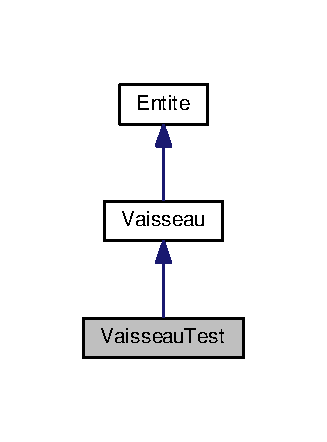
\includegraphics[width=157pt]{class_vaisseau_test__inherit__graph}
\end{center}
\end{figure}


Graphe de collaboration de Vaisseau\+Test\+:
\nopagebreak
\begin{figure}[H]
\begin{center}
\leavevmode
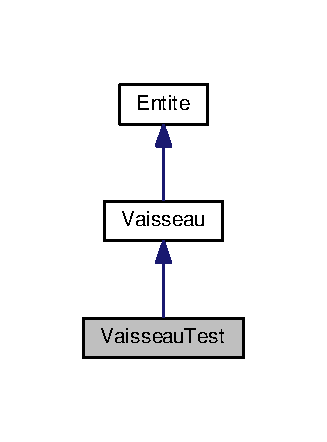
\includegraphics[width=157pt]{class_vaisseau_test__coll__graph}
\end{center}
\end{figure}
\subsection*{Fonctions membres publiques}
\begin{DoxyCompactItemize}
\item 
\hyperlink{class_vaisseau_test_acbe01fc8952d9c6fd52cbf311a92c903}{Vaisseau\+Test} ()
\begin{DoxyCompactList}\small\item\em constructeur \end{DoxyCompactList}\item 
\hyperlink{class_vaisseau_test_ada9b5788bc092ecede953248cd6133e8}{$\sim$\+Vaisseau\+Test} ()
\begin{DoxyCompactList}\small\item\em destructeur \end{DoxyCompactList}\item 
void \hyperlink{class_vaisseau_test_acf5f5ea1e9317cbc5a4c445016cd767c}{gestion} (sf\+::\+Render\+Window \&window)
\end{DoxyCompactItemize}
\subsection*{Membres hérités additionnels}


\subsection{Documentation des constructeurs et destructeur}
\mbox{\Hypertarget{class_vaisseau_test_acbe01fc8952d9c6fd52cbf311a92c903}\label{class_vaisseau_test_acbe01fc8952d9c6fd52cbf311a92c903}} 
\index{Vaisseau\+Test@{Vaisseau\+Test}!Vaisseau\+Test@{Vaisseau\+Test}}
\index{Vaisseau\+Test@{Vaisseau\+Test}!Vaisseau\+Test@{Vaisseau\+Test}}
\subsubsection{\texorpdfstring{Vaisseau\+Test()}{VaisseauTest()}}
{\footnotesize\ttfamily Vaisseau\+Test\+::\+Vaisseau\+Test (\begin{DoxyParamCaption}{ }\end{DoxyParamCaption})}



constructeur 

\mbox{\Hypertarget{class_vaisseau_test_ada9b5788bc092ecede953248cd6133e8}\label{class_vaisseau_test_ada9b5788bc092ecede953248cd6133e8}} 
\index{Vaisseau\+Test@{Vaisseau\+Test}!````~Vaisseau\+Test@{$\sim$\+Vaisseau\+Test}}
\index{````~Vaisseau\+Test@{$\sim$\+Vaisseau\+Test}!Vaisseau\+Test@{Vaisseau\+Test}}
\subsubsection{\texorpdfstring{$\sim$\+Vaisseau\+Test()}{~VaisseauTest()}}
{\footnotesize\ttfamily Vaisseau\+Test\+::$\sim$\+Vaisseau\+Test (\begin{DoxyParamCaption}{ }\end{DoxyParamCaption})}



destructeur 



\subsection{Documentation des fonctions membres}
\mbox{\Hypertarget{class_vaisseau_test_acf5f5ea1e9317cbc5a4c445016cd767c}\label{class_vaisseau_test_acf5f5ea1e9317cbc5a4c445016cd767c}} 
\index{Vaisseau\+Test@{Vaisseau\+Test}!gestion@{gestion}}
\index{gestion@{gestion}!Vaisseau\+Test@{Vaisseau\+Test}}
\subsubsection{\texorpdfstring{gestion()}{gestion()}}
{\footnotesize\ttfamily void Vaisseau\+Test\+::gestion (\begin{DoxyParamCaption}\item[{sf\+::\+Render\+Window \&}]{window }\end{DoxyParamCaption})}



La documentation de cette classe a été générée à partir des fichiers suivants \+:\begin{DoxyCompactItemize}
\item 
src/\+Vaisseau/\hyperlink{_vaisseau_test_8h}{Vaisseau\+Test.\+h}\item 
src/\+Vaisseau/\hyperlink{_vaisseau_test_8cpp}{Vaisseau\+Test.\+cpp}\end{DoxyCompactItemize}

\chapter{Documentation des fichiers}
\hypertarget{___capacites_8h}{}\section{Référence du fichier src/\+Capacites/\+\_\+\+Capacites.h}
\label{___capacites_8h}\index{src/\+Capacites/\+\_\+\+Capacites.\+h@{src/\+Capacites/\+\_\+\+Capacites.\+h}}
{\ttfamily \#include \char`\"{}Cap\+Test.\+h\char`\"{}}\newline
{\ttfamily \#include \char`\"{}Cap\+Piou.\+h\char`\"{}}\newline
{\ttfamily \#include \char`\"{}Cap\+Dash.\+h\char`\"{}}\newline
Graphe des dépendances par inclusion de \+\_\+\+Capacites.\+h\+:
\nopagebreak
\begin{figure}[H]
\begin{center}
\leavevmode
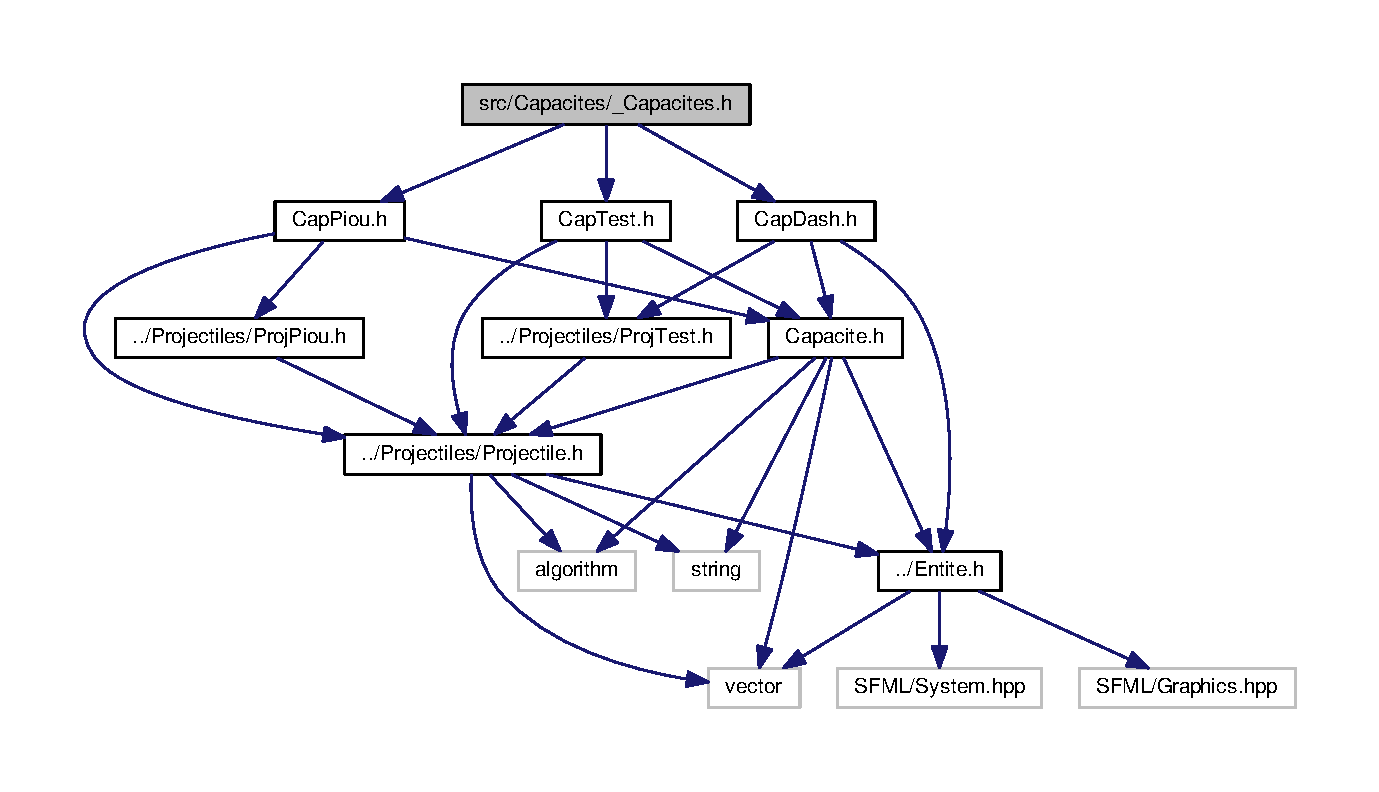
\includegraphics[width=350pt]{___capacites_8h__incl}
\end{center}
\end{figure}
Ce graphe montre quels fichiers incluent directement ou indirectement ce fichier \+:
\nopagebreak
\begin{figure}[H]
\begin{center}
\leavevmode
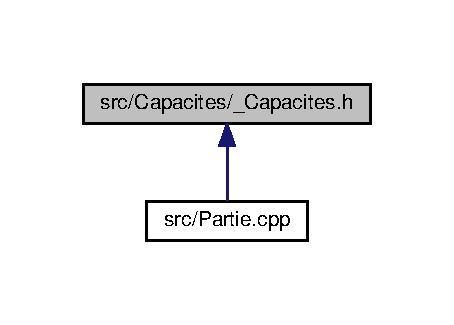
\includegraphics[width=218pt]{___capacites_8h__dep__incl}
\end{center}
\end{figure}

\hypertarget{_capacite_8cpp}{}\section{Référence du fichier src/\+Capacite.cpp}
\label{_capacite_8cpp}\index{src/\+Capacite.\+cpp@{src/\+Capacite.\+cpp}}
{\ttfamily \#include $<$vector$>$}\newline
{\ttfamily \#include $<$string$>$}\newline
{\ttfamily \#include $<$algorithm$>$}\newline
{\ttfamily \#include \char`\"{}Capacite.\+h\char`\"{}}\newline
{\ttfamily \#include \char`\"{}Vaisseau.\+h\char`\"{}}\newline
{\ttfamily \#include \char`\"{}Projectile.\+h\char`\"{}}\newline
Graphe des dépendances par inclusion de Capacite.\+cpp\+:\nopagebreak
\begin{figure}[H]
\begin{center}
\leavevmode
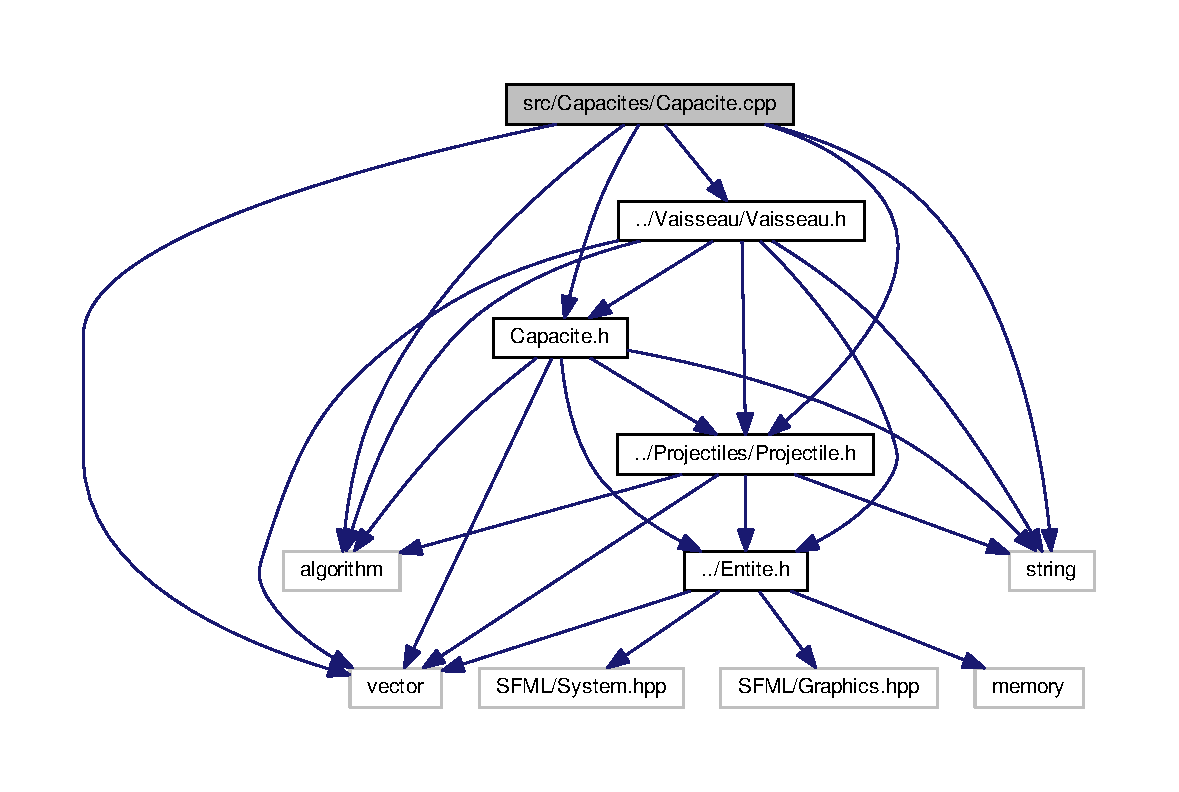
\includegraphics[width=350pt]{_capacite_8cpp__incl}
\end{center}
\end{figure}

\hypertarget{_capacite_8h}{}\section{Référence du fichier src/\+Capacite.h}
\label{_capacite_8h}\index{src/\+Capacite.\+h@{src/\+Capacite.\+h}}
\subsection*{Classes}
\begin{DoxyCompactItemize}
\item 
class \hyperlink{class_capacite}{Capacite}
\begin{DoxyCompactList}\small\item\em Classe virtuelle qui définit la structure générale d\textquotesingle{}une capacité \end{DoxyCompactList}\end{DoxyCompactItemize}

\hypertarget{_cap_aim_bot_8cpp}{}\section{Référence du fichier src/\+Capacites/\+Cap\+Aim\+Bot.cpp}
\label{_cap_aim_bot_8cpp}\index{src/\+Capacites/\+Cap\+Aim\+Bot.\+cpp@{src/\+Capacites/\+Cap\+Aim\+Bot.\+cpp}}
{\ttfamily \#include \char`\"{}Cap\+Aim\+Bot.\+h\char`\"{}}\newline
{\ttfamily \#include \char`\"{}Cap\+Missile.\+h\char`\"{}}\newline
Graphe des dépendances par inclusion de Cap\+Aim\+Bot.\+cpp\+:
% FIG 0

\hypertarget{_cap_aim_bot_8h}{}\section{src/\+Capacites/\+Cap\+Aim\+Bot.h File Reference}
\label{_cap_aim_bot_8h}\index{src/\+Capacites/\+Cap\+Aim\+Bot.\+h@{src/\+Capacites/\+Cap\+Aim\+Bot.\+h}}
{\ttfamily \#include \char`\"{}Capacite.\+h\char`\"{}}\newline
\subsection*{Classes}
\begin{DoxyCompactItemize}
\item 
class \mbox{\hyperlink{class_cap_aim_bot}{Cap\+Aim\+Bot}}
\begin{DoxyCompactList}\small\item\em donne visée auto à un skill (missile) \end{DoxyCompactList}\end{DoxyCompactItemize}

\hypertarget{_cap_bismillah_beam_8cpp}{}\section{Référence du fichier src/\+Capacites/\+Cap\+Bismillah\+Beam.cpp}
\label{_cap_bismillah_beam_8cpp}\index{src/\+Capacites/\+Cap\+Bismillah\+Beam.\+cpp@{src/\+Capacites/\+Cap\+Bismillah\+Beam.\+cpp}}
{\ttfamily \#include \char`\"{}Cap\+Bismillah\+Beam.\+h\char`\"{}}\newline
{\ttfamily \#include \char`\"{}../\+Projectiles/\+Proj\+Bismillah.\+h\char`\"{}}\newline
Graphe des dépendances par inclusion de Cap\+Bismillah\+Beam.\+cpp\+:
% FIG 0

\hypertarget{_cap_bismillah_beam_8h}{}\section{src/\+Capacites/\+Cap\+Bismillah\+Beam.h File Reference}
\label{_cap_bismillah_beam_8h}\index{src/\+Capacites/\+Cap\+Bismillah\+Beam.\+h@{src/\+Capacites/\+Cap\+Bismillah\+Beam.\+h}}
{\ttfamily \#include \char`\"{}Capacite.\+h\char`\"{}}\newline
\subsection*{Classes}
\begin{DoxyCompactItemize}
\item 
class \mbox{\hyperlink{class_cap_bismillah}{Cap\+Bismillah}}
\end{DoxyCompactItemize}

\hypertarget{_cap_boing_8cpp}{}\section{Référence du fichier src/\+Capacites/\+Cap\+Boing.cpp}
\label{_cap_boing_8cpp}\index{src/\+Capacites/\+Cap\+Boing.\+cpp@{src/\+Capacites/\+Cap\+Boing.\+cpp}}
{\ttfamily \#include \char`\"{}Cap\+Boing.\+h\char`\"{}}\newline
{\ttfamily \#include \char`\"{}Cap\+Dash.\+h\char`\"{}}\newline
Graphe des dépendances par inclusion de Cap\+Boing.\+cpp\+:
% FIG 0

\hypertarget{_cap_boing_8h}{}\section{src/\+Capacites/\+Cap\+Boing.h File Reference}
\label{_cap_boing_8h}\index{src/\+Capacites/\+Cap\+Boing.\+h@{src/\+Capacites/\+Cap\+Boing.\+h}}
{\ttfamily \#include \char`\"{}Capacite.\+h\char`\"{}}\newline
{\ttfamily \#include \char`\"{}../\+Projectiles/\+Projectile.\+h\char`\"{}}\newline
{\ttfamily \#include \char`\"{}../\+Projectiles/\+Proj\+Boing.\+h\char`\"{}}\newline
\subsection*{Classes}
\begin{DoxyCompactItemize}
\item 
class \mbox{\hyperlink{class_cap_boing}{Cap\+Boing}}
\begin{DoxyCompactList}\small\item\em Classe Capacité de test. \end{DoxyCompactList}\end{DoxyCompactItemize}

\hypertarget{_cap_bouclier_rond_8cpp}{}\section{Référence du fichier src/\+Capacites/\+Cap\+Bouclier\+Rond.cpp}
\label{_cap_bouclier_rond_8cpp}\index{src/\+Capacites/\+Cap\+Bouclier\+Rond.\+cpp@{src/\+Capacites/\+Cap\+Bouclier\+Rond.\+cpp}}
{\ttfamily \#include \char`\"{}Cap\+Bouclier\+Rond.\+h\char`\"{}}\newline
Graphe des dépendances par inclusion de Cap\+Bouclier\+Rond.\+cpp\+:
% FIG 0

\hypertarget{_cap_bouclier_rond_8h}{}\section{Référence du fichier src/\+Capacites/\+Cap\+Bouclier\+Rond.h}
\label{_cap_bouclier_rond_8h}\index{src/\+Capacites/\+Cap\+Bouclier\+Rond.\+h@{src/\+Capacites/\+Cap\+Bouclier\+Rond.\+h}}
{\ttfamily \#include \char`\"{}Capacite.\+h\char`\"{}}\newline
{\ttfamily \#include \char`\"{}../\+Projectiles/\+Projectile.\+h\char`\"{}}\newline
{\ttfamily \#include \char`\"{}../\+Projectiles/\+Proj\+Bouclier\+Rond.\+h\char`\"{}}\newline
Graphe des dépendances par inclusion de Cap\+Bouclier\+Rond.\+h\+:
% FIG 0
Ce graphe montre quels fichiers incluent directement ou indirectement ce fichier \+:
% FIG 1
\subsection*{Classes}
\begin{DoxyCompactItemize}
\item 
class \hyperlink{class_cap_bouclier_rond}{Cap\+Bouclier\+Rond}
\begin{DoxyCompactList}\small\item\em bouclier circulaire avec x PB \end{DoxyCompactList}\end{DoxyCompactItemize}

\hypertarget{_cap_dash_8cpp}{}\section{Référence du fichier src/\+Cap\+Dash.cpp}
\label{_cap_dash_8cpp}\index{src/\+Cap\+Dash.\+cpp@{src/\+Cap\+Dash.\+cpp}}
{\ttfamily \#include \char`\"{}Cap\+Dash.\+h\char`\"{}}\newline
Graphe des dépendances par inclusion de Cap\+Dash.\+cpp\+:\nopagebreak
\begin{figure}[H]
\begin{center}
\leavevmode
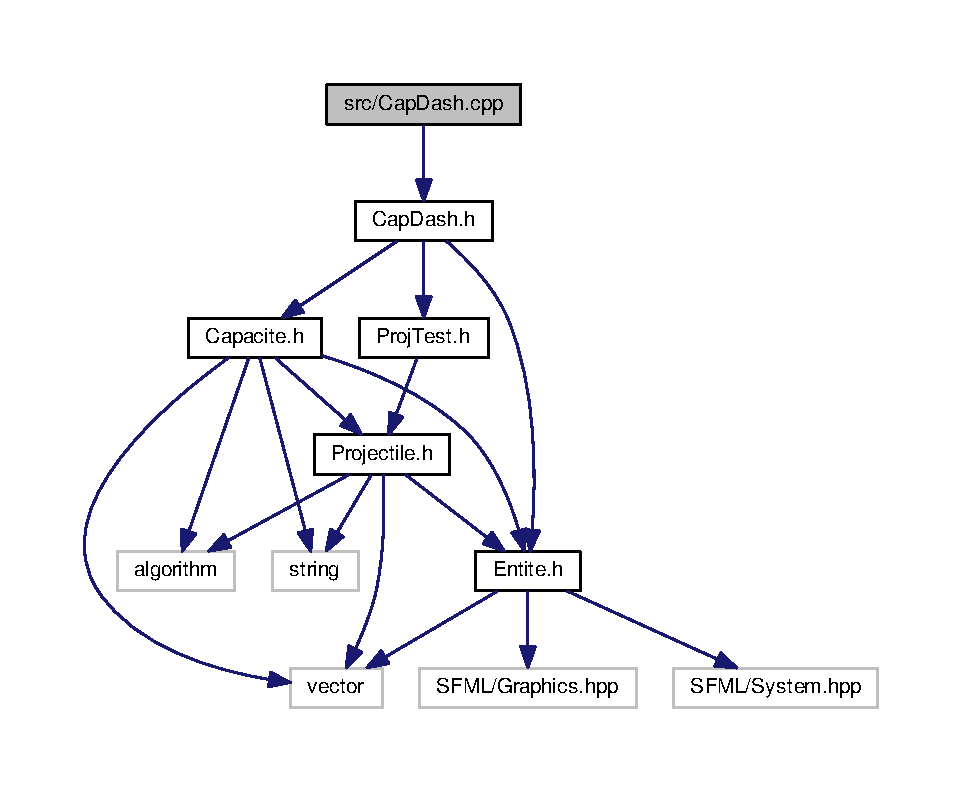
\includegraphics[width=350pt]{_cap_dash_8cpp__incl}
\end{center}
\end{figure}

\hypertarget{_cap_dash_8h}{}\section{Référence du fichier src/\+Capacites/\+Cap\+Dash.h}
\label{_cap_dash_8h}\index{src/\+Capacites/\+Cap\+Dash.\+h@{src/\+Capacites/\+Cap\+Dash.\+h}}
{\ttfamily \#include \char`\"{}Capacite.\+h\char`\"{}}\newline
{\ttfamily \#include \char`\"{}../\+Entite.\+h\char`\"{}}\newline
{\ttfamily \#include \char`\"{}../\+Projectiles/\+Proj\+Test.\+h\char`\"{}}\newline
Graphe des dépendances par inclusion de Cap\+Dash.\+h\+:
\nopagebreak
\begin{figure}[H]
\begin{center}
\leavevmode
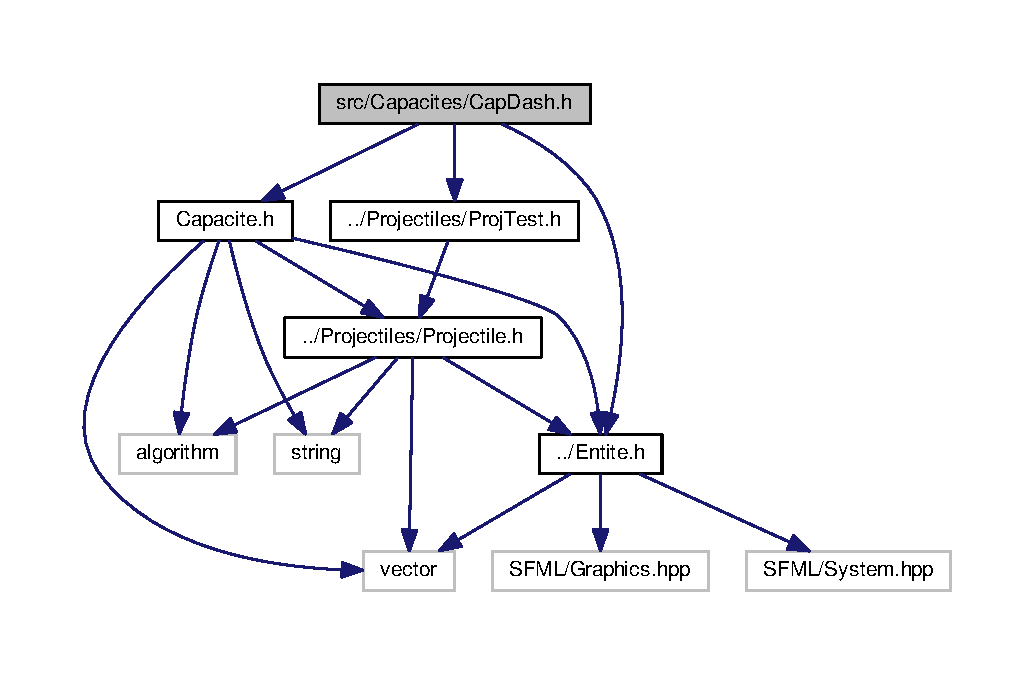
\includegraphics[width=350pt]{_cap_dash_8h__incl}
\end{center}
\end{figure}
Ce graphe montre quels fichiers incluent directement ou indirectement ce fichier \+:
\nopagebreak
\begin{figure}[H]
\begin{center}
\leavevmode
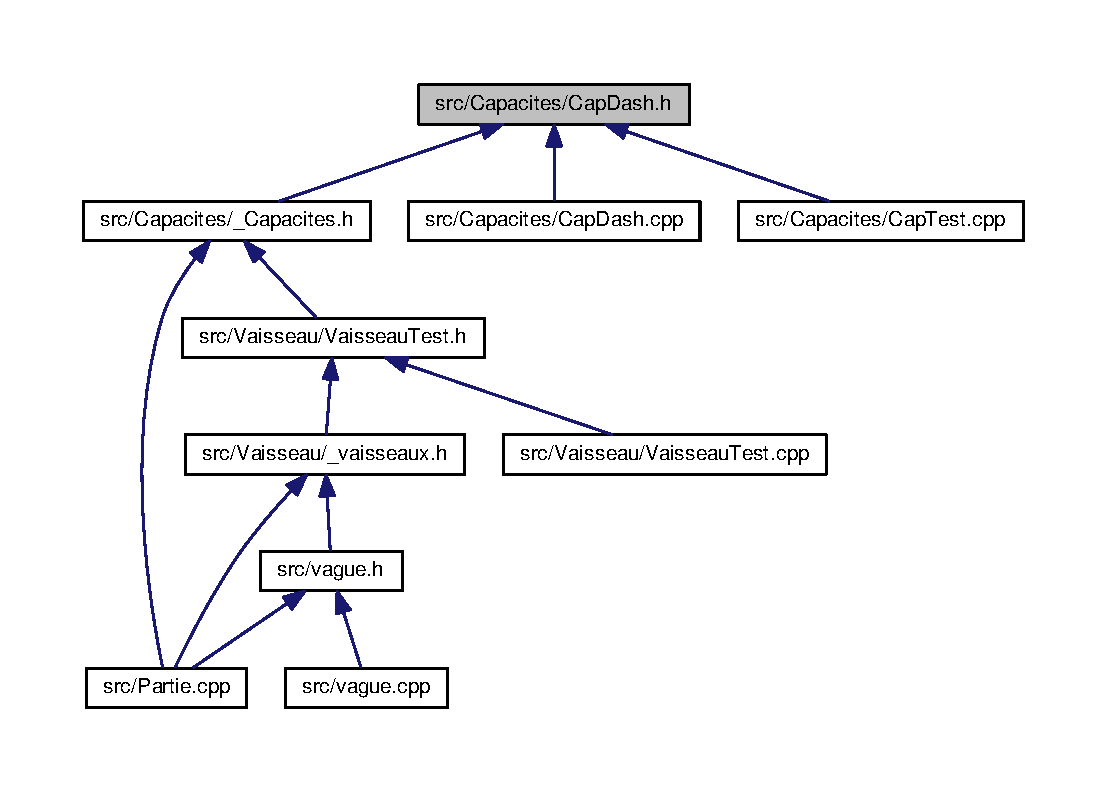
\includegraphics[width=350pt]{_cap_dash_8h__dep__incl}
\end{center}
\end{figure}
\subsection*{Classes}
\begin{DoxyCompactItemize}
\item 
class \hyperlink{class_cap_dash}{Cap\+Dash}
\end{DoxyCompactItemize}

\hypertarget{_cap_missile_8cpp}{}\section{src/\+Capacites/\+Cap\+Missile.cpp File Reference}
\label{_cap_missile_8cpp}\index{src/\+Capacites/\+Cap\+Missile.\+cpp@{src/\+Capacites/\+Cap\+Missile.\+cpp}}
{\ttfamily \#include \char`\"{}Cap\+Missile.\+h\char`\"{}}\newline

\hypertarget{_cap_missile_8h}{}\section{Référence du fichier src/\+Capacites/\+Cap\+Missile.h}
\label{_cap_missile_8h}\index{src/\+Capacites/\+Cap\+Missile.\+h@{src/\+Capacites/\+Cap\+Missile.\+h}}
{\ttfamily \#include \char`\"{}Capacite.\+h\char`\"{}}\newline
{\ttfamily \#include \char`\"{}../\+Projectiles/\+Proj\+Missile.\+h\char`\"{}}\newline
Graphe des dépendances par inclusion de Cap\+Missile.\+h\+:
% FIG 0
Ce graphe montre quels fichiers incluent directement ou indirectement ce fichier \+:
% FIG 1
\subsection*{Classes}
\begin{DoxyCompactItemize}
\item 
class \hyperlink{class_cap_missile}{Cap\+Missile}
\begin{DoxyCompactList}\small\item\em Classe Capacité de base. \end{DoxyCompactList}\end{DoxyCompactItemize}

\hypertarget{_cap_piou_8cpp}{}\section{Référence du fichier src/\+Cap\+Piou.cpp}
\label{_cap_piou_8cpp}\index{src/\+Cap\+Piou.\+cpp@{src/\+Cap\+Piou.\+cpp}}
{\ttfamily \#include \char`\"{}Cap\+Piou.\+h\char`\"{}}\newline
Graphe des dépendances par inclusion de Cap\+Piou.\+cpp\+:\nopagebreak
\begin{figure}[H]
\begin{center}
\leavevmode
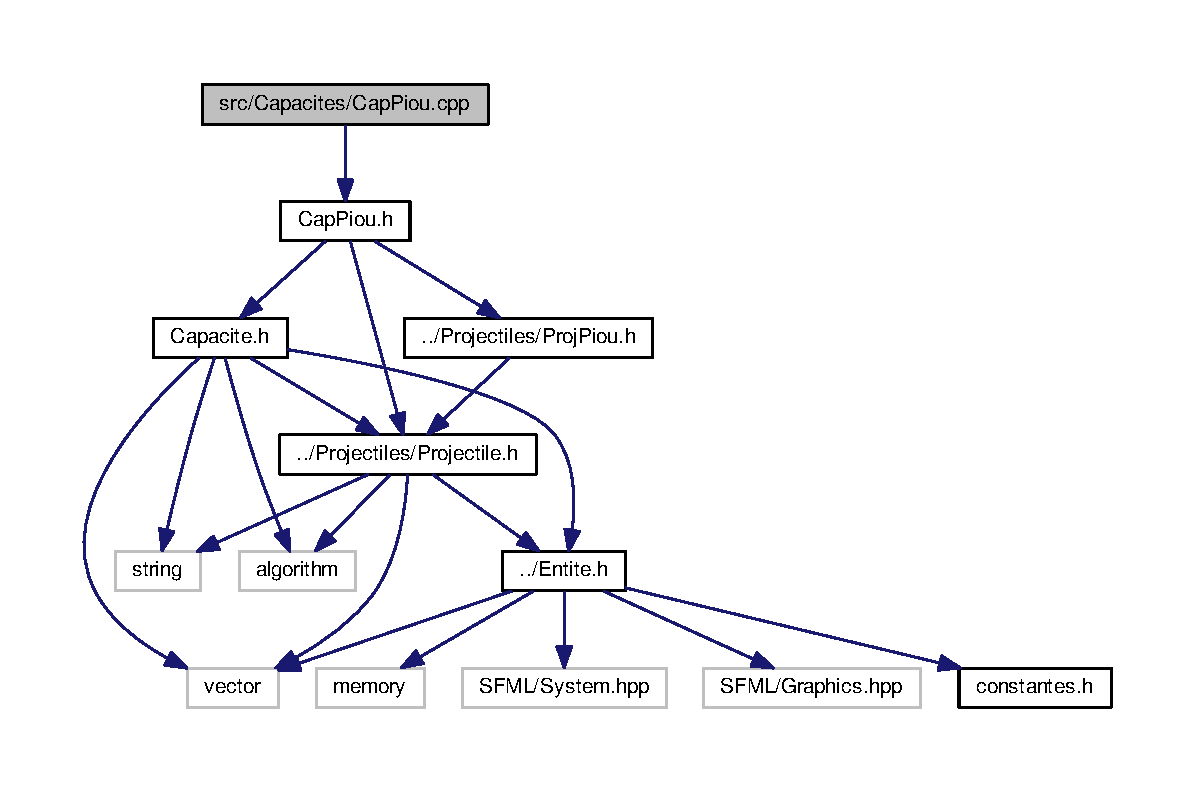
\includegraphics[width=350pt]{_cap_piou_8cpp__incl}
\end{center}
\end{figure}

\hypertarget{_cap_piou_8h}{}\section{Référence du fichier src/\+Capacites/\+Cap\+Piou.h}
\label{_cap_piou_8h}\index{src/\+Capacites/\+Cap\+Piou.\+h@{src/\+Capacites/\+Cap\+Piou.\+h}}
{\ttfamily \#include \char`\"{}Capacite.\+h\char`\"{}}\newline
{\ttfamily \#include \char`\"{}../\+Projectiles/\+Projectile.\+h\char`\"{}}\newline
{\ttfamily \#include \char`\"{}../\+Projectiles/\+Proj\+Piou.\+h\char`\"{}}\newline
Graphe des dépendances par inclusion de Cap\+Piou.\+h\+:\nopagebreak
\begin{figure}[H]
\begin{center}
\leavevmode
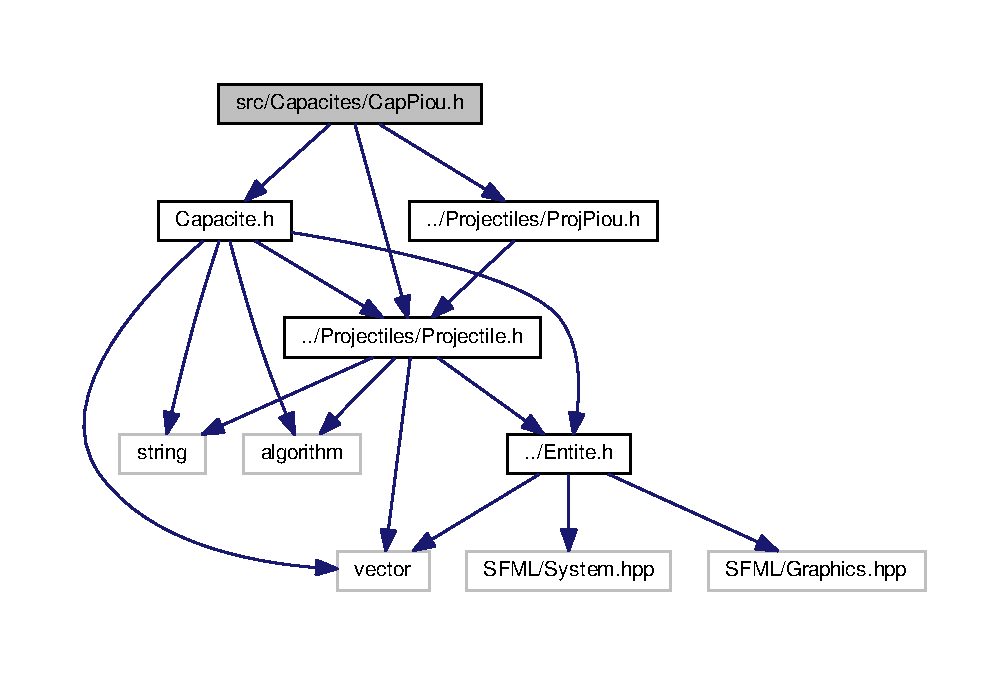
\includegraphics[width=350pt]{_cap_piou_8h__incl}
\end{center}
\end{figure}
Ce graphe montre quels fichiers incluent directement ou indirectement ce fichier \+:\nopagebreak
\begin{figure}[H]
\begin{center}
\leavevmode
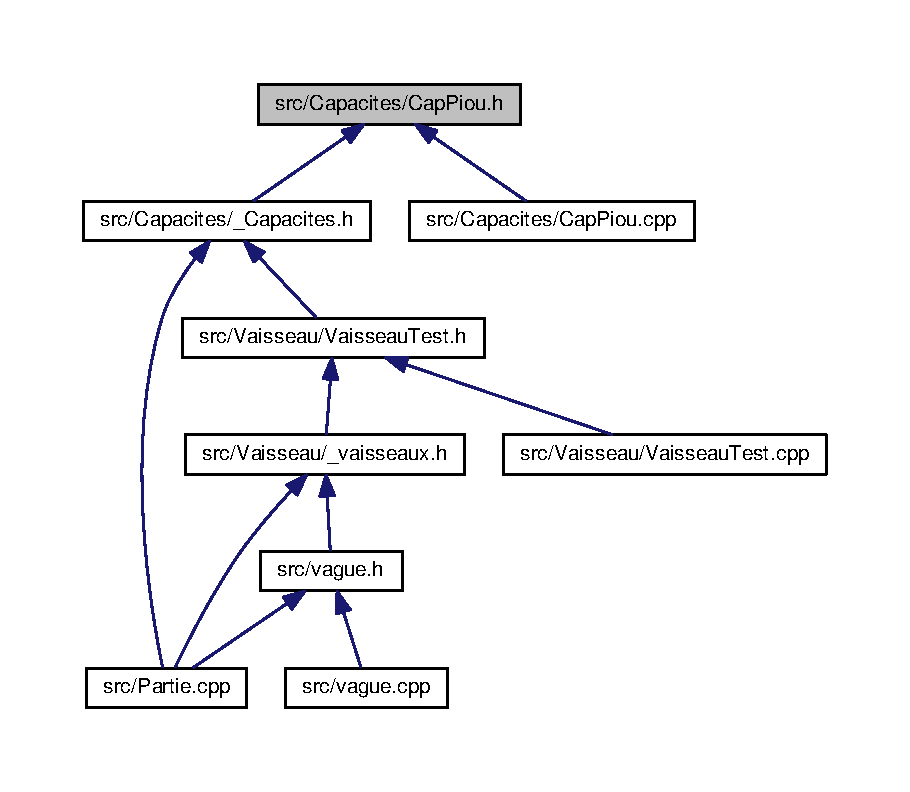
\includegraphics[width=350pt]{_cap_piou_8h__dep__incl}
\end{center}
\end{figure}
\subsection*{Classes}
\begin{DoxyCompactItemize}
\item 
class \hyperlink{class_cap_piou}{Cap\+Piou}
\begin{DoxyCompactList}\small\item\em Classe Capacité de base. \end{DoxyCompactList}\end{DoxyCompactItemize}

\hypertarget{constantes_8h}{}\section{Référence du fichier src/constantes.h}
\label{constantes_8h}\index{src/constantes.\+h@{src/constantes.\+h}}
Ce graphe montre quels fichiers incluent directement ou indirectement ce fichier \+:
\nopagebreak
\begin{figure}[H]
\begin{center}
\leavevmode
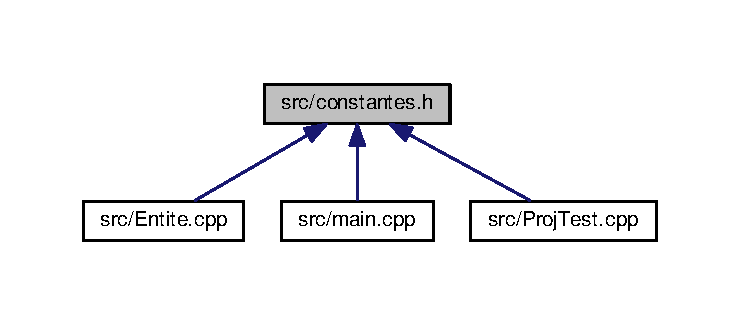
\includegraphics[width=350pt]{constantes_8h__dep__incl}
\end{center}
\end{figure}
\subsection*{Macros}
\begin{DoxyCompactItemize}
\item 
\#define \hyperlink{constantes_8h_a078285dfdd5f8d9caa79aeb3f4eb0a1f}{E\+C\+R\+A\+N\+\_\+L}~1024
\item 
\#define \hyperlink{constantes_8h_a75c426da06c2ec9164baaf36a262fa07}{E\+C\+R\+A\+N\+\_\+H}~768
\end{DoxyCompactItemize}


\subsection{Documentation des macros}
\mbox{\Hypertarget{constantes_8h_a75c426da06c2ec9164baaf36a262fa07}\label{constantes_8h_a75c426da06c2ec9164baaf36a262fa07}} 
\index{constantes.\+h@{constantes.\+h}!E\+C\+R\+A\+N\+\_\+H@{E\+C\+R\+A\+N\+\_\+H}}
\index{E\+C\+R\+A\+N\+\_\+H@{E\+C\+R\+A\+N\+\_\+H}!constantes.\+h@{constantes.\+h}}
\subsubsection{\texorpdfstring{E\+C\+R\+A\+N\+\_\+H}{ECRAN\_H}}
{\footnotesize\ttfamily \#define E\+C\+R\+A\+N\+\_\+H~768}

\mbox{\Hypertarget{constantes_8h_a078285dfdd5f8d9caa79aeb3f4eb0a1f}\label{constantes_8h_a078285dfdd5f8d9caa79aeb3f4eb0a1f}} 
\index{constantes.\+h@{constantes.\+h}!E\+C\+R\+A\+N\+\_\+L@{E\+C\+R\+A\+N\+\_\+L}}
\index{E\+C\+R\+A\+N\+\_\+L@{E\+C\+R\+A\+N\+\_\+L}!constantes.\+h@{constantes.\+h}}
\subsubsection{\texorpdfstring{E\+C\+R\+A\+N\+\_\+L}{ECRAN\_L}}
{\footnotesize\ttfamily \#define E\+C\+R\+A\+N\+\_\+L~1024}


\hypertarget{_entite_8cpp}{}\section{Référence du fichier src/\+Entite.cpp}
\label{_entite_8cpp}\index{src/\+Entite.\+cpp@{src/\+Entite.\+cpp}}
{\ttfamily \#include \char`\"{}Entite.\+h\char`\"{}}\newline
{\ttfamily \#include \char`\"{}Utilitaires/\+Collision.\+h\char`\"{}}\newline
{\ttfamily \#include \char`\"{}constantes.\+h\char`\"{}}\newline
{\ttfamily \#include $<$cmath$>$}\newline
Graphe des dépendances par inclusion de Entite.\+cpp\+:
% FIG 0
\subsection*{Fonctions}
\begin{DoxyCompactItemize}
\item 
bool \hyperlink{_entite_8cpp_ac85cf277aaeb8a314734c1fa5f35e3be}{collision} (const \hyperlink{class_entite}{Entite} \&e1, const \hyperlink{class_entite}{Entite} \&e2)
\end{DoxyCompactItemize}


\subsection{Documentation des fonctions}
\mbox{\Hypertarget{_entite_8cpp_ac85cf277aaeb8a314734c1fa5f35e3be}\label{_entite_8cpp_ac85cf277aaeb8a314734c1fa5f35e3be}} 
\index{Entite.\+cpp@{Entite.\+cpp}!collision@{collision}}
\index{collision@{collision}!Entite.\+cpp@{Entite.\+cpp}}
\subsubsection{\texorpdfstring{collision()}{collision()}}
{\footnotesize\ttfamily bool collision (\begin{DoxyParamCaption}\item[{const \hyperlink{class_entite}{Entite} \&}]{e1,  }\item[{const \hyperlink{class_entite}{Entite} \&}]{e2 }\end{DoxyParamCaption})}


\hypertarget{_entite_8h}{}\section{Référence du fichier src/\+Entite.h}
\label{_entite_8h}\index{src/\+Entite.\+h@{src/\+Entite.\+h}}
{\ttfamily \#include $<$vector$>$}\newline
{\ttfamily \#include $<$memory$>$}\newline
{\ttfamily \#include $<$S\+F\+M\+L/\+System.\+hpp$>$}\newline
{\ttfamily \#include $<$S\+F\+M\+L/\+Graphics.\+hpp$>$}\newline
Graphe des dépendances par inclusion de Entite.\+h\+:\nopagebreak
\begin{figure}[H]
\begin{center}
\leavevmode
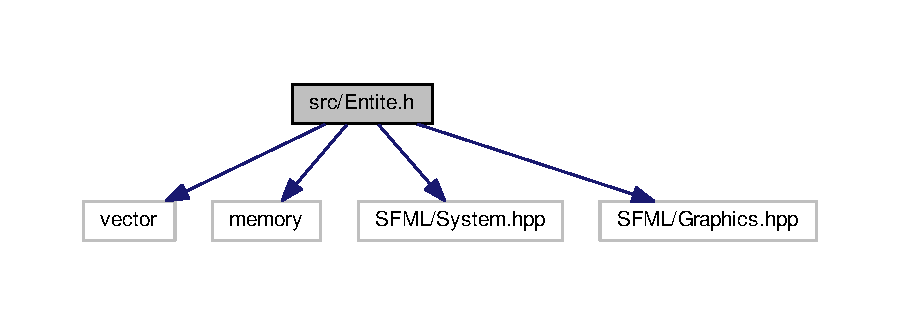
\includegraphics[width=350pt]{_entite_8h__incl}
\end{center}
\end{figure}
Ce graphe montre quels fichiers incluent directement ou indirectement ce fichier \+:\nopagebreak
\begin{figure}[H]
\begin{center}
\leavevmode
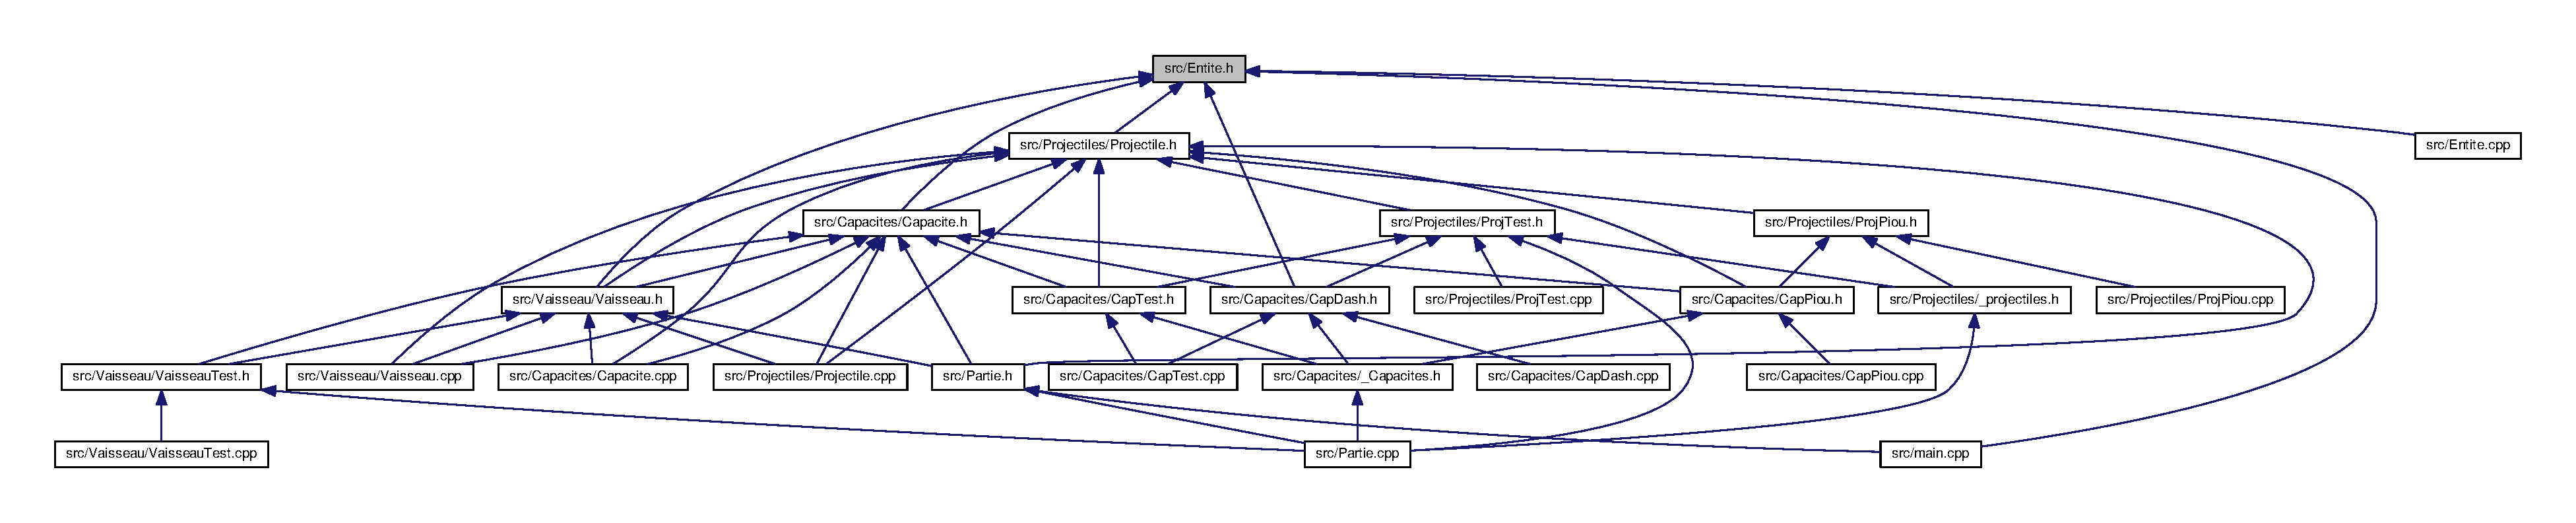
\includegraphics[width=350pt]{_entite_8h__dep__incl}
\end{center}
\end{figure}
\subsection*{Classes}
\begin{DoxyCompactItemize}
\item 
class \hyperlink{class_entite}{Entite}
\begin{DoxyCompactList}\small\item\em Classe virtuelle qui définit une entité \end{DoxyCompactList}\end{DoxyCompactItemize}

\hypertarget{bindings_8cpp}{}\section{Référence du fichier src/\+Interface/bindings.cpp}
\label{bindings_8cpp}\index{src/\+Interface/bindings.\+cpp@{src/\+Interface/bindings.\+cpp}}
{\ttfamily \#include \char`\"{}bindings.\+h\char`\"{}}\newline
Graphe des dépendances par inclusion de bindings.\+cpp\+:\nopagebreak
\begin{figure}[H]
\begin{center}
\leavevmode
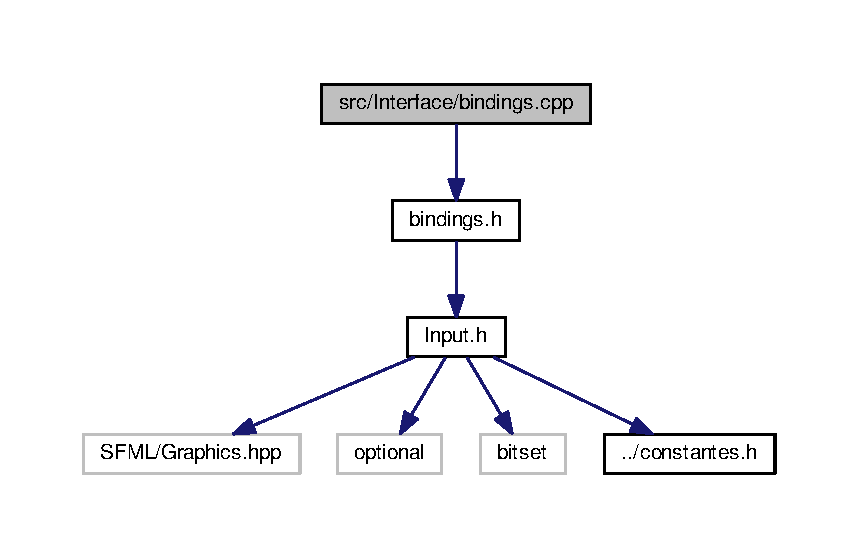
\includegraphics[width=350pt]{bindings_8cpp__incl}
\end{center}
\end{figure}
\subsection*{Fonctions}
\begin{DoxyCompactItemize}
\item 
void \hyperlink{bindings_8cpp_a33f9529428adfaa552e681749b796076}{set\+\_\+keyboard\+\_\+default\+\_\+binding} (\hyperlink{_input_8h_a5588d60d674991c719a8df848313e966}{Input} \&in)
\item 
void \hyperlink{bindings_8cpp_a6c343c7a09bb1d08e2a0f6e97773f57b}{set\+\_\+mouse\+\_\+default\+\_\+binding} (\hyperlink{_input_8h_a5588d60d674991c719a8df848313e966}{Input} \&in)
\item 
void \hyperlink{bindings_8cpp_a5249f510d79fb689561e3e4de1bba0d4}{set\+\_\+joypad\+\_\+default\+\_\+binding} (\hyperlink{_input_8h_a5588d60d674991c719a8df848313e966}{Input} \&in)
\end{DoxyCompactItemize}


\subsection{Documentation des fonctions}
\mbox{\Hypertarget{bindings_8cpp_a5249f510d79fb689561e3e4de1bba0d4}\label{bindings_8cpp_a5249f510d79fb689561e3e4de1bba0d4}} 
\index{bindings.\+cpp@{bindings.\+cpp}!set\+\_\+joypad\+\_\+default\+\_\+binding@{set\+\_\+joypad\+\_\+default\+\_\+binding}}
\index{set\+\_\+joypad\+\_\+default\+\_\+binding@{set\+\_\+joypad\+\_\+default\+\_\+binding}!bindings.\+cpp@{bindings.\+cpp}}
\subsubsection{\texorpdfstring{set\+\_\+joypad\+\_\+default\+\_\+binding()}{set\_joypad\_default\_binding()}}
{\footnotesize\ttfamily void set\+\_\+joypad\+\_\+default\+\_\+binding (\begin{DoxyParamCaption}\item[{\hyperlink{_input_8h_a5588d60d674991c719a8df848313e966}{Input} \&}]{in }\end{DoxyParamCaption})}

\mbox{\Hypertarget{bindings_8cpp_a33f9529428adfaa552e681749b796076}\label{bindings_8cpp_a33f9529428adfaa552e681749b796076}} 
\index{bindings.\+cpp@{bindings.\+cpp}!set\+\_\+keyboard\+\_\+default\+\_\+binding@{set\+\_\+keyboard\+\_\+default\+\_\+binding}}
\index{set\+\_\+keyboard\+\_\+default\+\_\+binding@{set\+\_\+keyboard\+\_\+default\+\_\+binding}!bindings.\+cpp@{bindings.\+cpp}}
\subsubsection{\texorpdfstring{set\+\_\+keyboard\+\_\+default\+\_\+binding()}{set\_keyboard\_default\_binding()}}
{\footnotesize\ttfamily void set\+\_\+keyboard\+\_\+default\+\_\+binding (\begin{DoxyParamCaption}\item[{\hyperlink{_input_8h_a5588d60d674991c719a8df848313e966}{Input} \&}]{in }\end{DoxyParamCaption})}

\mbox{\Hypertarget{bindings_8cpp_a6c343c7a09bb1d08e2a0f6e97773f57b}\label{bindings_8cpp_a6c343c7a09bb1d08e2a0f6e97773f57b}} 
\index{bindings.\+cpp@{bindings.\+cpp}!set\+\_\+mouse\+\_\+default\+\_\+binding@{set\+\_\+mouse\+\_\+default\+\_\+binding}}
\index{set\+\_\+mouse\+\_\+default\+\_\+binding@{set\+\_\+mouse\+\_\+default\+\_\+binding}!bindings.\+cpp@{bindings.\+cpp}}
\subsubsection{\texorpdfstring{set\+\_\+mouse\+\_\+default\+\_\+binding()}{set\_mouse\_default\_binding()}}
{\footnotesize\ttfamily void set\+\_\+mouse\+\_\+default\+\_\+binding (\begin{DoxyParamCaption}\item[{\hyperlink{_input_8h_a5588d60d674991c719a8df848313e966}{Input} \&}]{in }\end{DoxyParamCaption})}


\hypertarget{bindings_8h}{}\section{src/\+Interface/bindings.h File Reference}
\label{bindings_8h}\index{src/\+Interface/bindings.\+h@{src/\+Interface/bindings.\+h}}
{\ttfamily \#include \char`\"{}Input.\+h\char`\"{}}\newline
\subsection*{Functions}
\begin{DoxyCompactItemize}
\item 
void \mbox{\hyperlink{bindings_8h_a33f9529428adfaa552e681749b796076}{set\+\_\+keyboard\+\_\+default\+\_\+binding}} (\mbox{\hyperlink{_input_8h_a5588d60d674991c719a8df848313e966}{Input}} \&in)
\item 
void \mbox{\hyperlink{bindings_8h_a17708a73bad94fe511a43e063956565d}{set\+\_\+keyboard\+\_\+default\+\_\+binding\+\_\+2}} (\mbox{\hyperlink{_input_8h_a5588d60d674991c719a8df848313e966}{Input}} \&in)
\item 
void \mbox{\hyperlink{bindings_8h_a6c343c7a09bb1d08e2a0f6e97773f57b}{set\+\_\+mouse\+\_\+default\+\_\+binding}} (\mbox{\hyperlink{_input_8h_a5588d60d674991c719a8df848313e966}{Input}} \&in)
\item 
void \mbox{\hyperlink{bindings_8h_a5249f510d79fb689561e3e4de1bba0d4}{set\+\_\+joypad\+\_\+default\+\_\+binding}} (\mbox{\hyperlink{_input_8h_a5588d60d674991c719a8df848313e966}{Input}} \&in)
\end{DoxyCompactItemize}


\subsection{Function Documentation}
\mbox{\Hypertarget{bindings_8h_a5249f510d79fb689561e3e4de1bba0d4}\label{bindings_8h_a5249f510d79fb689561e3e4de1bba0d4}} 
\index{bindings.\+h@{bindings.\+h}!set\+\_\+joypad\+\_\+default\+\_\+binding@{set\+\_\+joypad\+\_\+default\+\_\+binding}}
\index{set\+\_\+joypad\+\_\+default\+\_\+binding@{set\+\_\+joypad\+\_\+default\+\_\+binding}!bindings.\+h@{bindings.\+h}}
\subsubsection{\texorpdfstring{set\+\_\+joypad\+\_\+default\+\_\+binding()}{set\_joypad\_default\_binding()}}
{\footnotesize\ttfamily void set\+\_\+joypad\+\_\+default\+\_\+binding (\begin{DoxyParamCaption}\item[{\mbox{\hyperlink{_input_8h_a5588d60d674991c719a8df848313e966}{Input}} \&}]{in }\end{DoxyParamCaption})}

\mbox{\Hypertarget{bindings_8h_a33f9529428adfaa552e681749b796076}\label{bindings_8h_a33f9529428adfaa552e681749b796076}} 
\index{bindings.\+h@{bindings.\+h}!set\+\_\+keyboard\+\_\+default\+\_\+binding@{set\+\_\+keyboard\+\_\+default\+\_\+binding}}
\index{set\+\_\+keyboard\+\_\+default\+\_\+binding@{set\+\_\+keyboard\+\_\+default\+\_\+binding}!bindings.\+h@{bindings.\+h}}
\subsubsection{\texorpdfstring{set\+\_\+keyboard\+\_\+default\+\_\+binding()}{set\_keyboard\_default\_binding()}}
{\footnotesize\ttfamily void set\+\_\+keyboard\+\_\+default\+\_\+binding (\begin{DoxyParamCaption}\item[{\mbox{\hyperlink{_input_8h_a5588d60d674991c719a8df848313e966}{Input}} \&}]{in }\end{DoxyParamCaption})}

\mbox{\Hypertarget{bindings_8h_a17708a73bad94fe511a43e063956565d}\label{bindings_8h_a17708a73bad94fe511a43e063956565d}} 
\index{bindings.\+h@{bindings.\+h}!set\+\_\+keyboard\+\_\+default\+\_\+binding\+\_\+2@{set\+\_\+keyboard\+\_\+default\+\_\+binding\+\_\+2}}
\index{set\+\_\+keyboard\+\_\+default\+\_\+binding\+\_\+2@{set\+\_\+keyboard\+\_\+default\+\_\+binding\+\_\+2}!bindings.\+h@{bindings.\+h}}
\subsubsection{\texorpdfstring{set\+\_\+keyboard\+\_\+default\+\_\+binding\+\_\+2()}{set\_keyboard\_default\_binding\_2()}}
{\footnotesize\ttfamily void set\+\_\+keyboard\+\_\+default\+\_\+binding\+\_\+2 (\begin{DoxyParamCaption}\item[{\mbox{\hyperlink{_input_8h_a5588d60d674991c719a8df848313e966}{Input}} \&}]{in }\end{DoxyParamCaption})}

\mbox{\Hypertarget{bindings_8h_a6c343c7a09bb1d08e2a0f6e97773f57b}\label{bindings_8h_a6c343c7a09bb1d08e2a0f6e97773f57b}} 
\index{bindings.\+h@{bindings.\+h}!set\+\_\+mouse\+\_\+default\+\_\+binding@{set\+\_\+mouse\+\_\+default\+\_\+binding}}
\index{set\+\_\+mouse\+\_\+default\+\_\+binding@{set\+\_\+mouse\+\_\+default\+\_\+binding}!bindings.\+h@{bindings.\+h}}
\subsubsection{\texorpdfstring{set\+\_\+mouse\+\_\+default\+\_\+binding()}{set\_mouse\_default\_binding()}}
{\footnotesize\ttfamily void set\+\_\+mouse\+\_\+default\+\_\+binding (\begin{DoxyParamCaption}\item[{\mbox{\hyperlink{_input_8h_a5588d60d674991c719a8df848313e966}{Input}} \&}]{in }\end{DoxyParamCaption})}


\hypertarget{_bouton_capacite_8h}{}\section{Référence du fichier src/\+Interface/\+Bouton\+Capacite.h}
\label{_bouton_capacite_8h}\index{src/\+Interface/\+Bouton\+Capacite.\+h@{src/\+Interface/\+Bouton\+Capacite.\+h}}
\subsection*{Classes}
\begin{DoxyCompactItemize}
\item 
class \hyperlink{class_bouton_capacite}{Bouton\+Capacite}
\end{DoxyCompactItemize}

\hypertarget{_input_8cpp}{}\section{Référence du fichier src/\+Interface/\+Input.cpp}
\label{_input_8cpp}\index{src/\+Interface/\+Input.\+cpp@{src/\+Interface/\+Input.\+cpp}}
{\ttfamily \#include \char`\"{}Input.\+h\char`\"{}}\newline
{\ttfamily \#include $<$cmath$>$}\newline
Graphe des dépendances par inclusion de Input.\+cpp\+:
% FIG 0

\hypertarget{_input_8h}{}\section{src/\+Interface/\+Input.h File Reference}
\label{_input_8h}\index{src/\+Interface/\+Input.\+h@{src/\+Interface/\+Input.\+h}}
{\ttfamily \#include $<$S\+F\+M\+L/\+Graphics.\+hpp$>$}\newline
{\ttfamily \#include $<$bitset$>$}\newline
{\ttfamily \#include \char`\"{}../constantes.\+h\char`\"{}}\newline
{\ttfamily \#include \char`\"{}../\+Utilitaires/optional.\+h\char`\"{}}\newline
\subsection*{Classes}
\begin{DoxyCompactItemize}
\item 
class \mbox{\hyperlink{class_input__base}{Input\+\_\+base$<$ N $>$}}
\end{DoxyCompactItemize}
\subsection*{Typedefs}
\begin{DoxyCompactItemize}
\item 
using \mbox{\hyperlink{_input_8h_a5588d60d674991c719a8df848313e966}{Input}} = \mbox{\hyperlink{class_input__base}{Input\+\_\+base}}$<$ \mbox{\hyperlink{constantes_8h_abd929aee9ec2e5d880b87ac867ad49e1}{N\+B\+\_\+\+A\+C\+T\+I\+ON}} $>$
\end{DoxyCompactItemize}


\subsection{Typedef Documentation}
\mbox{\Hypertarget{_input_8h_a5588d60d674991c719a8df848313e966}\label{_input_8h_a5588d60d674991c719a8df848313e966}} 
\index{Input.\+h@{Input.\+h}!Input@{Input}}
\index{Input@{Input}!Input.\+h@{Input.\+h}}
\subsubsection{\texorpdfstring{Input}{Input}}
{\footnotesize\ttfamily using \mbox{\hyperlink{_input_8h_a5588d60d674991c719a8df848313e966}{Input}} =  \mbox{\hyperlink{class_input__base}{Input\+\_\+base}}$<$\mbox{\hyperlink{constantes_8h_abd929aee9ec2e5d880b87ac867ad49e1}{N\+B\+\_\+\+A\+C\+T\+I\+ON}}$>$}


\hypertarget{_overlay_8cpp}{}\section{Référence du fichier src/\+Interface/\+Overlay.cpp}
\label{_overlay_8cpp}\index{src/\+Interface/\+Overlay.\+cpp@{src/\+Interface/\+Overlay.\+cpp}}
{\ttfamily \#include \char`\"{}Overlay.\+h\char`\"{}}\newline
Graphe des dépendances par inclusion de Overlay.\+cpp\+:\nopagebreak
\begin{figure}[H]
\begin{center}
\leavevmode
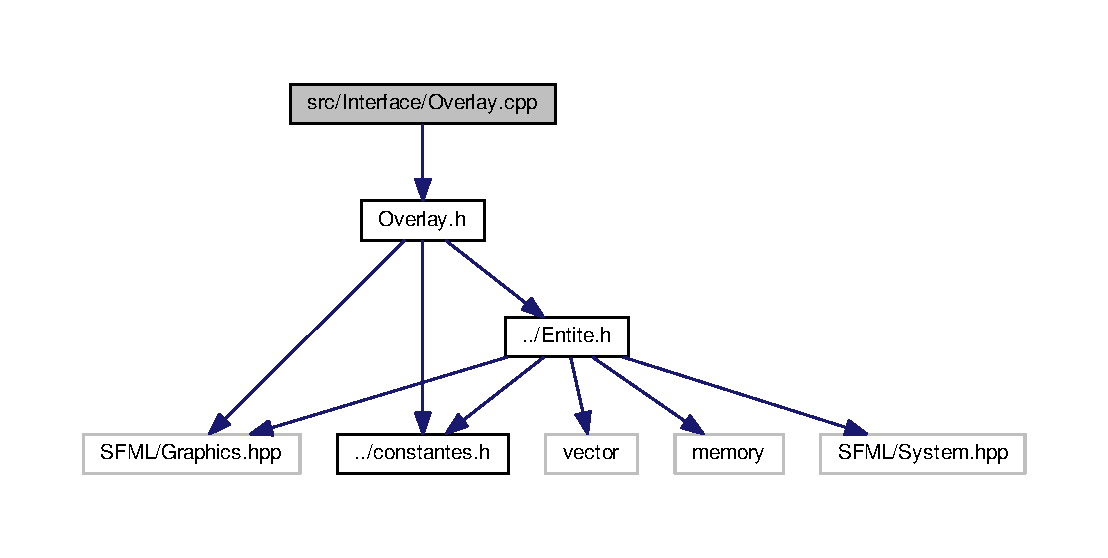
\includegraphics[width=350pt]{_overlay_8cpp__incl}
\end{center}
\end{figure}

\hypertarget{_overlay_8h}{}\section{Référence du fichier src/\+Interface/\+Overlay.h}
\label{_overlay_8h}\index{src/\+Interface/\+Overlay.\+h@{src/\+Interface/\+Overlay.\+h}}
{\ttfamily \#include \char`\"{}S\+F\+M\+L/\+Graphics.\+hpp\char`\"{}}\newline
{\ttfamily \#include \char`\"{}../constantes.\+h\char`\"{}}\newline
{\ttfamily \#include \char`\"{}../\+Vaisseau/\+Vaisseau.\+h\char`\"{}}\newline
{\ttfamily \#include $<$iostream$>$}\newline
Graphe des dépendances par inclusion de Overlay.\+h\+:
% FIG 0
Ce graphe montre quels fichiers incluent directement ou indirectement ce fichier \+:
% FIG 1
\subsection*{Classes}
\begin{DoxyCompactItemize}
\item 
class \hyperlink{class_overlay}{Overlay}
\begin{DoxyCompactList}\small\item\em Classe qui le bouton des capacité IG. \end{DoxyCompactList}\end{DoxyCompactItemize}

\hypertarget{main_8cpp}{}\section{Référence du fichier src/main.cpp}
\label{main_8cpp}\index{src/main.\+cpp@{src/main.\+cpp}}
{\ttfamily \#include $<$S\+F\+M\+L/\+Graphics.\+hpp$>$}\newline
{\ttfamily \#include $<$cmath$>$}\newline
{\ttfamily \#include $<$ctime$>$}\newline
{\ttfamily \#include $<$iostream$>$}\newline
{\ttfamily \#include \char`\"{}constantes.\+h\char`\"{}}\newline
{\ttfamily \#include \char`\"{}Entite.\+h\char`\"{}}\newline
{\ttfamily \#include \char`\"{}Collision.\+h\char`\"{}}\newline
{\ttfamily \#include \char`\"{}Partie.\+h\char`\"{}}\newline
{\ttfamily \#include \char`\"{}Input.\+h\char`\"{}}\newline
Graphe des dépendances par inclusion de main.\+cpp\+:
\nopagebreak
\begin{figure}[H]
\begin{center}
\leavevmode
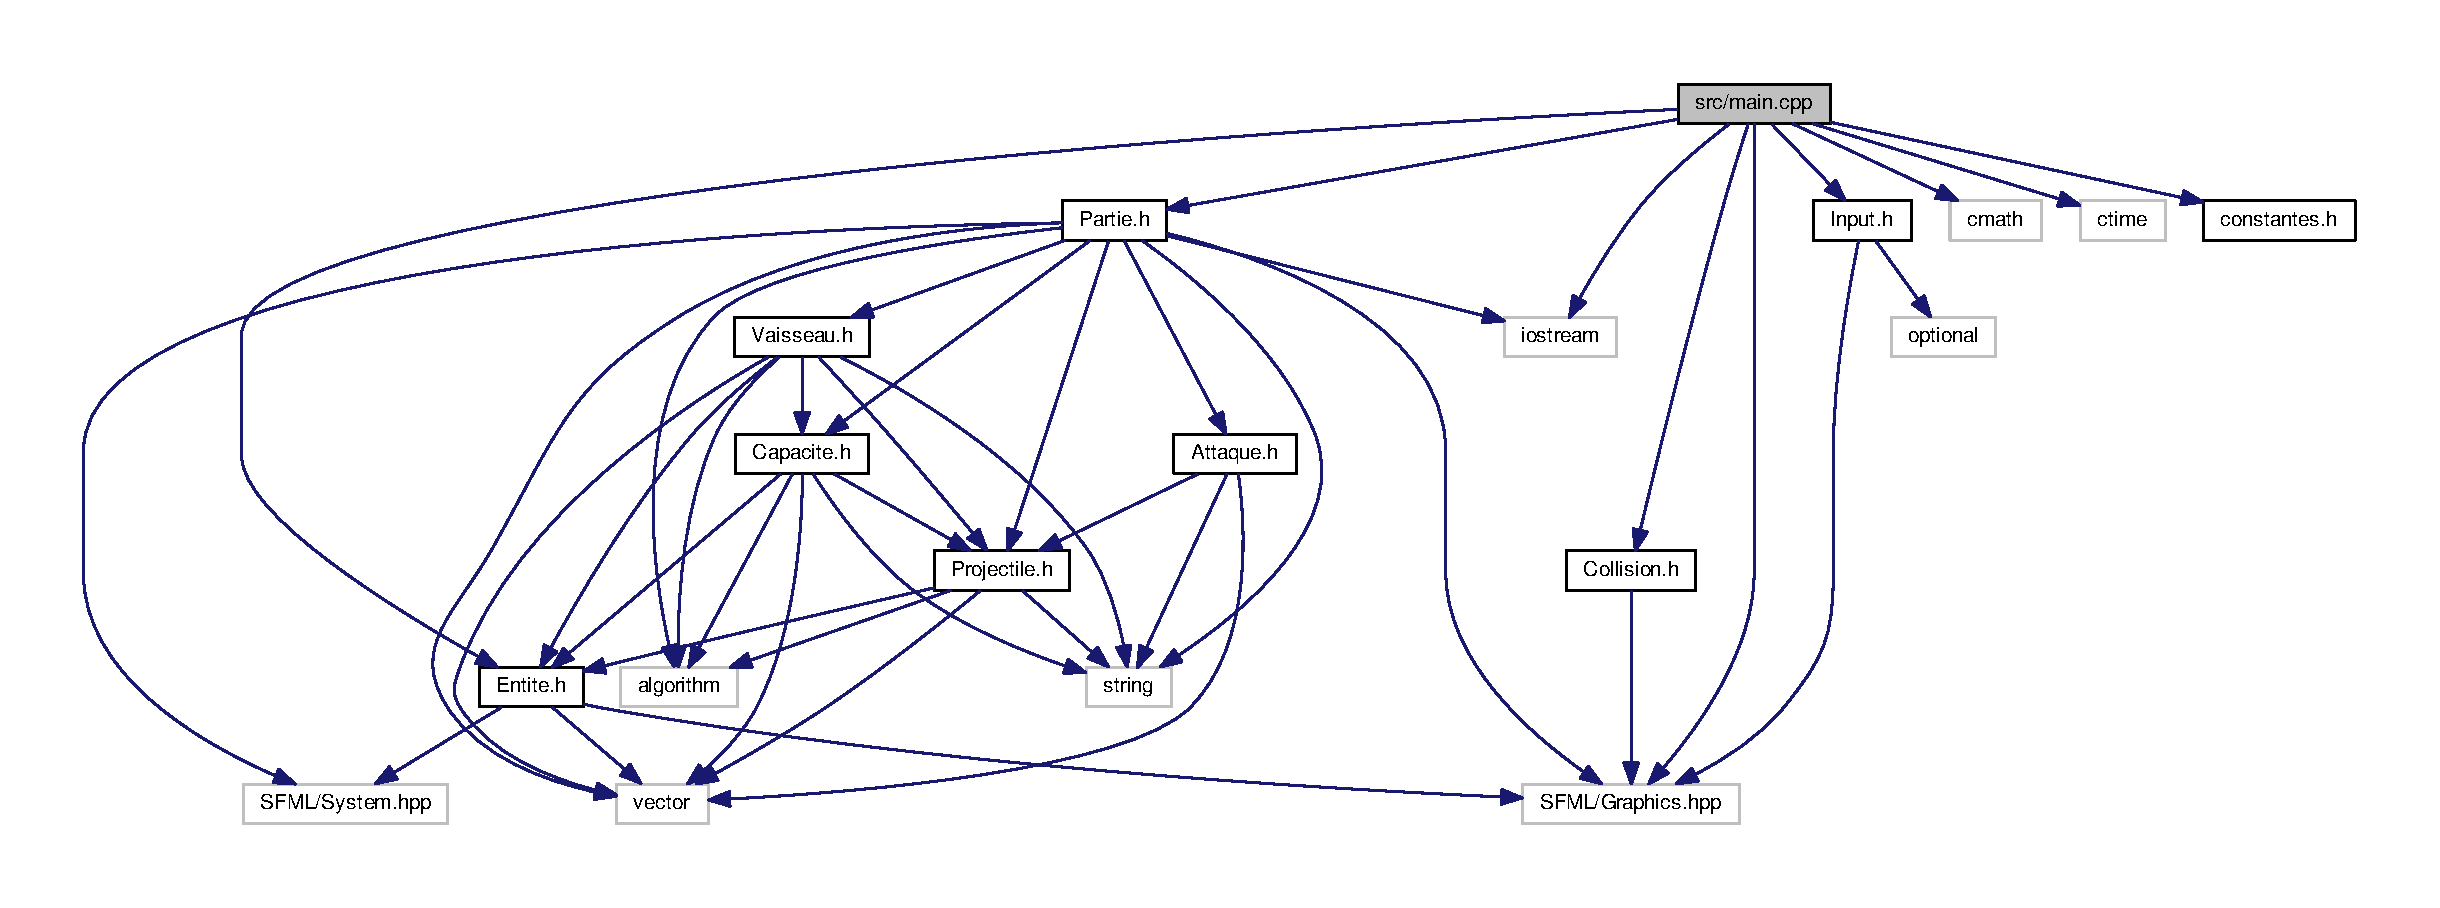
\includegraphics[width=350pt]{main_8cpp__incl}
\end{center}
\end{figure}
\subsection*{Fonctions}
\begin{DoxyCompactItemize}
\item 
int \hyperlink{main_8cpp_ae66f6b31b5ad750f1fe042a706a4e3d4}{main} ()
\end{DoxyCompactItemize}


\subsection{Documentation des fonctions}
\mbox{\Hypertarget{main_8cpp_ae66f6b31b5ad750f1fe042a706a4e3d4}\label{main_8cpp_ae66f6b31b5ad750f1fe042a706a4e3d4}} 
\index{main.\+cpp@{main.\+cpp}!main@{main}}
\index{main@{main}!main.\+cpp@{main.\+cpp}}
\subsubsection{\texorpdfstring{main()}{main()}}
{\footnotesize\ttfamily int main (\begin{DoxyParamCaption}{ }\end{DoxyParamCaption})}

$<$attention très bordélique 
\hypertarget{_partie_8cpp}{}\section{Référence du fichier src/\+Partie.cpp}
\label{_partie_8cpp}\index{src/\+Partie.\+cpp@{src/\+Partie.\+cpp}}
{\ttfamily \#include \char`\"{}Partie.\+h\char`\"{}}\newline
{\ttfamily \#include \char`\"{}Projectiles/\+\_\+projectiles.\+h\char`\"{}}\newline
{\ttfamily \#include \char`\"{}Capacites/\+\_\+\+Capacites.\+h\char`\"{}}\newline
{\ttfamily \#include \char`\"{}Vaisseau/\+\_\+vaisseaux.\+h\char`\"{}}\newline
{\ttfamily \#include \char`\"{}Interface/bindings.\+h\char`\"{}}\newline
{\ttfamily \#include \char`\"{}vague.\+h\char`\"{}}\newline
Graphe des dépendances par inclusion de Partie.\+cpp\+:\nopagebreak
\begin{figure}[H]
\begin{center}
\leavevmode
\includegraphics[width=350pt]{_partie_8cpp__incl}
\end{center}
\end{figure}

\hypertarget{_partie_8h}{}\section{src/\+Menu/\+Partie.h File Reference}
\label{_partie_8h}\index{src/\+Menu/\+Partie.\+h@{src/\+Menu/\+Partie.\+h}}
{\ttfamily \#include $<$vector$>$}\newline
{\ttfamily \#include $<$string$>$}\newline
{\ttfamily \#include $<$algorithm$>$}\newline
{\ttfamily \#include $<$iostream$>$}\newline
{\ttfamily \#include $<$memory$>$}\newline
{\ttfamily \#include $<$S\+F\+M\+L/\+Graphics.\+hpp$>$}\newline
{\ttfamily \#include $<$S\+F\+M\+L/\+System.\+hpp$>$}\newline
{\ttfamily \#include \char`\"{}../\+Capacites/\+Capacite.\+h\char`\"{}}\newline
{\ttfamily \#include \char`\"{}../\+Projectiles/\+Projectile.\+h\char`\"{}}\newline
{\ttfamily \#include \char`\"{}../\+Vaisseau/\+Vaisseau.\+h\char`\"{}}\newline
{\ttfamily \#include \char`\"{}../\+Interface/\+Input.\+h\char`\"{}}\newline
{\ttfamily \#include \char`\"{}../\+Interface/\+Overlay.\+h\char`\"{}}\newline
{\ttfamily \#include \char`\"{}../\+Pattern/\+Vague.\+h\char`\"{}}\newline
{\ttfamily \#include \char`\"{}../def\+\_\+type.\+h\char`\"{}}\newline
{\ttfamily \#include \char`\"{}Ecran.\+h\char`\"{}}\newline
\subsection*{Classes}
\begin{DoxyCompactItemize}
\item 
class \mbox{\hyperlink{class_partie}{Partie}}
\begin{DoxyCompactList}\small\item\em Description brève. \end{DoxyCompactList}\end{DoxyCompactItemize}

\hypertarget{_pattern_8cpp}{}\section{Référence du fichier src/\+Pattern/\+Pattern.cpp}
\label{_pattern_8cpp}\index{src/\+Pattern/\+Pattern.\+cpp@{src/\+Pattern/\+Pattern.\+cpp}}
{\ttfamily \#include \char`\"{}Pattern.\+h\char`\"{}}\newline
Graphe des dépendances par inclusion de Pattern.\+cpp\+:
% FIG 0

\hypertarget{_pattern_8h}{}\section{src/\+Pattern/\+Pattern.h File Reference}
\label{_pattern_8h}\index{src/\+Pattern/\+Pattern.\+h@{src/\+Pattern/\+Pattern.\+h}}
{\ttfamily \#include \char`\"{}Vague.\+h\char`\"{}}\newline
{\ttfamily \#include \char`\"{}../\+Menu/\+Partie.\+h\char`\"{}}\newline
\subsection*{Classes}
\begin{DoxyCompactItemize}
\item 
class \mbox{\hyperlink{class_pattern}{Pattern}}
\end{DoxyCompactItemize}

\hypertarget{_vague_8cpp}{}\section{Référence du fichier src/\+Pattern/\+Vague.cpp}
\label{_vague_8cpp}\index{src/\+Pattern/\+Vague.\+cpp@{src/\+Pattern/\+Vague.\+cpp}}
{\ttfamily \#include \char`\"{}Vague.\+h\char`\"{}}\newline
Graphe des dépendances par inclusion de Vague.\+cpp\+:
% FIG 0

\hypertarget{_vague_8h}{}\section{Référence du fichier src/\+Pattern/\+Vague.h}
\label{_vague_8h}\index{src/\+Pattern/\+Vague.\+h@{src/\+Pattern/\+Vague.\+h}}
{\ttfamily \#include $<$vector$>$}\newline
{\ttfamily \#include $<$S\+F\+M\+L/\+Graphics.\+hpp$>$}\newline
{\ttfamily \#include \char`\"{}../\+Vaisseau/\+\_\+vaisseaux.\+h\char`\"{}}\newline
Graphe des dépendances par inclusion de Vague.\+h\+:
% FIG 0
Ce graphe montre quels fichiers incluent directement ou indirectement ce fichier \+:
% FIG 1
\subsection*{Classes}
\begin{DoxyCompactItemize}
\item 
struct \hyperlink{struct_element_vague}{Element\+Vague}
\item 
class \hyperlink{class_vague}{Vague}
\begin{DoxyCompactList}\small\item\em Classe qui décrit les vagues d\textquotesingle{}ennemis. \end{DoxyCompactList}\end{DoxyCompactItemize}

\hypertarget{__projectiles_8h}{}\section{Référence du fichier src/\+Projectiles/\+\_\+projectiles.h}
\label{__projectiles_8h}\index{src/\+Projectiles/\+\_\+projectiles.\+h@{src/\+Projectiles/\+\_\+projectiles.\+h}}
{\ttfamily \#include \char`\"{}Proj\+Test.\+h\char`\"{}}\newline
{\ttfamily \#include \char`\"{}Proj\+Piou.\+h\char`\"{}}\newline
{\ttfamily \#include \char`\"{}Proj\+Missile.\+h\char`\"{}}\newline
Graphe des dépendances par inclusion de \+\_\+projectiles.\+h\+:\nopagebreak
\begin{figure}[H]
\begin{center}
\leavevmode
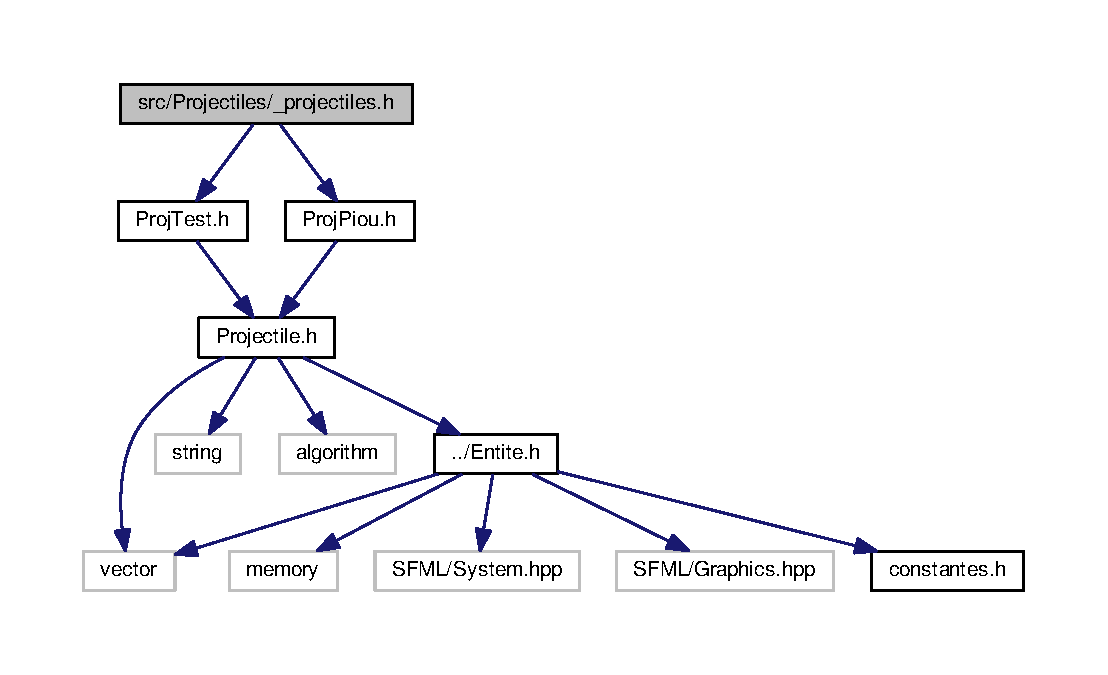
\includegraphics[width=350pt]{__projectiles_8h__incl}
\end{center}
\end{figure}
Ce graphe montre quels fichiers incluent directement ou indirectement ce fichier \+:\nopagebreak
\begin{figure}[H]
\begin{center}
\leavevmode
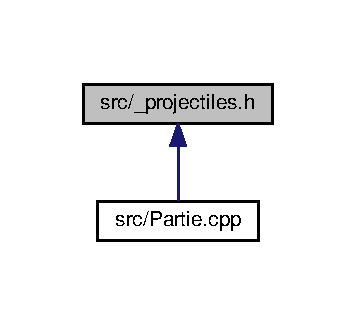
\includegraphics[width=248pt]{__projectiles_8h__dep__incl}
\end{center}
\end{figure}

\hypertarget{_proj_bismillah_8cpp}{}\section{src/\+Projectiles/\+Proj\+Bismillah.cpp File Reference}
\label{_proj_bismillah_8cpp}\index{src/\+Projectiles/\+Proj\+Bismillah.\+cpp@{src/\+Projectiles/\+Proj\+Bismillah.\+cpp}}
{\ttfamily \#include \char`\"{}Proj\+Bismillah.\+h\char`\"{}}\newline
{\ttfamily \#include $<$cmath$>$}\newline

\hypertarget{_proj_bismillah_8h}{}\section{Référence du fichier src/\+Projectiles/\+Proj\+Bismillah.h}
\label{_proj_bismillah_8h}\index{src/\+Projectiles/\+Proj\+Bismillah.\+h@{src/\+Projectiles/\+Proj\+Bismillah.\+h}}
{\ttfamily \#include \char`\"{}Projectile.\+h\char`\"{}}\newline
Graphe des dépendances par inclusion de Proj\+Bismillah.\+h\+:
% FIG 0
Ce graphe montre quels fichiers incluent directement ou indirectement ce fichier \+:
% FIG 1
\subsection*{Classes}
\begin{DoxyCompactItemize}
\item 
class \hyperlink{class_proj_bismillah}{Proj\+Bismillah}
\end{DoxyCompactItemize}

\hypertarget{_proj_boing_8cpp}{}\section{src/\+Projectiles/\+Proj\+Boing.cpp File Reference}
\label{_proj_boing_8cpp}\index{src/\+Projectiles/\+Proj\+Boing.\+cpp@{src/\+Projectiles/\+Proj\+Boing.\+cpp}}
{\ttfamily \#include \char`\"{}Proj\+Boing.\+h\char`\"{}}\newline
{\ttfamily \#include \char`\"{}../constantes.\+h\char`\"{}}\newline
{\ttfamily \#include $<$cmath$>$}\newline

\hypertarget{_proj_boing_8h}{}\section{Référence du fichier src/\+Projectiles/\+Proj\+Boing.h}
\label{_proj_boing_8h}\index{src/\+Projectiles/\+Proj\+Boing.\+h@{src/\+Projectiles/\+Proj\+Boing.\+h}}
{\ttfamily \#include \char`\"{}Projectile.\+h\char`\"{}}\newline
Graphe des dépendances par inclusion de Proj\+Boing.\+h\+:
% FIG 0
Ce graphe montre quels fichiers incluent directement ou indirectement ce fichier \+:
% FIG 1
\subsection*{Classes}
\begin{DoxyCompactItemize}
\item 
class \hyperlink{class_proj_boing}{Proj\+Boing}
\begin{DoxyCompactList}\small\item\em \hyperlink{class_projectile}{Projectile} de test. \end{DoxyCompactList}\end{DoxyCompactItemize}

\hypertarget{_proj_bouclier_rond_8cpp}{}\section{src/\+Projectiles/\+Proj\+Bouclier\+Rond.cpp File Reference}
\label{_proj_bouclier_rond_8cpp}\index{src/\+Projectiles/\+Proj\+Bouclier\+Rond.\+cpp@{src/\+Projectiles/\+Proj\+Bouclier\+Rond.\+cpp}}
{\ttfamily \#include \char`\"{}Proj\+Bouclier\+Rond.\+h\char`\"{}}\newline
{\ttfamily \#include $<$cmath$>$}\newline

\hypertarget{_proj_bouclier_rond_8h}{}\section{Référence du fichier src/\+Projectiles/\+Proj\+Bouclier\+Rond.h}
\label{_proj_bouclier_rond_8h}\index{src/\+Projectiles/\+Proj\+Bouclier\+Rond.\+h@{src/\+Projectiles/\+Proj\+Bouclier\+Rond.\+h}}
{\ttfamily \#include \char`\"{}Projectile.\+h\char`\"{}}\newline
Graphe des dépendances par inclusion de Proj\+Bouclier\+Rond.\+h\+:
% FIG 0
Ce graphe montre quels fichiers incluent directement ou indirectement ce fichier \+:
% FIG 1
\subsection*{Classes}
\begin{DoxyCompactItemize}
\item 
class \hyperlink{class_proj_bouclier_rond}{Proj\+Bouclier\+Rond}
\end{DoxyCompactItemize}

\hypertarget{_projectile_8cpp}{}\section{Référence du fichier src/\+Projectiles/\+Projectile.cpp}
\label{_projectile_8cpp}\index{src/\+Projectiles/\+Projectile.\+cpp@{src/\+Projectiles/\+Projectile.\+cpp}}
{\ttfamily \#include $<$vector$>$}\newline
{\ttfamily \#include $<$string$>$}\newline
{\ttfamily \#include $<$algorithm$>$}\newline
{\ttfamily \#include $<$S\+F\+M\+L/\+Graphics.\+hpp$>$}\newline
{\ttfamily \#include \char`\"{}../\+Capacites/\+Capacite.\+h\char`\"{}}\newline
{\ttfamily \#include \char`\"{}../\+Vaisseau/\+Vaisseau.\+h\char`\"{}}\newline
{\ttfamily \#include \char`\"{}Projectile.\+h\char`\"{}}\newline
Graphe des dépendances par inclusion de Projectile.\+cpp\+:\nopagebreak
\begin{figure}[H]
\begin{center}
\leavevmode
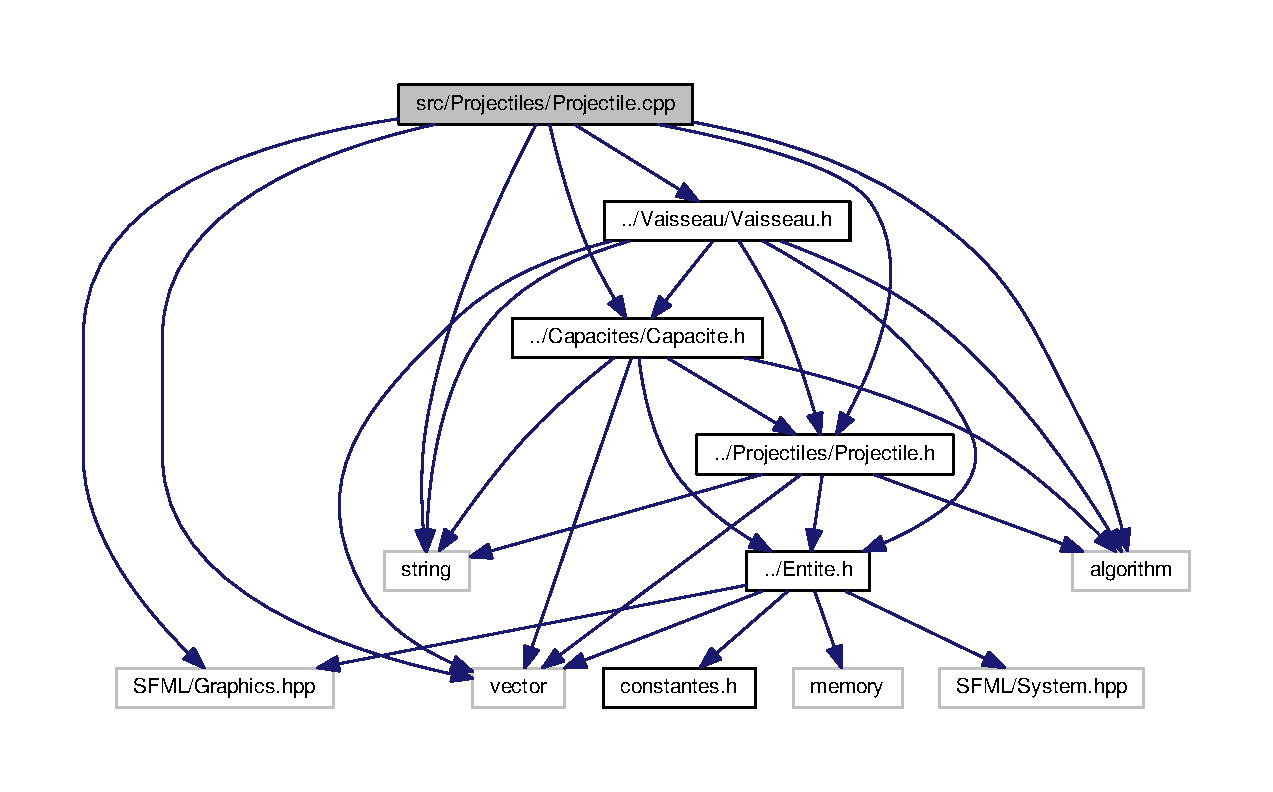
\includegraphics[width=350pt]{_projectile_8cpp__incl}
\end{center}
\end{figure}

\hypertarget{_projectile_8h}{}\section{Référence du fichier src/\+Projectiles/\+Projectile.h}
\label{_projectile_8h}\index{src/\+Projectiles/\+Projectile.\+h@{src/\+Projectiles/\+Projectile.\+h}}
{\ttfamily \#include $<$vector$>$}\newline
{\ttfamily \#include $<$string$>$}\newline
{\ttfamily \#include $<$algorithm$>$}\newline
{\ttfamily \#include \char`\"{}../\+Entite.\+h\char`\"{}}\newline
Graphe des dépendances par inclusion de Projectile.\+h\+:\nopagebreak
\begin{figure}[H]
\begin{center}
\leavevmode
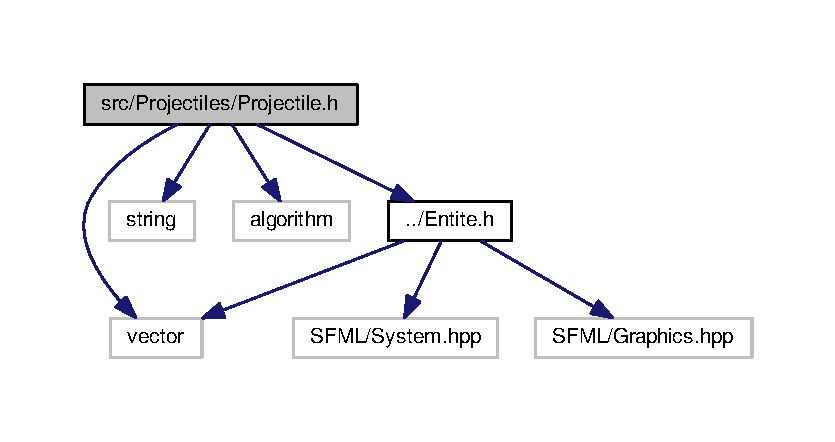
\includegraphics[width=350pt]{_projectile_8h__incl}
\end{center}
\end{figure}
Ce graphe montre quels fichiers incluent directement ou indirectement ce fichier \+:\nopagebreak
\begin{figure}[H]
\begin{center}
\leavevmode
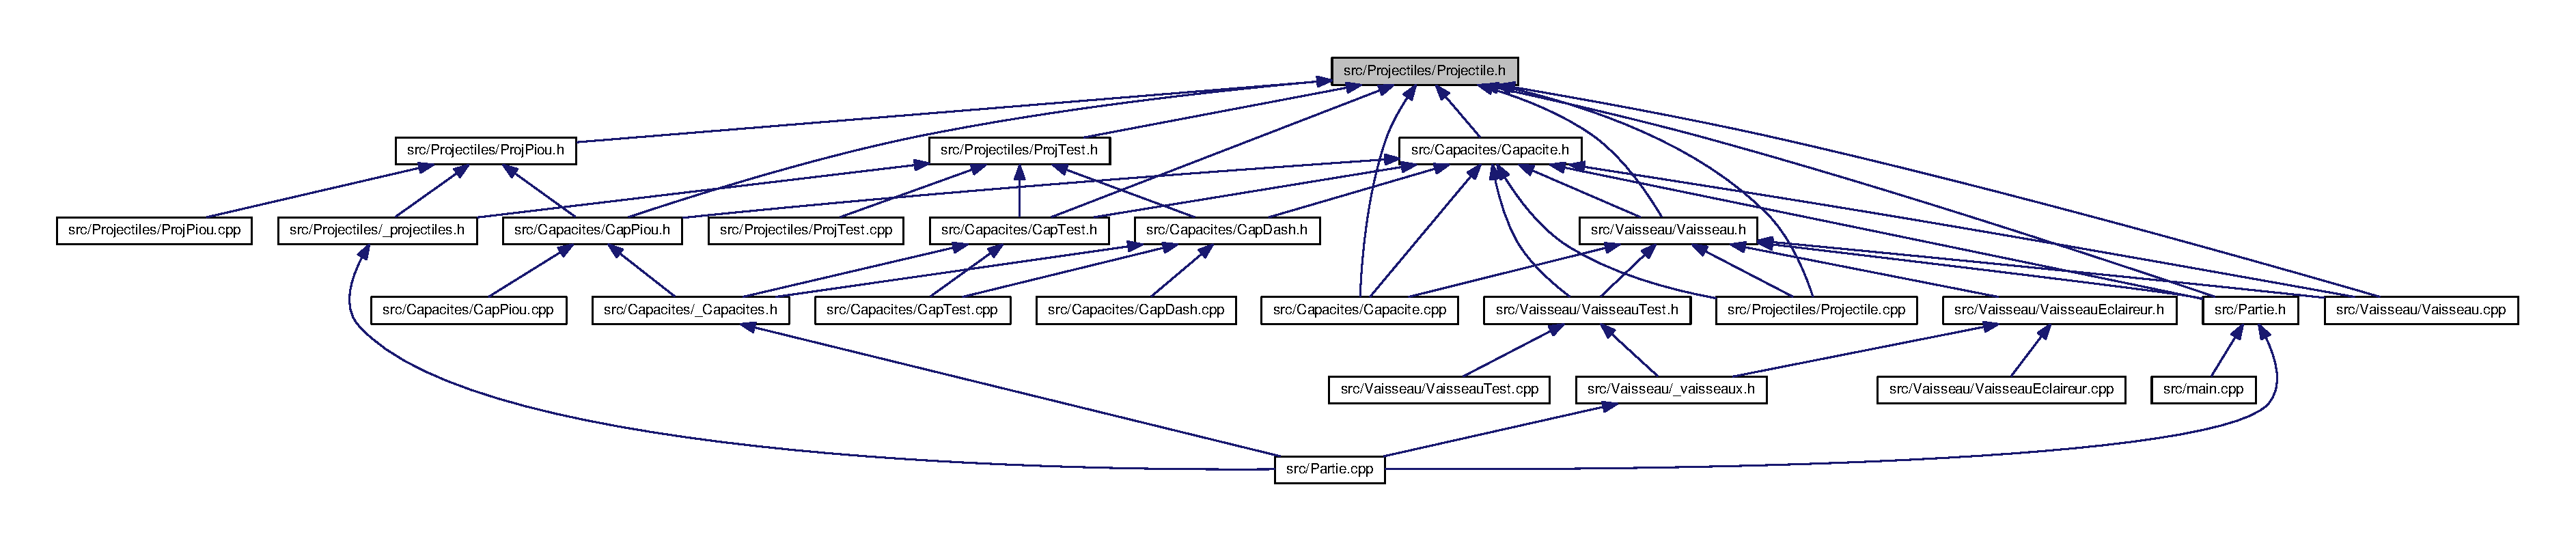
\includegraphics[width=350pt]{_projectile_8h__dep__incl}
\end{center}
\end{figure}
\subsection*{Classes}
\begin{DoxyCompactItemize}
\item 
class \hyperlink{class_projectile}{Projectile}
\begin{DoxyCompactList}\small\item\em Classe abstraite qui définit la structure générale d\textquotesingle{}un projectile, à faire hériter pour chaque projectile. \end{DoxyCompactList}\end{DoxyCompactItemize}

\hypertarget{_proj_missile_8cpp}{}\section{Référence du fichier src/\+Projectiles/\+Proj\+Missile.cpp}
\label{_proj_missile_8cpp}\index{src/\+Projectiles/\+Proj\+Missile.\+cpp@{src/\+Projectiles/\+Proj\+Missile.\+cpp}}
{\ttfamily \#include \char`\"{}Proj\+Missile.\+h\char`\"{}}\newline
{\ttfamily \#include $<$cmath$>$}\newline
Graphe des dépendances par inclusion de Proj\+Missile.\+cpp\+:
% FIG 0

\hypertarget{_proj_missile_8h}{}\section{Référence du fichier src/\+Projectiles/\+Proj\+Missile.h}
\label{_proj_missile_8h}\index{src/\+Projectiles/\+Proj\+Missile.\+h@{src/\+Projectiles/\+Proj\+Missile.\+h}}
{\ttfamily \#include \char`\"{}Projectile.\+h\char`\"{}}\newline
Graphe des dépendances par inclusion de Proj\+Missile.\+h\+:
% FIG 0
Ce graphe montre quels fichiers incluent directement ou indirectement ce fichier \+:
% FIG 1
\subsection*{Classes}
\begin{DoxyCompactItemize}
\item 
class \hyperlink{class_proj_missile}{Proj\+Missile}
\end{DoxyCompactItemize}

\hypertarget{_proj_piou_8cpp}{}\section{Référence du fichier src/\+Projectiles/\+Proj\+Piou.cpp}
\label{_proj_piou_8cpp}\index{src/\+Projectiles/\+Proj\+Piou.\+cpp@{src/\+Projectiles/\+Proj\+Piou.\+cpp}}
{\ttfamily \#include \char`\"{}Proj\+Piou.\+h\char`\"{}}\newline
{\ttfamily \#include $<$cmath$>$}\newline
Graphe des dépendances par inclusion de Proj\+Piou.\+cpp\+:\nopagebreak
\begin{figure}[H]
\begin{center}
\leavevmode
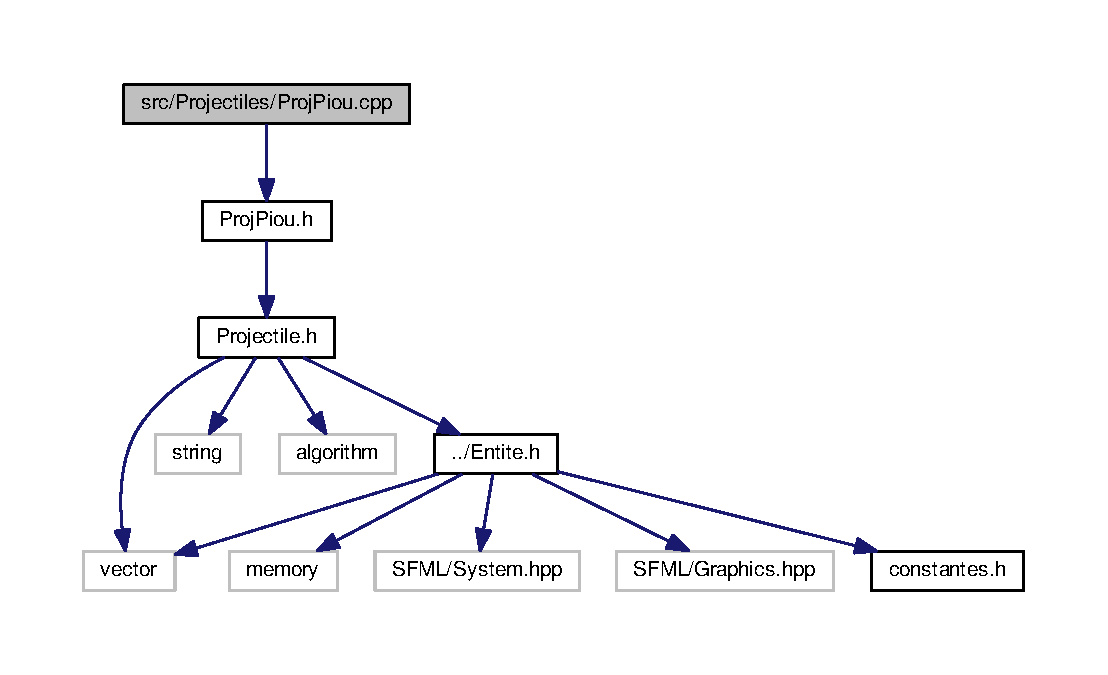
\includegraphics[width=350pt]{_proj_piou_8cpp__incl}
\end{center}
\end{figure}

\hypertarget{_proj_piou_8h}{}\section{Référence du fichier src/\+Projectiles/\+Proj\+Piou.h}
\label{_proj_piou_8h}\index{src/\+Projectiles/\+Proj\+Piou.\+h@{src/\+Projectiles/\+Proj\+Piou.\+h}}
{\ttfamily \#include \char`\"{}Projectile.\+h\char`\"{}}\newline
Graphe des dépendances par inclusion de Proj\+Piou.\+h\+:
\nopagebreak
\begin{figure}[H]
\begin{center}
\leavevmode
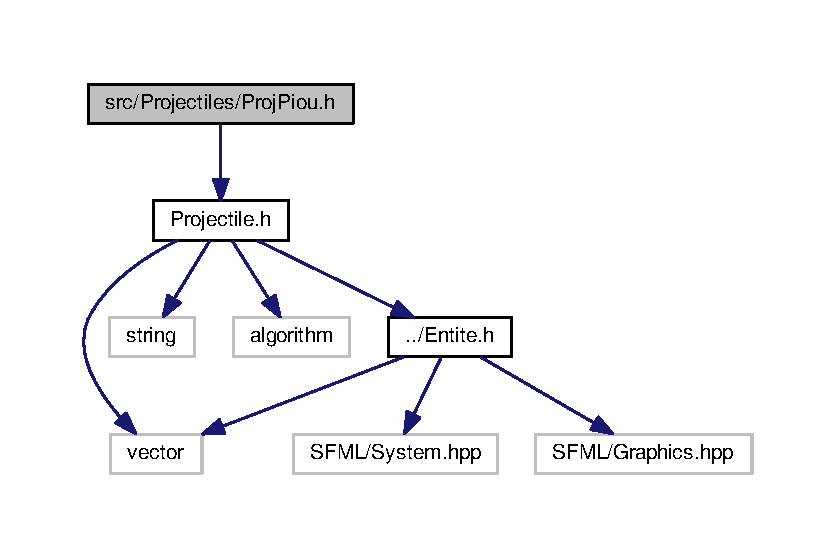
\includegraphics[width=350pt]{_proj_piou_8h__incl}
\end{center}
\end{figure}
Ce graphe montre quels fichiers incluent directement ou indirectement ce fichier \+:
\nopagebreak
\begin{figure}[H]
\begin{center}
\leavevmode
\includegraphics[width=350pt]{_proj_piou_8h__dep__incl}
\end{center}
\end{figure}
\subsection*{Classes}
\begin{DoxyCompactItemize}
\item 
class \hyperlink{class_proj_piou}{Proj\+Piou}
\end{DoxyCompactItemize}

\hypertarget{_collision_8cpp}{}\section{Référence du fichier src/\+Utilitaires/\+Collision.cpp}
\label{_collision_8cpp}\index{src/\+Utilitaires/\+Collision.\+cpp@{src/\+Utilitaires/\+Collision.\+cpp}}
{\ttfamily \#include \char`\"{}Collision.\+h\char`\"{}}\newline
{\ttfamily \#include $<$cmath$>$}\newline
Graphe des dépendances par inclusion de Collision.\+cpp\+:\nopagebreak
\begin{figure}[H]
\begin{center}
\leavevmode
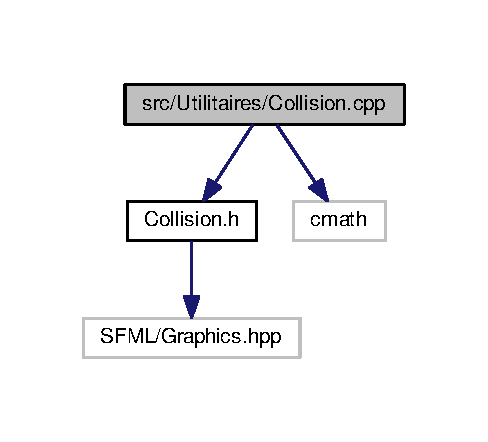
\includegraphics[width=234pt]{_collision_8cpp__incl}
\end{center}
\end{figure}
\subsection*{Fonctions}
\begin{DoxyCompactItemize}
\item 
sf\+::\+Vector2f \hyperlink{_collision_8cpp_a19be16a0d78cc53699ec1f6cc1247f0a}{centre\+\_\+transforme} (const sf\+::\+Circle\+Shape \&c)
\item 
sf\+::\+Vector2f \hyperlink{_collision_8cpp_aaf8f0e4613fb5a09397a7825b1ff4909}{point\+\_\+transforme} (const sf\+::\+Shape \&s, size\+\_\+t index)
\item 
bool \hyperlink{_collision_8cpp_a55cd5d990d317edd263c1d3bcd0b5a05}{is\+\_\+point\+\_\+in} (const sf\+::\+Vector2f \&C, const sf\+::\+Shape \&s)
\item 
bool \hyperlink{_collision_8cpp_a9037d2ebead3fc780ff50019012ac010}{collision} (const sf\+::\+Shape \&s1, const sf\+::\+Shape \&s2)
\item 
bool \hyperlink{_collision_8cpp_a4a4d2e91bbfd88f8aaaeb1572140a024}{collision\+\_\+impl} (const sf\+::\+Circle\+Shape \&c1, const sf\+::\+Circle\+Shape \&c2)
\item 
bool \hyperlink{_collision_8cpp_a598969c4bf7355123d972d3cf69eafd5}{collision\+\_\+impl} (const sf\+::\+Circle\+Shape \&c, const sf\+::\+Shape \&co)
\item 
bool \hyperlink{_collision_8cpp_adcae147b4b5b0ca770cfbc5b1c65873d}{collision\+\_\+impl} (const sf\+::\+Shape \&co, const sf\+::\+Circle\+Shape \&c)
\item 
bool \hyperlink{_collision_8cpp_ad5b149f81d5c820b0f81e5ca66385dee}{collision\+\_\+impl} (const sf\+::\+Shape \&s1, const sf\+::\+Shape \&s2)
\end{DoxyCompactItemize}
\subsection*{Variables}
\begin{DoxyCompactItemize}
\item 
const double \hyperlink{_collision_8cpp_a952eac791b596a61bba0a133a3bb439f}{PI} = acos(-\/1)
\end{DoxyCompactItemize}


\subsection{Documentation des fonctions}
\mbox{\Hypertarget{_collision_8cpp_a19be16a0d78cc53699ec1f6cc1247f0a}\label{_collision_8cpp_a19be16a0d78cc53699ec1f6cc1247f0a}} 
\index{Collision.\+cpp@{Collision.\+cpp}!centre\+\_\+transforme@{centre\+\_\+transforme}}
\index{centre\+\_\+transforme@{centre\+\_\+transforme}!Collision.\+cpp@{Collision.\+cpp}}
\subsubsection{\texorpdfstring{centre\+\_\+transforme()}{centre\_transforme()}}
{\footnotesize\ttfamily sf\+::\+Vector2f centre\+\_\+transforme (\begin{DoxyParamCaption}\item[{const sf\+::\+Circle\+Shape \&}]{c }\end{DoxyParamCaption})}

\mbox{\Hypertarget{_collision_8cpp_a9037d2ebead3fc780ff50019012ac010}\label{_collision_8cpp_a9037d2ebead3fc780ff50019012ac010}} 
\index{Collision.\+cpp@{Collision.\+cpp}!collision@{collision}}
\index{collision@{collision}!Collision.\+cpp@{Collision.\+cpp}}
\subsubsection{\texorpdfstring{collision()}{collision()}}
{\footnotesize\ttfamily bool collision (\begin{DoxyParamCaption}\item[{const sf\+::\+Shape \&}]{s1,  }\item[{const sf\+::\+Shape \&}]{s2 }\end{DoxyParamCaption})}

\mbox{\Hypertarget{_collision_8cpp_a4a4d2e91bbfd88f8aaaeb1572140a024}\label{_collision_8cpp_a4a4d2e91bbfd88f8aaaeb1572140a024}} 
\index{Collision.\+cpp@{Collision.\+cpp}!collision\+\_\+impl@{collision\+\_\+impl}}
\index{collision\+\_\+impl@{collision\+\_\+impl}!Collision.\+cpp@{Collision.\+cpp}}
\subsubsection{\texorpdfstring{collision\+\_\+impl()}{collision\_impl()}\hspace{0.1cm}{\footnotesize\ttfamily [1/4]}}
{\footnotesize\ttfamily bool collision\+\_\+impl (\begin{DoxyParamCaption}\item[{const sf\+::\+Circle\+Shape \&}]{c1,  }\item[{const sf\+::\+Circle\+Shape \&}]{c2 }\end{DoxyParamCaption})}

\mbox{\Hypertarget{_collision_8cpp_a598969c4bf7355123d972d3cf69eafd5}\label{_collision_8cpp_a598969c4bf7355123d972d3cf69eafd5}} 
\index{Collision.\+cpp@{Collision.\+cpp}!collision\+\_\+impl@{collision\+\_\+impl}}
\index{collision\+\_\+impl@{collision\+\_\+impl}!Collision.\+cpp@{Collision.\+cpp}}
\subsubsection{\texorpdfstring{collision\+\_\+impl()}{collision\_impl()}\hspace{0.1cm}{\footnotesize\ttfamily [2/4]}}
{\footnotesize\ttfamily bool collision\+\_\+impl (\begin{DoxyParamCaption}\item[{const sf\+::\+Circle\+Shape \&}]{c,  }\item[{const sf\+::\+Shape \&}]{co }\end{DoxyParamCaption})}

\mbox{\Hypertarget{_collision_8cpp_adcae147b4b5b0ca770cfbc5b1c65873d}\label{_collision_8cpp_adcae147b4b5b0ca770cfbc5b1c65873d}} 
\index{Collision.\+cpp@{Collision.\+cpp}!collision\+\_\+impl@{collision\+\_\+impl}}
\index{collision\+\_\+impl@{collision\+\_\+impl}!Collision.\+cpp@{Collision.\+cpp}}
\subsubsection{\texorpdfstring{collision\+\_\+impl()}{collision\_impl()}\hspace{0.1cm}{\footnotesize\ttfamily [3/4]}}
{\footnotesize\ttfamily bool collision\+\_\+impl (\begin{DoxyParamCaption}\item[{const sf\+::\+Shape \&}]{co,  }\item[{const sf\+::\+Circle\+Shape \&}]{c }\end{DoxyParamCaption})}

\mbox{\Hypertarget{_collision_8cpp_ad5b149f81d5c820b0f81e5ca66385dee}\label{_collision_8cpp_ad5b149f81d5c820b0f81e5ca66385dee}} 
\index{Collision.\+cpp@{Collision.\+cpp}!collision\+\_\+impl@{collision\+\_\+impl}}
\index{collision\+\_\+impl@{collision\+\_\+impl}!Collision.\+cpp@{Collision.\+cpp}}
\subsubsection{\texorpdfstring{collision\+\_\+impl()}{collision\_impl()}\hspace{0.1cm}{\footnotesize\ttfamily [4/4]}}
{\footnotesize\ttfamily bool collision\+\_\+impl (\begin{DoxyParamCaption}\item[{const sf\+::\+Shape \&}]{s1,  }\item[{const sf\+::\+Shape \&}]{s2 }\end{DoxyParamCaption})}

\mbox{\Hypertarget{_collision_8cpp_a55cd5d990d317edd263c1d3bcd0b5a05}\label{_collision_8cpp_a55cd5d990d317edd263c1d3bcd0b5a05}} 
\index{Collision.\+cpp@{Collision.\+cpp}!is\+\_\+point\+\_\+in@{is\+\_\+point\+\_\+in}}
\index{is\+\_\+point\+\_\+in@{is\+\_\+point\+\_\+in}!Collision.\+cpp@{Collision.\+cpp}}
\subsubsection{\texorpdfstring{is\+\_\+point\+\_\+in()}{is\_point\_in()}}
{\footnotesize\ttfamily bool is\+\_\+point\+\_\+in (\begin{DoxyParamCaption}\item[{const sf\+::\+Vector2f \&}]{C,  }\item[{const sf\+::\+Shape \&}]{s }\end{DoxyParamCaption})}

\mbox{\Hypertarget{_collision_8cpp_aaf8f0e4613fb5a09397a7825b1ff4909}\label{_collision_8cpp_aaf8f0e4613fb5a09397a7825b1ff4909}} 
\index{Collision.\+cpp@{Collision.\+cpp}!point\+\_\+transforme@{point\+\_\+transforme}}
\index{point\+\_\+transforme@{point\+\_\+transforme}!Collision.\+cpp@{Collision.\+cpp}}
\subsubsection{\texorpdfstring{point\+\_\+transforme()}{point\_transforme()}}
{\footnotesize\ttfamily sf\+::\+Vector2f point\+\_\+transforme (\begin{DoxyParamCaption}\item[{const sf\+::\+Shape \&}]{s,  }\item[{size\+\_\+t}]{index }\end{DoxyParamCaption})}



\subsection{Documentation des variables}
\mbox{\Hypertarget{_collision_8cpp_a952eac791b596a61bba0a133a3bb439f}\label{_collision_8cpp_a952eac791b596a61bba0a133a3bb439f}} 
\index{Collision.\+cpp@{Collision.\+cpp}!PI@{PI}}
\index{PI@{PI}!Collision.\+cpp@{Collision.\+cpp}}
\subsubsection{\texorpdfstring{PI}{PI}}
{\footnotesize\ttfamily const double PI = acos(-\/1)}


\hypertarget{_collision_8h}{}\section{src/\+Utilitaires/\+Collision.h File Reference}
\label{_collision_8h}\index{src/\+Utilitaires/\+Collision.\+h@{src/\+Utilitaires/\+Collision.\+h}}
{\ttfamily \#include $<$S\+F\+M\+L/\+Graphics.\+hpp$>$}\newline
\subsection*{Functions}
\begin{DoxyCompactItemize}
\item 
bool \mbox{\hyperlink{_collision_8h_a9037d2ebead3fc780ff50019012ac010}{collision}} (const sf\+::\+Shape \&s1, const sf\+::\+Shape \&s2)
\item 
bool \mbox{\hyperlink{_collision_8h_ad5b149f81d5c820b0f81e5ca66385dee}{collision\+\_\+impl}} (const sf\+::\+Shape \&s1, const sf\+::\+Shape \&s2)
\item 
bool \mbox{\hyperlink{_collision_8h_a4a4d2e91bbfd88f8aaaeb1572140a024}{collision\+\_\+impl}} (const sf\+::\+Circle\+Shape \&c1, const sf\+::\+Circle\+Shape \&c2)
\item 
bool \mbox{\hyperlink{_collision_8h_a598969c4bf7355123d972d3cf69eafd5}{collision\+\_\+impl}} (const sf\+::\+Circle\+Shape \&c, const sf\+::\+Shape \&co)
\item 
bool \mbox{\hyperlink{_collision_8h_adcae147b4b5b0ca770cfbc5b1c65873d}{collision\+\_\+impl}} (const sf\+::\+Shape \&co, const sf\+::\+Circle\+Shape \&c)
\end{DoxyCompactItemize}


\subsection{Function Documentation}
\mbox{\Hypertarget{_collision_8h_a9037d2ebead3fc780ff50019012ac010}\label{_collision_8h_a9037d2ebead3fc780ff50019012ac010}} 
\index{Collision.\+h@{Collision.\+h}!collision@{collision}}
\index{collision@{collision}!Collision.\+h@{Collision.\+h}}
\subsubsection{\texorpdfstring{collision()}{collision()}}
{\footnotesize\ttfamily bool collision (\begin{DoxyParamCaption}\item[{const sf\+::\+Shape \&}]{s1,  }\item[{const sf\+::\+Shape \&}]{s2 }\end{DoxyParamCaption})}

\mbox{\Hypertarget{_collision_8h_ad5b149f81d5c820b0f81e5ca66385dee}\label{_collision_8h_ad5b149f81d5c820b0f81e5ca66385dee}} 
\index{Collision.\+h@{Collision.\+h}!collision\+\_\+impl@{collision\+\_\+impl}}
\index{collision\+\_\+impl@{collision\+\_\+impl}!Collision.\+h@{Collision.\+h}}
\subsubsection{\texorpdfstring{collision\+\_\+impl()}{collision\_impl()}\hspace{0.1cm}{\footnotesize\ttfamily [1/4]}}
{\footnotesize\ttfamily bool collision\+\_\+impl (\begin{DoxyParamCaption}\item[{const sf\+::\+Shape \&}]{s1,  }\item[{const sf\+::\+Shape \&}]{s2 }\end{DoxyParamCaption})}

\mbox{\Hypertarget{_collision_8h_a4a4d2e91bbfd88f8aaaeb1572140a024}\label{_collision_8h_a4a4d2e91bbfd88f8aaaeb1572140a024}} 
\index{Collision.\+h@{Collision.\+h}!collision\+\_\+impl@{collision\+\_\+impl}}
\index{collision\+\_\+impl@{collision\+\_\+impl}!Collision.\+h@{Collision.\+h}}
\subsubsection{\texorpdfstring{collision\+\_\+impl()}{collision\_impl()}\hspace{0.1cm}{\footnotesize\ttfamily [2/4]}}
{\footnotesize\ttfamily bool collision\+\_\+impl (\begin{DoxyParamCaption}\item[{const sf\+::\+Circle\+Shape \&}]{c1,  }\item[{const sf\+::\+Circle\+Shape \&}]{c2 }\end{DoxyParamCaption})}

\mbox{\Hypertarget{_collision_8h_a598969c4bf7355123d972d3cf69eafd5}\label{_collision_8h_a598969c4bf7355123d972d3cf69eafd5}} 
\index{Collision.\+h@{Collision.\+h}!collision\+\_\+impl@{collision\+\_\+impl}}
\index{collision\+\_\+impl@{collision\+\_\+impl}!Collision.\+h@{Collision.\+h}}
\subsubsection{\texorpdfstring{collision\+\_\+impl()}{collision\_impl()}\hspace{0.1cm}{\footnotesize\ttfamily [3/4]}}
{\footnotesize\ttfamily bool collision\+\_\+impl (\begin{DoxyParamCaption}\item[{const sf\+::\+Circle\+Shape \&}]{c,  }\item[{const sf\+::\+Shape \&}]{co }\end{DoxyParamCaption})}

\mbox{\Hypertarget{_collision_8h_adcae147b4b5b0ca770cfbc5b1c65873d}\label{_collision_8h_adcae147b4b5b0ca770cfbc5b1c65873d}} 
\index{Collision.\+h@{Collision.\+h}!collision\+\_\+impl@{collision\+\_\+impl}}
\index{collision\+\_\+impl@{collision\+\_\+impl}!Collision.\+h@{Collision.\+h}}
\subsubsection{\texorpdfstring{collision\+\_\+impl()}{collision\_impl()}\hspace{0.1cm}{\footnotesize\ttfamily [4/4]}}
{\footnotesize\ttfamily bool collision\+\_\+impl (\begin{DoxyParamCaption}\item[{const sf\+::\+Shape \&}]{co,  }\item[{const sf\+::\+Circle\+Shape \&}]{c }\end{DoxyParamCaption})}


\hypertarget{_divers_8h}{}\section{src/\+Utilitaires/\+Divers.h File Reference}
\label{_divers_8h}\index{src/\+Utilitaires/\+Divers.\+h@{src/\+Utilitaires/\+Divers.\+h}}
{\ttfamily \#include \char`\"{}../\+Entite.\+h\char`\"{}}\newline
{\ttfamily \#include $<$S\+F\+M\+L/\+Graphics.\+hpp$>$}\newline
{\ttfamily \#include $<$string$>$}\newline
{\ttfamily \#include $<$memory$>$}\newline
\subsection*{Functions}
\begin{DoxyCompactItemize}
\item 
{\footnotesize template$<$typename T , typename U $>$ }\\bool \mbox{\hyperlink{_divers_8h_a3b8884aabd0ad28b2d790bf0752f6984}{est}} (const T \&X)
\item 
void \mbox{\hyperlink{_divers_8h_aeabc946ae0fa583e72aff6e8b7e6cbbc}{adapt\+\_\+viewport}} (sf\+::\+Render\+Window \&window)
\item 
std\+::string \mbox{\hyperlink{_divers_8h_a9b855aac79a01bc69b093a4ee12bb688}{trim}} (std\+::string str)
\item 
std\+::pair$<$ std\+::string, std\+::string $>$ \mbox{\hyperlink{_divers_8h_a9a29f7315011778d15db9366fbcbe556}{tokenize}} (const std\+::string \&str, char sep)
\item 
double \mbox{\hyperlink{_divers_8h_afe48d80943fa9e3ea1f39998f66213a7}{rayon\+\_\+englobeur}} (const std\+::vector$<$ std\+::unique\+\_\+ptr$<$ sf\+::\+Shape $>$$>$ \&forme, sf\+::\+Vector2f origine)
\item 
void \mbox{\hyperlink{_divers_8h_afffd86758e1fafd47919e5874a1e93f6}{englobeur\+\_\+circulaire}} (\mbox{\hyperlink{class_entite}{Entite}} \&entite)
\end{DoxyCompactItemize}


\subsection{Function Documentation}
\mbox{\Hypertarget{_divers_8h_aeabc946ae0fa583e72aff6e8b7e6cbbc}\label{_divers_8h_aeabc946ae0fa583e72aff6e8b7e6cbbc}} 
\index{Divers.\+h@{Divers.\+h}!adapt\+\_\+viewport@{adapt\+\_\+viewport}}
\index{adapt\+\_\+viewport@{adapt\+\_\+viewport}!Divers.\+h@{Divers.\+h}}
\subsubsection{\texorpdfstring{adapt\+\_\+viewport()}{adapt\_viewport()}}
{\footnotesize\ttfamily void adapt\+\_\+viewport (\begin{DoxyParamCaption}\item[{sf\+::\+Render\+Window \&}]{window }\end{DoxyParamCaption})}

\mbox{\Hypertarget{_divers_8h_afffd86758e1fafd47919e5874a1e93f6}\label{_divers_8h_afffd86758e1fafd47919e5874a1e93f6}} 
\index{Divers.\+h@{Divers.\+h}!englobeur\+\_\+circulaire@{englobeur\+\_\+circulaire}}
\index{englobeur\+\_\+circulaire@{englobeur\+\_\+circulaire}!Divers.\+h@{Divers.\+h}}
\subsubsection{\texorpdfstring{englobeur\+\_\+circulaire()}{englobeur\_circulaire()}}
{\footnotesize\ttfamily void englobeur\+\_\+circulaire (\begin{DoxyParamCaption}\item[{\mbox{\hyperlink{class_entite}{Entite}} \&}]{entite }\end{DoxyParamCaption})}

\mbox{\Hypertarget{_divers_8h_a3b8884aabd0ad28b2d790bf0752f6984}\label{_divers_8h_a3b8884aabd0ad28b2d790bf0752f6984}} 
\index{Divers.\+h@{Divers.\+h}!est@{est}}
\index{est@{est}!Divers.\+h@{Divers.\+h}}
\subsubsection{\texorpdfstring{est()}{est()}}
{\footnotesize\ttfamily template$<$typename T , typename U $>$ \\
bool est (\begin{DoxyParamCaption}\item[{const T \&}]{X }\end{DoxyParamCaption})}

\mbox{\Hypertarget{_divers_8h_afe48d80943fa9e3ea1f39998f66213a7}\label{_divers_8h_afe48d80943fa9e3ea1f39998f66213a7}} 
\index{Divers.\+h@{Divers.\+h}!rayon\+\_\+englobeur@{rayon\+\_\+englobeur}}
\index{rayon\+\_\+englobeur@{rayon\+\_\+englobeur}!Divers.\+h@{Divers.\+h}}
\subsubsection{\texorpdfstring{rayon\+\_\+englobeur()}{rayon\_englobeur()}}
{\footnotesize\ttfamily double rayon\+\_\+englobeur (\begin{DoxyParamCaption}\item[{const std\+::vector$<$ std\+::unique\+\_\+ptr$<$ sf\+::\+Shape $>$$>$ \&}]{forme,  }\item[{sf\+::\+Vector2f}]{origine }\end{DoxyParamCaption})}

\mbox{\Hypertarget{_divers_8h_a9a29f7315011778d15db9366fbcbe556}\label{_divers_8h_a9a29f7315011778d15db9366fbcbe556}} 
\index{Divers.\+h@{Divers.\+h}!tokenize@{tokenize}}
\index{tokenize@{tokenize}!Divers.\+h@{Divers.\+h}}
\subsubsection{\texorpdfstring{tokenize()}{tokenize()}}
{\footnotesize\ttfamily std\+::pair$<$std\+::string, std\+::string$>$ tokenize (\begin{DoxyParamCaption}\item[{const std\+::string \&}]{str,  }\item[{char}]{sep }\end{DoxyParamCaption})}

\mbox{\Hypertarget{_divers_8h_a9b855aac79a01bc69b093a4ee12bb688}\label{_divers_8h_a9b855aac79a01bc69b093a4ee12bb688}} 
\index{Divers.\+h@{Divers.\+h}!trim@{trim}}
\index{trim@{trim}!Divers.\+h@{Divers.\+h}}
\subsubsection{\texorpdfstring{trim()}{trim()}}
{\footnotesize\ttfamily std\+::string trim (\begin{DoxyParamCaption}\item[{std\+::string}]{str }\end{DoxyParamCaption})}


\hypertarget{optional_8h}{}\section{Référence du fichier src/\+Utilitaires/optional.h}
\label{optional_8h}\index{src/\+Utilitaires/optional.\+h@{src/\+Utilitaires/optional.\+h}}
{\ttfamily \#include $<$utility$>$}\newline
{\ttfamily \#include $<$type\+\_\+traits$>$}\newline
{\ttfamily \#include $<$initializer\+\_\+list$>$}\newline
{\ttfamily \#include $<$cassert$>$}\newline
{\ttfamily \#include $<$functional$>$}\newline
{\ttfamily \#include $<$string$>$}\newline
{\ttfamily \#include $<$stdexcept$>$}\newline
Graphe des dépendances par inclusion de optional.\+h\+:
% FIG 0
Ce graphe montre quels fichiers incluent directement ou indirectement ce fichier \+:
% FIG 1
\subsection*{Classes}
\begin{DoxyCompactItemize}
\item 
struct \hyperlink{structstd_1_1experimental_1_1is__nothrow__move__constructible}{std\+::experimental\+::is\+\_\+nothrow\+\_\+move\+\_\+constructible$<$ T $>$}
\item 
struct \hyperlink{structstd_1_1experimental_1_1is__assignable}{std\+::experimental\+::is\+\_\+assignable$<$ T, U $>$}
\item 
struct \hyperlink{structstd_1_1experimental_1_1is__nothrow__move__assignable}{std\+::experimental\+::is\+\_\+nothrow\+\_\+move\+\_\+assignable$<$ T $>$}
\item 
struct \hyperlink{structstd_1_1experimental_1_1is__nothrow__move__assignable_1_1has__nothrow__move__assign}{std\+::experimental\+::is\+\_\+nothrow\+\_\+move\+\_\+assignable$<$ T $>$\+::has\+\_\+nothrow\+\_\+move\+\_\+assign$<$ X, has\+\_\+any\+\_\+move\+\_\+assign $>$}
\item 
struct \hyperlink{structstd_1_1experimental_1_1is__nothrow__move__assignable_1_1has__nothrow__move__assign_3_01_x_00_01true_01_4}{std\+::experimental\+::is\+\_\+nothrow\+\_\+move\+\_\+assignable$<$ T $>$\+::has\+\_\+nothrow\+\_\+move\+\_\+assign$<$ X, true $>$}
\item 
class \hyperlink{classstd_1_1experimental_1_1optional}{std\+::experimental\+::optional$<$ T $>$}
\item 
struct \hyperlink{structstd_1_1experimental_1_1detail___1_1has__overloaded__addressof}{std\+::experimental\+::detail\+\_\+\+::has\+\_\+overloaded\+\_\+addressof$<$ T $>$}
\item 
struct \hyperlink{structstd_1_1experimental_1_1trivial__init__t}{std\+::experimental\+::trivial\+\_\+init\+\_\+t}
\item 
struct \hyperlink{structstd_1_1experimental_1_1in__place__t}{std\+::experimental\+::in\+\_\+place\+\_\+t}
\item 
struct \hyperlink{structstd_1_1experimental_1_1nullopt__t}{std\+::experimental\+::nullopt\+\_\+t}
\item 
struct \hyperlink{structstd_1_1experimental_1_1nullopt__t_1_1init}{std\+::experimental\+::nullopt\+\_\+t\+::init}
\item 
class \hyperlink{classstd_1_1experimental_1_1bad__optional__access}{std\+::experimental\+::bad\+\_\+optional\+\_\+access}
\item 
union \hyperlink{unionstd_1_1experimental_1_1storage__t}{std\+::experimental\+::storage\+\_\+t$<$ T $>$}
\item 
union \hyperlink{unionstd_1_1experimental_1_1constexpr__storage__t}{std\+::experimental\+::constexpr\+\_\+storage\+\_\+t$<$ T $>$}
\item 
struct \hyperlink{structstd_1_1experimental_1_1optional__base}{std\+::experimental\+::optional\+\_\+base$<$ T $>$}
\item 
struct \hyperlink{structstd_1_1experimental_1_1constexpr__optional__base}{std\+::experimental\+::constexpr\+\_\+optional\+\_\+base$<$ T $>$}
\item 
class \hyperlink{classstd_1_1experimental_1_1optional}{std\+::experimental\+::optional$<$ T $>$}
\item 
class \hyperlink{classstd_1_1experimental_1_1optional_3_01_t_01_6_01_4}{std\+::experimental\+::optional$<$ T \& $>$}
\item 
class \hyperlink{classstd_1_1experimental_1_1optional_3_01_t_01_6_6_01_4}{std\+::experimental\+::optional$<$ T \&\& $>$}
\item 
struct \hyperlink{structstd_1_1hash_3_01std_1_1experimental_1_1optional_3_01_t_01_4_01_4}{std\+::hash$<$ std\+::experimental\+::optional$<$ T $>$ $>$}
\item 
struct \hyperlink{structstd_1_1hash_3_01std_1_1experimental_1_1optional_3_01_t_01_6_01_4_01_4}{std\+::hash$<$ std\+::experimental\+::optional$<$ T \& $>$ $>$}
\end{DoxyCompactItemize}
\subsection*{Espaces de nommage}
\begin{DoxyCompactItemize}
\item 
 \hyperlink{namespacestd}{std}
\item 
 \hyperlink{namespacestd_1_1experimental}{std\+::experimental}
\item 
 \hyperlink{namespacestd_1_1experimental_1_1detail__}{std\+::experimental\+::detail\+\_\+}
\end{DoxyCompactItemize}
\subsection*{Macros}
\begin{DoxyCompactItemize}
\item 
\#define \hyperlink{optional_8h_a2bc77cf029dcdedaf87668a8da6e899b}{T\+R2\+\_\+\+O\+P\+T\+I\+O\+N\+A\+L\+\_\+\+R\+E\+Q\+U\+I\+R\+ES}(...)~typename enable\+\_\+if$<$\+\_\+\+\_\+\+V\+A\+\_\+\+A\+R\+G\+S\+\_\+\+\_\+\+::value, bool$>$\+::type = false
\item 
\#define \hyperlink{optional_8h_a2fb97d4b996dbddf95c6c25b64e5abb5}{O\+P\+T\+I\+O\+N\+A\+L\+\_\+\+H\+A\+S\+\_\+\+T\+H\+I\+S\+\_\+\+R\+V\+A\+L\+U\+E\+\_\+\+R\+E\+FS}~0
\item 
\#define \hyperlink{optional_8h_af240286c9615958c84d4e886d29022e2}{O\+P\+T\+I\+O\+N\+A\+L\+\_\+\+H\+A\+S\+\_\+\+C\+O\+N\+S\+T\+E\+X\+P\+R\+\_\+\+I\+N\+I\+T\+\_\+\+L\+I\+ST}~0
\item 
\#define \hyperlink{optional_8h_a7399114ed1c146a67741cdd1f681fcb5}{O\+P\+T\+I\+O\+N\+A\+L\+\_\+\+C\+O\+N\+S\+T\+E\+X\+P\+R\+\_\+\+I\+N\+I\+T\+\_\+\+L\+I\+ST}
\item 
\#define \hyperlink{optional_8h_a6e00fbaad952db7aa7f8a701e49ec8f6}{O\+P\+T\+I\+O\+N\+A\+L\+\_\+\+H\+A\+S\+\_\+\+M\+O\+V\+E\+\_\+\+A\+C\+C\+E\+S\+S\+O\+RS}~0
\item 
\#define \hyperlink{optional_8h_af4ab9c6c6aaf518cb24356dbcfa92d90}{O\+P\+T\+I\+O\+N\+A\+L\+\_\+\+M\+U\+T\+A\+B\+L\+E\+\_\+\+C\+O\+N\+S\+T\+E\+X\+PR}~constexpr
\item 
\#define \hyperlink{optional_8h_aba246528349d07cba40ef2d678e6fc78}{T\+R2\+\_\+\+O\+P\+T\+I\+O\+N\+A\+L\+\_\+\+A\+S\+S\+E\+R\+T\+E\+D\+\_\+\+E\+X\+P\+R\+E\+S\+S\+I\+ON}(C\+H\+E\+CK,  E\+X\+PR)~((C\+H\+E\+CK) ? (E\+X\+PR) \+: (\mbox{[}$\,$\mbox{]}\{assert(!\#C\+H\+E\+CK);\}(), (E\+X\+PR)))
\end{DoxyCompactItemize}
\subsection*{Définitions de type}
\begin{DoxyCompactItemize}
\item 
{\footnotesize template$<$typename T $>$ }\\using \hyperlink{namespacestd_1_1experimental_a481cc29b2f00961d0afc189e6e90f739}{std\+::experimental\+::is\+\_\+trivially\+\_\+destructible} = std\+::has\+\_\+trivial\+\_\+destructor$<$ T $>$
\item 
{\footnotesize template$<$class T $>$ }\\using \hyperlink{namespacestd_1_1experimental_a33aa5e258a2b0762197365c1ef3f90aa}{std\+::experimental\+::\+Optional\+Base} = typename std\+::conditional$<$ is\+\_\+trivially\+\_\+destructible$<$ T $>$\+::value, constexpr\+\_\+optional\+\_\+base$<$ typename std\+::remove\+\_\+const$<$ T $>$\+::type $>$, optional\+\_\+base$<$ typename std\+::remove\+\_\+const$<$ T $>$\+::type $>$ $>$\+::type
\end{DoxyCompactItemize}
\subsection*{Fonctions}
\begin{DoxyCompactItemize}
\item 
{\footnotesize template$<$class T $>$ }\\constexpr T \&\& \hyperlink{namespacestd_1_1experimental_ad6c79ef527ee25f0a6295128c4b51f89}{std\+::experimental\+::constexpr\+\_\+forward} (typename std\+::remove\+\_\+reference$<$ T $>$\+::type \&t) noexcept
\item 
{\footnotesize template$<$class T $>$ }\\constexpr T \&\& \hyperlink{namespacestd_1_1experimental_a9bcca6a02f6e3005b3180962429c6feb}{std\+::experimental\+::constexpr\+\_\+forward} (typename std\+::remove\+\_\+reference$<$ T $>$\+::type \&\&t) noexcept
\item 
{\footnotesize template$<$class T $>$ }\\constexpr std\+::remove\+\_\+reference$<$ T $>$\+::type \&\& \hyperlink{namespacestd_1_1experimental_abe16b4d69976581fbfc135b809b3ffe3}{std\+::experimental\+::constexpr\+\_\+move} (T \&\&t) noexcept
\item 
{\footnotesize template$<$typename T , T\+R2\+\_\+\+O\+P\+T\+I\+O\+N\+A\+L\+\_\+\+R\+E\+Q\+U\+I\+R\+E\+S(!has\+\_\+overloaded\+\_\+addressof$<$ T $>$) $>$ }\\constexpr T $\ast$ \hyperlink{namespacestd_1_1experimental_1_1detail___aa205cc382da48555de424fc09d3286b1}{std\+::experimental\+::detail\+\_\+\+::static\+\_\+addressof} (T \&ref)
\item 
{\footnotesize template$<$typename T , T\+R2\+\_\+\+O\+P\+T\+I\+O\+N\+A\+L\+\_\+\+R\+E\+Q\+U\+I\+R\+E\+S(has\+\_\+overloaded\+\_\+addressof$<$ T $>$) $>$ }\\T $\ast$ \hyperlink{namespacestd_1_1experimental_1_1detail___a9255e1a7ac3bf9c92e04e8fb4303f352}{std\+::experimental\+::detail\+\_\+\+::static\+\_\+addressof} (T \&ref)
\item 
{\footnotesize template$<$class U $>$ }\\constexpr U \hyperlink{namespacestd_1_1experimental_1_1detail___a2a47800848ffd486b8ca82d2fbbb244d}{std\+::experimental\+::detail\+\_\+\+::convert} (U v)
\item 
{\footnotesize template$<$class T $>$ }\\constexpr bool \hyperlink{namespacestd_1_1experimental_a0bd6ca198e90eb70255e0b370072f154}{std\+::experimental\+::operator==} (const optional$<$ T $>$ \&x, const optional$<$ T $>$ \&y)
\item 
{\footnotesize template$<$class T $>$ }\\constexpr bool \hyperlink{namespacestd_1_1experimental_abf45cbc40acb4929dbf1caa3b31460d9}{std\+::experimental\+::operator!=} (const optional$<$ T $>$ \&x, const optional$<$ T $>$ \&y)
\item 
{\footnotesize template$<$class T $>$ }\\constexpr bool \hyperlink{namespacestd_1_1experimental_a27caacd2780817469b565c269933185d}{std\+::experimental\+::operator$<$} (const optional$<$ T $>$ \&x, const optional$<$ T $>$ \&y)
\item 
{\footnotesize template$<$class T $>$ }\\constexpr bool \hyperlink{namespacestd_1_1experimental_a1d2409f0cb8fda0ec9a0b9d5e1e61cb5}{std\+::experimental\+::operator$>$} (const optional$<$ T $>$ \&x, const optional$<$ T $>$ \&y)
\item 
{\footnotesize template$<$class T $>$ }\\constexpr bool \hyperlink{namespacestd_1_1experimental_afd5e1ebb8edd29dc3916bf546c9ffca3}{std\+::experimental\+::operator$<$=} (const optional$<$ T $>$ \&x, const optional$<$ T $>$ \&y)
\item 
{\footnotesize template$<$class T $>$ }\\constexpr bool \hyperlink{namespacestd_1_1experimental_a2c2515ef0e94b6089f60aaf6757741c9}{std\+::experimental\+::operator$>$=} (const optional$<$ T $>$ \&x, const optional$<$ T $>$ \&y)
\item 
{\footnotesize template$<$class T $>$ }\\constexpr bool \hyperlink{namespacestd_1_1experimental_a4f15144833bc5951b01fbd4b4bfdb6fb}{std\+::experimental\+::operator==} (const optional$<$ T $>$ \&x, nullopt\+\_\+t) noexcept
\item 
{\footnotesize template$<$class T $>$ }\\constexpr bool \hyperlink{namespacestd_1_1experimental_a23a59ad403fb2809087806ff9037d42e}{std\+::experimental\+::operator==} (nullopt\+\_\+t, const optional$<$ T $>$ \&x) noexcept
\item 
{\footnotesize template$<$class T $>$ }\\constexpr bool \hyperlink{namespacestd_1_1experimental_a768f39fe88fcf07a351e8f45d6dfb1b3}{std\+::experimental\+::operator!=} (const optional$<$ T $>$ \&x, nullopt\+\_\+t) noexcept
\item 
{\footnotesize template$<$class T $>$ }\\constexpr bool \hyperlink{namespacestd_1_1experimental_aa340c9c2a57fd083695e470ded11c089}{std\+::experimental\+::operator!=} (nullopt\+\_\+t, const optional$<$ T $>$ \&x) noexcept
\item 
{\footnotesize template$<$class T $>$ }\\constexpr bool \hyperlink{namespacestd_1_1experimental_aa7075b9ff2db35978c50e744de295b37}{std\+::experimental\+::operator$<$} (const optional$<$ T $>$ \&, nullopt\+\_\+t) noexcept
\item 
{\footnotesize template$<$class T $>$ }\\constexpr bool \hyperlink{namespacestd_1_1experimental_a419ed2da725cc9c030f5d741a1f13d50}{std\+::experimental\+::operator$<$} (nullopt\+\_\+t, const optional$<$ T $>$ \&x) noexcept
\item 
{\footnotesize template$<$class T $>$ }\\constexpr bool \hyperlink{namespacestd_1_1experimental_a2130b2ce528946a4ef4e56f80d823267}{std\+::experimental\+::operator$<$=} (const optional$<$ T $>$ \&x, nullopt\+\_\+t) noexcept
\item 
{\footnotesize template$<$class T $>$ }\\constexpr bool \hyperlink{namespacestd_1_1experimental_ae72fae9caf85b2dff2e94ebd29371937}{std\+::experimental\+::operator$<$=} (nullopt\+\_\+t, const optional$<$ T $>$ \&) noexcept
\item 
{\footnotesize template$<$class T $>$ }\\constexpr bool \hyperlink{namespacestd_1_1experimental_ab0139892916a389ed15c89675d5512ac}{std\+::experimental\+::operator$>$} (const optional$<$ T $>$ \&x, nullopt\+\_\+t) noexcept
\item 
{\footnotesize template$<$class T $>$ }\\constexpr bool \hyperlink{namespacestd_1_1experimental_a02002e302d09fd9596aadd26a38043c0}{std\+::experimental\+::operator$>$} (nullopt\+\_\+t, const optional$<$ T $>$ \&) noexcept
\item 
{\footnotesize template$<$class T $>$ }\\constexpr bool \hyperlink{namespacestd_1_1experimental_a35cdc6a5b56b8db5690f4035242332a0}{std\+::experimental\+::operator$>$=} (const optional$<$ T $>$ \&, nullopt\+\_\+t) noexcept
\item 
{\footnotesize template$<$class T $>$ }\\constexpr bool \hyperlink{namespacestd_1_1experimental_aec1ef0d119fb9270b05212cea79a0fe0}{std\+::experimental\+::operator$>$=} (nullopt\+\_\+t, const optional$<$ T $>$ \&x) noexcept
\item 
{\footnotesize template$<$class T $>$ }\\constexpr bool \hyperlink{namespacestd_1_1experimental_ad40f3ff2c6562139fe910ab3d0a63f10}{std\+::experimental\+::operator==} (const optional$<$ T $>$ \&x, const T \&v)
\item 
{\footnotesize template$<$class T $>$ }\\constexpr bool \hyperlink{namespacestd_1_1experimental_a1958e649d145d612bc04a821d28c0ffb}{std\+::experimental\+::operator==} (const T \&v, const optional$<$ T $>$ \&x)
\item 
{\footnotesize template$<$class T $>$ }\\constexpr bool \hyperlink{namespacestd_1_1experimental_a65194017839ffdd2eeeb2f8f510d9a84}{std\+::experimental\+::operator!=} (const optional$<$ T $>$ \&x, const T \&v)
\item 
{\footnotesize template$<$class T $>$ }\\constexpr bool \hyperlink{namespacestd_1_1experimental_aa6a14a4a2f99c053eaf12e4d438786cc}{std\+::experimental\+::operator!=} (const T \&v, const optional$<$ T $>$ \&x)
\item 
{\footnotesize template$<$class T $>$ }\\constexpr bool \hyperlink{namespacestd_1_1experimental_acd496ce7fb815b5ed07c64c3c50473a5}{std\+::experimental\+::operator$<$} (const optional$<$ T $>$ \&x, const T \&v)
\item 
{\footnotesize template$<$class T $>$ }\\constexpr bool \hyperlink{namespacestd_1_1experimental_a2c15354bc231381036462b92afd3737e}{std\+::experimental\+::operator$>$} (const T \&v, const optional$<$ T $>$ \&x)
\item 
{\footnotesize template$<$class T $>$ }\\constexpr bool \hyperlink{namespacestd_1_1experimental_acd392a8263ad2dd322655078d53e77ad}{std\+::experimental\+::operator$>$} (const optional$<$ T $>$ \&x, const T \&v)
\item 
{\footnotesize template$<$class T $>$ }\\constexpr bool \hyperlink{namespacestd_1_1experimental_a1d3cd046025f9693e0c6c7e57c67e379}{std\+::experimental\+::operator$<$} (const T \&v, const optional$<$ T $>$ \&x)
\item 
{\footnotesize template$<$class T $>$ }\\constexpr bool \hyperlink{namespacestd_1_1experimental_a3209ada3ae8542ffbdfcc7e7d35f19a5}{std\+::experimental\+::operator$>$=} (const optional$<$ T $>$ \&x, const T \&v)
\item 
{\footnotesize template$<$class T $>$ }\\constexpr bool \hyperlink{namespacestd_1_1experimental_a4482ae3dc6aad99b5d17a3a2c0dfe30f}{std\+::experimental\+::operator$<$=} (const T \&v, const optional$<$ T $>$ \&x)
\item 
{\footnotesize template$<$class T $>$ }\\constexpr bool \hyperlink{namespacestd_1_1experimental_a9dd11e02b37f5d3e9c09a29c7ea7024c}{std\+::experimental\+::operator$<$=} (const optional$<$ T $>$ \&x, const T \&v)
\item 
{\footnotesize template$<$class T $>$ }\\constexpr bool \hyperlink{namespacestd_1_1experimental_a0e2303b05ab975b9dd1a53c198bf2e45}{std\+::experimental\+::operator$>$=} (const T \&v, const optional$<$ T $>$ \&x)
\item 
{\footnotesize template$<$class T $>$ }\\constexpr bool \hyperlink{namespacestd_1_1experimental_a5e8049d714e136368d3f1cc2cc7fc787}{std\+::experimental\+::operator==} (const optional$<$ T \&$>$ \&x, const T \&v)
\item 
{\footnotesize template$<$class T $>$ }\\constexpr bool \hyperlink{namespacestd_1_1experimental_ad874f9e082998b503ad0f7bb0376782e}{std\+::experimental\+::operator==} (const T \&v, const optional$<$ T \&$>$ \&x)
\item 
{\footnotesize template$<$class T $>$ }\\constexpr bool \hyperlink{namespacestd_1_1experimental_a32e202bafe91eccccc3d34ef53bc3f01}{std\+::experimental\+::operator!=} (const optional$<$ T \&$>$ \&x, const T \&v)
\item 
{\footnotesize template$<$class T $>$ }\\constexpr bool \hyperlink{namespacestd_1_1experimental_aa2bc218261382e5d1dbb90aee5930580}{std\+::experimental\+::operator!=} (const T \&v, const optional$<$ T \&$>$ \&x)
\item 
{\footnotesize template$<$class T $>$ }\\constexpr bool \hyperlink{namespacestd_1_1experimental_a83a84dd901351c69fb0e53efe17526eb}{std\+::experimental\+::operator$<$} (const optional$<$ T \&$>$ \&x, const T \&v)
\item 
{\footnotesize template$<$class T $>$ }\\constexpr bool \hyperlink{namespacestd_1_1experimental_a84d294fc6ef231696e23f6b21f0391aa}{std\+::experimental\+::operator$>$} (const T \&v, const optional$<$ T \&$>$ \&x)
\item 
{\footnotesize template$<$class T $>$ }\\constexpr bool \hyperlink{namespacestd_1_1experimental_a733d2aa90d49bd113f2420f996e13a8f}{std\+::experimental\+::operator$>$} (const optional$<$ T \&$>$ \&x, const T \&v)
\item 
{\footnotesize template$<$class T $>$ }\\constexpr bool \hyperlink{namespacestd_1_1experimental_ae8fc20bba7e30d2ad7bc8646ec1de715}{std\+::experimental\+::operator$<$} (const T \&v, const optional$<$ T \&$>$ \&x)
\item 
{\footnotesize template$<$class T $>$ }\\constexpr bool \hyperlink{namespacestd_1_1experimental_a8e331f49161fae9a2dc83a0838d5c332}{std\+::experimental\+::operator$>$=} (const optional$<$ T \&$>$ \&x, const T \&v)
\item 
{\footnotesize template$<$class T $>$ }\\constexpr bool \hyperlink{namespacestd_1_1experimental_a59ad44110fa8b750e2ca4cf69327c182}{std\+::experimental\+::operator$<$=} (const T \&v, const optional$<$ T \&$>$ \&x)
\item 
{\footnotesize template$<$class T $>$ }\\constexpr bool \hyperlink{namespacestd_1_1experimental_adeee1539a6ebda9088aaaa92a363a38c}{std\+::experimental\+::operator$<$=} (const optional$<$ T \&$>$ \&x, const T \&v)
\item 
{\footnotesize template$<$class T $>$ }\\constexpr bool \hyperlink{namespacestd_1_1experimental_af08a779caea9116149f04d2b2e330b44}{std\+::experimental\+::operator$>$=} (const T \&v, const optional$<$ T \&$>$ \&x)
\item 
{\footnotesize template$<$class T $>$ }\\constexpr bool \hyperlink{namespacestd_1_1experimental_ad41e06efa15d85ead93eafecb8dde126}{std\+::experimental\+::operator==} (const optional$<$ const T \&$>$ \&x, const T \&v)
\item 
{\footnotesize template$<$class T $>$ }\\constexpr bool \hyperlink{namespacestd_1_1experimental_a9ff726fa7b981eeae6f6b8e98eb514ce}{std\+::experimental\+::operator==} (const T \&v, const optional$<$ const T \&$>$ \&x)
\item 
{\footnotesize template$<$class T $>$ }\\constexpr bool \hyperlink{namespacestd_1_1experimental_a007e24ca3b589918778709281a5611d7}{std\+::experimental\+::operator!=} (const optional$<$ const T \&$>$ \&x, const T \&v)
\item 
{\footnotesize template$<$class T $>$ }\\constexpr bool \hyperlink{namespacestd_1_1experimental_ab5a8b15ec09913c93bac27399f0cba38}{std\+::experimental\+::operator!=} (const T \&v, const optional$<$ const T \&$>$ \&x)
\item 
{\footnotesize template$<$class T $>$ }\\constexpr bool \hyperlink{namespacestd_1_1experimental_afd3f43608dc3267d32ee592ae88fba55}{std\+::experimental\+::operator$<$} (const optional$<$ const T \&$>$ \&x, const T \&v)
\item 
{\footnotesize template$<$class T $>$ }\\constexpr bool \hyperlink{namespacestd_1_1experimental_a3899be1cf909f9d5dc2718c912c73d67}{std\+::experimental\+::operator$>$} (const T \&v, const optional$<$ const T \&$>$ \&x)
\item 
{\footnotesize template$<$class T $>$ }\\constexpr bool \hyperlink{namespacestd_1_1experimental_ab62a91459215563e8996e69785166789}{std\+::experimental\+::operator$>$} (const optional$<$ const T \&$>$ \&x, const T \&v)
\item 
{\footnotesize template$<$class T $>$ }\\constexpr bool \hyperlink{namespacestd_1_1experimental_a3905d16fb3b1c1627ff2082e6159d4fb}{std\+::experimental\+::operator$<$} (const T \&v, const optional$<$ const T \&$>$ \&x)
\item 
{\footnotesize template$<$class T $>$ }\\constexpr bool \hyperlink{namespacestd_1_1experimental_a43c159cf8ffd0e172adbac601809aacd}{std\+::experimental\+::operator$>$=} (const optional$<$ const T \&$>$ \&x, const T \&v)
\item 
{\footnotesize template$<$class T $>$ }\\constexpr bool \hyperlink{namespacestd_1_1experimental_aca22cd45974dad371a24b9618f2d1b33}{std\+::experimental\+::operator$<$=} (const T \&v, const optional$<$ const T \&$>$ \&x)
\item 
{\footnotesize template$<$class T $>$ }\\constexpr bool \hyperlink{namespacestd_1_1experimental_afb3a1b869e0a3eb4840f37edf61ba0ef}{std\+::experimental\+::operator$<$=} (const optional$<$ const T \&$>$ \&x, const T \&v)
\item 
{\footnotesize template$<$class T $>$ }\\constexpr bool \hyperlink{namespacestd_1_1experimental_a943314dada174c65a0ac853cbdc89989}{std\+::experimental\+::operator$>$=} (const T \&v, const optional$<$ const T \&$>$ \&x)
\item 
{\footnotesize template$<$class T $>$ }\\void \hyperlink{namespacestd_1_1experimental_acdfba2d2e9c79f689a34c9cea5c5682d}{std\+::experimental\+::swap} (optional$<$ T $>$ \&x, optional$<$ T $>$ \&y) noexcept(noexcept(x.\+swap(y)))
\item 
{\footnotesize template$<$class T $>$ }\\constexpr optional$<$ typename decay$<$ T $>$\+::type $>$ \hyperlink{namespacestd_1_1experimental_aa6c8db3625ec5a8e7f6288fb5adf8f95}{std\+::experimental\+::make\+\_\+optional} (T \&\&v)
\item 
{\footnotesize template$<$class X $>$ }\\constexpr optional$<$ X \& $>$ \hyperlink{namespacestd_1_1experimental_a0f7b286ddf3bb6c4e95580898dcde37b}{std\+::experimental\+::make\+\_\+optional} (reference\+\_\+wrapper$<$ X $>$ v)
\end{DoxyCompactItemize}
\subsection*{Variables}
\begin{DoxyCompactItemize}
\item 
constexpr struct \hyperlink{structstd_1_1experimental_1_1trivial__init__t}{std\+::experimental\+::trivial\+\_\+init\+\_\+t} \hyperlink{namespacestd_1_1experimental_a453a56e465f134032297679f0511f02b}{std\+::experimental\+::trivial\+\_\+init}
\item 
constexpr struct \hyperlink{structstd_1_1experimental_1_1in__place__t}{std\+::experimental\+::in\+\_\+place\+\_\+t} \hyperlink{namespacestd_1_1experimental_a93be82cb49ba2dc64a23c881ad152fd6}{std\+::experimental\+::in\+\_\+place}
\item 
constexpr nullopt\+\_\+t \hyperlink{namespacestd_1_1experimental_af16e944368340cafdc29647c42a1f542}{std\+::experimental\+::nullopt} \{nullopt\+\_\+t\+::init()\}
\end{DoxyCompactItemize}


\subsection{Documentation des macros}
\mbox{\Hypertarget{optional_8h_a7399114ed1c146a67741cdd1f681fcb5}\label{optional_8h_a7399114ed1c146a67741cdd1f681fcb5}} 
\index{optional.\+h@{optional.\+h}!O\+P\+T\+I\+O\+N\+A\+L\+\_\+\+C\+O\+N\+S\+T\+E\+X\+P\+R\+\_\+\+I\+N\+I\+T\+\_\+\+L\+I\+ST@{O\+P\+T\+I\+O\+N\+A\+L\+\_\+\+C\+O\+N\+S\+T\+E\+X\+P\+R\+\_\+\+I\+N\+I\+T\+\_\+\+L\+I\+ST}}
\index{O\+P\+T\+I\+O\+N\+A\+L\+\_\+\+C\+O\+N\+S\+T\+E\+X\+P\+R\+\_\+\+I\+N\+I\+T\+\_\+\+L\+I\+ST@{O\+P\+T\+I\+O\+N\+A\+L\+\_\+\+C\+O\+N\+S\+T\+E\+X\+P\+R\+\_\+\+I\+N\+I\+T\+\_\+\+L\+I\+ST}!optional.\+h@{optional.\+h}}
\subsubsection{\texorpdfstring{O\+P\+T\+I\+O\+N\+A\+L\+\_\+\+C\+O\+N\+S\+T\+E\+X\+P\+R\+\_\+\+I\+N\+I\+T\+\_\+\+L\+I\+ST}{OPTIONAL\_CONSTEXPR\_INIT\_LIST}}
{\footnotesize\ttfamily \#define O\+P\+T\+I\+O\+N\+A\+L\+\_\+\+C\+O\+N\+S\+T\+E\+X\+P\+R\+\_\+\+I\+N\+I\+T\+\_\+\+L\+I\+ST}

\mbox{\Hypertarget{optional_8h_af240286c9615958c84d4e886d29022e2}\label{optional_8h_af240286c9615958c84d4e886d29022e2}} 
\index{optional.\+h@{optional.\+h}!O\+P\+T\+I\+O\+N\+A\+L\+\_\+\+H\+A\+S\+\_\+\+C\+O\+N\+S\+T\+E\+X\+P\+R\+\_\+\+I\+N\+I\+T\+\_\+\+L\+I\+ST@{O\+P\+T\+I\+O\+N\+A\+L\+\_\+\+H\+A\+S\+\_\+\+C\+O\+N\+S\+T\+E\+X\+P\+R\+\_\+\+I\+N\+I\+T\+\_\+\+L\+I\+ST}}
\index{O\+P\+T\+I\+O\+N\+A\+L\+\_\+\+H\+A\+S\+\_\+\+C\+O\+N\+S\+T\+E\+X\+P\+R\+\_\+\+I\+N\+I\+T\+\_\+\+L\+I\+ST@{O\+P\+T\+I\+O\+N\+A\+L\+\_\+\+H\+A\+S\+\_\+\+C\+O\+N\+S\+T\+E\+X\+P\+R\+\_\+\+I\+N\+I\+T\+\_\+\+L\+I\+ST}!optional.\+h@{optional.\+h}}
\subsubsection{\texorpdfstring{O\+P\+T\+I\+O\+N\+A\+L\+\_\+\+H\+A\+S\+\_\+\+C\+O\+N\+S\+T\+E\+X\+P\+R\+\_\+\+I\+N\+I\+T\+\_\+\+L\+I\+ST}{OPTIONAL\_HAS\_CONSTEXPR\_INIT\_LIST}}
{\footnotesize\ttfamily \#define O\+P\+T\+I\+O\+N\+A\+L\+\_\+\+H\+A\+S\+\_\+\+C\+O\+N\+S\+T\+E\+X\+P\+R\+\_\+\+I\+N\+I\+T\+\_\+\+L\+I\+ST~0}

\mbox{\Hypertarget{optional_8h_a6e00fbaad952db7aa7f8a701e49ec8f6}\label{optional_8h_a6e00fbaad952db7aa7f8a701e49ec8f6}} 
\index{optional.\+h@{optional.\+h}!O\+P\+T\+I\+O\+N\+A\+L\+\_\+\+H\+A\+S\+\_\+\+M\+O\+V\+E\+\_\+\+A\+C\+C\+E\+S\+S\+O\+RS@{O\+P\+T\+I\+O\+N\+A\+L\+\_\+\+H\+A\+S\+\_\+\+M\+O\+V\+E\+\_\+\+A\+C\+C\+E\+S\+S\+O\+RS}}
\index{O\+P\+T\+I\+O\+N\+A\+L\+\_\+\+H\+A\+S\+\_\+\+M\+O\+V\+E\+\_\+\+A\+C\+C\+E\+S\+S\+O\+RS@{O\+P\+T\+I\+O\+N\+A\+L\+\_\+\+H\+A\+S\+\_\+\+M\+O\+V\+E\+\_\+\+A\+C\+C\+E\+S\+S\+O\+RS}!optional.\+h@{optional.\+h}}
\subsubsection{\texorpdfstring{O\+P\+T\+I\+O\+N\+A\+L\+\_\+\+H\+A\+S\+\_\+\+M\+O\+V\+E\+\_\+\+A\+C\+C\+E\+S\+S\+O\+RS}{OPTIONAL\_HAS\_MOVE\_ACCESSORS}}
{\footnotesize\ttfamily \#define O\+P\+T\+I\+O\+N\+A\+L\+\_\+\+H\+A\+S\+\_\+\+M\+O\+V\+E\+\_\+\+A\+C\+C\+E\+S\+S\+O\+RS~0}

\mbox{\Hypertarget{optional_8h_a2fb97d4b996dbddf95c6c25b64e5abb5}\label{optional_8h_a2fb97d4b996dbddf95c6c25b64e5abb5}} 
\index{optional.\+h@{optional.\+h}!O\+P\+T\+I\+O\+N\+A\+L\+\_\+\+H\+A\+S\+\_\+\+T\+H\+I\+S\+\_\+\+R\+V\+A\+L\+U\+E\+\_\+\+R\+E\+FS@{O\+P\+T\+I\+O\+N\+A\+L\+\_\+\+H\+A\+S\+\_\+\+T\+H\+I\+S\+\_\+\+R\+V\+A\+L\+U\+E\+\_\+\+R\+E\+FS}}
\index{O\+P\+T\+I\+O\+N\+A\+L\+\_\+\+H\+A\+S\+\_\+\+T\+H\+I\+S\+\_\+\+R\+V\+A\+L\+U\+E\+\_\+\+R\+E\+FS@{O\+P\+T\+I\+O\+N\+A\+L\+\_\+\+H\+A\+S\+\_\+\+T\+H\+I\+S\+\_\+\+R\+V\+A\+L\+U\+E\+\_\+\+R\+E\+FS}!optional.\+h@{optional.\+h}}
\subsubsection{\texorpdfstring{O\+P\+T\+I\+O\+N\+A\+L\+\_\+\+H\+A\+S\+\_\+\+T\+H\+I\+S\+\_\+\+R\+V\+A\+L\+U\+E\+\_\+\+R\+E\+FS}{OPTIONAL\_HAS\_THIS\_RVALUE\_REFS}}
{\footnotesize\ttfamily \#define O\+P\+T\+I\+O\+N\+A\+L\+\_\+\+H\+A\+S\+\_\+\+T\+H\+I\+S\+\_\+\+R\+V\+A\+L\+U\+E\+\_\+\+R\+E\+FS~0}

\mbox{\Hypertarget{optional_8h_af4ab9c6c6aaf518cb24356dbcfa92d90}\label{optional_8h_af4ab9c6c6aaf518cb24356dbcfa92d90}} 
\index{optional.\+h@{optional.\+h}!O\+P\+T\+I\+O\+N\+A\+L\+\_\+\+M\+U\+T\+A\+B\+L\+E\+\_\+\+C\+O\+N\+S\+T\+E\+X\+PR@{O\+P\+T\+I\+O\+N\+A\+L\+\_\+\+M\+U\+T\+A\+B\+L\+E\+\_\+\+C\+O\+N\+S\+T\+E\+X\+PR}}
\index{O\+P\+T\+I\+O\+N\+A\+L\+\_\+\+M\+U\+T\+A\+B\+L\+E\+\_\+\+C\+O\+N\+S\+T\+E\+X\+PR@{O\+P\+T\+I\+O\+N\+A\+L\+\_\+\+M\+U\+T\+A\+B\+L\+E\+\_\+\+C\+O\+N\+S\+T\+E\+X\+PR}!optional.\+h@{optional.\+h}}
\subsubsection{\texorpdfstring{O\+P\+T\+I\+O\+N\+A\+L\+\_\+\+M\+U\+T\+A\+B\+L\+E\+\_\+\+C\+O\+N\+S\+T\+E\+X\+PR}{OPTIONAL\_MUTABLE\_CONSTEXPR}}
{\footnotesize\ttfamily \#define O\+P\+T\+I\+O\+N\+A\+L\+\_\+\+M\+U\+T\+A\+B\+L\+E\+\_\+\+C\+O\+N\+S\+T\+E\+X\+PR~constexpr}

\mbox{\Hypertarget{optional_8h_aba246528349d07cba40ef2d678e6fc78}\label{optional_8h_aba246528349d07cba40ef2d678e6fc78}} 
\index{optional.\+h@{optional.\+h}!T\+R2\+\_\+\+O\+P\+T\+I\+O\+N\+A\+L\+\_\+\+A\+S\+S\+E\+R\+T\+E\+D\+\_\+\+E\+X\+P\+R\+E\+S\+S\+I\+ON@{T\+R2\+\_\+\+O\+P\+T\+I\+O\+N\+A\+L\+\_\+\+A\+S\+S\+E\+R\+T\+E\+D\+\_\+\+E\+X\+P\+R\+E\+S\+S\+I\+ON}}
\index{T\+R2\+\_\+\+O\+P\+T\+I\+O\+N\+A\+L\+\_\+\+A\+S\+S\+E\+R\+T\+E\+D\+\_\+\+E\+X\+P\+R\+E\+S\+S\+I\+ON@{T\+R2\+\_\+\+O\+P\+T\+I\+O\+N\+A\+L\+\_\+\+A\+S\+S\+E\+R\+T\+E\+D\+\_\+\+E\+X\+P\+R\+E\+S\+S\+I\+ON}!optional.\+h@{optional.\+h}}
\subsubsection{\texorpdfstring{T\+R2\+\_\+\+O\+P\+T\+I\+O\+N\+A\+L\+\_\+\+A\+S\+S\+E\+R\+T\+E\+D\+\_\+\+E\+X\+P\+R\+E\+S\+S\+I\+ON}{TR2\_OPTIONAL\_ASSERTED\_EXPRESSION}}
{\footnotesize\ttfamily \#define T\+R2\+\_\+\+O\+P\+T\+I\+O\+N\+A\+L\+\_\+\+A\+S\+S\+E\+R\+T\+E\+D\+\_\+\+E\+X\+P\+R\+E\+S\+S\+I\+ON(\begin{DoxyParamCaption}\item[{}]{C\+H\+E\+CK,  }\item[{}]{E\+X\+PR }\end{DoxyParamCaption})~((C\+H\+E\+CK) ? (E\+X\+PR) \+: (\mbox{[}$\,$\mbox{]}\{assert(!\#C\+H\+E\+CK);\}(), (E\+X\+PR)))}

\mbox{\Hypertarget{optional_8h_a2bc77cf029dcdedaf87668a8da6e899b}\label{optional_8h_a2bc77cf029dcdedaf87668a8da6e899b}} 
\index{optional.\+h@{optional.\+h}!T\+R2\+\_\+\+O\+P\+T\+I\+O\+N\+A\+L\+\_\+\+R\+E\+Q\+U\+I\+R\+ES@{T\+R2\+\_\+\+O\+P\+T\+I\+O\+N\+A\+L\+\_\+\+R\+E\+Q\+U\+I\+R\+ES}}
\index{T\+R2\+\_\+\+O\+P\+T\+I\+O\+N\+A\+L\+\_\+\+R\+E\+Q\+U\+I\+R\+ES@{T\+R2\+\_\+\+O\+P\+T\+I\+O\+N\+A\+L\+\_\+\+R\+E\+Q\+U\+I\+R\+ES}!optional.\+h@{optional.\+h}}
\subsubsection{\texorpdfstring{T\+R2\+\_\+\+O\+P\+T\+I\+O\+N\+A\+L\+\_\+\+R\+E\+Q\+U\+I\+R\+ES}{TR2\_OPTIONAL\_REQUIRES}}
{\footnotesize\ttfamily \#define T\+R2\+\_\+\+O\+P\+T\+I\+O\+N\+A\+L\+\_\+\+R\+E\+Q\+U\+I\+R\+ES(\begin{DoxyParamCaption}\item[{}]{... }\end{DoxyParamCaption})~typename enable\+\_\+if$<$\+\_\+\+\_\+\+V\+A\+\_\+\+A\+R\+G\+S\+\_\+\+\_\+\+::value, bool$>$\+::type = false}


\hypertarget{_sounds_8h}{}\section{src/\+Utilitaires/\+Sounds.h File Reference}
\label{_sounds_8h}\index{src/\+Utilitaires/\+Sounds.\+h@{src/\+Utilitaires/\+Sounds.\+h}}

\hypertarget{_trajectoire_8cpp}{}\section{Référence du fichier src/\+Utilitaires/\+Trajectoire.cpp}
\label{_trajectoire_8cpp}\index{src/\+Utilitaires/\+Trajectoire.\+cpp@{src/\+Utilitaires/\+Trajectoire.\+cpp}}
{\ttfamily \#include \char`\"{}Trajectoire.\+h\char`\"{}}\newline
{\ttfamily \#include \char`\"{}../constantes.\+h\char`\"{}}\newline
Graphe des dépendances par inclusion de Trajectoire.\+cpp\+:\nopagebreak
\begin{figure}[H]
\begin{center}
\leavevmode
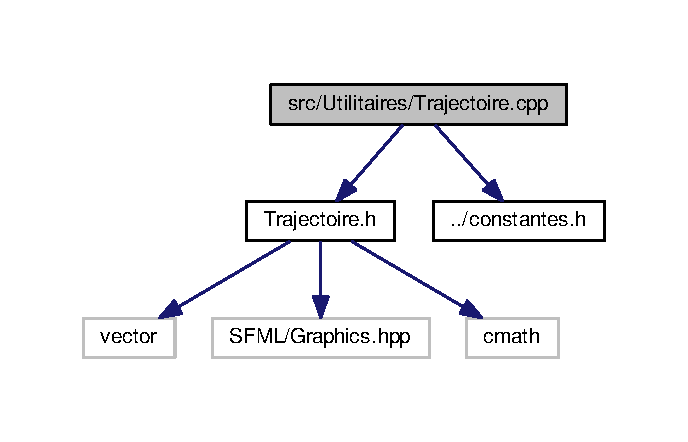
\includegraphics[width=330pt]{_trajectoire_8cpp__incl}
\end{center}
\end{figure}
\subsection*{Fonctions}
\begin{DoxyCompactItemize}
\item 
sf\+::\+Vector2f \hyperlink{_trajectoire_8cpp_acb6b19dacbcb60977ea16b36c5888404}{traj\+\_\+position} (\hyperlink{_trajectoire_8h_afa7f6e8323d7ee755d93cd1f6019dd95}{Trajectoire} trajectoire, float t, float vit\+\_\+, sf\+::\+Vector2f pos\+Init, std\+::vector$<$ float $>$ params)
\end{DoxyCompactItemize}


\subsection{Documentation des fonctions}
\mbox{\Hypertarget{_trajectoire_8cpp_acb6b19dacbcb60977ea16b36c5888404}\label{_trajectoire_8cpp_acb6b19dacbcb60977ea16b36c5888404}} 
\index{Trajectoire.\+cpp@{Trajectoire.\+cpp}!traj\+\_\+position@{traj\+\_\+position}}
\index{traj\+\_\+position@{traj\+\_\+position}!Trajectoire.\+cpp@{Trajectoire.\+cpp}}
\subsubsection{\texorpdfstring{traj\+\_\+position()}{traj\_position()}}
{\footnotesize\ttfamily sf\+::\+Vector2f traj\+\_\+position (\begin{DoxyParamCaption}\item[{\hyperlink{_trajectoire_8h_afa7f6e8323d7ee755d93cd1f6019dd95}{Trajectoire}}]{trajectoire,  }\item[{float}]{t,  }\item[{float}]{vit\+\_\+,  }\item[{sf\+::\+Vector2f}]{pos\+Init,  }\item[{std\+::vector$<$ float $>$}]{params }\end{DoxyParamCaption})}


\hypertarget{_trajectoire_8h}{}\section{Référence du fichier src/\+Utilitaires/\+Trajectoire.h}
\label{_trajectoire_8h}\index{src/\+Utilitaires/\+Trajectoire.\+h@{src/\+Utilitaires/\+Trajectoire.\+h}}
{\ttfamily \#include $<$vector$>$}\newline
{\ttfamily \#include $<$S\+F\+M\+L/\+Graphics.\+hpp$>$}\newline
{\ttfamily \#include $<$cmath$>$}\newline
Graphe des dépendances par inclusion de Trajectoire.\+h\+:\nopagebreak
\begin{figure}[H]
\begin{center}
\leavevmode
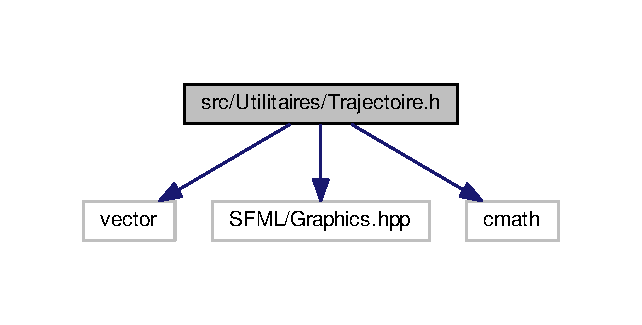
\includegraphics[width=308pt]{_trajectoire_8h__incl}
\end{center}
\end{figure}
Ce graphe montre quels fichiers incluent directement ou indirectement ce fichier \+:\nopagebreak
\begin{figure}[H]
\begin{center}
\leavevmode
\includegraphics[width=350pt]{_trajectoire_8h__dep__incl}
\end{center}
\end{figure}
\subsection*{Énumérations}
\begin{DoxyCompactItemize}
\item 
enum \hyperlink{_trajectoire_8h_afa7f6e8323d7ee755d93cd1f6019dd95}{Trajectoire} \{ \hyperlink{_trajectoire_8h_afa7f6e8323d7ee755d93cd1f6019dd95a8bc010f4818a3f1553fbb13140ef7764}{L\+I\+N\+E\+A\+I\+RE}, 
\hyperlink{_trajectoire_8h_afa7f6e8323d7ee755d93cd1f6019dd95a2e1c07250c4de3cf6c0db9a42dd0870b}{P\+A\+R\+A\+B\+O\+L\+I\+Q\+UE}, 
\hyperlink{_trajectoire_8h_afa7f6e8323d7ee755d93cd1f6019dd95a33f374dc94a3ff34a023886c4e6e7102}{S\+I\+N\+US}, 
\hyperlink{_trajectoire_8h_afa7f6e8323d7ee755d93cd1f6019dd95a90e1b7efef28fa0dc94c0af827f8c5a9}{M\+O\+U\+T\+ON}
 \}\begin{DoxyCompactList}\small\item\em liste �num�r�e des types possibles de trajectoire \end{DoxyCompactList}
\end{DoxyCompactItemize}
\subsection*{Fonctions}
\begin{DoxyCompactItemize}
\item 
sf\+::\+Vector2f \hyperlink{_trajectoire_8h_acb6b19dacbcb60977ea16b36c5888404}{traj\+\_\+position} (\hyperlink{_trajectoire_8h_afa7f6e8323d7ee755d93cd1f6019dd95}{Trajectoire} trajectoire, float t, float vit\+\_\+, sf\+::\+Vector2f pos\+Init, std\+::vector$<$ float $>$ params)
\end{DoxyCompactItemize}


\subsection{Documentation du type de l\textquotesingle{}énumération}
\mbox{\Hypertarget{_trajectoire_8h_afa7f6e8323d7ee755d93cd1f6019dd95}\label{_trajectoire_8h_afa7f6e8323d7ee755d93cd1f6019dd95}} 
\index{Trajectoire.\+h@{Trajectoire.\+h}!Trajectoire@{Trajectoire}}
\index{Trajectoire@{Trajectoire}!Trajectoire.\+h@{Trajectoire.\+h}}
\subsubsection{\texorpdfstring{Trajectoire}{Trajectoire}}
{\footnotesize\ttfamily enum \hyperlink{_trajectoire_8h_afa7f6e8323d7ee755d93cd1f6019dd95}{Trajectoire}}



liste �num�r�e des types possibles de trajectoire 

\begin{DoxyEnumFields}{Valeurs énumérées}
\raisebox{\heightof{T}}[0pt][0pt]{\index{L\+I\+N\+E\+A\+I\+RE@{L\+I\+N\+E\+A\+I\+RE}!Trajectoire.\+h@{Trajectoire.\+h}}\index{Trajectoire.\+h@{Trajectoire.\+h}!L\+I\+N\+E\+A\+I\+RE@{L\+I\+N\+E\+A\+I\+RE}}}\mbox{\Hypertarget{_trajectoire_8h_afa7f6e8323d7ee755d93cd1f6019dd95a8bc010f4818a3f1553fbb13140ef7764}\label{_trajectoire_8h_afa7f6e8323d7ee755d93cd1f6019dd95a8bc010f4818a3f1553fbb13140ef7764}} 
L\+I\+N\+E\+A\+I\+RE&\\
\hline

\raisebox{\heightof{T}}[0pt][0pt]{\index{P\+A\+R\+A\+B\+O\+L\+I\+Q\+UE@{P\+A\+R\+A\+B\+O\+L\+I\+Q\+UE}!Trajectoire.\+h@{Trajectoire.\+h}}\index{Trajectoire.\+h@{Trajectoire.\+h}!P\+A\+R\+A\+B\+O\+L\+I\+Q\+UE@{P\+A\+R\+A\+B\+O\+L\+I\+Q\+UE}}}\mbox{\Hypertarget{_trajectoire_8h_afa7f6e8323d7ee755d93cd1f6019dd95a2e1c07250c4de3cf6c0db9a42dd0870b}\label{_trajectoire_8h_afa7f6e8323d7ee755d93cd1f6019dd95a2e1c07250c4de3cf6c0db9a42dd0870b}} 
P\+A\+R\+A\+B\+O\+L\+I\+Q\+UE&\\
\hline

\raisebox{\heightof{T}}[0pt][0pt]{\index{S\+I\+N\+US@{S\+I\+N\+US}!Trajectoire.\+h@{Trajectoire.\+h}}\index{Trajectoire.\+h@{Trajectoire.\+h}!S\+I\+N\+US@{S\+I\+N\+US}}}\mbox{\Hypertarget{_trajectoire_8h_afa7f6e8323d7ee755d93cd1f6019dd95a33f374dc94a3ff34a023886c4e6e7102}\label{_trajectoire_8h_afa7f6e8323d7ee755d93cd1f6019dd95a33f374dc94a3ff34a023886c4e6e7102}} 
S\+I\+N\+US&\\
\hline

\raisebox{\heightof{T}}[0pt][0pt]{\index{M\+O\+U\+T\+ON@{M\+O\+U\+T\+ON}!Trajectoire.\+h@{Trajectoire.\+h}}\index{Trajectoire.\+h@{Trajectoire.\+h}!M\+O\+U\+T\+ON@{M\+O\+U\+T\+ON}}}\mbox{\Hypertarget{_trajectoire_8h_afa7f6e8323d7ee755d93cd1f6019dd95a90e1b7efef28fa0dc94c0af827f8c5a9}\label{_trajectoire_8h_afa7f6e8323d7ee755d93cd1f6019dd95a90e1b7efef28fa0dc94c0af827f8c5a9}} 
M\+O\+U\+T\+ON&\\
\hline

\end{DoxyEnumFields}


\subsection{Documentation des fonctions}
\mbox{\Hypertarget{_trajectoire_8h_acb6b19dacbcb60977ea16b36c5888404}\label{_trajectoire_8h_acb6b19dacbcb60977ea16b36c5888404}} 
\index{Trajectoire.\+h@{Trajectoire.\+h}!traj\+\_\+position@{traj\+\_\+position}}
\index{traj\+\_\+position@{traj\+\_\+position}!Trajectoire.\+h@{Trajectoire.\+h}}
\subsubsection{\texorpdfstring{traj\+\_\+position()}{traj\_position()}}
{\footnotesize\ttfamily sf\+::\+Vector2f traj\+\_\+position (\begin{DoxyParamCaption}\item[{\hyperlink{_trajectoire_8h_afa7f6e8323d7ee755d93cd1f6019dd95}{Trajectoire}}]{trajectoire,  }\item[{float}]{t,  }\item[{float}]{vit\+\_\+,  }\item[{sf\+::\+Vector2f}]{pos\+Init,  }\item[{std\+::vector$<$ float $>$}]{params }\end{DoxyParamCaption})}


\hypertarget{__vaisseaux_8h}{}\section{src/\+Vaisseau/\+\_\+vaisseaux.h File Reference}
\label{__vaisseaux_8h}\index{src/\+Vaisseau/\+\_\+vaisseaux.\+h@{src/\+Vaisseau/\+\_\+vaisseaux.\+h}}
{\ttfamily \#include \char`\"{}Vaisseau\+Eclaireur.\+h\char`\"{}}\newline
{\ttfamily \#include \char`\"{}Vaisseau\+Test.\+h\char`\"{}}\newline
{\ttfamily \#include \char`\"{}Vaisseau\+Attaquant.\+h\char`\"{}}\newline
{\ttfamily \#include \char`\"{}Vaisseau\+Defenseur.\+h\char`\"{}}\newline

\hypertarget{_vaisseau_8cpp}{}\section{Référence du fichier src/\+Vaisseau/\+Vaisseau.cpp}
\label{_vaisseau_8cpp}\index{src/\+Vaisseau/\+Vaisseau.\+cpp@{src/\+Vaisseau/\+Vaisseau.\+cpp}}
{\ttfamily \#include $<$vector$>$}\newline
{\ttfamily \#include $<$string$>$}\newline
{\ttfamily \#include $<$algorithm$>$}\newline
{\ttfamily \#include \char`\"{}../\+Capacites/\+Capacite.\+h\char`\"{}}\newline
{\ttfamily \#include \char`\"{}Vaisseau.\+h\char`\"{}}\newline
{\ttfamily \#include \char`\"{}../\+Projectiles/\+Projectile.\+h\char`\"{}}\newline
Graphe des dépendances par inclusion de Vaisseau.\+cpp\+:
\nopagebreak
\begin{figure}[H]
\begin{center}
\leavevmode
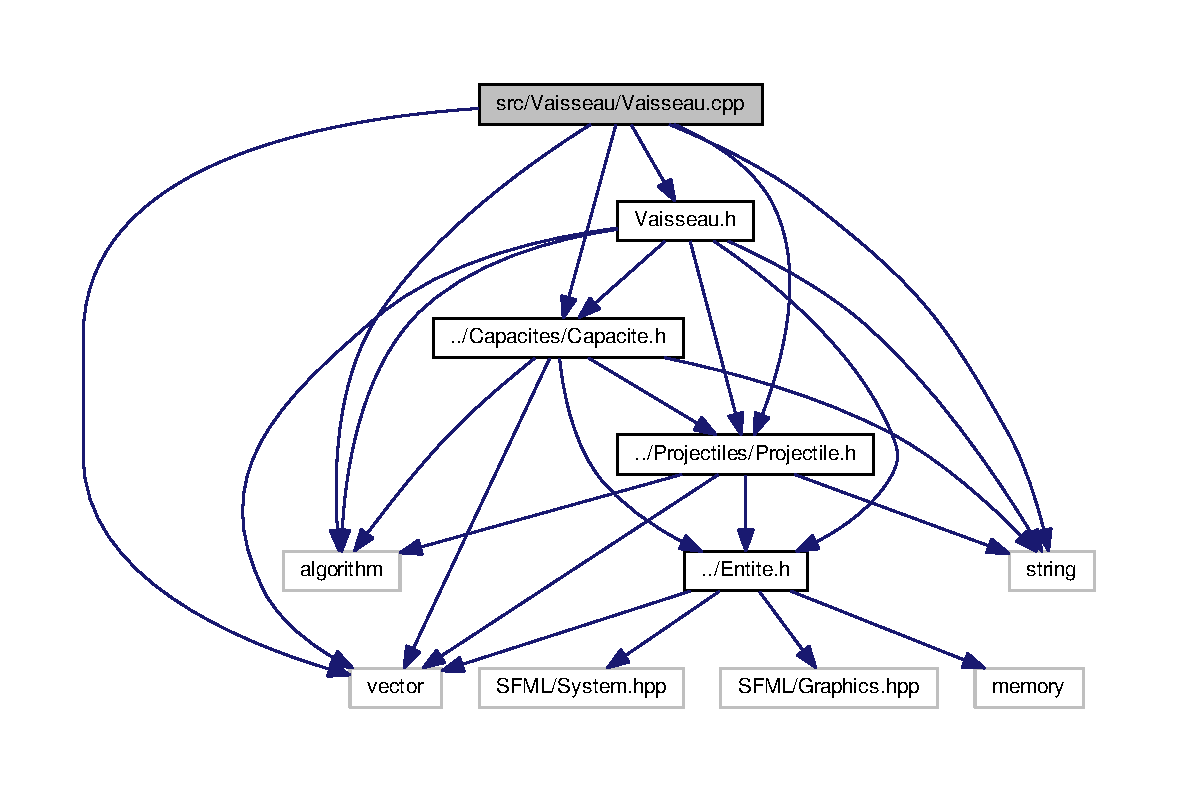
\includegraphics[width=350pt]{_vaisseau_8cpp__incl}
\end{center}
\end{figure}

\hypertarget{_vaisseau_8h}{}\section{Référence du fichier src/\+Vaisseau/\+Vaisseau.h}
\label{_vaisseau_8h}\index{src/\+Vaisseau/\+Vaisseau.\+h@{src/\+Vaisseau/\+Vaisseau.\+h}}
{\ttfamily \#include $<$vector$>$}\newline
{\ttfamily \#include $<$string$>$}\newline
{\ttfamily \#include $<$algorithm$>$}\newline
{\ttfamily \#include \char`\"{}../\+Capacites/\+Capacite.\+h\char`\"{}}\newline
{\ttfamily \#include \char`\"{}../\+Entite.\+h\char`\"{}}\newline
{\ttfamily \#include \char`\"{}../\+Projectiles/\+Projectile.\+h\char`\"{}}\newline
Graphe des dépendances par inclusion de Vaisseau.\+h\+:\nopagebreak
\begin{figure}[H]
\begin{center}
\leavevmode
\includegraphics[width=350pt]{_vaisseau_8h__incl}
\end{center}
\end{figure}
Ce graphe montre quels fichiers incluent directement ou indirectement ce fichier \+:\nopagebreak
\begin{figure}[H]
\begin{center}
\leavevmode
\includegraphics[width=350pt]{_vaisseau_8h__dep__incl}
\end{center}
\end{figure}
\subsection*{Classes}
\begin{DoxyCompactItemize}
\item 
class \hyperlink{class_vaisseau}{Vaisseau}
\begin{DoxyCompactList}\small\item\em classe du vaisseau (véhicule) d\textquotesingle{}un joueur ou d\textquotesingle{}un ennemi \end{DoxyCompactList}\end{DoxyCompactItemize}

\hypertarget{_vaisseau_attaquant_8cpp}{}\section{Référence du fichier src/\+Vaisseau/\+Vaisseau\+Attaquant.cpp}
\label{_vaisseau_attaquant_8cpp}\index{src/\+Vaisseau/\+Vaisseau\+Attaquant.\+cpp@{src/\+Vaisseau/\+Vaisseau\+Attaquant.\+cpp}}
{\ttfamily \#include \char`\"{}Vaisseau\+Attaquant.\+h\char`\"{}}\newline
{\ttfamily \#include $<$cmath$>$}\newline
Graphe des dépendances par inclusion de Vaisseau\+Attaquant.\+cpp\+:\nopagebreak
\begin{figure}[H]
\begin{center}
\leavevmode
\includegraphics[width=350pt]{_vaisseau_attaquant_8cpp__incl}
\end{center}
\end{figure}

\hypertarget{_vaisseau_attaquant_8h}{}\section{src/\+Vaisseau/\+Vaisseau\+Attaquant.h File Reference}
\label{_vaisseau_attaquant_8h}\index{src/\+Vaisseau/\+Vaisseau\+Attaquant.\+h@{src/\+Vaisseau/\+Vaisseau\+Attaquant.\+h}}
{\ttfamily \#include \char`\"{}../constantes.\+h\char`\"{}}\newline
{\ttfamily \#include \char`\"{}Vaisseau.\+h\char`\"{}}\newline
{\ttfamily \#include \char`\"{}../\+Capacites/\+Cap\+Missile.\+h\char`\"{}}\newline
{\ttfamily \#include \char`\"{}../\+Utilitaires/\+Trajectoire.\+h\char`\"{}}\newline
\subsection*{Classes}
\begin{DoxyCompactItemize}
\item 
class \mbox{\hyperlink{class_vaisseau_attaquant}{Vaisseau\+Attaquant}}
\begin{DoxyCompactList}\small\item\em classe d\textquotesingle{}un ennemi de base \+: l\textquotesingle{}attaquant \end{DoxyCompactList}\end{DoxyCompactItemize}

\hypertarget{_vaisseau_defenseur_8cpp}{}\section{src/\+Vaisseau/\+Vaisseau\+Defenseur.cpp File Reference}
\label{_vaisseau_defenseur_8cpp}\index{src/\+Vaisseau/\+Vaisseau\+Defenseur.\+cpp@{src/\+Vaisseau/\+Vaisseau\+Defenseur.\+cpp}}
{\ttfamily \#include \char`\"{}Vaisseau\+Defenseur.\+h\char`\"{}}\newline
{\ttfamily \#include $<$cmath$>$}\newline

\hypertarget{_vaisseau_defenseur_8h}{}\section{Référence du fichier src/\+Vaisseau/\+Vaisseau\+Defenseur.h}
\label{_vaisseau_defenseur_8h}\index{src/\+Vaisseau/\+Vaisseau\+Defenseur.\+h@{src/\+Vaisseau/\+Vaisseau\+Defenseur.\+h}}
{\ttfamily \#include $<$vector$>$}\newline
{\ttfamily \#include \char`\"{}../constantes.\+h\char`\"{}}\newline
{\ttfamily \#include \char`\"{}Vaisseau.\+h\char`\"{}}\newline
{\ttfamily \#include \char`\"{}../\+Utilitaires/\+Trajectoire.\+h\char`\"{}}\newline
{\ttfamily \#include \char`\"{}Vaisseau\+Defenseur\+B.\+h\char`\"{}}\newline
Graphe des dépendances par inclusion de Vaisseau\+Defenseur.\+h\+:\nopagebreak
\begin{figure}[H]
\begin{center}
\leavevmode
\includegraphics[width=350pt]{_vaisseau_defenseur_8h__incl}
\end{center}
\end{figure}
Ce graphe montre quels fichiers incluent directement ou indirectement ce fichier \+:\nopagebreak
\begin{figure}[H]
\begin{center}
\leavevmode
\includegraphics[width=350pt]{_vaisseau_defenseur_8h__dep__incl}
\end{center}
\end{figure}
\subsection*{Classes}
\begin{DoxyCompactItemize}
\item 
class \hyperlink{class_vaisseau_defenseur}{Vaisseau\+Defenseur}
\end{DoxyCompactItemize}

\hypertarget{_vaisseau_defenseur_b_8cpp}{}\section{Référence du fichier src/\+Vaisseau/\+Vaisseau\+DefenseurB.cpp}
\label{_vaisseau_defenseur_b_8cpp}\index{src/\+Vaisseau/\+Vaisseau\+Defenseur\+B.\+cpp@{src/\+Vaisseau/\+Vaisseau\+Defenseur\+B.\+cpp}}
{\ttfamily \#include \char`\"{}Vaisseau\+Defenseur\+B.\+h\char`\"{}}\newline
{\ttfamily \#include $<$cmath$>$}\newline
Graphe des dépendances par inclusion de Vaisseau\+Defenseur\+B.\+cpp\+:\nopagebreak
\begin{figure}[H]
\begin{center}
\leavevmode
\includegraphics[width=350pt]{_vaisseau_defenseur_b_8cpp__incl}
\end{center}
\end{figure}

\hypertarget{_vaisseau_defenseur_b_8h}{}\section{Référence du fichier src/\+Vaisseau/\+Vaisseau\+DefenseurB.h}
\label{_vaisseau_defenseur_b_8h}\index{src/\+Vaisseau/\+Vaisseau\+Defenseur\+B.\+h@{src/\+Vaisseau/\+Vaisseau\+Defenseur\+B.\+h}}
{\ttfamily \#include \char`\"{}Vaisseau.\+h\char`\"{}}\newline
Graphe des dépendances par inclusion de Vaisseau\+Defenseur\+B.\+h\+:\nopagebreak
\begin{figure}[H]
\begin{center}
\leavevmode
\includegraphics[width=350pt]{_vaisseau_defenseur_b_8h__incl}
\end{center}
\end{figure}
Ce graphe montre quels fichiers incluent directement ou indirectement ce fichier \+:\nopagebreak
\begin{figure}[H]
\begin{center}
\leavevmode
\includegraphics[width=350pt]{_vaisseau_defenseur_b_8h__dep__incl}
\end{center}
\end{figure}
\subsection*{Classes}
\begin{DoxyCompactItemize}
\item 
class \hyperlink{class_vaisseau_defenseur_b}{Vaisseau\+DefenseurB}
\begin{DoxyCompactList}\small\item\em classe du bouclier du \hyperlink{class_vaisseau_defenseur}{Vaisseau\+Defenseur} \end{DoxyCompactList}\end{DoxyCompactItemize}

\hypertarget{_vaisseau_eclaireur_8cpp}{}\section{src/\+Vaisseau/\+Vaisseau\+Eclaireur.cpp File Reference}
\label{_vaisseau_eclaireur_8cpp}\index{src/\+Vaisseau/\+Vaisseau\+Eclaireur.\+cpp@{src/\+Vaisseau/\+Vaisseau\+Eclaireur.\+cpp}}
{\ttfamily \#include \char`\"{}Vaisseau\+Eclaireur.\+h\char`\"{}}\newline
{\ttfamily \#include $<$cmath$>$}\newline
{\ttfamily \#include $<$iostream$>$}\newline

\hypertarget{_vaisseau_eclaireur_8h}{}\section{Référence du fichier src/\+Vaisseau/\+Vaisseau\+Eclaireur.h}
\label{_vaisseau_eclaireur_8h}\index{src/\+Vaisseau/\+Vaisseau\+Eclaireur.\+h@{src/\+Vaisseau/\+Vaisseau\+Eclaireur.\+h}}
{\ttfamily \#include $<$vector$>$}\newline
{\ttfamily \#include \char`\"{}../constantes.\+h\char`\"{}}\newline
{\ttfamily \#include \char`\"{}Vaisseau.\+h\char`\"{}}\newline
{\ttfamily \#include \char`\"{}../\+Utilitaires/\+Trajectoire.\+h\char`\"{}}\newline
Graphe des dépendances par inclusion de Vaisseau\+Eclaireur.\+h\+:\nopagebreak
\begin{figure}[H]
\begin{center}
\leavevmode
\includegraphics[width=350pt]{_vaisseau_eclaireur_8h__incl}
\end{center}
\end{figure}
Ce graphe montre quels fichiers incluent directement ou indirectement ce fichier \+:\nopagebreak
\begin{figure}[H]
\begin{center}
\leavevmode
\includegraphics[width=350pt]{_vaisseau_eclaireur_8h__dep__incl}
\end{center}
\end{figure}
\subsection*{Classes}
\begin{DoxyCompactItemize}
\item 
class \hyperlink{class_vaisseau_eclaireur}{Vaisseau\+Eclaireur}
\begin{DoxyCompactList}\small\item\em classe d\textquotesingle{}un ennemi de base \+: l\textquotesingle{}éclaireur \end{DoxyCompactList}\end{DoxyCompactItemize}

\hypertarget{_vaisseau_test_8cpp}{}\section{Référence du fichier src/\+Vaisseau/\+Vaisseau\+Test.cpp}
\label{_vaisseau_test_8cpp}\index{src/\+Vaisseau/\+Vaisseau\+Test.\+cpp@{src/\+Vaisseau/\+Vaisseau\+Test.\+cpp}}
{\ttfamily \#include \char`\"{}Vaisseau\+Test.\+h\char`\"{}}\newline
{\ttfamily \#include $<$cmath$>$}\newline
Graphe des dépendances par inclusion de Vaisseau\+Test.\+cpp\+:\nopagebreak
\begin{figure}[H]
\begin{center}
\leavevmode
\includegraphics[width=350pt]{_vaisseau_test_8cpp__incl}
\end{center}
\end{figure}

\hypertarget{_vaisseau_test_8h}{}\section{Référence du fichier src/\+Vaisseau/\+Vaisseau\+Test.h}
\label{_vaisseau_test_8h}\index{src/\+Vaisseau/\+Vaisseau\+Test.\+h@{src/\+Vaisseau/\+Vaisseau\+Test.\+h}}
{\ttfamily \#include \char`\"{}Vaisseau.\+h\char`\"{}}\newline
{\ttfamily \#include \char`\"{}../\+Capacites/\+Capacite.\+h\char`\"{}}\newline
{\ttfamily \#include \char`\"{}../\+Capacites/\+\_\+\+Capacites.\+h\char`\"{}}\newline
Graphe des dépendances par inclusion de Vaisseau\+Test.\+h\+:
% FIG 0
Ce graphe montre quels fichiers incluent directement ou indirectement ce fichier \+:
% FIG 1
\subsection*{Classes}
\begin{DoxyCompactItemize}
\item 
class \hyperlink{class_vaisseau_test}{Vaisseau\+Test}
\end{DoxyCompactItemize}

%--- End generated contents ---

% Index
\backmatter
\newpage
\phantomsection
\clearemptydoublepage
\addcontentsline{toc}{chapter}{Index}
\printindex

\end{document}
